% Options for packages loaded elsewhere
\PassOptionsToPackage{unicode}{hyperref}
\PassOptionsToPackage{hyphens}{url}
%
\documentclass[
]{book}
\usepackage{lmodern}
\usepackage{amssymb,amsmath}
\usepackage{ifxetex,ifluatex}
\ifnum 0\ifxetex 1\fi\ifluatex 1\fi=0 % if pdftex
  \usepackage[T1]{fontenc}
  \usepackage[utf8]{inputenc}
  \usepackage{textcomp} % provide euro and other symbols
\else % if luatex or xetex
  \usepackage{unicode-math}
  \defaultfontfeatures{Scale=MatchLowercase}
  \defaultfontfeatures[\rmfamily]{Ligatures=TeX,Scale=1}
\fi
% Use upquote if available, for straight quotes in verbatim environments
\IfFileExists{upquote.sty}{\usepackage{upquote}}{}
\IfFileExists{microtype.sty}{% use microtype if available
  \usepackage[]{microtype}
  \UseMicrotypeSet[protrusion]{basicmath} % disable protrusion for tt fonts
}{}
\makeatletter
\@ifundefined{KOMAClassName}{% if non-KOMA class
  \IfFileExists{parskip.sty}{%
    \usepackage{parskip}
  }{% else
    \setlength{\parindent}{0pt}
    \setlength{\parskip}{6pt plus 2pt minus 1pt}}
}{% if KOMA class
  \KOMAoptions{parskip=half}}
\makeatother
\usepackage{xcolor}
\IfFileExists{xurl.sty}{\usepackage{xurl}}{} % add URL line breaks if available
\IfFileExists{bookmark.sty}{\usepackage{bookmark}}{\usepackage{hyperref}}
\hypersetup{
  pdftitle={Mathematical Knowledge for Secondary Teachers},
  pdfauthor={Jim Gleason and Martha Makowski},
  hidelinks,
  pdfcreator={LaTeX via pandoc}}
\urlstyle{same} % disable monospaced font for URLs
\usepackage{longtable,booktabs}
% Correct order of tables after \paragraph or \subparagraph
\usepackage{etoolbox}
\makeatletter
\patchcmd\longtable{\par}{\if@noskipsec\mbox{}\fi\par}{}{}
\makeatother
% Allow footnotes in longtable head/foot
\IfFileExists{footnotehyper.sty}{\usepackage{footnotehyper}}{\usepackage{footnote}}
\makesavenoteenv{longtable}
\usepackage{graphicx,grffile}
\makeatletter
\def\maxwidth{\ifdim\Gin@nat@width>\linewidth\linewidth\else\Gin@nat@width\fi}
\def\maxheight{\ifdim\Gin@nat@height>\textheight\textheight\else\Gin@nat@height\fi}
\makeatother
% Scale images if necessary, so that they will not overflow the page
% margins by default, and it is still possible to overwrite the defaults
% using explicit options in \includegraphics[width, height, ...]{}
\setkeys{Gin}{width=\maxwidth,height=\maxheight,keepaspectratio}
% Set default figure placement to htbp
\makeatletter
\def\fps@figure{htbp}
\makeatother
\setlength{\emergencystretch}{3em} % prevent overfull lines
\providecommand{\tightlist}{%
  \setlength{\itemsep}{0pt}\setlength{\parskip}{0pt}}
\setcounter{secnumdepth}{5}


\usepackage{hieroglf}

%\newtheorem{standards}{Common Core State Standards}

\usepackage[margin=1in]{geometry}
\usepackage{natbib}
\usepackage[]{natbib}
\bibliographystyle{plainnat}

\title{Mathematical Knowledge for Secondary Teachers}
\author{Jim Gleason and Martha Makowski}
\date{}

\usepackage{amsthm}
\newtheorem{theorem}{Theorem}[chapter]
\newtheorem{lemma}{Lemma}[chapter]
\newtheorem{corollary}{Corollary}[chapter]
\newtheorem{proposition}{Proposition}[chapter]
\newtheorem{conjecture}{Conjecture}[chapter]
\theoremstyle{definition}
\newtheorem{definition}{Definition}[chapter]
\theoremstyle{definition}
\newtheorem{example}{Example}[chapter]
\theoremstyle{definition}
\newtheorem{exercise}{Exercise}[chapter]
\theoremstyle{remark}
\newtheorem*{remark}{Remark}
\newtheorem*{solution}{Solution}
\begin{document}
\maketitle

{
\setcounter{tocdepth}{1}
\tableofcontents
}
\hypertarget{section}{%
\chapter*{}\label{section}}
\addcontentsline{toc}{chapter}{}

\begin{center}
\includegraphics[width=0.5\linewidth]{images/Cover} \end{center}

© 2021 Jim Gleason and Martha Makowski

\hypertarget{preface}{%
\chapter*{Preface}\label{preface}}
\addcontentsline{toc}{chapter}{Preface}

The knowledge possessed by an excellent secondary mathematics teacher draws on a variety of skills, beliefs, and passions related to the practice of teaching. A large portion of this knowledge is acquired through experience working with students. However, excellent teachers develop certain aspects of knowledge through structured learning environments like a textbook or university course.

This textbook is inspired by \citet{Usiskin2003} and designed to help current and future teachers explore a unique blend of \emph{mathematical content knowledge} used in the practice of teaching mathematics at the secondary and early post-secondary level. Content examining how K-12 students learn mathematics or on classroom management techniques related to mathematical teaching are left to other texts. There are many excellent resources for this pedagogical content knowledge, particularly from the National Council of Teachers of Mathematics (NCTM) and the Association of Mathematics Teacher Educators (AMTE).

\hypertarget{for-the-student}{%
\section*{For the Student}\label{for-the-student}}
\addcontentsline{toc}{section}{For the Student}

\hypertarget{for-the-instructor}{%
\section*{For the Instructor}\label{for-the-instructor}}
\addcontentsline{toc}{section}{For the Instructor}

\hypertarget{one-semester-course}{%
\subsection*{One Semester Course}\label{one-semester-course}}
\addcontentsline{toc}{subsection}{One Semester Course}

\hypertarget{two-semester-courses}{%
\subsection*{Two Semester Courses}\label{two-semester-courses}}
\addcontentsline{toc}{subsection}{Two Semester Courses}

\hypertarget{three-semester-courses}{%
\subsection*{Three Semester Courses}\label{three-semester-courses}}
\addcontentsline{toc}{subsection}{Three Semester Courses}

\hypertarget{focus-on-middle-school-content}{%
\subsection*{Focus on Middle School Content}\label{focus-on-middle-school-content}}
\addcontentsline{toc}{subsection}{Focus on Middle School Content}

\hypertarget{acknowledgements}{%
\chapter*{Acknowledgements}\label{acknowledgements}}
\addcontentsline{toc}{chapter}{Acknowledgements}

\hypertarget{part-foundations}{%
\part{FOUNDATIONS}\label{part-foundations}}

\hypertarget{ch:MathEdFoundations}{%
\chapter{Mathematics Education Foundations}\label{ch:MathEdFoundations}}

This first chapter focuses on developing the notion of Mathematical Knowledge for Teaching and examining how content knowledge supports the current standards for mathematical practice and the content standards developed by various educational researchers and mathematics education organizations. Understanding these foundations prior to jumping into the rest of the content provides both an organizational framework and a foundation for the topics covered. Some of these ideas may challenge your ways of thinking, while others reinforce what you already know. We encourage you to go beyond what is written here and to read some of the original research articles and organization standards cited in this chapter.

\begin{figure}

{\centering 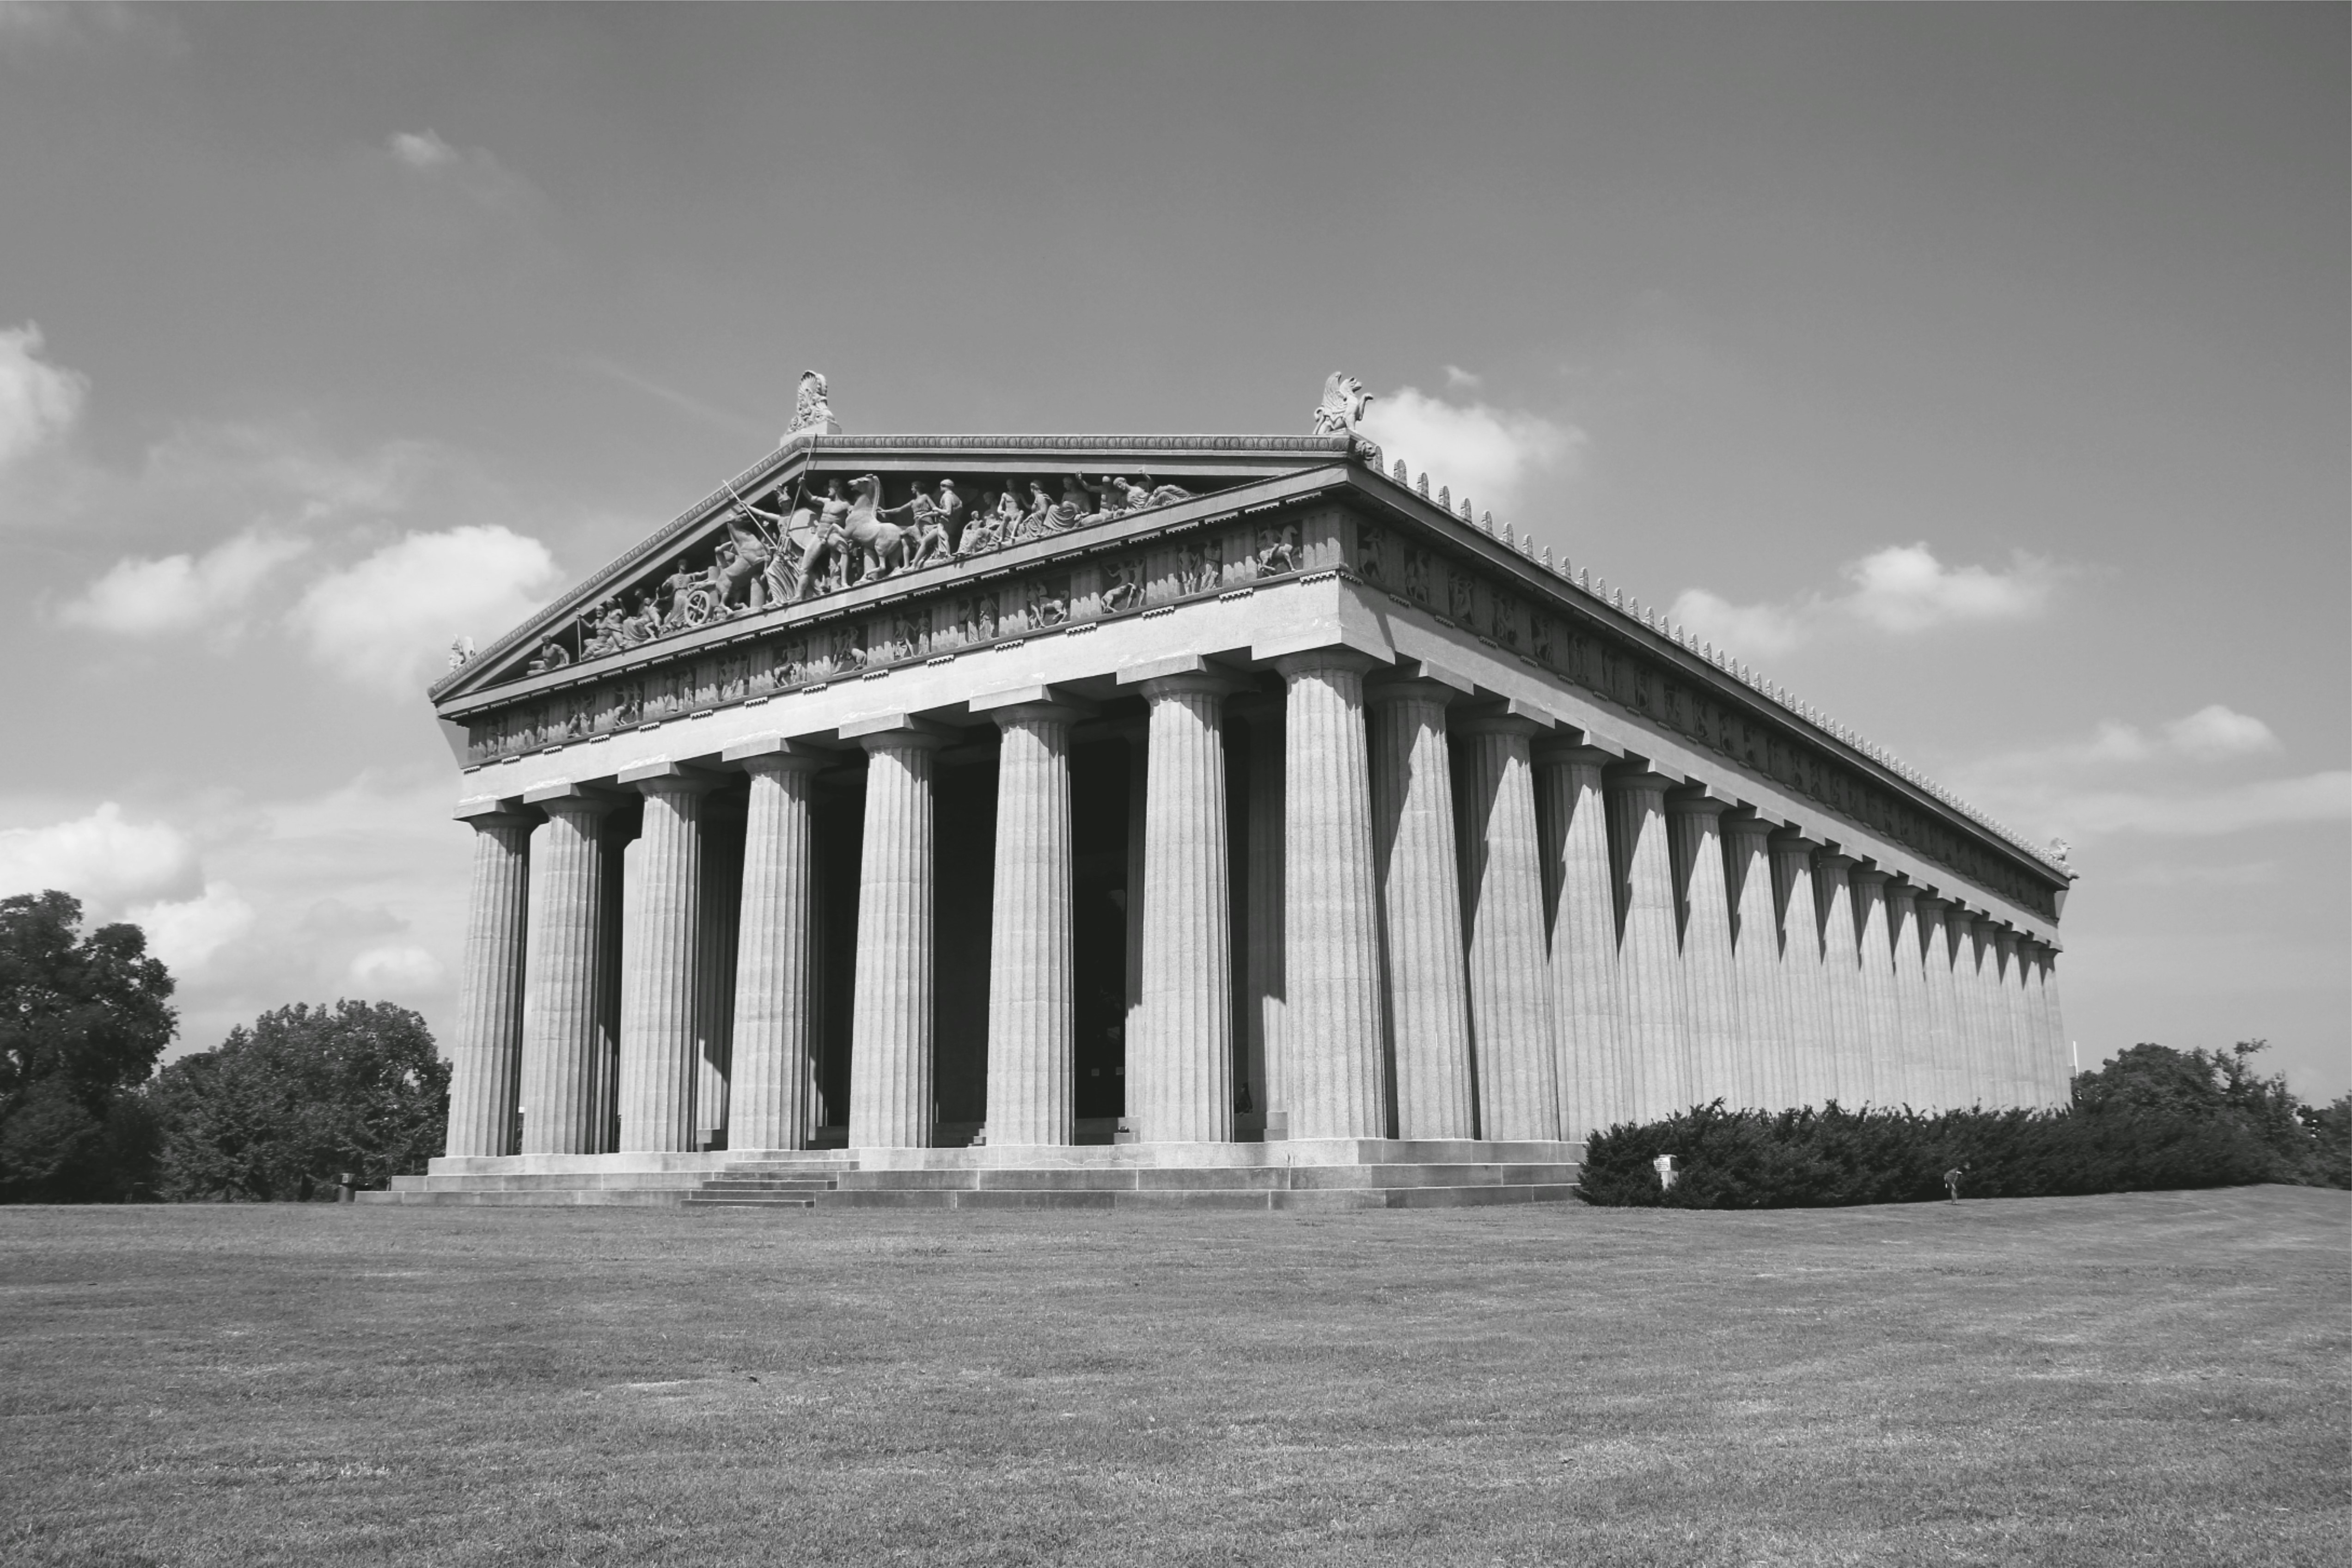
\includegraphics[width=0.7\linewidth]{images/Parthenon_Nashville_bw} 

}

\end{figure}

\newpage

\hypertarget{section:MKT}{%
\section{Mathematical Knowledge for Teaching}\label{section:MKT}}

In his presidential address to the American Educational Research Association, Lee Shulman (\citet{shulman1986}) popularized the concept of knowledge for teaching that included a specialized content knowledge where ``the teacher need not only understand \emph{that} something is so; the teacher must further understand \emph{why} it is so, on what grounds its warrant can be asserted, and under what circumstances our belief in its justification'' (p.~9). Researchers in mathematics education further expanded on this idea in the development of domains of Mathematical Knowledge for Teaching. This textbook focuses on the Subject Matter Knowledge side of the Mathematical Knowledge for Teaching.

\begin{figure}

{\centering 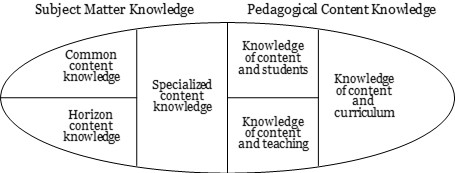
\includegraphics[width=1\linewidth]{tikz/ballegg1} 

}

\caption{Domains of Mathematical Knowledge for Teaching [@Ball2008]}\label{fig:unnamed-chunk-3}
\end{figure}

\hypertarget{common-content-knowledge}{%
\subsection{Common Content Knowledge}\label{common-content-knowledge}}

The foundation for much of the other aspects of mathematical knowledge for teaching is \textbf{common content knowledge}, defined as ``the mathematical knowledge and skill used in settings other than teaching'' \citep[p.~399]{Ball2008}. Common content knowledge provides the individual the ability to solve mathematical problems from the related curriculum and to apply the mathematical knowledge to other fields of knowledge outside of mathematics. Common content knowledge also includes understanding how some of the different mathematical subjects build upon one another, but does not require those studying the material to be able to explain broader patterns. Thus, common content knowledge represents the type of knowledge that we expect secondary and introductory post-secondary students to display.

For instance, common content knowledge related to rational algebraic expressions and functions includes understanding the relationships between rational expressions and rational numbers, how long-division of polynomials relates to long-division of integers, and the properties of the quotient and remainder of a rational expression and its effect on the graph of the related function. While this common content knowledge includes a deeper level of knowledge and a richer web of conceptual understanding by the teacher than is common for most K-12 students, the knowledge still falls within the expectations for the most advanced of these K-12 students. Thus, it is paramount that secondary mathematics teachers develop deep fluency in common content knowledge and the interconnectedness of the many different mathematical concepts in the curriculum. Such a deep and interconnected knowledge base of the teacher provides a requisite foundation in helping K-12 students learn mathematics. However, it is only a first step.

\hypertarget{specialized-content-knowledge}{%
\subsection{Specialized Content Knowledge}\label{specialized-content-knowledge}}

\textbf{Specialized content knowledge} incorporates mathematical knowledge that goes beyond knowledge expected of students, with a focus on the mathematical knowledge that improves the ability of the teacher to assist students learning mathematics \citep[p.~400]{Ball2008}. Thus, specialized content knowledge supplements the common content knowledge that all K-12 students of mathematics need. For example, while common content knowledge for rational algebraic expressions and rational functions include the relationships to the rational numbers, specialized content knowledge could include knowledge of rings and integral domains, thereby improving the teacher's ability to help students to make the connections between various pieces of related content knowledge.

A teacher would also use this specialized content knowledge related to rational expressions when explaining the extent to which two rational expressions are equivalent when common factors of the numerator and denominator cancel. For instance the teacher could explain the ways in which the expressions
\[ \frac{(x-1)(x+2)^2}{(x+1)(x+2)} \quad \mbox{and} \quad \frac{(x-1)(x+2)}{(x+1)}\] are equivalent and distinct.

\hypertarget{horizon-content-knowledge}{%
\subsection{Horizon Content Knowledge}\label{horizon-content-knowledge}}

Excellent teachers use more than just a knowledge of the content in the current curriculum when teaching students. They also draw on knowledge of what their students have previously learned in mathematics, what mathematics content will be covered in the next few years, and how the current mathematical topic relates to applications outside of mathematics. That is, excellent mathematics teachers see their instruction as part of a continuum, of which their work is only a small part. We call this domain of knowledge \textbf{horizon content knowledge}.

For example, a teacher with horizon content knowledge might use students' familiarity with rational numbers to help high school students develop knowledge of rational algebraic expressions and functions. She could also use her knowledge from differential equations to know that the rational functions play a pivotal role in the Laplace transform, helping to determine the amount of time and detail appropriate for teaching about the quotient and remainder theorem for polynomials and how to rewrite rational expressions using partial fractions. The teacher could also use knowledge of the physics curriculum and Boyle's law to help students make connections between rational expressions and functions and other fields of study. While each of these pieces of knowledge are not essential for mathematics teachers, the more knowledge one has, the better that teacher can help students learn and apply the critical components of the content.

\hypertarget{exercises}{%
\subsection{Exercises}\label{exercises}}

\begin{enumerate}
\def\labelenumi{\arabic{enumi}.}
\item
  Consider the general quadratic expression \(ax^2 + bx+c\), where \(a\), \(b\), and \(c\) are real numbers such that \(a\neq0\).

  \begin{enumerate}
  \def\labelenumii{\alph{enumii}.}
  \item
    Write a list of everything you \textbf{know} about the general quadratic expression.
  \item
    Write a list of everything you can \textbf{do} to the general quadratic expression.
  \item
    How are quadratic expressions different than quadratic equations?
  \item
    How does the factorization of a quadratic expression relate to prime numbers?
  \item
    How much do you know about the ways in which quadratic expressions are used outside of mathematics?
  \item
    Review the mathematics standards for quadratic expressions for your state. How many of the things you have listed for parts (a) and (b) match up with those standards?
  \item
    For each of your answers to a. through e., does the content you have listed or described align most with common content knowledge, specialized content knowledge, or horizon content knowledge?
  \end{enumerate}
\item
  Consider a triangle. A particular high school geometry textbook defines a triangle as ``a polygon with three sides.'' A second textbook defines a triangle as ``the figure formed by connecting three non-co-linear points with straight segments.'' A last textbook defines triangles as ``A three-sided figure.''

  \begin{enumerate}
  \def\labelenumii{\alph{enumii})}
  \item
    Are all three definitions accurate, or do some allow for shapes that might not be triangles as you understand them to be included within the category of triangle?
  \item
    In what ways might each definition be considered sloppy? That is, are there any parts of the definition that might not be well-defined? In what ways might each definition make using triangles in future lessons more difficult?
  \item
    What information do you think each textbook has presented prior to giving its definition for a triangle?
  \item
    How might horizon content knowledge help an instructor preparing a lesson on triangles decide whether a definition is appropriate or not for her students?
  \end{enumerate}
\end{enumerate}

\hypertarget{mathematical-practice-standards}{%
\section{Mathematical Practice Standards}\label{mathematical-practice-standards}}

Just like almost all of the content taught in secondary schools, the development of procedural habits and pieces of information are important parts of a secondary education, the heart of learning lies in developing habits of thinking, perseverance techniques, and developing communication skills to improve the ability to interact with the world around them. For example, the United Nations Educational, Scientific, and Cultural Organization (UNESCO) and the United Nations Office on Drugs and Crime (UNODC) \citeyearpar{UNESCO} described cognitive learning outcomes for secondary education such that a student ``Knows about local, national, and global governance and accountability systems and structures, understands issues affecting interaction and connectedness of communities at local, national and global levels, (and) develops skills for critical inquiry and analysis'' (p.~16). Mathematics, despite it's reputation, aligns well with these goals. Critical thinking, reasoning, and communicating are the most important components of the secondary mathematics curriculum, and are often the most ignored.

The National Council of Teachers of Mathematics \citeyearpar{PSSM} describes these goals in the -Principles and Standards for School Mathematics-, giving them the name `Process Standards.' The National Governors Association Center for Best Practices and the Council of Chief State School Officers \citep{CCSS} expanded upon these to create the `Common Core State Standards Standards for Mathematical Practice.' These practice standards are listed in Table \ref{tab:SMPs} and more details about these standards can be found in their corresponding publications.

\begin{table}

\caption{\label{tab:SMPs}NCTM Process Standards and  Common Core Standards for Mathematical Practice}
\centering
\begin{tabular}[t]{l|l}
\hline
Standards for Mathematical Practice & Process Standards\\
\hline
Make sense of problems and persevere in solving them. & Problem Solving\\
\hline
Reason abstractly and quantitatively. & Reasoning and Proof\\
\hline
Construct viable arguments and critique the reasoning of others. & Communication\\
\hline
Model with mathematics. & Connections\\
\hline
Use appropriate tools strategically. & Representations\\
\hline
Attend to precision & \\
\hline
Look for and make use of structure. & \\
\hline
Look for and express regularity in repeated reasoning. & \\
\hline
\end{tabular}
\end{table}

It is worth noting that these practices are expected of students of mathematics at \emph{all} grade levels. In order to help others develop these practices, we must first develop them in ourselves. Only then will we be in a position to create a learning environment that motivates and enables students to grow in these practices.

To support the users of this text in developing these practices, opportunities to practice them are woven into the text, exercises, and projects. However, as any good teacher knows, the learner needs to be actively engaged in order for an objective to be reached. As you work through the text, pay attention to how the arguments are presented and seek to understand the process behind the mathematical content. When completing the exercises and projects, do not just try to get an answer. Instead, take some time to grapple with the ideas, think of better ways to communicate what you do not understand, and seek to understand the deeper connections involved in the task.

For the purpose of this text we group these practice standards into four categories: mathematical problem solving, modeling with mathematics, communicating mathematically, and understanding mathematical structures. We briefly elaborate on each in the following sections.

\hypertarget{mathematical-problem-solving}{%
\subsection{Mathematical Problem Solving}\label{mathematical-problem-solving}}

Mathematical problem solving is perhaps the most widely cited application of mathematics ``in the real world''. Although generally acknowledge as important, problem solving is a complex process that is difficult to teach. In his book \emph{How to Solve It: A new aspect of mathematical method}, George Pólya described four phases of the problem solving process (See Figure \ref{fig:polya} when approaching mathematical problems \citep{Polya1945}. While many others have expanded on this problem solving process, much of the thinking around problem solving still traces back to the four phases that Pólya describes.

\begin{figure}

{\centering 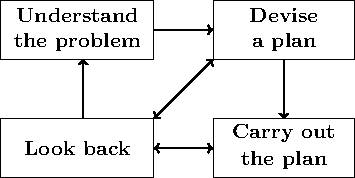
\includegraphics[width=0.45\linewidth]{tikz/polya} 

}

\caption{Pólya's problem solving process}\label{fig:polya}
\end{figure}

The first phase is the process of understanding the problem. What this phase looks like varies by problem, but often involves making sure you understand what information is given and relevant. It also includes knowledge of what an answer should look like for the question posed and, where relevant, being able to organize the provided information in a picture or diagram to better understand the situation. So, for example, if the problem is computational, understanding the problem may entail understanding whether positive or negative answers are valid solutions. If the problem is a theorem that needs proving, this phase may involve generating related examples or writing out relevant definitions to make sure you understand the given inputs and implications of the theorem.

The second phase of the problem solving process is to devise a plan. Many students struggle in the problem solving process because they only want to solve problems for which they have previously been given a template. The origin of this desire has roots in the fact that many teachers only assign students problems that are similar to those discussed in class. True mathematical problem solving involves confronting problems for which the solution is not immediately obvious to the problem solver. In problem solving, one may need to connect the current problem to previously solved problems or restate the problem in a different form with an easier solution process. Sometimes a full plan is not possible at the beginning and the solver needs to just plan initial steps and work through those to gather more information about the problem that will help them create a new plan later in the process.

Once an initial plan is devised, it needs to be carried out. This is often the simplest part of the problem solving process, and often the only component that students complete. With today's technology, computer applications can often complete the details of this part of the problem solving process through statistical analyses, computer algebra systems, or graphical programs.

After the plan is carried out, it is important to look back, completing the final phase of the problem solving process. In this step the problem solver determines whether their solution makes sense in the context of the original problem. For example, in calculus, it is often possible to obtain negative solutions that are not appropriate to the problem posed. The final step of looking back also entails making sure that we have actually addressed the question asked or the problem posed, rather than a different, somewhat related, question or problem.

Although these four phases appear linear, the majority of mathematical problems require various iterations of these phases. In particular, it is often the case that the first plan created to solve a problem does not work, so it has to be revised following an attempt to carry it out. Good problem solvers see these revisions as opportunities to learn more about the problem, rather than as failure at the problem solving process.

\hypertarget{modeling-with-mathematics}{%
\subsection{Modeling with Mathematics}\label{modeling-with-mathematics}}

Mathematical problem solving often relies on modeling with mathematics, particularly in the context of real-world phenomena. The Guidelines for Assessment and Instruction in Mathematical Modeling Education (GAIMME) defines mathematical modeling as ``a process that uses mathematics to represent, analyze, make predictions or otherwise provide insight into real-world phenomena'' \citep[p.~8]{GAIMME}. This definition varies from other common connotations of ``modeling'' that are used in education, including in mathematics. For example in mathematics education, using manipulatives to model a mathematical idea; sketching graphs or pictures to communicate or understand concepts; and demonstrating how to solve certain types of problems are all referred to as modeling. However, as a process standard, modeling mathematics does not generally include these activities. Instead, it refers to activities of using mathematics to analyze, predict, and represent real-world data.

The GAIMME Report breaks the mathematical modeling process into the six components shown in Figure \ref{fig:GAIMME}. Critically, these six components \textbf{do not} happen in a progression, but instead are iterative and sometimes run parallel to each other.

\begin{figure}

{\centering \includegraphics[width=0.7\linewidth]{tikz/GAIMME} 

}

\caption{The Math Modeling Process [@GAIMME, p. 13]}\label{fig:GAIMME}
\end{figure}

The focus on trying to better understand real-world phenomena distinguishes mathematical modeling from application problems or word problems. Actual real-world phenomena are distinctly messy and arriving at a final solution requires interpretation and assumptions. Moreover, an individual engaged in modeling has to confront the challenge of determining whether the question, mathematical model, and data are well-aligned. Teachers face the additional challenge of ensuring that the situations they create for their students are appropriate for their students. For instance, an elementary school classroom might plant some seeds in the soil. The teacher would then assist the students in identifying specific questions that can be answered quantitatively about the seeds and plants, guiding them towards a set of questions and data that the children could collect, analyze, and interpret. A secondary teacher teaching about exponential functions may introduce the class to the concept of population growth and guide the students to questions that can be answered quantitatively with exponential models. In both these examples, the instructor introduces the students to a real-world situation and then guides them to questions that facilitate the students' development of the mathematical modeling they want to discuss.

Another key aspect of the modeling process involves determining the relevance of various quantities in the situation and how to describe them with variables. This cyclical process involves identifying variables, assigning them labels and then assessing how they fit in with other variables. This process allows the modeler to create an idealized version of the original problem in order to create some type of solution. It is important during the process to justify each assumption made and to clearly label each variable, along with its appropriate units. It is through this justification process that the modeler can communicate the applicability and interpretation of the results from the model to the consumer.

As the modeler defines the variables and the relationships between them, she can use the mathematical problem solving techniques to `do the math' and come up with possible solutions to the problems posed. This section of `doing the math' reflects the word problems of most math textbooks since the word problems rarely have extraneous information and have obvious variables defined with transparent relationships between them.

Similar to the `looking back' phase of the mathematical problem solving process, the modeling process includes a stage during which the modeler steps back and assesses the model. During this stage he or she analyzes and tests the model and solution, examining the model created and determining the appropriateness and accuracy of the solution produced. This process often results in a revision to the original assumptions and adjustments to the model with improved variables and relationships between the variables.

Since the mathematical modeling process deals with messy real-world phenomena, an iterative process of reflection that results in the refinement and, where appropriate, extension, of the the model is a key component that almost always appears in a modeling cycle. This process may run parallel to or between any of the other phases of the modeling process.

When the model gets to a state that satisfies the modeler in terms of the model justifications and appropriateness of the solutions, the implementation of the model and the reporting of the results occurs. The presentation of the results must include the justification for the model, a description of the various assumptions made to produce the model, and any limitations the model has in terms of the accuracy of the results. This presentation must be done in a way that is comprehensible to the desired audience. Because modeling deals with real-world situations, the solution is unlikely to be clear or definitive, but will instead be approximate and estimated.

\hypertarget{communicating-mathematically}{%
\subsection{Communicating Mathematically}\label{communicating-mathematically}}

Mathematical communication broadly relates to the ways and methods of representing, justifying, and interpreting mathematics. More specifically, the practice of mathematical communication ``encompasses both listening and reading (comprehension) and both speaking and writing (expression)\ldots{} and may also include representation of mathematical ideas in nonlinguistic ways'' \citep[p.~7]{Communication}. In order to better understand the practice of communicating mathematically, we examine six overlapping concepts that are at the core of this practice (see Figure \ref{fig:communication}).

\begin{figure}

{\centering 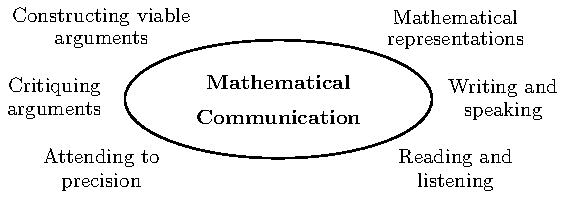
\includegraphics[width=0.6\linewidth]{tikz/communication} 

}

\caption{Components of Mathematical Communication}\label{fig:communication}
\end{figure}

All types of communication require a language. Within a language there exists a shared meaning behind the words and symbols used when communicating with a particular language. Mathematics communication, in this sense, operates much as a language does. However, unlike a language such as English, mathematics is represented using a mixture of words that have very precise definitions and symbols that compress many different ideas and meanings into a very small amount of space (linguists call mathematics a ``dense'' language because of this property). Moreover, somewhat uniquely to mathematics, the meaning of symbols varies widely depending upon the context of the communication. Consider variables, which are usually represented using any number of symbols. While certain types of symbols will cue a well-informed mathematics student that a variable has some implied meaning in terms of what type of number system to which it belongs, even in this case variables in different circumstances serve different roles. Sometimes the letter represents a fixed value (e.g., \(x=4\)) and other times it represents a range of values that satisfy a particular condition (e.g., \(x\leq 4\)). Sometimes it indexes a set, while other times it represents a function. The differences between these uses are often subtle, making explicit training in these nuances mathematics critical.

Once the language of mathematics has been developed, the grammar is created. In mathematics, logic, argument, and proof form the core patterns of organization and presentation. Together, logic, argument, and proof boil down to the ability to construct viable arguments and critique the arguments of others using mathematical evidence.

Part of mathematical communication is learning how to consume and understand the ideas of others. In mathematics this usually occurs by reading or listening to the arguments of others. Both reading and listening to mathematics require a great deal of practice and are skills students must hone over many courses. In particular, reading mathematics requires a great deal of practice and discipline. While a novel can usually be consumed at a steady pace without much explicit effort by the reader, written mathematical ideas are often presented symbolically, with the reader left to fill in certain logical steps. Thus, the act of reading mathematics becomes one of translation of the symbolic work into a language he or she understands, followed by a effort to connect current parts of the argument to previously made points, and the absorption and evaluation of those ideas based on previous knowledge. As a result, reading mathematical texts and arguments requires a big investment in time. Sometimes it can take hours just to understand one line of a mathematical text! This slow, methodical way of reading is challenging to students of mathematics, but is a critical skill to develop as it is core to the practice of doing mathematics.

Previous paragraphs have described the difficulties and process of consuming mathematical texts. However, it is also important that students learn to produce their own mathematical communications in both oral and written forms. In communicating to others, it is essential that precise mathematical words are used, rather than slang, in order to reduce the confusion of potential readers. It is also useful to employ a variety of mathematical representations, including graphs, sketches, and diagrams to facilitate the communication of mathematical ideas.

As teachers of mathematics, we must continually emphasize the development of this practice of communicating mathematically by de-emphasizing simple answers to mathematical problems, teaching students how to read and write mathematics (not just about mathematics), and to promote classroom discourse to provide opportunities for students to experience different types of mathematical communication.

\hypertarget{understanding-mathematical-structures}{%
\subsection{Understanding Mathematical Structures}\label{understanding-mathematical-structures}}

While the definition of mathematics is not uniform or agreed on, most agree that mathematics is inherently about the study of underlying structures and logical reasoning. For example, the Encyclopædia Britannica \citeyearpar{definition} defines mathematics as ``the science of structure, order, and relation that has evolved from elemental practices of counting, measuring, and describing the shapes of objects.'' This means that an important practice in the doing of mathematics is to ``look for and make use of structure'' and to ``look for and express regularity in repeated reasoning'' \citep{CCSS}.

The pursuit and use of structure and regularity appear throughout all of mathematics. Mathematical structure informs every part of mathematics teaching, from instruction on common mathematical procedures to searching for and making connections between various, apparently unrelated, mathematical content areas to provide new insight into a problem. As teachers, we need to point out these mathematical structures to the students and help them learn how to discover the structures and regularity on their own.

\hypertarget{exercises-1}{%
\subsection{Exercises}\label{exercises-1}}

\begin{enumerate}
\def\labelenumi{\arabic{enumi}.}
\item
  Consider the following mathematical task:

  An electricity company charges Kelly \(\$0.15\) per kWh (kilowatt-hour) of electricity used, plus a basic connection charge of \(\$8.00\) per month. Find a function that helps Kelly estimate her monthly electricity bill for a given number of kWhs. Be explicit about the domain of the function you create.

  \begin{enumerate}
  \def\labelenumii{\alph{enumii})}
  \item
    NCTM emphasizes multiple representation of functions using verbal, tabular, graphical, and symbolic representations. Using this word problem as the verbal representation, express the function in each of the remaining ways.
  \item
    How does the ability to move between different representations of functions support students' development of the mathematical communication process standard?
  \item
    The problem solving section discussed the fact that a mathematical task is only considered a problem if the person working on the task does not know in advance a solution method that will produce a correct answer. Would you say that for part (a) you were engaged in mathematical problem solving as described in the standards? Why or why not?
  \item
    Under what conditions would the task be a problem for students you were teaching?
  \item
    Based on the description of mathematical modeling, would you say that finding the function for the task in part (a) represents mathematical modeling? Why or why not?
  \item
    A second part of the task asks students to estimate Kelly's electrical bill for the year, given that her monthly kWh usage ranges between 202 and 254 kWh.
  \item
    The textbook you got the problem from lists the answer to the extension as \(\$506.40\). What did the author do and what assumptions did she make in order to arrive at that answer? Do you agree with her process and assumptions? Why or why not?
  \item
    In arriving at your answer for part (a), would you say that you were engaged in mathematical problem solving? Why or why not?
  \item
    If you were using this task as a modeling activity for your students, what criteria would you use to evaluate whether their answer was reasonable?
  \end{enumerate}
\item
  There are five NCTM Process Standards and eight Common Core Standards for Mathematical Practice. While there is significant overlap between the two sets of standards, they are not the same. Read each set of standards. When there is overlap between the two sets of standards, create a map between them. Also identify the ways in which the two sets of standards differ. These regions are not at the heading level. You'll have to actually dig into the blurbs about each standard in their original documents.
\item
  A basic theorem that students use from an early age is that the sum of two even integers is even. A typical proof of this theorem might look something like this:

  Let \(a\) and \(b\) be even integers such that \(a=2m\) and \(b=2n\) where \(m\) and \(n\) are integers. Then \(a+b=2m+2n=2(m+n)\). Thus, the sum of two even integers is even.

  \begin{enumerate}
  \def\labelenumii{\alph{enumii})}
  \item
    The section on mathematical communication emphasizes the reliance of mathematical communication on precise definitions and symbols that compress complex ideas into short phrases. In examining this proof, identify the places where the problem statement or proof rely on a definition or compressed expression.
  \item
    Identify the places where the proof writer has left the reader to fill in logical steps or rationales.
  \item
    Rewrite the proof of the theorem without the use of any symbols, but with the same degree of precision and generalizability.
  \item
    In comparing the symbolic proof to your verbal proof, do you think it is easier to understand (i.e., more like a novel?) or do you think it would still be difficult to read if all mathematics were presented without symbols? Why or why not?
  \item
    If you reflect on the six parts of mathematical communication, which parts do you think you are best at? Which parts do you struggle the most with? What is one goal you have for yourself for mathematical communication that you want to develop during this course?
  \end{enumerate}
\end{enumerate}

\hypertarget{mathematics-content-standards-in-the-u.s.}{%
\section{Mathematics Content Standards in the U.S.}\label{mathematics-content-standards-in-the-u.s.}}

The current standards for mathematics and assessment in the United States are derived from a variety of sources and past initiatives. David Klein \citeyearpar{Klein2003} gives a good summary of the major events and influential individuals during the 20\textsuperscript{th} century. The current set of standards have origins to a pair of reports from the 1980's: one by NCTM \citeyearpar{NCTM1980}, \emph{An Agenda for Action}, and one by the U.S. National Commission on Excellence in Education \citeyearpar{NCEE1983}, \emph{A Nation at Risk}. Each provided a different view about what should occur to improve mathematics education in the United States. While these two documents were used as the basis for the `math wars' of the late 20\textsuperscript{th} century, the biggest difference between them is that the NCTM document focused primarily on standards for teaching methodologies, while \emph{A Nation at Risk} focused on standards of content knowledge.

The NCTM \citeyearpar{NCTM1980} recommended "that

\begin{enumerate}
\def\labelenumi{\arabic{enumi}.}
\item
  problem solving be the focus of school mathematics in the 1980s;
\item
  basic skills in mathematics be defined to encompass more than computational facility;
\item
  mathematics programs take full advantage of the power of calculators and computers at all grade levels;
\item
  stringent standards of both effectiveness and efficiency be applied to the teaching of mathematics;
\item
  the success of mathematics programs and student learning be evaluated by a wider range of measures than conventional testing;
\item
  more mathematics study be required for all students and a flexible curriculum with a greater range of options be designed to accommodate the diverse needs of the student population;
\item
  mathematics teachers demand of themselves and their colleagues a high level of professionalism;
\item
  public support for mathematics instruction be raised to a level commensurate with the importance of mathematical understanding to individuals and society" (p.~1).
\end{enumerate}

The National Commission on Excellence in Education \citeyearpar{NCEE1983} recommended that

\begin{itemize}
\item
  ``The teaching of \emph{mathematics} in high school should equip graduates to: (a) understand geometric and algebraic concepts; (b) understand elementary probability and statistics; (c) apply mathematics in everyday situations; and (d) estimate, approximate, measure, and test the accuracy of their calculations. In addition to the traditional sequence of studies available for college-bound students, new, equally demanding mathematics curricula need to be developed for those who do not plan to continue their formal education immediately'' (p.~25).
\item
  ``Standardized tests of achievement (not to be confused with aptitude tests) should be administered at major transition points from one level of schooling to another and particularly from high school to college or work. The purposes of these tests would be to: (a) certify the student's credentials; (b) identify the need for remedial intervention; and (c) identify the opportunity for advanced or accelerated work. The tests should be administered as part of a nationwide (but not Federal) system of State and local standardized tests. This system should include other diagnostic procedures that assist teachers and students to evaluate student progress'' (p.~28).
\item
  ``Persons preparing to teach should be required to meet high educational standards, to demonstrate an aptitude for teaching, and to demonstrate competence in an academic discipline. Colleges and universities offering teacher preparation programs should be judged by how well their graduates meet these criteria'' (p.~30).
\item
  ``Substantial nonschool personnel resources should be employed to help solve the immediate problem of the shortage of mathematics and science teachers. Qualified individuals including recent graduates with mathematics and science degrees, graduate students, and industrial and retired scientists could, with appropriate preparation, immediately begin teaching in these fields. A number of our leading science centers have the capacity to begin educating and retraining teachers immediately. Other areas of critical teacher need, such as English, must also be/addressed'' (p.~31).
\end{itemize}

NCTM followed it's 1980 report with the publication of the \textit{Curriculum and Evaluation Standards for School Mathematics} \citep{NCTM1989}. This document focused on the standards for teaching methodologies and mathematical practices. Content standards were sketched out, with overviews of the recommended content knowledge for students in 4-year grade bands. NCTM expanded this work with additional texts focusing on teaching standards and assessment: \textit{Professional Teaching Standards} (\citeyear{NCTM1991}) and \textit{Assessment Standards} (\citeyear{NCTM1995}). In 2000, NCTM released an updated version the 1989 standards with the \textit{Principles and Standards for School Mathematics} \citep{PSSM}. During this same time, many states developed more specific content standards reflecting the guidelines recommended by the 1989 document \citep{Raimi1998}. Although the NCTM document did not make content recomendations by specific grade levels, many of the state standards still resided at the grade-band level \citep[p. 677]{Reys2007}.

\hypertarget{common-core-state-standards-math}{%
\subsection{Common Core State Standards-Math}\label{common-core-state-standards-math}}

In 2002, Congress passed the No Child Left Behind Legislation. This bill required that states determine measurable content standards for each grade level and develop assessments based on these standards to be given to all students at specific grade levels (generally fourth, eighth, and twelfth grade) in order to receive federal school funding. Since each state developed their own standards, the level and specificity of these standards varied greatly between States \citep{Reys2007}.

It was in this environment that the National Governors Association Center for Best Practices and the Council of Chief State School Officers launched an effort in 2009 to develop ``a common core of internationally benchmarked standards in math and language arts for grades K-12'' \citep{CCSS}. These standards emphasize content knowledge, while also encouraging some of the teaching methodologies proposed by the NCTM documents.

In order to help teachers better understand how the topics in this book relate to the actual teaching and learning of their students, we include related content standards from the Common Core State Standards for Mathematics throughout the text. While not all states have adopted the Common Core State Standards for their school systems, these standards are a good representation of what is expected from students at different stages in their mathematical education.

\begin{quote}
\hypertarget{related-content-standards}{%
\subsubsection*{Related Content Standards}\label{related-content-standards}}
\addcontentsline{toc}{subsubsection}{Related Content Standards}

\begin{itemize}
\tightlist
\item
  (8.F.1) Understand that a function is a rule that assigns to each input exactly one output. The graph of a function is the set of ordered pairs consisting of an input and the corresponding output.
\item
  (HSF.IF.7) Graph functions expressed symbolically and show key features of the graph, by hand in simple cases and using technology for more complicated cases.
\end{itemize}
\end{quote}

Standards that align with the content of each section are provided in blocks with the title ``Related Content Standards.'' One such box is given above as an example. The sequence of numbers and letters proceeding each standard is its standardized abbreviation. The first part of the abbreviation identifies the grade band. Since the Common Core State Standards for high school do not have a recommended grade level for each of the standards, they are denoted by ``HS'' and the general area of mathematics. The second part of the abbreviation refers to the general domain of mathematics, and the third part refers to the location of the standard in that grade band and domain.

\hypertarget{nctm-caep-standards}{%
\subsection{NCTM-CAEP Standards}\label{nctm-caep-standards}}

Another requirement of the No Child Left Behind legislation was that states had to create standards for teachers to receive certification. These standards for certification needed to be measured with a blend of standardized assessments, portfolios, and coursework. As a result, certification in secondary mathematics in most states requires a major in mathematics (or its equivalent), the teaching of and about standards during certification coursework, and achievement of certain scores on a content specific standardized test (such as the PRAXIS). In addition, the NCTM partnered with the Council for the Accreditation of Educator Preparation (CAEP) to develop standards for what beginning secondary mathematics teachers should know and be able to do in the teaching of mathematics \citep{CAEP}.

The NCTM-CAEP content standards are built upon the standards developed by the Conference Board of Mathematical Sciences in \citeyearpar{MET1} and \citeyearpar{MET2}. The content of this book builds upon the contents of the first standard of ``Knowing and Understanding Mathematics''. In particular:

\begin{quote}
Candidates demonstrate and apply, with the incorporation of mathematics technology, conceptual understanding, procedural fluency, and factual knowledge of major mathematical domains: Number; Algebra and Functions; Statistics and Probability; Geometry, Trigonometry, and Measurement; Calculus; and Discrete Mathematics.
\end{quote}

We list the details of the NCTM-CAEP content standards below and discuss how this book connects to each of these standards.

\begin{quote}
\textbf{Essential Concepts in Number.} Candidates demonstrate and apply conceptual understanding, procedural fluency, and factual knowledge of number including flexibly applying procedures, using real and rational numbers in contexts, developing solution strategies, and evaluating the correctness of conclusions. Major mathematical concepts in Number include number theory; ratio, rate, and proportion; and structure, relationships, operations, and representations.
\end{quote}

Number systems are primarily covered in Chapters \ref{ch:number}, \ref{ch:group-1}, and \ref{ch:rings}. We introduce initial concepts of the number systems in Chapter \ref{ch:number}, focusing on operations and the basic properties of common number systems, including whole numbers, integers, rational, real, and complex numbers. Chapters \ref{ch:group-1} and \ref{ch:rings} expand these ideas through the added structure of rings and fields.

\begin{quote}
\textbf{Essential Concepts in Algebra and Functions.} Candidates demonstrate and apply understandings of major mathematics concepts, procedures, knowledge, and applications of algebra and functions including how mathematics can be used systematically to represent patterns and relationships including proportional reasoning, to analyze change, and to model everyday events and problems of life and society. Essential Concepts in Algebra and Functions include algebra that connects mathematical structure to symbolic, graphical, and tabular descriptions; connecting algebra to functions; and developing families of functions as a fundamental concept of mathematics. Additional Concepts should include algebra from a more theoretical approach including relationship between structures (e.g., groups, rings, and fields) as well as formal structures for number systems and numerical and symbolic calculations.
\end{quote}

Many of these concepts are spread throughout the text, as algebra and functions are fundamental to the secondary curriculum. That said, Chapters \ref{ch:function}, \ref{ch:group-1}, \ref{ch:rings}, and \ref{ch:real-valued-functions} specifically focus on topics of particular importance in understanding algebra and functions. In particular Chapter \ref{ch:real-valued-functions} combines the themes of the earlier chapters together using real-valued functions.

\begin{quote}
\textbf{Essential Concepts in Calculus.} Candidates demonstrate and apply understandings of major mathematics concepts, procedures, knowledge, and applications of calculus including the mathematical study of the calculation of instantaneous rates of change and the summation of infinitely many small factors to determine some whole. Essential Concepts in Calculus include limits; continuity; the Fundamental Theorem of Calculus; and the meaning and techniques of differentiation and integration.
\end{quote}

The essential concepts in calculus are currently excluded from this text with the understanding that most pre-service teachers are already required to take at least two semesters worth of calculus courses that focus on this content standard.

\begin{quote}
\textbf{Essential Concepts in Statistics and Probability.} Candidates demonstrate and apply understandings of statistical thinking and the major concepts, procedures, knowledge, and applications of statistics and probability including how statistical problem solving and decision making depend on understanding, explaining, and quantifying the variability in a set of data to make decisions. They understand the role of randomization and chance in determining the probability of events. Essential Concepts in Statistics and Probability include quantitative literacy; visualizing and summarizing data; statistical inference; probability; and applied problems.
\end{quote}

The essential concepts of statistics and probability are the focus of Part IV of the text, Data Analysis. In that section we focus on statistics and a study of variability, looking at different ways to measure, communicate, and understand variability in the context of statistical problems.

\begin{quote}
\textbf{Essential Concepts in Geometry, Trigonometry, and Measurement.} Candidates demonstrate and apply understandings of major mathematics concepts, procedures, knowledge, and applications of geometry including using visual representations for numerical functions and relations, data and statistics, and networks, to provide a lens for solving problems in the physical world. Essential Concepts in Geometry, Trigonometry, and Measurement include transformations; geometric arguments; reasoning and proof; applied problems; and non-Euclidean geometries.
\end{quote}

Part III on Geometry looks at the subject of Geometry from the perspectives of constructional, transformational, analytic, and algebraic. Each perspective helps us to better understand the essential concepts in geometry, trigonometry, and measurement, along with the interactions between geometry, algebra, functions, and number systems.

\hypertarget{exercises-2}{%
\subsection{Exercises}\label{exercises-2}}

\begin{enumerate}
\def\labelenumi{\arabic{enumi}.}
\item
  Reflect on your K-12 mathematics education. Based on the brief history described, what documents were being used to guide your curriculum?
\item
  Those who study mathematics curriculum describe the changing focus of what is written in school standards for mathematics as a pendulum. Over time, the pendulum swings between a focus on procedural fluency such as \emph{A Nation at Risk} \citeyearpar{NCEE1983} describes and the more process oriented standards as outlined by NCTM (1989).

  \begin{enumerate}
  \def\labelenumii{\alph{enumii})}
  \tightlist
  \item
    How does the Common Core State Standards attempt to unify the two extremes of the pendulum swing?
  \item
    How does treating the process standards as separate from the content standards provide an opportunity to continue to let the pendulum swing?
  \item
    Regardless of which documents were currently in vogue while you were in school, do you think your mathematics education was more procedurally focused or more process standard focused?
  \item
    Is how you were taught what you hope your own teaching will be like? Why or why not?
  \item
    K-12 mathematics students often think that mathematics is a set of unrelated procedures that they have to memorize how to do. In contrast, people who do mathematics for a living think mathematics is a conceptual and logical system where everything fits together. As you currently understand them, do you think the Common Core State Standards could support students in moving from thinking about mathematics as a set of unrelated procedures to a more conceptual system? Why or why not?
  \end{enumerate}
\end{enumerate}

\hypertarget{ch:sets}{%
\chapter{Set Theory}\label{ch:sets}}

In the mid-1800s the field of mathematics went through a major shift that ended up changing the very definition of mathematics. In 1847, George Boole wrote in the introduction to \emph{The Mathematical Analysis of Logic} that up to that point, ``the abstractions of the modern Analysis, not less than the ostensive diagrams of the ancient Geometry, have encouraged the notion, that Mathematics are essentially, as well as actually, the Science of Magnitude'' \citep{Boole}. Instead, Boole proposed a new definition, suggesting

\begin{quote}
We might justly assign it as the definitive character of a true Calculus, that it is a method resting upon the employment of Symbols, whose laws of combination are known and general, and whose results admit of a consistent interpretation\ldots{} It is upon the foundation of this general principle, that I purpose to establish the Calculus of Logic, and that I claim for it a place among the acknowledged forms of Mathematical Analysis, regardless that in its object and in its instruments it must at present stand alone.
\end{quote}

\begin{figure}

{\centering \includegraphics[width=0.35\linewidth]{images/Portrait_of_George_Boole} 

}

\caption{George Boole}\label{fig:unnamed-chunk-4}
\end{figure}

At the time that Boole wrote the above passage, mathematics as a field shifted from the study of quantities to the study of abstract structures based on logic and set theory. This change in the definition of mathematics freed up those who studied it to move beyond structures tied to physical interpretations and applications and move to a more abstract field. The abstractification of mathematics was a powerful moment, resulting in the development of fields such as quantum mechanics, relativity, cryptography, statistics.

In this chapter we will go through some of the basics of set theory needed to understand some of the later material and to develop a common vocabulary and set of notations. We do not offer a deep treatment of set theory as there are many textbooks, specifically in the area of Discrete Math, with a more detailed coverage of it.

\hypertarget{sets-and-subsets}{%
\section{Sets and Subsets}\label{sets-and-subsets}}

The foundation of modern mathematics is the theory of sets. Informally, sets can be thought of as collections of objects. While \textbf{set theory} is not specifically outlined in the content standards of most states, it is mentioned in the Common Core standards. The first reference to set theory occurs in the Introduction to Kindergarten, stating:

\begin{quote}
Students use numbers, including written numerals, to represent quantities and to solve quantitative problems, such as counting objects in a set; counting out a given number of objects; comparing sets or numerals; and modeling simple joining and separating situations with sets of objects, or eventually with equations such as \(5 + 2 = 7\) and \(7 - 2 = 5\). (Kindergarten students should see addition and subtraction equations, and student writing of equations in kindergarten is encouraged, but it is not required.) Students choose, combine, and apply effective strategies for answering quantitative questions, including quickly recognizing the cardinalities of small sets of objects, counting and producing sets of given sizes, counting the number of objects in combined sets, or counting the number of objects that remain in a set after some are taken away. \citep{CCSS}
\end{quote}

Set theory also makes an appearance in the high school standards related to counting and probability, as knowledge of sets is critical to understanding basic formulas in probability.

\begin{quote}
\hypertarget{related-content-standards-1}{%
\subsubsection*{Related Content Standards}\label{related-content-standards-1}}
\addcontentsline{toc}{subsubsection}{Related Content Standards}

\begin{itemize}
\tightlist
\item
  (HSS.CP.1) Describe events as subsets of a sample space (the set of outcomes) using characteristics (or categories) of the outcomes, or as unions, intersections, or complements of other events (``or,'' ``and,'' ``not'').
\end{itemize}
\end{quote}

We start our exploration of set theory by developing some basic notation and definitions. \citet{Cantor} defined sets in the following way.

\begin{quote}
Unter einer `Menge' verstehen wir jede Zusammenfassung \(M\) von bestimmten wohlunterschiedenen Objecten \(m\) unsrer Anschauung oder unseres Denkens (welche die `Elemente' von \(M\) genannt werden) zu einem Ganzen. (p.~481)

By a `Set' we mean each collection \(M\) of certain well-differentiated objects \(m\) of our perception or our thinking (which are called the `elements' of \(M\)) as a whole. (English translation)
\end{quote}

This definition proved to not be precise enough to avoid certain paradoxes.

\begin{example}[Russell's Paradox]
\protect\hypertarget{exm:unnamed-chunk-5}{}{\label{exm:unnamed-chunk-5} \iffalse (Russell's Paradox) \fi{} } Let \(R= \left\{ x \middle \vert x\notin x\right\}\), the set that contains all sets that are not members of themselves. Is \(R\) an element of \(R\)? If it is, then it is a set that is an element of itself and so could not be an element of \(R\), by its definition, thus leading to a contradiction. On the other hand, if one assumes that \(R\) is not an element of itself, then it satisfies the conditions of being an element of \(R\), also leading to a contradiction. Thus defining the paradox.
\end{example}

Even though Cantor's definition of a set leads to such paradoxes, we will use it as our working definition, with the detailed definition of set being a primitive notion in Zermelo-Fraenkel set theory. The Zermelo-Fraenkel axioms, combined with the axiom of choice, create the ZFC axioms upon which mathematics is built. Due to the level of abstraction involved in the axioms, we will not include a systematic coverage of the axioms in this text, but will reference them as needed.

\begin{definition}
\protect\hypertarget{def:unnamed-chunk-6}{}{\label{def:unnamed-chunk-6} }

\begin{itemize}
\item
  We will define a set by the collection of elements which belong to the set.
\item
  If \(A\) is a set and \(a\) is an object that belongs to \(A\), we say that \(a\) is an \textbf{element} of \(A\) and denote it as \(a\in A\).
\item
  If an object \(a\) is not an element of a set \(A\), we denote that by \(a \notin A\).
\item
  Let \(A\) and \(B\) be sets. We say that \(A=B\) if and only if every element of \(A\) is an element of \(B\) and every element of \(B\) is an element of \(A\). (In the ZFC axioms, this is referred to as the axiom of extensionality.)
\end{itemize}
\end{definition}

While the elements of a set are often written in a specific order, i.e.~\(\{1,2,3\}\), the members of a set have no particular order and the same set could be written as \(\{3, 1, 2, 1\}\), with the repetition being irrelevant since the set is defined by its elements.

We also need to note that \(a\) and \(\{a\}\) are two different mathematical objects (one is the element \(a\) and the other is the set that contains the element \(a\)). So \(A = \{a, \{a\}\}\) defines a set with two distinct elements: \(a\) and \(\{a\}\). Likewise, if \(B=\{1, 2, 3, \{4\}, 5\}\), then \(4\notin B\) but \(\{4\}\in B\). So the symbol \(4\) is not an element of \(B\), but the symbol \(\{4\}\) (the set that contains the element \(4\)) does belong to \(B\). These nuances mean that we have to be very careful with our notation and how we read the mathematical symbols.

Another way to describe sets is using set-builder notation. In this notation, we describe our new set using larger sets and a set of restrictions on (or description of) which objects in the larger set we are choosing to include. For instance, we can define \(C\) to be the set of all real numbers (denoted \(\mathbb{R}\)) greater than or equal to \(3\). In this case, the larger set is the set of real numbers and the condition that the numbers are greater than or equal to three is the restriction or description. Of course we do not want to have to keep writing so much down, so we create a short-hand way of defining this set:
\[ C = \left\{ x\in \mathbb{R} \middle \vert x\geq 3\right\}\] where the \(\vert\) separates the description of the larger set and the description of the restrictions. This notation is read ``\(C\) is the set of all of the elements \(x\) in the real numbers such that \(x\) is greater than or equal to 3.'' This set-builder notation is particularly useful when describing sets with more than just a few elements.

When sets are subsets of the real numbers, we can also describe them using interval notation. For the set \(C\) defined above, we can also write
\[C=[3,\infty)\] where the closed bracket, \([\), denotes that the endpoint is contained in the set, while an open bracket, \((\), denotes that the endpoint is not contained in the set. For real numbers \(a\) and \(b\), with \(a<b\), we have the following options as intervals from \(a\) to \(b\):
\[ (a,b) \quad (a,b] \quad [a,b) \quad [a,b] .\]

Once we have created notation for sets with a few elements and a large number of elements, we can describe how to denote a set without any elements.

\begin{definition}
\protect\hypertarget{def:unnamed-chunk-7}{}{\label{def:unnamed-chunk-7} } The set that does not contain any elements is called the \textbf{empty set} and is denoted by \(\emptyset\). Any set that contains at least one element is then called \textbf{non-empty}.
\end{definition}

In addition to determining how to describe sets, we must have a way to determine if two sets are the same or distinct.

A direct consequence of this definition is that the number of times an element is listed and the order of the elements is irrelevant for equality of sets. So \(\{a, b, c, d\}=\{b, a, c, c, d, b\}\) and \(\{1, 2\} \neq \{1, 2, 3\}\).

\begin{definition}
\protect\hypertarget{def:subset}{}{\label{def:subset} } Let \(A\) and \(B\) be sets. We say that \(A\) is a subset of \(B\), denoted \(A \subseteq B\), if every element of \(A\) is also an element of \(B\). If \(A\) is not a subset of \(B\), we sometimes denote this by \(A\nsubseteq B\). If there are elements of \(A\) is a subset of \(B\) and there are elements of \(B\) that are not contained in \(A\), then we say that \(A\) is a \textbf{proper subset} of \(B\) and denote it by \(A\subset B\).
\end{definition}

For example:
\[\{6, 7 \} \subseteq \{5, 6, 7, 8\},\]
\[\{x\in \mathbb{R} \vert x>5\} \subseteq \{x\in \mathbb{R} \vert x \geq 2\}, \mbox{ and }\]
\[ \{a,b,c\} \subseteq \{a,b,c\}. \]
Notice that the first two examples are proper subsets.

It is important to distinguish between the phrases `element of' and `contained in' when discussing sets. If \(A= \{a,b,c\}\), then we say that \(a\) is an element of \(A\), while \(\{a\}\) is contained in \(A\)

Since the empty set has no elements, it is by default a subset of every set. Similarly, every set is a subset of itself.

\begin{example}
\protect\hypertarget{exm:unnamed-chunk-8}{}{\label{exm:unnamed-chunk-8} } If \(A=\{a,b,c\}\) we can describe all of the subsets of \(A\),
\[ \emptyset, \{a\}, \{b\}, \{c\}, \{a,b\}, \{a,c\}, \{b,c\}, \{a, b, c\}.\]
This set of subsets of \(A\) is called the \textbf{power set} of \(A\) and denoted by \(\mathcal{P}(A)\).
\end{example}

We often need to prove that two sets are equal to one another, and we do not have the elements of the set listed out. In these situations the following theorem often proves useful.

\begin{theorem}
\protect\hypertarget{thm:set-equality}{}{\label{thm:set-equality} }Let \(A\) and \(B\) be sets. \(A=B\) if and only if \(A \subseteq B\) and \(B \subseteq A\).
\end{theorem}

\begin{proof}
\iffalse{} {Proof. } \fi{}Since the statement of the theorem is an `if and only if' statement, there are actually two components that need to be proven. We need to first prove that if \(A=B\) then \(A \subseteq B\) and \(B \subseteq A\). The second statement that needs proving is the converse: having \(A \subseteq B\) and \(B \subseteq A\) implies that \(A=B\). We will complete both arguments using the corresponding definitions.

Assume that \(A=B\). Then the definition of set equality states that every element of \(A\) is an element of \(B\). This means that \(A\) meets the definition of a subset of \(B\). That is: \(A\subseteq B\). In addition, the assumption that \(A=B\) gives us that every element of \(B\) is an element of \(A\). As a result, \(B\subseteq A\). Thus \[A=B \Rightarrow A\subseteq B \mbox{ and } B\subseteq A.\]

To prove the converse statement, we assume that \(A \subseteq B\) and \(B \subseteq A\). Thus, we have that every element of \(A\) is also an element of \(B\) and every element of \(B\) is also an element of \(A\). This is the definition of set equality and so we have that \(A=B\).

We have therefore proven both implications, and thus the theorem is proven.
\end{proof}

\hypertarget{venn-diagrams}{%
\subsection{Venn Diagrams}\label{venn-diagrams}}

In order to better understand relationships between subsets of a larger set, it is sometimes helpful to represent the relationships with a \textbf{Venn diagram}. In these diagrams, we use circle-like figures to represent sets, with everything inside the circle being inside of the set and everything outside of the circle being outside of the set.

\begin{example}
\protect\hypertarget{exm:unnamed-chunk-10}{}{\label{exm:unnamed-chunk-10} } Let \(A=\{2, 4, 6, 8, 10\}\) and \(B=\{3, 6, 9\}\). Then these sets could be represented by a Venn diagram such as the one below.
\end{example}
\begin{figure}

{\centering 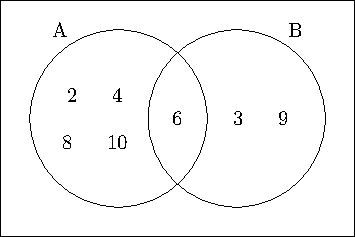
\includegraphics[width=0.35\linewidth]{tikz/VennEx2-1-6} 

}

\end{figure}

As previously discussed, sets do not have to just be composed of numbers. Moreover, sets can have many different relationships between them, as seen in Figure \ref{fig:venn-samples}. If a set is a subset of a second set, then they are visualized as one region inside of the other region. If there are elements shared between two sets, but are not known to have a subset relationship, then they are visualized as overlapping regions. If no elements of the two sets are the same, then they are represented as two non-overlapping regions. In the next section we define vocabulary to describe these different types of relationships and how they are combined in different ways.

\begin{figure}

{\centering 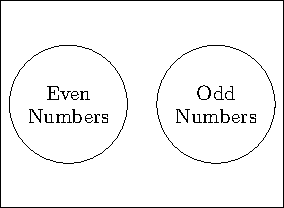
\includegraphics[width=0.3\linewidth]{tikz/evenodd} 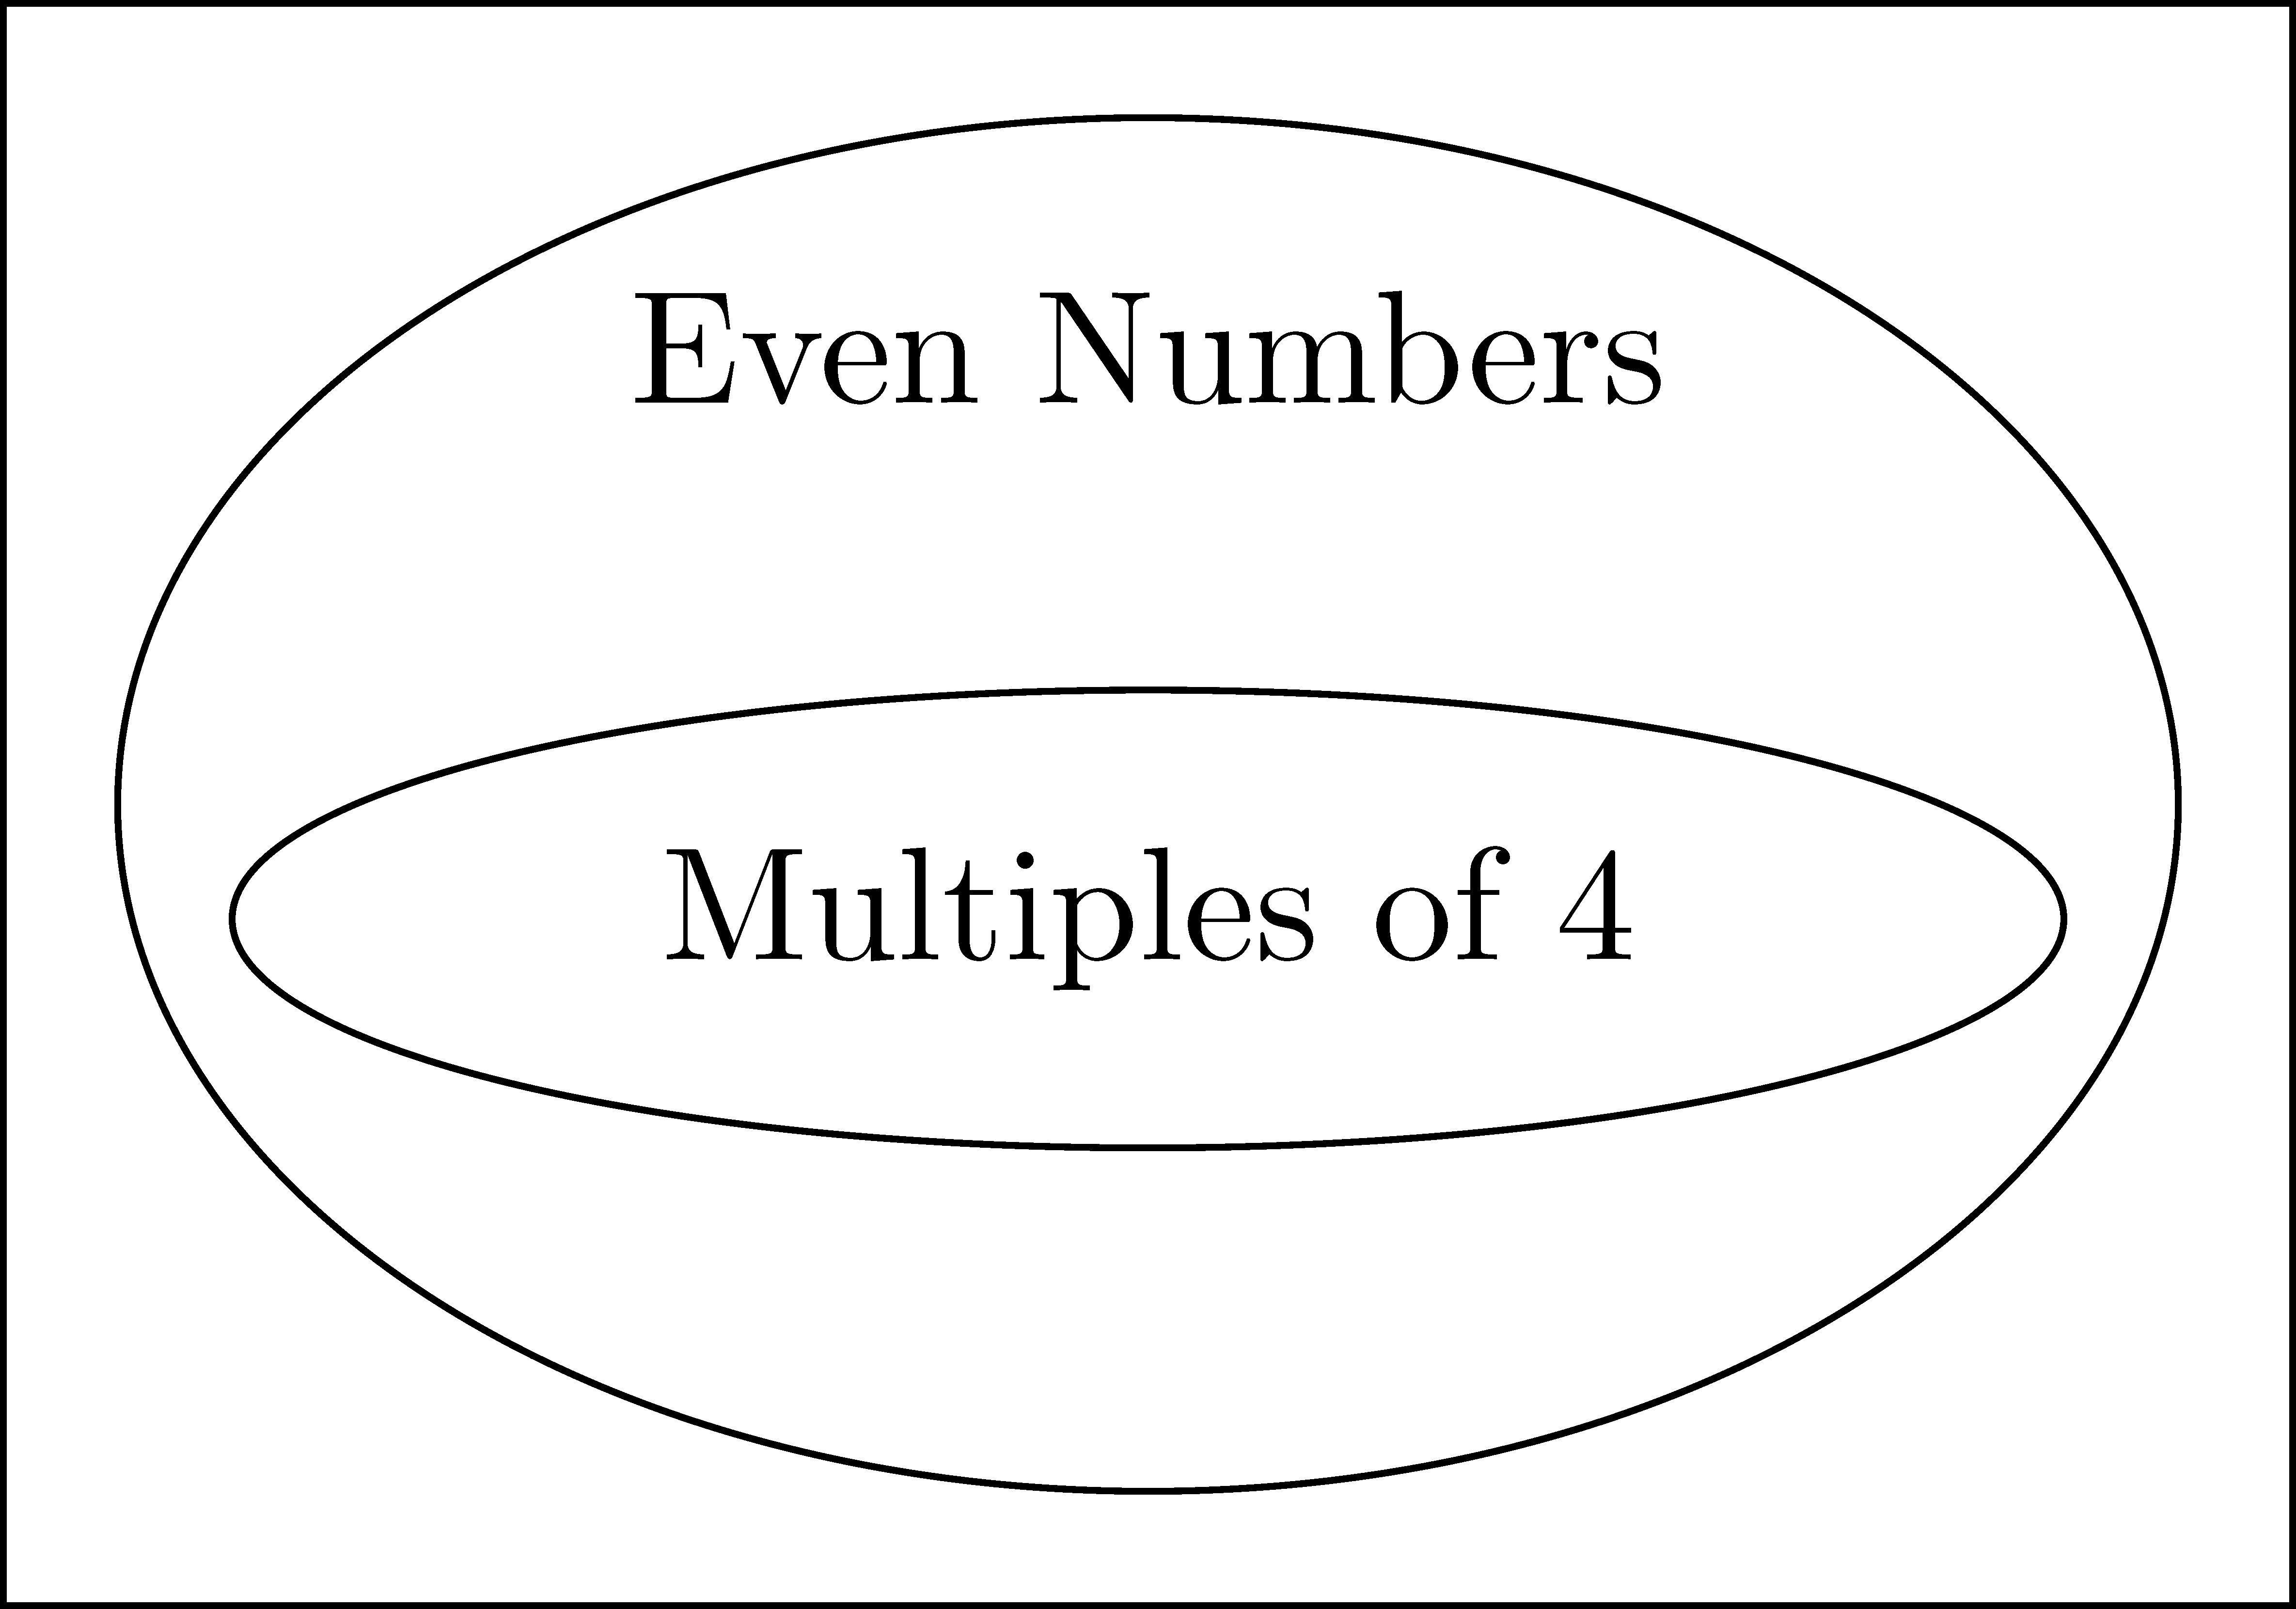
\includegraphics[width=0.3\linewidth]{tikz/evenfours} 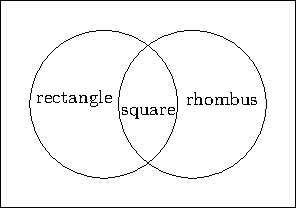
\includegraphics[width=0.3\linewidth]{tikz/rectsqrhombus} 

}

\caption{Sample Venn diagrams}\label{fig:venn-samples}
\end{figure}

\hypertarget{list-of-sets-of-numbers}{%
\subsection{List of Sets of Numbers}\label{list-of-sets-of-numbers}}

In order to help with terminology we will provide some notation for some of the basic sets used in the text.

We define the natural numbers as
\[\mathbb{N}=\{0,1,2,3,4,5,\ldots\}.\]
This is distinct from some definitions of the natural numbers that do not include the number \(0\). When a text defines the natural numbers without the \(0\), it also defines the whole numbers to be our definition of the natural numbers. We are including \(0\) due to the method in which we define the natural numbers in Chapter \ref{ch:number}.

We label the integers as \[\mathbb{Z} = \{\ldots, -4, -3, -2, -1, 0, 1, 2, 3, 4, \ldots\},\] which we will define in detail in Section \ref{sec:Integers}.

We label the set of rational numbers as \(\mathbb{Q}\) and the real numbers as \(\mathbb{R}\), the detailed definitions of which are in Sections \ref{sec:rationals} and \ref{sec:reals}, respectively.

The complex numbers, \(\mathbb{C}\), are defined and studied in Section \ref{sec:complex}.

For the integers, rationals and reals, we define \(\mathbb{Z}^+\), \(\mathbb{Q}^+\), and \(\mathbb{R}^+\) to be the positive elements of the set, those that are greater than zero.

We visualize the nested nature of these number systems in the Venn diagram in Figure \ref{fig:venn-numbers}.

\begin{figure}

{\centering 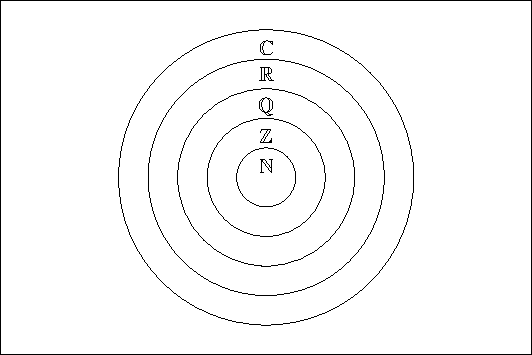
\includegraphics[width=0.7\linewidth]{tikz/vennNumberSystems} 

}

\caption{Sample Venn diagrams}\label{fig:venn-numbers}
\end{figure}

\hypertarget{exercises-3}{%
\subsection{Exercises}\label{exercises-3}}

\begin{enumerate}
\def\labelenumi{\arabic{enumi}.}
\item
  Answer the following as true or false. If false, explain why the statement is not true.

  \begin{enumerate}
  \def\labelenumii{\alph{enumii}.}
  \item
    \(\emptyset \subseteq \{f,u,n,t,i,m,e,s\}\)
  \item
    \(\{a,b\} \in \{a,b,c\}\)
  \item
    \(\{0 \}\ = \emptyset\)
  \item
    \(\{f,u,n,f,u,n \}=\{f,u,n \}\)
  \item
    \(\{0,0\} \subseteq \{0,0,1,1,2,2\}\)
  \end{enumerate}
\item
  Let \(A=\{1, 2, 3\}\), \(B=\{a, b, c\}\), and \(C=\{1, a, 2, b, 3, c\}\). Answer the following as true or false. If false, explain why the statement is not true.

  \begin{enumerate}
  \def\labelenumii{\alph{enumii})}
  \item
    \(A \subseteq A\)
  \item
    \(A\supseteq C\)
  \item
    \(A=B\)
  \item
    \(A \nsubseteq B\)
  \end{enumerate}
\item
  Recall that for set \(A\), \(\mathcal{P}(A)\) is the power set of \(A\).

  \begin{enumerate}
  \def\labelenumii{\alph{enumii})}
  \item
    Let \(A=\{a,b\}\). Write the set of \(\mathcal{P}(A)\) by listing its elements.
  \item
    Let \(A\) be a set with \(n\) elements in it.
  \item
    How many elements are in \(\mathcal{P}(A)\) if \(n=3\)?
  \item
    How many elements are in \(\mathcal{P}(A)\) if \(n=4\)?
  \item
    How many elements are in \(\mathcal{P}(A)\) if \(n\) is an unknown natural number?
  \end{enumerate}
\item
  Some textbooks describe a set as ``a well-defined collection of objects'' which means that the inclusion criteria that helps you decide what should be in the set is clearly specified. Classify each of the following sets as well-defined or not. If you identify a set as not well-defined, give two possible well-defined sets that would satisfy the original description.

  \begin{enumerate}
  \def\labelenumii{\alph{enumii})}
  \item
    \(\{x \vert x>0\}\)
  \item
    The set of students at The University of Awesome who are currently enrolled in a class that has a 100-level designation.
  \item
    \(\{x\vert x \textrm{ is a letter in my first name}\}\)
  \item
    The set of my friends.
  \item
    \(A_n=\{x\in \mathbb{Z} \vert n\leq x\leq n+3\}\)
  \end{enumerate}
\item
  Let \(A=\{1, 2, 3, 4\}\), \(B=\{7,8,9\}\), and \(C=\{3,4,5,6,7,8,9\}\). Using the most appropriate template of the Venn diagrams shown in Figure \ref{fig:venn-samples}, fill in the regions with the elements from:

  \begin{enumerate}
  \def\labelenumii{\alph{enumii})}
  \item
    Sets \(A\) and \(B\).
  \item
    Sets \(A\) and \(C\).
  \item
    Sets \(B\) and \(C\).
  \item
    Sets \(A\), \(B\), and \(C\) (you will have to make a new Venn diagram template).
  \end{enumerate}
\end{enumerate}

\hypertarget{algebra-of-sets}{%
\section{Algebra of Sets}\label{algebra-of-sets}}

Now that we understand the basic definitions involving sets, we examine set operations. These will allow us to create new sets from given sets.

\begin{definition}
\protect\hypertarget{def:unnamed-chunk-12}{}{\label{def:unnamed-chunk-12} }Let \(A\) and \(B\) be sets. We define the union of \(A\) and \(B\), denoted \(A \cup B\), to be the set of elements that are either in \(A\) or \(B\), or possibly both. We define the intersection of \(A\) and \(B\), \(A \cap B\), to be the set of elements that are in both \(A\) and \(B\). We say that \(A\) and \(B\) are \textbf{disjoint} if \(A\cap B = \emptyset\).
\end{definition}

The shaded regions in Figure \ref{fig:set-union} illustrate each set relationship in terms of general sets \(A\) and \(B\). We can also write the union and intersection of sets in terms of set-builder notation:
\[A\cup B = \{x \vert x\in A \mbox{ or } x\in B\} \quad \mbox{ and } \quad A\cap B =\{x\vert x\in A \mbox{ and } x\in B\}.\]

\begin{figure}

{\centering 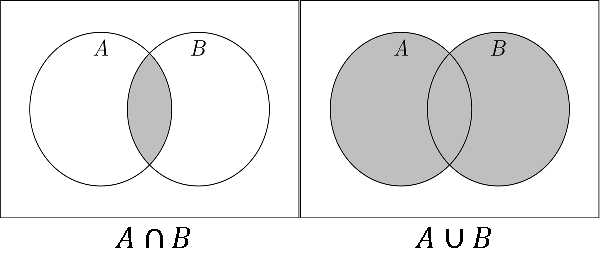
\includegraphics[width=0.7\linewidth]{tikz/Set_unions_intersections} 

}

\caption{The union and intersection of two sets}\label{fig:set-union}
\end{figure}

Let's look at a couple of examples to better understand these unions and intersections.

\begin{example}
\protect\hypertarget{exm:unnamed-chunk-13}{}{\label{exm:unnamed-chunk-13} } Let \(A = \{a, b, c, d, e\}\) and \(B = \{ d, e, f, g\}\). Then \[A\cup B=\{a, b, c, d, e, f, g\} \]
\end{example}

\begin{example}
\protect\hypertarget{exm:unnamed-chunk-14}{}{\label{exm:unnamed-chunk-14} } Let \(A=\{1,2,3,4,5,6,7,8,9\}\) and \(B=\{2,4,6,8\}\). Then
\[A \cup B = A \quad \mbox{ and } \quad A\cap B = B.\]
\end{example}

\begin{example}
\protect\hypertarget{exm:unnamed-chunk-15}{}{\label{exm:unnamed-chunk-15} } Let \(A=\{a,b,c\}\) and \(B=\{1,2,3\}\). Then
\[A\cup B = \{a,b,c,1,2,3\} \quad \mbox{ and } \quad A\cap B =\emptyset.\]
\end{example}

\begin{example}
\protect\hypertarget{exm:unnamed-chunk-16}{}{\label{exm:unnamed-chunk-16} } Let \(A = \{ x\in \mathbb{R} \: \vert \: x > 5\}\) and \(B=\{x \in \mathbb{R} \: \vert \: x < 8\}\). Then \(A\cup B\) would be all real numbers, since any real number is either less than 8 or greater than 5. And \(A\cap B\) would be the real numbers between 5 and 8. These can also be represented on number lines, where the shaded lines and filled dots are included in the set, with open dots and unshaded lines not being included in the set.
\end{example}

\begin{center}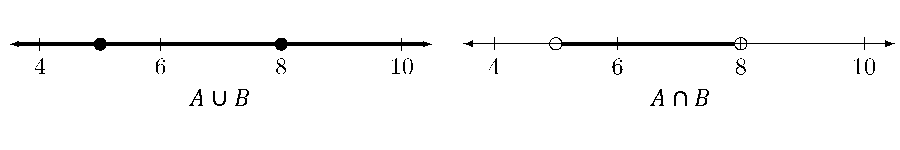
\includegraphics[width=0.95\linewidth]{tikz/number-line-unions} \end{center}

The following theorem identifies properties of the union as an operation on sets that follow from the definition.

\begin{theorem}
\protect\hypertarget{thm:unnamed-chunk-18}{}{\label{thm:unnamed-chunk-18} }Let \(A\), \(B\), and \(C\) be sets. Then we have the following:

\begin{enumerate}
\def\labelenumi{\arabic{enumi}.}
\item
  \(A\cup \emptyset = A\)
\item
  \(A \cup A = A\)
\item
  \(A \cup B = B \cup A\)
\item
  \(A \cup (B\cup C ) = (A\cup B) \cup C\)
\item
  \(A \subseteq A \cup B\)
\item
  If \(A \subseteq B\), then \(A\cup B=B\)
\end{enumerate}
\end{theorem}

\begin{proof}
\iffalse{} {Proof. } \fi{}The first two statements follow directly from the definition of the union. The empty set has no elements, making its union with \(A\) equal to \(A\). Because \(A\) and \(A\) have the same elements, the union must also be \(A\).

The third statement suggests that the set operation ``union'' is commutative, in that the order of the operation does not matter. The proof follows from properties of symbolic logic in relation to the use of the ``or'' statement in the definition of the union.

The fourth statement in the theorem is used to expand the definition of union, which is only defined for a pair of sets, to more than two sets. A further consequence of statement four is that the method of pairing sets the under the operation of union is irrelevant. We show this by proving the two statements \(A \cup (B\cup C ) \subseteq (A\cup B) \cup C\) and \((A\cup B) \cup C \subseteq A \cup (B\cup C)\) (see Theorem \ref{thm:set-equality}). In order to show the first containment, we let \(x\in A \cup (B\cup C )\) be a generic element. Then by the definition of the union of sets, \(x\in A\) or \(x\in (B\cup C)\). We will then break this statement into two cases.

\textbf{Case 1.} If \(x\in A\), then by the definition of unions \(x\in (A \cup B)\). Then using the definitions of unions again, \(x \in ((A \cup B) \cup C)\).

\textbf{Case 2.} If \(x\in (B\cup C)\), then \(x\in B\) or \(x\in C\). If \(x\in B\), then \(x\in (A\cup B)\) and also \(x\in ((A\cup B) \cup C)\). If \(x\in C\), then \(x\in ((A\cup B) \cup C)\).

So in either case, \(x \in A \cup (B\cup C)\) implies that \(x\in (A\cup B) \cup C\). So \(A\cup (B\cup C) \subseteq (A\cup B)\cup C\). The proof of the reverse containment is nearly identical.

We leave the last two statements as exercises.
\end{proof}

Similar to the union, the following theorem demonstrates how the intersection of sets works as an operation on sets. The proofs for each statement are similar to that of the unions so we will leave the proof of this theorem as an exercise.

\begin{theorem}
\protect\hypertarget{thm:intersections}{}{\label{thm:intersections} }Let \(A\), \(B\), and \(C\) be sets. Then we have the following

\begin{enumerate}
\def\labelenumi{\arabic{enumi}.}
\item
  \(A\cap \emptyset = \emptyset\)
\item
  \(A \cap A = A\)
\item
  \(A \cap B = B \cap A\)
\item
  \(A \cap (B\cap C ) = (A\cap B) \cap C\)
\item
  If \(A \subseteq B\), then \(A \cap B = A\)
\end{enumerate}
\end{theorem}

Now that we know how unions and intersections behave by themselves, we examine how they interact with each other.

\begin{theorem}
\protect\hypertarget{thm:set-distribution}{}{\label{thm:set-distribution} }Let \(A\), \(B\), and \(C\) be sets. Then
\[ A \cap (B \cup C) = (A \cap B) \cup (A \cap C) \quad \mbox{ and } \quad  A \cup (B \cap C) = (A \cup B) \cap (A \cup C).\]
\end{theorem}

These relationships are diagrammed in Figure \ref{fig:set-distributions}.

\begin{figure}

{\centering 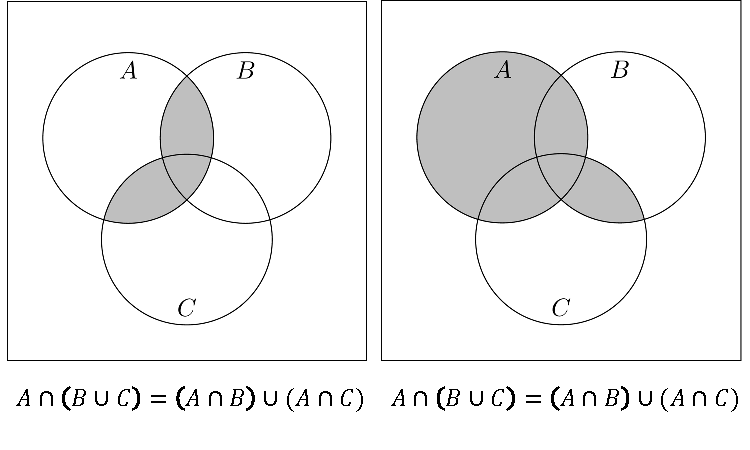
\includegraphics[width=0.8\linewidth]{tikz/set-distribution} 

}

\caption{Venn Diagrams for Set Distribuions }\label{fig:set-distributions}
\end{figure}

\begin{proof}
\iffalse{} {Proof. } \fi{} As each of these are proofs of equality of sets, we will need to complete the proofs showing that each set is contained in the other (see Theorem \ref{thm:set-equality}). We prove Part 1 and leave Part 2 as an exercise.

Let \(x\in A \cap (B \cup C)\). Then \(x\in A\) and \(x\in (B\cup C)\). This yields two cases: \(x\in A\) and \(x\in B\), or \(x\in A\) and \(x\in C\). This is equivalent to \(x \in (A\cap B) \cup (A\cap C)\). Thus \(A \cap (B \cup C) \subseteq (A \cap B) \cup (A \cap C)\).

If \(x\in (A \cap B) \cup (A \cap C)\), then we have to examine two cases: \(x\in (A\cap B)\) or \(x\in (A \cap C)\).

\textbf{Case 1.} If \(x\in (A\cap B)\), then \(x\in A\) and \(x\in B\). Since \(x\in B\), we know that \(x\in (B\cup C)\). Thus \(x\in A \cap (B\cup C)\).

\textbf{Case 2.} If \(x \in (A\cap C)\), then \(x\in A\) and \(x\in C\). Since \(x\in C\), we know that \(x \in (B\cup C)\). Thus \(x \in A \cap (B\cup C)\).

These results imply that \((A \cap B) \cup (A \cap C) \subseteq A \cap (B \cup C)\). Thus, the Part 1 of the theorem is proven.
\end{proof}

\hypertarget{set-complements}{%
\subsection{Set Complements}\label{set-complements}}

When working on a problem, we usually describe several sets, with an underlying assumption that the sets referenced contain elements from some common, larger set. We call a set that contains all of the elements considered for a particular situation a \textbf{universal set}.

\begin{definition}
\protect\hypertarget{def:unnamed-chunk-21}{}{\label{def:unnamed-chunk-21} }For every set \(A\) that is a subset of the universal set \(U\), we define the \textbf{complement} of \(A\) to be the set of elements in the universal set that are not in \(A\), denoted
\[A^c=\left\{ x\in U \middle \vert x \notin A\right\}.\]\\
\end{definition}

\begin{figure}

{\centering 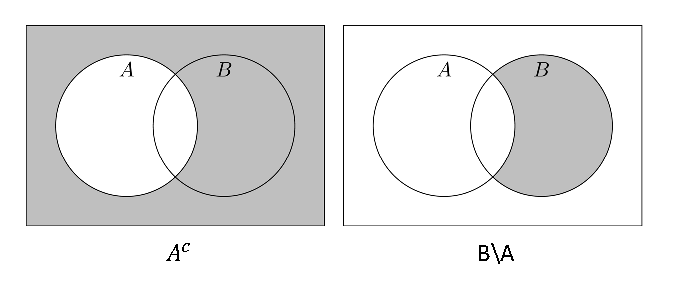
\includegraphics[width=0.8\linewidth]{tikz/set-difference} 

}

\caption{Set Complement and Set Difference}\label{fig:set-difference}
\end{figure}

For a given set \(A\) in universal set \(U\), the complement of a set identifies everything that is in the universal set except for things in set \(A\). This is often useful, however there are times when it is important to consider the elements that are in one set, but not in another, without reference to the universal set.

\begin{definition}
\protect\hypertarget{def:unnamed-chunk-22}{}{\label{def:unnamed-chunk-22} } Let \(A\) and \(B\) be sets. The complement of \(A\) with respect to \(B\), also called the \textbf{set difference} of \(B\) and \(A\), is defined as
\[B\setminus A = B \cap A^c = \left\{x\in B \middle \vert x \notin A\right\}.\]
\end{definition}

Let's revisit our previous examples to understand this idea of a set difference.

\begin{example}
\protect\hypertarget{exm:unnamed-chunk-23}{}{\label{exm:unnamed-chunk-23} } Let \(A = \{a, b, c, d, e\}\) and \(B = \{ d, e, f, g\}\). Then \[A\setminus B=\{a, b, c\} \quad \mbox{ and } \quad  B\setminus A =\{ f, g\}.\]
\end{example}

\begin{example}
\protect\hypertarget{exm:unnamed-chunk-24}{}{\label{exm:unnamed-chunk-24} } Let \(A=\{1,2,3,4,5,6,7,8,9\}\) and \(B=\{2,4,6,8\}\). Then
\[A \setminus B = \{1,3,5,7,9\} \quad \mbox{ and } \quad B\setminus A = \emptyset.\]
\end{example}

\begin{example}
\protect\hypertarget{exm:unnamed-chunk-25}{}{\label{exm:unnamed-chunk-25} } Let \(A=\{a,b,c\}\) and \(B=\{1,2,3\}\). Then
\[A\setminus B = A \quad \mbox{ and } \quad B\setminus A =B.\]
\end{example}

\hypertarget{de-morgans-laws}{%
\subsection{De Morgan's Laws}\label{de-morgans-laws}}

In the same year as the seminal work of Boole \citeyearpar{Boole} that started mathematics as a theoretical discipline, Augustus De Morgan published a foundational work in logic \citep{DeMorgan}. In this book, De Morgan defines and describes symbolic mathematical logic. His work has become the foundation for our current mathematical system. One of the key components of this work examines the complements of intersections and unions \citep[p.~69]{DeMorgan}.

\begin{theorem}[De Morgan's laws]
\protect\hypertarget{thm:unnamed-chunk-26}{}{\label{thm:unnamed-chunk-26} \iffalse (De Morgan's laws) \fi{} }If \(A\) and \(B\) are subsets of the same universal set, then
\[ \left(A \cap B\right)^c = A^c \cup B^c \quad \mbox{and} \quad \left(A \cup B \right)^c = A^c \cap B^c.\]
\end{theorem}

\begin{proof}
\iffalse{} {Proof. } \fi{} Because we are proving that two sets are equal we need to prove that the sets are subsets of each other. Here we will prove that \(\left(A \cap B\right)^c = A^c \cup B^c\) and leave the other proof as an exercise.

(Proof that \(\left(A \cap B\right)^c \subseteq A^c \cup B^c\).):

Let \(x\in \left(A \cap B\right)^c\). So \(x\) is not in \(A\cap B\). \(x\) is not in both \(A\) and \(B\).

Case 1. If \(x\in A\), then \(x\notin B\). So \(x\in B^c\).

Case 2. If \(x\notin A\), then \(x\in A^c\).

So either way, \(x\) is in \(A^c\) or \(x\) is in \(B^c\) (\(x\in A^c \cup B^c\)). Therefore, \(\left(A \cap B\right)^c \subseteq A^c \cup B^c\).

(Proof that \(A^c \cup B^c \subseteq \left(A \cap B\right)^c\).):

Let \(x \in A^c \cup B^c\).

Case 1. \(x\in A^c\). Then \(x\notin A\). So \(x\notin A\cap B\). So \(x\in (A\cap B)^c\).

Case 2. \(x\in B^c\). Then \(x\notin B\). So \(x\notin A\cap B\). So \(x\in A\cap B)^c\).

Therefore, \(A^c \cup B^c \subseteq \left(A \cap B\right)^c\)

Therefore, \(\left(A \cap B\right)^c = A^c \cup B^c\).
\end{proof}

It is also helpful to understand De Morgan's laws by looking at the corresponding Venn diagrams, shown in Figure \ref{fig:demorgan}.

\begin{figure}

{\centering 
\includegraphics[width=0.8\linewidth]{tikz/demorgan} 

}

\caption{Venn diagrams for De Morgan's laws for pairs of sets}\label{fig:demorgan}
\end{figure}

\hypertarget{subsec:cartesian}{%
\subsection{Cartesian Products}\label{subsec:cartesian}}

The previous sections have considered set operations between two sets that exist in the same universal set. Sets can also be combined to create new sets that exist in a universal set that differs from those of the sets used to create it. The collection of set operations that do this allows us to use sets to create multidimensional systems such as ordered pairs.

\begin{definition}
\protect\hypertarget{def:unnamed-chunk-28}{}{\label{def:unnamed-chunk-28} } The \textbf{Cartesian Product} of two non-empty sets \(A\) and \(B\) is the set
\[A\times B = \left\{ (a,b) \middle \vert a \in A, b\in B\right\}\] of all ordered pairs of elements where the first coordinate in the pair comes from the set \(A\) and the second coordinate is an element of \(B\).
\end{definition}

The most common Cartesian product in the secondary mathematics curriculum is real plane, \(\mathbb{R} \times \mathbb{R}\), which is often denoted by \[\mathbb{R}^2:= \left\{ (x,y) \vert x,y\in \mathbb{R} \right\}.\]

\begin{quote}
\hypertarget{related-content-standards-2}{%
\subsubsection*{Related Content Standards}\label{related-content-standards-2}}
\addcontentsline{toc}{subsubsection}{Related Content Standards}

\begin{itemize}
\tightlist
\item
  (5.G.1) Use a pair of perpendicular number lines, called axes, to define a coordinate system, with the intersection of the lines (the origin) arranged to coincide with the \(0\) on each line and a given point in the plane located by using an ordered pair of numbers, called its coordinates. Understand that the first number indicates how far to travel from the origin in the direction of one axis, and the second number indicates how far to travel in the direction of the second axis, with the convention that the names of the two axes and the coordinates correspond (e.g., \(x\)-axis and \(x\)-coordinate, \(y\)-axis and \(y\)-coordinate).
\end{itemize}
\end{quote}

The concept of the Cartesian product can be generalized to more than a pair of sets, for example \[\mathbb{R}^3:= \left\{ (x,y,z) \vert x,y,z\in \mathbb{R} \right\}\] is the three dimensional Cartesian space where each coordinate is a real number.

\begin{theorem}
\protect\hypertarget{thm:set-identities}{}{\label{thm:set-identities} }It is sometimes helpful to summarize all of the properties of algebra on sets into a single location.

Let all sets referred to below be subsets of a universal set \(U\).

\begin{enumerate}
\def\labelenumi{\arabic{enumi}.}
\item
  (Commutative Laws) For all sets \(A\) and \(B\),
  \[(a) \: A \cup B = B \cup A \quad \mbox{and} \quad (b) \: A \cap B = B \cap A\]
\item
  (Associative Laws) For all sets \(A\), \(B\), and \(C\),
  \[(a) \: (A\cup B)\cup C = A \cup (B \cup C) \quad \mbox{and} \quad (b) \: (A \cap B) \cap C = A \cap (B\cap C)\]
\item
  (Distributive Laws) For all sets \(A\), \(B\), and \(C\),
  \[(a) \: A \cup (B \cap C) = (A \cup B)\cap (A \cup C) \quad \mbox{and} \quad (b) \: A \cap (B \cup C) = (A \cap B)\cup (A \cap C)\]
\item
  (Identity Laws) For all sets \(A\),
  \[(a) \: A \cup \emptyset = A \quad \mbox{and} \quad (b) \: A \cap U = A\]
\item
  (Complement Laws)
  \[(a) \: A \cup A^c = U \quad \mbox{and} \quad (b) \: A \cap A^c = \emptyset\]
\item
  (Double Complement Law) For all sets \(A\),
  \[(A^c)^c =A\]
\item
  (Idempotent Laws) For all sets \(A\),
  \[(a) \: A\cup A=A \quad \mbox{and} \quad (b) \: A \cap A =A\]
\item
  (Universal Bound Laws) For all sets \(A\),
  \[(a) \: A \cup U = U\quad \mbox{and} \quad (b) \: A \cap \emptyset = \emptyset\]
\item
  (De Morgan's Laws) For all sets \(A\) and \(B\),
  \[(a) \: (A \cup B)^c = A^c \cap B^c\quad \mbox{and} \quad (b) \: (A \cap B)^c = A^c \cup B^c\]
\item
  (Absorption Laws) For all sets \(A\) and \(B\),
  \[(a) \: A \cup (A \cap B) = A \quad \mbox{and} \quad (b) \: A \cap (A \cup B ) = A\]
\item
  (Complements of \(U\) and \(\emptyset\))
  \[(a) \: U^c = \emptyset \quad \mbox{and} \quad (b) \: \emptyset^c = U\]
\item
  (Set Difference Law) For all sets \(A\) and \(B\),
  \[A\setminus B = A \cap B^c\]
\end{enumerate}
\end{theorem}

\hypertarget{exercises-4}{%
\subsection{Exercises}\label{exercises-4}}

\begin{enumerate}
\def\labelenumi{\arabic{enumi}.}
\item
  Middle and high school students often struggle to remember the difference between union and intersection.

  \begin{enumerate}
  \def\labelenumii{\alph{enumii})}
  \tightlist
  \item
    Describe a memory trick to help students remember which symbol goes with which of the two operations.
  \item
    Review the definitions of the intersection and union of two sets. What key words separate the two definitions from each other?
  \item
    Some students, when first learning the mathematical definition of union, think that the definition excludes objects that are in both sets. These students, when given two sets and asked to find \(A \cup B\) will include the items that are in \(A\) only and \(B\) only. They exclude things in \(A \cap B\). What might be the source of this misconception?
  \item
    Define a non-numeric universe and two sets, \(A\) and \(B\), in your universe such that \(A \cap B \neq \emptyset\). Describe, using words, each of the following sets:

    \begin{enumerate}
    \def\labelenumiii{\roman{enumiii}.}
    \tightlist
    \item
      \(A \cup B\)
    \item
      \(A \cap B\)
    \item
      \(A^{C}\)
    \end{enumerate}
  \end{enumerate}
\item
  Let \(A = \{1, 3, 5, 7, 9\}\), \(B=\{1, 2, 3, 4\}\), and \(C=\{3, 6, 9\}\). List the elements of each of the specified sets.

  \begin{enumerate}
  \def\labelenumii{\alph{enumii}.}
  \tightlist
  \item
    \(A \cap B\)
  \item
    \(A \cup B\)
  \item
    \(A \cup C\)
  \item
    \((A\cap B) \cup C\)
  \item
    \(A \cap (B \cup C)\)
  \item
    \(A \times B\)
  \item
    \(B \times (A\cap C)\)
  \end{enumerate}
\item
  For this exercise, assume that \(\mathbb{R}\) is the universal set. For any natural number, \(n\), define \(n\mathbb{Z} = \{nx \vert x \in \mathbb{Z}\}\). Answer the following as true or false. If false, explain why the statement is not true.

  \begin{enumerate}
  \def\labelenumii{\alph{enumii}.}
  \tightlist
  \item
    \((2\mathbb{Z})^C = \{2x+1 \vert x \in \mathbb{Z}\}\)
  \item
    \(\mathbb{R}\setminus \mathbb{Z}=\mathbb{Z}^C\)
  \item
    \(5\mathbb{Z} \cap \{2x+1 \vert x \in \mathbb{Z}\} = 5\mathbb{Z}\)
  \item
    \(5\mathbb{Z} \cap 4\mathbb{Z} = 20\mathbb{Z}\)
  \item
    \(2\mathbb{Z}\setminus (4\mathbb{Z} \cup 6\mathbb{Z})= \emptyset\)
  \item
    \(3\mathbb{Z}\setminus 2\mathbb{Z}=\{3(2x-1) \vert x\in \mathbb{Z} \textrm{ and } x\geq 0\}\)
  \end{enumerate}
\item
  Let \(A\) and \(B\) be sets. Prove that \(A\subseteq A\cup B\).
\item
  Let \(A\) and \(B\) be sets. Prove that if \(A\subseteq B\), then \(A\cup B=B\).
\item
  Prove Theorem \ref{thm:intersections}.
\item
  Prove Part 2 of Theorem \ref{thm:set-distribution}.
\item
  Prove that for sets \(A\) and \(B\), \((A\cap B)^c = A^c \cup B^c\) and \((A\cup B)^c=A^c\cap B^c\)
\item
  Write \((A\setminus B)\cup (B\setminus A)\) in terms of just unions, intersections, and complements, then simplify your expression.
\item
  Often when doing mathematics, the set you are working with or within is left unstated.

  \begin{enumerate}
  \def\labelenumii{\alph{enumii}.}
  \tightlist
  \item
    Under what conditions is it important to be explicit with students about the set you are working within?
  \item
    What set do you assume you are working in when:

    \begin{enumerate}
    \def\labelenumiii{\arabic{enumiii}.}
    \tightlist
    \item
      You are figuring out how much something will cost?
    \item
      You are figuring out what proportion of a pizza to give everyone?
    \item
      You are determining what the temperature will be if it is predicted to drop 20 degrees overnight?
    \end{enumerate}
  \end{enumerate}
\item
  Construct an algebraic proof for the given statement. Cite a property from Theorem \ref{thm:set-identities} for every step.
\end{enumerate}

\begin{quote}
For all sets \(A\) and \(B\), \[A \cup (B-A)= A \cup B\]
\end{quote}

\hypertarget{collections-of-sets}{%
\section{Collections of Sets}\label{collections-of-sets}}

Now that we know how to combine pairs of sets, we can inductively define unions and intersections for a finite or infinite number of sets.

When we are dealing with more than one or two related but distinct sets we often use another set as an \textbf{index set} in order to more easily describe and distinguish the sets in the collection.

\begin{example}
\protect\hypertarget{exm:unnamed-chunk-29}{}{\label{exm:unnamed-chunk-29} }Let the natural numbers, \(\mathbb{N}=\{1, 2, 3, \ldots \}\), be an indexing set. For each natural number, \(n\), we define \[A_n = [n,n+1),\] which is an interval in the real numbers. In this situation, we have
\[A_1 = [1,2), \:  A_2 = [2,3), \: A_3 = [3,4),\:  \ldots \]
In this case, the use of \(\mathbb{N}\) tells us that we have an infinite set of sets. We use the indexing set to express the form of a general interval. When we assign an index value (such as \(n=3\)), we are effectively identifying a particular interval in the sequence of intervals.
\end{example}

Using indexing sets, we can then define the union and intersection of a collection of sets.

\begin{definition}
\protect\hypertarget{def:unnamed-chunk-30}{}{\label{def:unnamed-chunk-30} } Let \(S\) be an indexing set and let \(\left\{ A_i\right\}_{i\in S}\) be an indexed non-empty family of sets. Then we define the union and intersection of the family of sets as
\[\bigcup_{i\in S} A_i = \left\{ x \middle \vert x\in A_i \mbox{ for some } i\in S\right\} \quad \mbox{ and } \quad \bigcap_{i\in S} A_i = \left\{ x\middle \vert x\in A_i \mbox{ for all } i \in S\right\}.\]
\end{definition}

\begin{example}
\protect\hypertarget{exm:disjoint}{}{\label{exm:disjoint} }Continuing with our previous example where \(A_n= [n,n+1)\) for each \(n\in \mathbb{N}\), we can write
\[ \bigcup_{i\in \{1,2,3\}} A_i = [1,4) \quad \mbox{and} \quad \bigcap_{i\in \{1,2,3\}} A_i = \emptyset\]
since the sets \(A_1\), \(A_2\), \(A_3\), and \(A_4\) do not overlap. If we extend this to the entire indexing set, then \[\bigcup_{i\in \mathbb{N}} A_i = [1,\infty) \quad \mbox{and} \quad \bigcap_{i\in \mathbb{N}} A_i = \emptyset.\]
\end{example}

An indexed collection of sets \(\{A_i\}_{i\in S}\) is called \textbf{mutually disjoint} if, for any \(i,j\in S\) with \(i\neq j\), \(A_i \cap A_j = \emptyset\). The sets in the previous example are mutually disjoint since \([n,n+1) \cap [m,m+1) = \emptyset\) if \(m\neq n\).

\begin{example}
\protect\hypertarget{exm:unnamed-chunk-31}{}{\label{exm:unnamed-chunk-31} }For each positive integer \(n\), (\(n\in \mathbb{N}\)), let \[S_n= \left\{x\in \mathbb{R}\middle \vert \frac{-1}{n} < x < \frac{1}{n} \right\}.\]

\[S_1=(-1,1)\]
\end{example}
\begin{figure}

{\centering 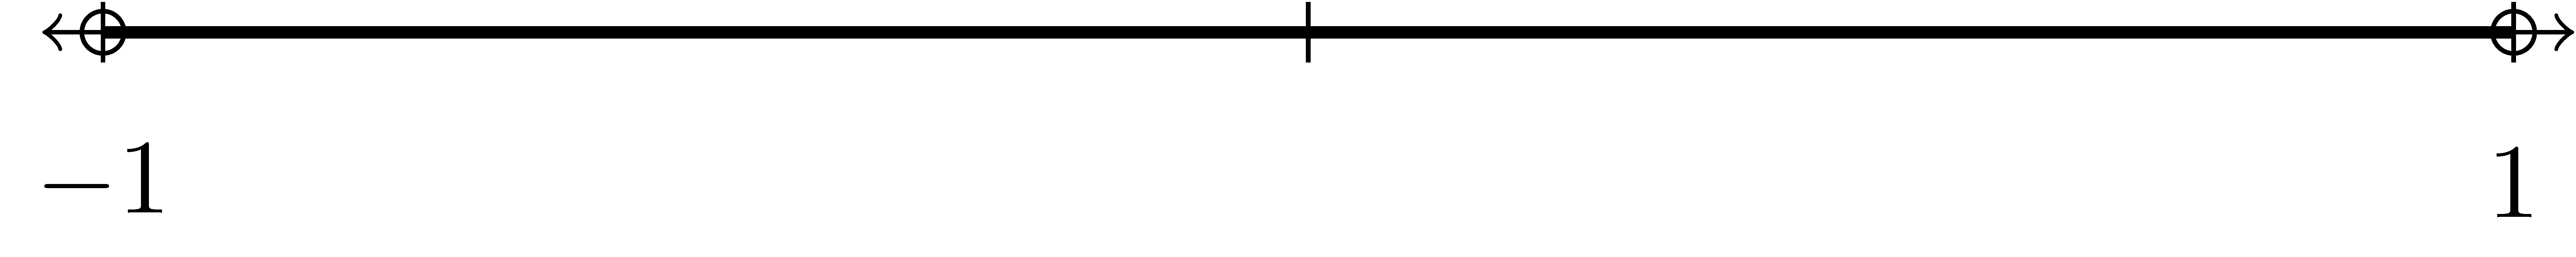
\includegraphics[width=0.35\linewidth]{tikz/Nested_s1} 

}

\end{figure}

\[S_2=(\frac{-1}{2}, \frac{1}{2})\]

\begin{figure}

{\centering 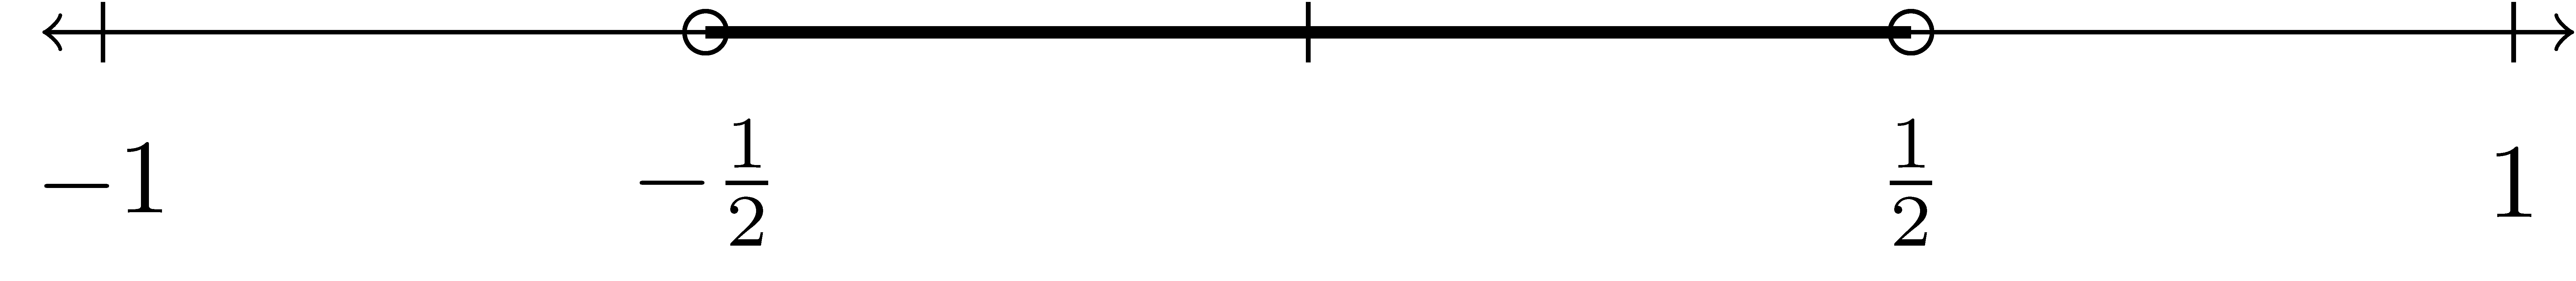
\includegraphics[width=0.35\linewidth]{tikz/Nested_s2} 

}

\end{figure}

\[S_3=(\frac{-1}{3}, \frac{1}{3})\]

\begin{figure}

{\centering 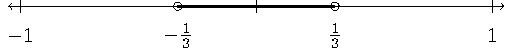
\includegraphics[width=0.35\linewidth]{tikz/Nested_s3} 

}

\end{figure}

Then we can see that for any \(i<j\), we have that \(S_i\cap S_j = S_j\) and \(S_i \cup S_j = S_i\).

We can also take the union and intersections over the entire collection of sets.
\[ \bigcup_{n\in \mathbb{N}} S_n = (-1,1) \quad \mbox{ and } \quad \bigcap_{n\in \mathbb{N}} S_n = \{0\}.\]

The above example is also an example of what is called a \textbf{nested} collection of sets.

\begin{definition}
\protect\hypertarget{def:unnamed-chunk-35}{}{\label{def:unnamed-chunk-35} } An indexed collection of sets, \(\left\{ A_i\right\}_{i\in I}\), with an order on \(I\) is called \textbf{nested} if either
\[ A_i \subseteq A_j \mbox{ whenever } i<j \quad \mbox{or} \quad A_i \supseteq A_j \mbox{ whenever } i<j.\]
When the indexing set is the natural numbers this is often denoted by \[A_0 \subseteq A_1 \subseteq A_2 \subseteq \cdots \quad \mbox{ or } \quad A_0 \supseteq A_1 \supseteq A_2 \supseteq \cdots.\]
\end{definition}

Using the ideas of indexing sets and families of sets, we can generalize De Morgan's Laws to a general collection of sets, the proofs of which are very similar to the proof in the case of two sets.

\begin{theorem}[Generalized De Morgan's Laws]
\protect\hypertarget{thm:unnamed-chunk-36}{}{\label{thm:unnamed-chunk-36} \iffalse (Generalized De Morgan's Laws) \fi{} }Let \(I\) be an indexing set and let \(\{A_i\}_{i\in I}\) be a collection of sets that are all subsets of the same universal set. Then
\[\left( \bigcup_{i\in I} A_i \right)^c = \bigcap_{i \in I} A_i^c \quad \mbox{and} \quad \left( \bigcap_{i\in I} A_i \right)^c = \bigcup_{i \in I} A_i^c\]
\end{theorem}

\hypertarget{exercises-5}{%
\subsection{Exercises}\label{exercises-5}}

\begin{enumerate}
\def\labelenumi{\arabic{enumi}.}
\item
  For each of the following collections of sets:

  \[\displaystyle{\mathcal{A} = \left\{ \left[ \frac{1}{n},n\right) \right\}_{n=2,3,4,\ldots }}\]

  \[\displaystyle{\mathcal{B} = \left\{ \left( n,\infty \right) \right\}_{n=0,1,2,3,4,5,\ldots} }\]

  \[\displaystyle{\mathcal{C} = \left\{ \left[ -n, n \right] \right\}_{n=0,1,2,3,4,5,\ldots }}\]

  \[\displaystyle{\mathcal{D} = \left\{ [x,x+1)\right\}_{x\in \mathbb{R}}}\]

  \[\displaystyle{\mathcal{E} = \left\{ \{z\in \mathbb{C}\middle \vert|z|=r\}\right\}_{r\in \mathbb{R}^+} }\]

  \[\displaystyle{\mathcal{F} = \left\{ \{n\in \mathbb{Z}\middle \vert n=3k+j \mbox{ for some } k\in \mathbb{Z}\}\right\}_{j=0,1,2}}\]

  \begin{enumerate}
  \def\labelenumii{\alph{enumii}.}
  \tightlist
  \item
    Determine if the sets are mutually disjoint
  \item
    Determine if the collection is nested
  \item
    Find the union of the collection
  \end{enumerate}
\end{enumerate}

\hypertarget{ch:equivalence}{%
\chapter{Equality, Order, and Equivalence}\label{ch:equivalence}}

The chapter title may look like just a list, but the notions of equality, order, and equivalence are a critically important trio of related but distinct ideas in mathematics. Together they help us define when two things are the ``same.'' Instruction in these ideas starts on almost the first day of school when students first learn how to count. Students continue study and expand these ideas in their study of mathematics: many of the theorems of mathematics labeled as ``Fundamental'' are statements of equivalence. These include the Fundamental Theorem of Arithmetic that every integer can be uniquely factored into primes, the Fundamental Theorem of Calculus describing the relationship between antiderivatives and infinite sums, and isomorphism theorems of abstract algebra and homeomorphisms of topology.

\hypertarget{partitions-and-equivalence-relations}{%
\section{Partitions and Equivalence Relations}\label{partitions-and-equivalence-relations}}

\begin{figure}

{\centering 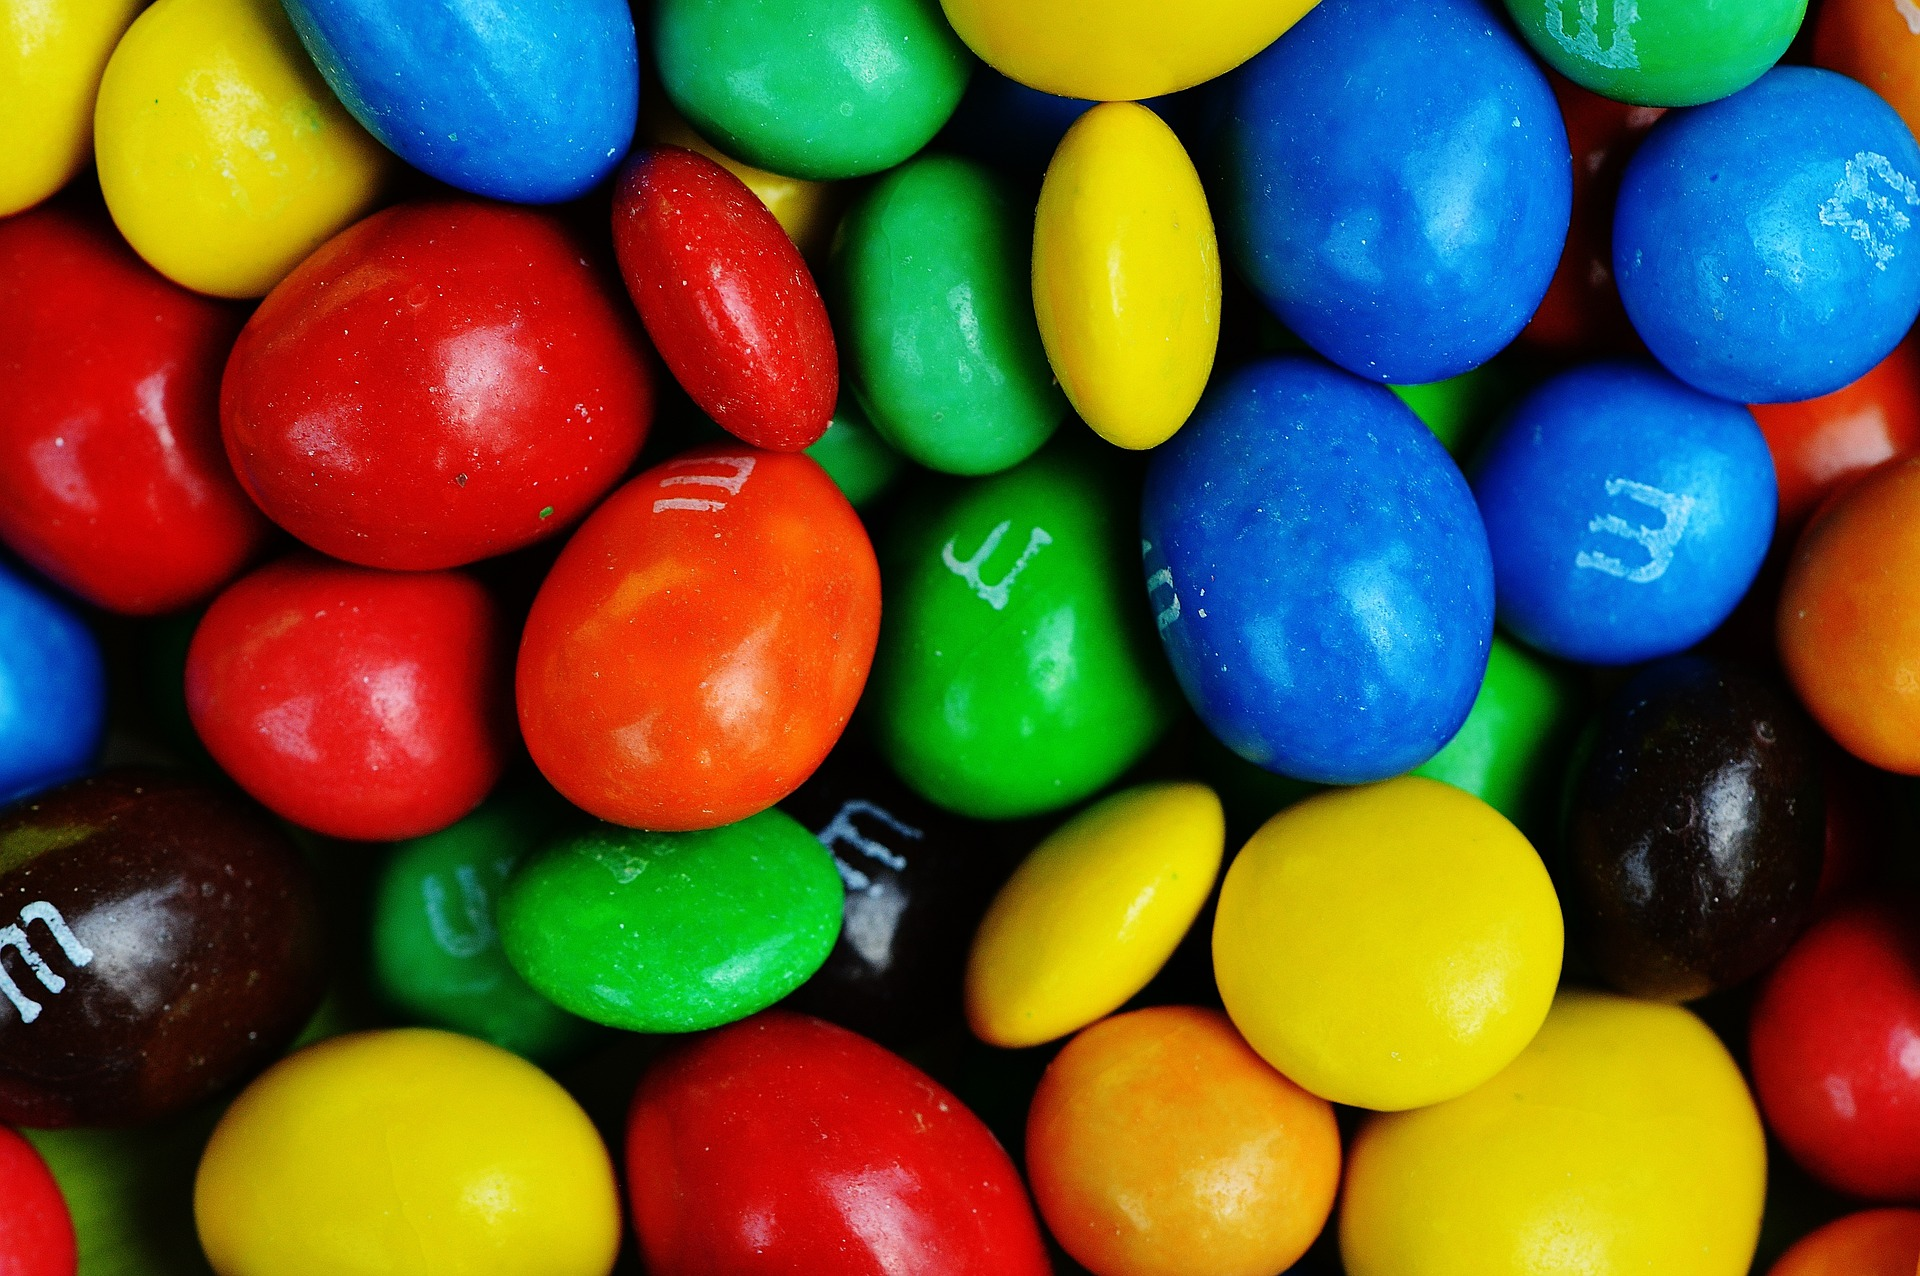
\includegraphics[width=0.5\linewidth]{images/m-and-m-1308543_1920} 

}

\caption{Sorting Candy}\label{fig:unnamed-chunk-37}
\end{figure}

As a way to better understand the world, humans tend to sort information into categories or orderings. For instance, when some people see a pile of various types of M\&M'sTM they have the urge to sort them in various ways. Some people sort the candies according to their color. Others may sort them according to their type (plain, peanut, etc.). This process of sorting is a type of ``partitioning'' the items into distinct categories. With this categorization we want to make sure that each candy is sorted into one, and only one, type. This type of sorting can be formalized with the following definition.

\hypertarget{partitions}{%
\subsection{Partitions}\label{partitions}}

\begin{definition}
\protect\hypertarget{def:unnamed-chunk-38}{}{\label{def:unnamed-chunk-38} } A \textbf{partition} of a set \(A\) is a finite or infinite collection of non-empty, mutually-disjoint subsets whose union is \(A\). \index{Partition}
\end{definition}

\begin{figure}

{\centering 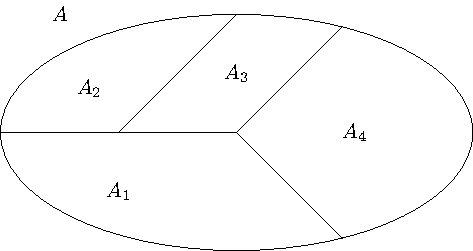
\includegraphics[width=0.5\linewidth]{tikz/Set_partition} 

}

\caption{Partition of Sets}\label{fig:unnamed-chunk-39}
\end{figure}

Thus, a partition of a set is a collection of subsets of the original set with several key properties. First, the subsets are non-empty, meaning that each subset in the partition contains at least one element. This allows us to restrict the partition to a collection of non-trivial subsets and means partitions have a type of uniqueness. The subsets in the partition are also mutually-disjoint which means that no element of the original set is in more than one of the subsets in the partition. Lastly, since the union of the subsets that form the partition is \(A\), we have that every element in \(A\) is in one of these subsets. Thus, each component of the definition of a partition is essential to defining a way to split a set into a set of categories that we find useful.

\begin{example}
\protect\hypertarget{exm:unnamed-chunk-40}{}{\label{exm:unnamed-chunk-40} }If we have a set
\[A=\left\{ a, 2, \alpha , \mbox{apple} , \mbox{box}, \beta, 1, 3, \gamma , \mbox{cow}, c, b \right\}\] there are some natural ways to partition the set. Here are three possible partitions.

\[
            A_1 = \{a,b,c\}, \:
            A_2 = \{1,2,3\},\: 
            A_3 = \{\alpha, \beta, \gamma\}, \: 
            A_4 = \{\mbox{apple} , \mbox{box}, \mbox{cow}\} 
\]
\[
            A_1 = \{\mbox{apple} , \mbox{box}, \mbox{cow}\}, \:
            A_2 = \{a,b,c,1,2,3,\alpha,\beta,\gamma\}
\]
\[
            A_1 = \{a,1,\alpha,\mbox{apple}\}, \: 
            A_2 = \{b,2,\beta,\mbox{box}\}, \: 
            A_3 = \{c,3,\gamma, \mbox{cow} \}
\]

There are many other ways to partition the set, but we do not have the space to write out all of the possible partitions of this set.
\end{example}

\begin{example}
\protect\hypertarget{exm:unnamed-chunk-41}{}{\label{exm:unnamed-chunk-41} } Early in the K-12 mathematics curriculum we ask students to determine which integers are even and which are odd. In this situation, the set \(A\) is the set of integers (\(\mathbb{Z}\)), while the subsets that form the partition are the subset of even numbers, (\(2\mathbb{Z}\)), and odd numbers, (\(2\mathbb{Z}+1\)).
\end{example}

\begin{example}
\protect\hypertarget{exm:unnamed-chunk-42}{}{\label{exm:unnamed-chunk-42} }If we let the set \(B\) be defined by the following list of elements,
\[B = \begin{Bmatrix} 
\mbox{ jar},  & \mbox{ jellybean} ,  & \mbox{ applesauce}, & \mbox{ ape}, & \mbox{ bear}, \\
\mbox{ ball}, & \mbox{ beanbag}, & \mbox{ bag}, & \mbox{ arm} , & \mbox{ skate} , \\
\mbox{ bike}, & \mbox{ rock}, & \mbox{ rowboat},   &  \mbox{ jigsaw}, & \mbox{ saw}
 \end{Bmatrix}\]
take some time to create various partitions of the set \(B\), verifying the various properties in the definition of a partition.
\end{example}

In this text, we denote the partition \(\mathcal{P}\) of a set \(A\) as the union of subsets of \(A\) over some indexing set, \(I\). For example, if the partition is formed using two subsets of \(A\), then the indexing set could be \(I=\{1,2\}\). The indexing set can also be infinite. For instance,
\[\mathcal{P} = \left\{ A_n  \right\}_{n\in \mathbb{Z}}, \: \mbox{ where } A_n=\left\{x\in \mathbb{R}\middle \vert n\leq x < n+1  \right\}\] is a partition of the real numbers with an infinite number of sets.

It is important to note that there are usually many ways to partition a set, but the definition of partition does not impose any constraints on the uniformity or order of the subsets, only that the way we choose our subsets meets the three conditions described previously.

With our previous discussion and examples in mind, we can translate our verbal definition of a partition into a symbolic one. In particular: if \(\mathcal{P}= \left\{ U_i\right\}_{i\in I}\) is a partition of a set \(A\), where \(I\) is some indexing set that is either finite or infinite, we have the following properties
\[U_i \bigcap U_j = \emptyset \quad \mbox{if } i\neq j, \quad \bigcup_{i\in I} U_i = A \mbox{, and} \quad U_i \neq \emptyset \mbox{ for all } i \in I.\]

\hypertarget{relations}{%
\subsection{Relations}\label{relations}}

Up until this point we have focused on building a framework for understanding the notion of partition. In order to understand the main topics of this chapter, we also need to develop the idea of a relation. While we give the general definition of a relation and a few examples, we will focus on those relations that arise from partitions in this section. We will explore other types of relations in later sections.

\begin{definition}
\protect\hypertarget{def:unnamed-chunk-43}{}{\label{def:unnamed-chunk-43} }Let \(A\) and \(B\) be sets. We define a relation \(R\) from \(A\) to \(B\) as a subset of \(A\times B\). We say that for elements \(a\in A\) and \(b\in B\) that \(a\) is related to \(b\), (\(aRb\)), if and only if \((a,b)\in R\). If the two sets are the same set, \(A\), then we say that \(R\) is a relation on \(A\).
\end{definition}

Here are some examples of relations in the K-12 curriculum.

\begin{itemize}
\item
  Let \(A\) and \(B\) be the set of integers. We could say that \[R=\{(a,b)\in A\times B \vert a<b\},\] which defines the `less than' relation of \(aRb \leftrightarrow a<b\).
\item
  Let \(A\) be the real numbers and \(B\) be the non-negative real numbers. We can let \[R=\{(x,y)\in A\times B \vert y=x^2\}.\] This is the graph of the function \(f(x)=x^2\).
\item
  Let \(A\) and \(B\) be the set of integers. We can define \[R= \{(m,n) \vert m-n=2k, \: \mbox{ for some integer } k\}.\] This relation is one where are the even numbers are related to each other and all of the odd numbers are related to each other.
\end{itemize}

\hypertarget{equivalence-relations-induced-by-partitions}{%
\subsection{Equivalence Relations Induced by Partitions}\label{equivalence-relations-induced-by-partitions}}

For the remainder of this section we will study a specific type of relation that is created by a partition, \(\mathcal{P}\), of a set, \(A\). If \(\mathcal{P}=\left\{U_i\right\}_{i\in I}\) is a partition of \(A\), we can write \(A\) as the union of a collection of non-empty, mutually disjoint subsets: \[U_i \cap U_j = \emptyset \mbox{ if } i\neq j, \: \mbox{ for each } i \in I, \: U_i\neq \emptyset, \: \mbox{ and } A=\bigcup_{i\in I} U_i.\]

Consider one of the individual subsets in the partition, say \(U_i\). Then the elements of \(U_i\), by virtue of the fact they are in the same subset, have a relationship to each other. This idea extends to the whole partition. That is, the partition induces a relation on \(A\) in the following way. For each \(a,b\in A\) we say that \(aRb\) if, and only if, there is a set \(U_i\) in the partition \(P\) such that both \(a\) and \(b\) are in \(U_i\).

The relations we create through a partition behave in ways that are of general interest in the study of mathematics.

If we choose a generic element \(a\) in \(A\), the property that \(\bigcup_{i\in I} U_i = A\) tells us that there exists \(i\in I\) such that \(a \in U_i\). So for every element \(a\in A\), we have that \(aRa\). We will call this property of the relation the \textbf{reflexive property}.

For the second property, if we have \(a,b\in A\) such that \(aRb\), then there must be a \(U_i\in P\) with \(a,b\in U_i\). This also means that \(bRa\). When you have the property that \(aRb\) implies that \(bRa\), we say that the relation has the \textbf{symmetric property}.

The third property of relations that we define derives from the property of partitions that
\[U_i \bigcap U_j = \emptyset \Leftrightarrow i\neq j.\] If \(a,b,c\in A\) such that \(aRb\) and \(bRc\), then we have that there are sets \(U_i\) and \(U_j\) in the partition such that \(a\) and \(b\) are both in \(U_i\) and \(b\) and \(c\) are both in \(U_j\). Since \(b\) is in both \(U_i\) and \(U_j\), \(U_i \cap U_j \neq \emptyset\) and so \(i=j\). This would then imply that \(aRc\). This property that the combination of \(aRb\) and \(bRc\) implies that \(aRc\) is called the \textbf{transitive property} of relations.

Not all relations have these three properties of reflexive, symmetric, and transitive. Those relations that have all three properties are called \textbf{equivalence relations}.

We have therefore proven that a partition of a set induces an equivalence relation on that set.

\hypertarget{partitions-induced-by-equivalence-relations}{%
\subsection{Partitions Induced by Equivalence Relations}\label{partitions-induced-by-equivalence-relations}}

The concept of equivalence relation is one that transcends much of mathematics and we often consider things as being the ``same'' with respect to some property if there is an equivalence relation under which they are related. One location that this appears in the elementary school curriculum is in regards to rational numbers. We think of \(\frac{1}{2}\) and \(\frac{2}{4}\) as being the same rational number, but written in a different way. Along these lines we say that two rational expressions \(\frac{a}{b}\) and \(\frac{c}{d}\) are equivalent if and only if \(ad=bc\). This creates and equivalence relation between these rational expressions that are used to create the rational numbers.

Similarly, if a relation, \(R\), on a set, \(A\), is an equivalence relation, then one can generate an induced partition, \(\mathcal{P}\), as follows. For each \(a\in A\) we define the set \[[a]_R := \left\{ b\in A \middle \vert aRb\right\}.\] We call this set, \([a]_R\), the equivalency class of \(a\) under the relation \(R\).

Since \(R\) is an equivalence relation, it is reflexive and so \(a \in [a]_R\) causing \([a]_R \neq \emptyset\). Since \(a\in [a]_R\), we have that \[\bigcup_{a\in A} [a]_R = A.\] Thus to show that \(\mathcal{P} = \left\{ [a]_R \middle \vert a \in A\right\}\) is a partition of \(A\), we need to show that for \(a,b\in A\) that \([a]_R=[b]_R\) or \([a]_R\bigcap [b]_R = \emptyset\).

If \([a]_R \bigcap [b]_R \neq \emptyset\), then we need to prove that two sets to be equal.

Let us assume that there exists a \(c\in [a]_R \bigcap [b]_R\).

Let \(d\in [a]_R\). So \(a R d\). \(c\) is also in \([a]_R\) and so \(aRc\). Since \(R\) is symmetric and \(aRd\), \(dRa\). We now have that \(dR c\) using transitive property. \(c\) is also in \([b]_R\) and so \(bRc\). Using the symmetric property, we have \(cR b\). Combining this with \(dRc\) and using the transitive property we have \(dR b\). Using the symmetric property we have \(bR d\). So \(d\in [b]_R\). Therefore, \([a]_R \subseteq [b]_R\).

Using very similar arguments we can prove that \([b]_R \subseteq [a]_R\).

So if the intersection is nonempty, the two sets are the same set.

We have thus proven the following theorem showing the connection between equivalence classes and partitions.

\begin{theorem}
\protect\hypertarget{thm:unnamed-chunk-44}{}{\label{thm:unnamed-chunk-44} }If \(R\) is an equivalence relation on a set \(A\), then \[P = \left\{ [a]_R \middle \vert a \in A\right\}\] is a partition of \(A\).

Similarly, if \(P= \left\{ U_i \middle \vert i \in I\right\}\) is a partition on a set \(A\), then the relation \(R\) defined by
\[aRb \Leftrightarrow \mbox{ there exists } i \in I \mbox{ such that } a,b \in U_i\] is an equivalence relation.
\end{theorem}

\hypertarget{exercises-6}{%
\subsection{Exercises}\label{exercises-6}}

\begin{enumerate}
\def\labelenumi{\arabic{enumi}.}
\item
  Define a relation \(\sim\) on \(\mathbb{R}\times (\mathbb{R}-\{0\})\) by
  \[(x,y) \sim (z,w) \Leftrightarrow xw=yz.\]

  \begin{enumerate}
  \def\labelenumii{\alph{enumii}.}
  \tightlist
  \item
    Show that this relation is an equivalence relation.
  \item
    Give a description of the partition of \(\mathbb{R}\times (\mathbb{R}-\{0\})\) induced by this equivalence relation.
  \item
    Why do we not allow \(0\) in the second part of the ordered pairs?
  \end{enumerate}
\item
  Determine which of the following collections of sets form a partition of \(\mathbb{R}\times \mathbb{R}\). For those that do form a partition, define the equivalence relation.

  \begin{enumerate}
  \def\labelenumii{\alph{enumii}.}
  \tightlist
  \item
    For \(c\in \mathbb{R}\), let \(h_c= \{ (x,y)\in \mathbb{R}^2 \vert y=c\}\), and let \(\mathcal{C} = \{h_c\}_{c\in \mathbb{R}}\).
  \item
    For \(m\in \mathbb{R}\), let \(s_m=\{ (x,y)\in \mathbb{R}^2 \vert y=mx\}\), and let \(\mathcal{D}= \{s_m\}_{m\in \mathbb{R}}\).
  \item
    For \(r\in [0,\infty)\), let \(C_r=\{ (x,y) \in \mathbb{R}^2 \vert x^2+y^2=r^2\}\), and let \(\mathcal{E}=\{C_r\}_{r\in [0,\infty)}\).
  \end{enumerate}
\item
  (For students who have knowledge of linear algebra) Let \(M_{2,2}\) be the set of \(2 \times 2\) matrices with real coefficients. For each of the following, prove that it is an equivalence relation, or show that one of the properties of equivalence relations does not hold.

  \begin{enumerate}
  \def\labelenumii{\alph{enumii}.}
  \tightlist
  \item
    For matrices \(A\) and \(B\) in \(M_{2,2}\), let \(A \sim B\) if and only if \(\mathrm{det}(A)=\mathrm{det}(B)\).
  \item
    For matrices \(A\) and \(B\) in \(M_{2,2}\), let \(A \sim B\) if and only if \(\mathrm{tr}(A)=\mathrm{tr}(B)\).
  \item
    For matrices \(A\) and \(B\) in \(M_{2,2}\), let \(A \sim B\) if and only if the eigenvalues of \(A\) are the same as the eigenvalues of \(B\).
  \end{enumerate}
\end{enumerate}

\hypertarget{ordered-sets-and-relations}{%
\section{Ordered Sets and Relations}\label{ordered-sets-and-relations}}

In the previous section we defined a relation \(R\) from \(A\) to \(B\) as a subset of \(A\times B\), and that \(a\) is related to \(b\), (\(aRb\)), if and only if \((a,b)\in R\). If the two sets are the same set, \(A\), then we say that \(R\) is a relation on \(A\).

We also defined the following three properties of a relation, \(R\), on a set \(A\):

\begin{itemize}
\tightlist
\item
  \textbf{Reflexive.} The relation \(R\) is reflexive if \(aRa\) for all \(a\in A\).
\item
  \textbf{Symmetric.} The relation \(R\) is symmetric if \(aRb\) implies that \(bRa\) for all \(a,b\in A\).
\item
  \textbf{Transitive.} The relation \(R\) is transitive if \(aRb\) and \(bRc\) imply that \(aRc\) for \(a,b,c\in A\).
\end{itemize}

A relation is an equivalence relation if it satisfies all three of these properties. Another type of relation is one that creates an order, or ranking, of the set. A common mathematical topic in this regards are the concepts of ``less than'' and ``less than or equal to''.

We will first explore the relation of ``less than''. Since a number cannot be less than itself we see that the relation is not reflexive. We also know that \(a<b\) and \(b<a\) cannot both be true and so the relation is not symmetric. However, if \(a<b\) and \(b<c\) we do have that \(a<c\). So this relation of ``less than'' is transitive. Thus the familiar relation of ``less than'' is one which is transitive but not reflexive or symmetric.

When we expand the relation to that of ``less than or equal to'', we add that \(a\leq a\), resulting in the relation being reflexive. So this is a common relation that is reflexive and transitive, but not symmetric. For example, \(1\leq 2\), but \(2\) is not less than or equal to \(1\).

\begin{definition}
\protect\hypertarget{def:unnamed-chunk-45}{}{\label{def:unnamed-chunk-45} }We define an \textbf{order} on a set, \(A\), to be a relation, denoted by \(<\), with the following properties.

\begin{enumerate}
\def\labelenumi{\arabic{enumi}.}
\tightlist
\item
  If \(x\) and \(y\) are two elements of \(A\), then one, and only one, of the statements \[x<y, \quad x=y, \quad, y<x\] is true.
\item
  If \(x,y,z \in A\), and if \(x<y\) and \(y<z\), then \(x<z\).
\end{enumerate}

If a set has an order defined on the set, then we say that it is an \textbf{ordered set}.
\end{definition}

Such an order forms a relation that is transitive, but not symmetric or reflexive. As a convenient notation, we will write \(x\leq y\) as the negation of \(y<x\). We then see that it is equivalent to the statement that (\(x<y\) or \(x=y\)).

\begin{definition}[Well-Ordering Property]
\protect\hypertarget{def:well-ordering}{}{\label{def:well-ordering} \iffalse (Well-Ordering Property) \fi{} }A set, \(A\), together with an order, \(<\), satisfies the well-ordering property if every non-empty subset of \(A\) has a least element. Equivalently, if \(S\subseteq A\) with \(S\neq \emptyset\), then there exists an element \(s_0\in S\) such that \(s_0 \leq s\) for all \(s\in S\).
\end{definition}

We will see in Chapter \ref{ch:number} that the natural numbers, \(\{0,1,2,3,\ldots\}\), satisfy the well-ordering property, but the real numbers do not. For instance, \(\{x\in \mathbb{R}\vert x>1\}\) does not have a least element. This means that in some way, a set needs to be discrete in order to satisfy a well-ordering property.

For sets that are not discrete, we would like to have a similar property.

\begin{definition}
\protect\hypertarget{def:unnamed-chunk-46}{}{\label{def:unnamed-chunk-46} }Let \(A\) be an ordered set and let \(S\subseteq A\). If there exists an \(\alpha \in A\) such that \(x\leq \alpha\) for all \(x\in S\), then we say that \(S\) is \textbf{bounded above} and that such an \(\alpha\) is an \textbf{upper bound} of \(S\).
\end{definition}

We can similarly define \textbf{bounded below} and \textbf{lower bound} using opposite inequalities.

\begin{definition}[Least-Upper-Bound Property]
\protect\hypertarget{def:unnamed-chunk-47}{}{\label{def:unnamed-chunk-47} \iffalse (Least-Upper-Bound Property) \fi{} }An ordered set \(A\) is said to have the \textbf{least-upper-bound property} if for every non-empty subset \(S\subseteq A\) that is bounded above, there exists an element \(s_0\in S\) such that \(s_0\) is an upper bound of \(S\) and if \(\alpha\) is an upper bound of \(S\), then \(s_0\leq \alpha\). Such an \(s_0\) is called the \textbf{least-upper-bound} of \(S\).
\end{definition}

We will see in Chapter \ref{ch:number} that the real numbers satisfy the least-upper-bound property, while the rational numbers do not.

\hypertarget{exercises-7}{%
\subsection{Exercises}\label{exercises-7}}

\begin{enumerate}
\def\labelenumi{\arabic{enumi}.}
\tightlist
\item
  For each of the following relations, determine if the relation is reflexive, symmetric, and/or transitive.

  \begin{enumerate}
  \def\labelenumii{\alph{enumii}.}
  \tightlist
  \item
    Let \(S\) be a relation defined on \(\mathbb{R}\) by \[xSy \Leftrightarrow x^2=y^2.\]
  \item
    Let \(T\) be a relation defined on \(\mathbb{R}\) by \[xTy \Leftrightarrow x<y^2.\]
  \item
    Let \(U\) be a relation defined on \(\mathbb{Z}\) by \[mTn \Leftrightarrow mn>0.\]
  \item
    Let \(V\) be a relation defined on \(\mathbb{R}^2\) by \[ (x,y)V(w,z) \Leftrightarrow x^2+y^2 \leq w^2+z^2.\]
  \end{enumerate}
\item
  Let \(S=\{a,b\}\). List out all of the possible relations on \(S\) and determine which relations are reflexive, symmetric, and/or transitive.
\end{enumerate}

\hypertarget{equality-and-equivalence-in-the-k-12-curriculum}{%
\section{Equality and Equivalence in the K-12 Curriculum}\label{equality-and-equivalence-in-the-k-12-curriculum}}

We can see from the discussion in the previous two sections that the concept of two things being equivalent mathematically is a very difficult and abstract concept. It is no surprise then that students of all grade levels have many different conceptions and misconceptions revolving around this concept of equality and equivalence.

Since all of the number systems that arise in the elementary and early secondary curriculum have an inherent order described by the \(\leq\) and \(<\) symbols, the concept of equality is often described in terms of a balanced scale. Another conception around the equal sign is that two sets of objects have the same number of items, determined by counting the number of objects. This is likely since the concept of equality arises in the first grade where students are only working with whole numbers.

\begin{figure}

{\centering 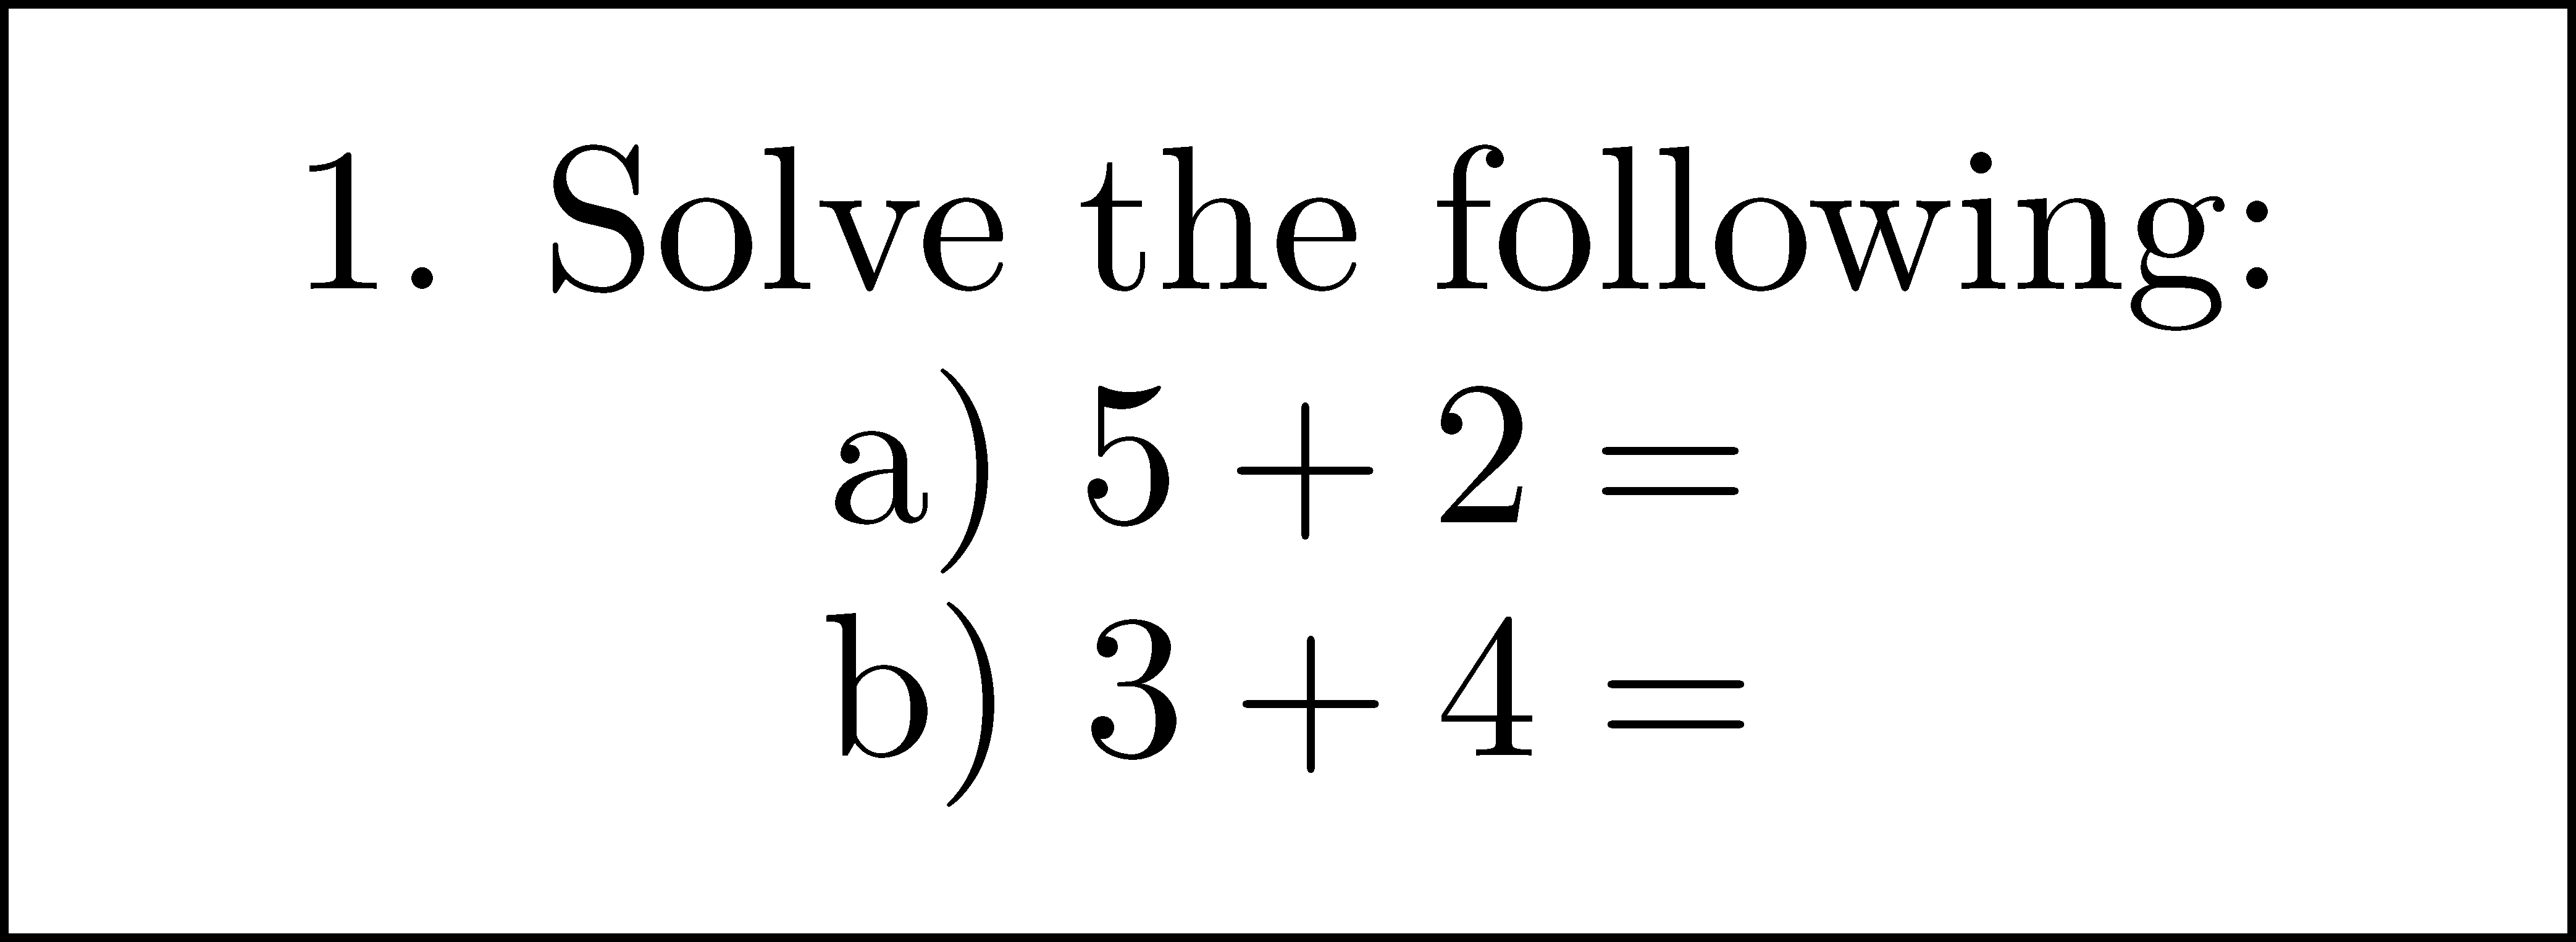
\includegraphics[width=0.35\linewidth]{tikz/sample_addition_problem} 

}

\caption{Sample problems}\label{fig:equality-operation}
\end{figure}

One of the common misconceptions surrounding the equal sign is that the symbol implies an action of doing some type of computation. For instance, students usually see the equal sign in the context of the type of problems seen in Figure @ref\{fig:equality-operation\}.

These type of problems promote an operational understanding of the equal sign, rather than a relational or substitutional understanding that is essential for later work \citep[pp.~145-150]{Cognition}. Because secondary mathematics students maintain many misconceptions about the concept of equality and the meaning of the equal sign, we will take some time to reflect on some key content standards from first grade that have a very strong influence on student success of learning mathematics in the middle school.

\begin{quote}
\hypertarget{related-content-standards-3}{%
\subsubsection*{Related Content Standards}\label{related-content-standards-3}}
\addcontentsline{toc}{subsubsection}{Related Content Standards}

\begin{itemize}
\tightlist
\item
  (1.OA.7) Understand the meaning of the equal sign, and determine if equations involving addition and subtraction are true or false. For example, which of the following equations are true and which are false? \(6 = 6\), \(7 = 8 - 1\), \(5 + 2 = 2 + 5\), \(4 + 1 = 5 + 2\).
\item
  (1.OA.8) Determine the unknown whole number in an addition or subtraction equation relating three whole numbers. For example, determine the unknown number that makes the equation true in each of the equations \(8 + ? = 11\), \(5 = ? - 3\), \(6 + 6 = ?\).
\end{itemize}
\end{quote}

\begin{figure}

{\centering \includegraphics[width=0.4\linewidth]{images/balance-scales} 

}

\caption{Pan balances}\label{fig:pan-balance}
\end{figure}

We should notice that in standard (1.OA.D.8) that the unknown should not always be at the end of a string of mathematical symbols and is based on educational research that compares students from different cultures and their understanding of the equal sign \citep[pp.~148-150]{Cognition}. Instead it should be at many different locations in order to make sure that students do not internalize the misconception that the equal sign means to compute. They should instead develop the concept of the equal sign representing two things that have the same value in some way. It is this understanding of two things looking different but representing the same underlying value that causes the equal sign to represent an equivalence.

Another method that may possibly contribute to a more relational understanding of the equal sign is the introduction of the equal sign alongside the greater than (\(>\)) and less than (\(<\)) symbols to emphasize the role of the equal sign in the comparison of the size of numbers. This comparison concept can be further reinforced with a pan balance (See Figure \ref{fig:pan-balance}).

This concept of a pan-balance can give students a concrete idea to attach to the meaning of the equal and inequality signs. However, like all good analogies, the pan balance is challenging to use with negative numbers and breaks down if you are comparing numbers in an unordered number system such as the complex numbers.

\hypertarget{exercises-8}{%
\subsection{Exercises}\label{exercises-8}}

A student is given the following task.

\begin{quote}
\begin{itemize}
\tightlist
\item
  Sophia goes to the store with \(\$5.00\) and buys two packs of gum for \(\$1.20\). She then gives \(\$2.00\) to her friend to buy a drink. How much money does she have left?
\end{itemize}
\end{quote}

\begin{enumerate}
\def\labelenumi{\arabic{enumi}.}
\item
  The student then writes the following on their paper.
  \[5.00-1.20=3.80-2.00=1.80, \mbox{ so Sophia has } \$1.80 \mbox{ left.}\]

  \begin{enumerate}
  \def\labelenumii{\alph{enumii}.}
  \item
    What ideas from this section regarding the equal sign and equivalence would you use to provide feedback to this student?
  \item
    What are other points of feedback that you would provide to this student?
  \end{enumerate}
\item
  If a student asks you what the equal sign means in the context of \(\frac{1}{2}=\frac{2}{4}\) since those symbols are not the same.
\item
  What are the meanings of the equal signs in the task?
  \textgreater Evaluate the function \(f(x)=3x-4\) for \(x=2\).
\end{enumerate}

\hypertarget{expressions-equations-and-inequalities}{%
\section{Expressions, Equations, and Inequalities}\label{expressions-equations-and-inequalities}}

A \textbf{numerical expression} is a meaningful string of numbers, operation symbols, and/or grouping symbols. In early elementary grades, examples of numerical expressions include \[2+6+4, \quad 13-3+2, \quad \mbox{ or } \quad (4+6)+3.\] In upper elementary grades, students are expected to incorporate rational numbers and the operations of multiplication, division, and exponents in order to be comfortable working with such expressions as
\[3 \times (10+4), \quad \frac{2}{3} \times (12+8), \quad \mbox{ or } \quad  2^3 + \frac{3+2}{7}.\]

In the transition from elementary school to secondary schools, students learn to add \textbf{variables}, symbols or letters that stand for any number within a specified range of numbers, to these expressions and thus work with \textbf{algebraic expressions} such as
\[100-10\cdot (P-15)^3,  \quad 3xy + 5(x-4)^2-7y^2, \quad 6\cdot (4x+3y), \quad \mbox{ or }\quad  \frac{3x+2}{2x-4}.\]

\begin{quote}
\hypertarget{related-content-standards-4}{%
\subsubsection*{Related Content Standards}\label{related-content-standards-4}}
\addcontentsline{toc}{subsubsection}{Related Content Standards}

\begin{itemize}
\tightlist
\item
  (6.EE.2) Write, read, and evaluate expressions in which letters stand for numbers.
\end{itemize}

\begin{enumerate}
\def\labelenumi{\alph{enumi}.}
\tightlist
\item
  Write expressions that record operations with numbers and with letters standing for numbers.
\item
  Identify parts of an expression using mathematical terms (sum, term, product, factor, quotient, coefficient); view one or more parts of an expression as a single entity.
\item
  Evaluate expressions at specific values of their variables. Include expressions that arise from formulas used in real-world problems. Perform arithmetic operations, including those involving whole-number exponents, in the conventional order when there are no parentheses to specify a particular order (Order of Operations).
\end{enumerate}
\end{quote}

In more advanced courses in secondary school mathematics, algebraic expressions can also include functions giving rise to expressions such as
\[f(x-h)+k, \quad \sin(3x)-2, \quad \mbox{ or } \quad  \ln(x+3).\]

The equivalence of numerical expressions is a key concept in the early elementary grades where students learn to compose and decompose numbers in different ways as they add and subtract numbers using different algorithms. In sixth grade, students are asked to determine the equivalence of two mathematical expressions. This definition that two algebraic expressions are equivalent if they generate the same number regardless of which number is substituted for the variable is one of the first places where students are pushed to move to the abstract realm of equivalence relations. We can verify that this definition of equivalent expressions is an equivalence relation using the fact that equality on the real numbers is an equivalence relation.

\begin{quote}
\hypertarget{related-content-standards-5}{%
\subsubsection*{Related Content Standards}\label{related-content-standards-5}}
\addcontentsline{toc}{subsubsection}{Related Content Standards}

\begin{itemize}
\tightlist
\item
  (6.EE.3) Apply the properties of operations to generate equivalent expressions. \%\{\em For example, apply the distributive property to the expression $3 (2 + x)$ to produce the equivalent expression $6 + 3x$; apply the distributive property to the expression $24x + 18y$ to produce the equivalent expression $6 (4x + 3y)$; apply properties of operations to $y + y + y$ to produce the equivalent expression $3y$.\}
\item
  (6.EE.4) Identify when two expressions are equivalent (i.e., when the two expressions name the same number regardless of which value is substituted into them).
\item
  (6.EE.5) Understand solving an equation or inequality as a process of answering a question: which values from a specified set, if any, make the equation or inequality true? Use substitution to determine whether a given number in a specified set makes an equation or inequality true.
\end{itemize}
\end{quote}

While substituting in values to determine if two expressions are equivalent is the definition of the equivalence, it is almost always impossible to substitute in all possible values for a variable, as there are infinitely many possibilities in most situations. Instead, we determine the equivalency of two expressions by applying various properties of the operations. For example, the distributive property shows us that \(3(x+y)\) is equivalent to \(3x+3y\). However, students have to be careful to consider the set of possible numbers for an expression when determining the equivalence of \(\sqrt{x^2}\) and \(x\), or \(\frac{3x^2}{x}\) and \(3x\).

An \textbf{equation} is a statement that a number or expression is equivalent to a different number or expression. An equation that is true for all values of the variable is called an \textbf{identity}. The associative, commutative, and distributive properties of the number systems
\begin{align*}
    a+(b+c) &= (a+b)+c \\
    a+b &= b+a \\
    a \times (b+c) &= (a\times b)+(a\times c)
\end{align*}
are all common identities. Some other common identities in this regard are the trigonometric identity
\begin{align*}
    \cos^2(\theta) + \sin^2(\theta) &= 1  \\
    \sin(\alpha \pm \beta) &= \sin(\alpha)\cos(\beta)\pm \cos(\alpha)\sin(\beta) \\
    \cos(2\theta) &= \cos^2(\theta)-\sin^2(\theta)
\end{align*}
that are used to simplify trigonometric expressions.

An equation that describes how multiple quantities vary together is usually called a \textbf{formula}. These can include the area formula for rectangles defined by \(\mbox{Area}=\mbox{width} \times \mbox{height}\) or Boyle's law where pressure (\(P\)) is inversely proportional to volume (\(V\)), i.e.~\(PV =k\) for some constant \(k\).

While the identity equations hold true irrespective of the values of the variables, it is often the case that equations hold for only some of the possible values for the variables, or possibly even none. We can then \textbf{solve} such equations by determining which values, called \textbf{solutions to the equation}, for the variables cause the equation to be a true statement.

Similar to equations, \textbf{inequalities} are statements that a number or expression is related to a different number or expression in a certain order relation. Some of these inequalities are identities or formulas, such as \(x\leq |x|, x\in\mathbb{R}\), while some have a solution set, such as \(x^2+y^2<1\).

\begin{definition}
\protect\hypertarget{def:unnamed-chunk-48}{}{\label{def:unnamed-chunk-48} } Two equations (inequalities) are equivalent if they are true statements for the same values of the variables.
\end{definition}

In the process of finding solutions to equations or inequalities, it is almost always helpful to rewrite an equation or inequality as an equivalent equation or inequality. For instance in an effort to find the solutions to \[\frac{x^2-10x+21}{3x-12} = \frac{x-5}{x-4}\]
we want to find an expression that is equivalent to the left side of the equation. Such an expression could be \[\frac{(x-3)(x-7)}{3(x-4)},\] with the equivalency of the expressions verified using the distributive property. Since these two expressions are equivalent, they have the same values for every value of the variable. This means that the original equation is a true statement if, and only if, \[\frac{(x-3)(x-7)}{3(x-4)}=\frac{x-5}{x-4}\] is a true statement. We also know that if two numbers are the same, then \(3\) times each of the numbers are also the same. So the original statement is true if, and only if, the equivalent equation
\[\frac{(x-3)(x-7)}{x-4}=\frac{3(x-5)}{x-4}\] is true. If \(x=4\), then the statement would have no meaning, as division by zero has no meaning. This means that we can eliminate \(4\) from the set of possible solutions. With \(x\neq 4\) we can multiply both sides of the equation by \((x-4)\) to generate the equivalent equation, \[(x-3)(x-7)=3(x-5).\] We can use the distributive property again to create an equivalent equation of \[x^2-10x+21=3x-15.\] Since we can also add the same expression, \(-3x+15\), to both sides of the equation and create an equivalent equation, we see that the original equation is equivalent to \[x^2-13x+36=0\] as long as \(x\neq 4\). Using the distributive property, we see that this equation is equivalent to \[(x-4)(x-9)=0.\] So the original equation is a true statement if, and only if, \((x-4)(x-9)=0\) is a true statement and \(x\neq 4\). This only occurs when the variable, \(x\), is equal to \(9\).

Through this process we can see how equivalence of equations is essential in the process of finding solutions to equations. This means that as students make the transition from elementary to secondary, it is important for teachers to be understanding of the challenge of thinking about equivalent expressions and to be explicit about this relationship.

\hypertarget{exercises-9}{%
\subsection{Exercises}\label{exercises-9}}

\begin{enumerate}
\def\labelenumi{\arabic{enumi}.}
\tightlist
\item
  Most of this project will be in the context of algebraic reasoning and these questions should be answered with the expectations of your target student population.

  \begin{enumerate}
  \def\labelenumii{\alph{enumii}.}
  \tightlist
  \item
    What is the difference between an expression and equation?
  \item
    Why can we not solve an expression?
  \item
    What does it mean to ``solve an equation''?
  \item
    What makes two expressions equivalent to each other?
  \item
    What is the difference between how the equality sign is used when solving an equation versus when working with expressions?
  \end{enumerate}
\item
  Prove that the definition of equivalent equations forms an equivalency relation.
\end{enumerate}

\hypertarget{ch:number}{%
\chapter{Number Systems}\label{ch:number}}

K-12 mathematics is rich in the study of number systems, with particular focus on the Natural Numbers, Integers, Rational Numbers, Real Numbers, and Complex Numbers. In this chapter we use the properties of set theory and equivalence classes discussed in Chapters \ref{ch:sets} and \ref{ch:equivalence} to construct these numbers systems. We follow this discussion with a study of some of the properties of number systems, connecting them to the K-12 curriculum. Lastly, we examine different representations of these number systems helpful for developing numerical fluency and conceptual understanding of the numerical operations.

This process of constructing the number systems is very abstract and challenging for those who have not previously studied these constructions. The process is included because it helps teachers to better understand the abstract nature of the number systems and some of the challenges of their students. While working with many of these number systems has become second nature for math teachers, the initial learning by students is much harder than expected for new teachers and so a deeper knowledge of the properties of the number system helps in this teaching situation.

\[\mathbb{N} \subseteq \mathbb{Z} \subseteq \mathbb{Q} \subseteq \mathbb{R} \subseteq \mathbb{C}\]
As we are working with the various number systems, we will use varying notation for our operations. With all of the constructions, subtraction and division are not defined. We instead define the additive inverse and multiplicative inverse and so we can think of subtraction \(a-b\) as \(a+(-b)\) and division \(a\div b\) as \(a \times \frac{1}{b}\). We will also use various symbols to represent multiplication so that \(a\times b\), \(a\cdot b\), and \(ab\) all represent the same thing.

\hypertarget{sec:Integers}{%
\section{Natural Numbers and Integers}\label{sec:Integers}}

As part of the effort to axiomatize mathematics in the late 19\textsuperscript{th} and early 20\textsuperscript{th} centuries, individuals such as Richard Dedekind (1831-1916), Georg Cantor (1845-1918), Giuseppe Peano (1858-1932), Alfred Whitehead (1861-1947), David Hilbert (1862-1943), Ernst Zermelo (1871-1953), Bertrand Russell (1872-1970), and Abraham Fraenkel (1891-1965) followed a program to start with the most basic of assumptions and build a solid foundation for the field of mathematics. One of the greatest works in this program is the \emph{Principia Mathematica} by Whitehead and Russell \citetext{\citeyear{Principia1}; \citeyear{Principia2}; \citeyear{Principia3}} that built such a foundation on logic and set theory that it took until page 86 of the second volume to prove that \(1+1=2\). While we will not go to the full extent of abstraction, we will build up the natural numbers and the integers from the axioms of Zermelo-Fraenkel set theory, together with the axiom of choice (ZFC axioms).

\hypertarget{natural-numbers}{%
\subsection{Natural Numbers}\label{natural-numbers}}

We will study the concepts of counting and related ideas of the natural numbers in Chapter \ref{ch:function}, but initially we will use John von Neumann's \citeyearpar{vonNeumann23} definition for the natural numbers which are defined inductively by defining the symbols
\[0:=\emptyset, \quad 1:=\{\emptyset\}, \quad 2:=\{\emptyset, \{\emptyset\}\},\] and so on. So for any natural number \(n\), the next natural number is defined inductively as \[n+1:=S(n) := n\cup \{n\},\] where you think of \(S(n)\) as the successor of \(n\).

This definition of the natural numbers is highly dependent upon the axiom of infinity from the ZFC axioms. In the formal language of the ZFC axioms, the axiom of infinity is stated as
\[\exists I ( \emptyset\in I \wedge \forall x\in I((x\cup \{x\})\in I).\] Or equivalently, there is a set \(I\) that contains the empty set as an element and that if \(x\in I\), then \(x\cup \{x\}\) is also in \(I\). The set \(I\) is a larger set than \(\mathbb{N}\), but allows for the existence of the natural numbers.

With our definition of the natural numbers, we also have that \(S(n)\neq n\), \[S(n)=S(m) \Leftrightarrow n=m,\] and we can create an order on the set of symbols \(\mathbb{N} = \{0, 1, 2, 3, \ldots \}\) by defining that
\[n \leq m \Longleftrightarrow n \subseteq m.\] One can prove that this set of symbols satisfies the well-ordering property (@ref(def:well\_ordering)) using the ZFC axioms, which enables us to prove the principle of mathematical induction creating the mathematical machinery necessary for the study of the natural numbers.

\begin{theorem}[Principle of Mathematical Induction]
\protect\hypertarget{thm:unnamed-chunk-49}{}{\label{thm:unnamed-chunk-49} \iffalse (Principle of Mathematical Induction) \fi{} }Suppose that \(S\) is a subset of \(\mathbb{N}\) such that \(0\in S\), and for all \(n\in \mathbb{N}\), \(n\in S\) implies that \(S(n) \in S\).

Then \(S\) must be the set of natural numbers.
\end{theorem}

We will leave the detailed proof for a text on symbolic logic. However, the application of this theorem is that if we have a mathematical statement that varies along the natural numbers, \(P(n)\). If the statement \(P(0)\) is true, and if \(P(k)\) being true implies that \(P(k+1)\) is true, then \(P(n)\) must be true for all natural numbers.

We inductively define the operation of addition on these symbols so that for any integer \(a\),
\begin{align*}
    a+0 &:=a, \\
    a+1 := a+S(0) &= S(a+0), \\
    a+2:=a+S(1) &= S(a+1), \\
    \vdots \\
    a+S(b) &:= S(a+b)
\end{align*}
We similarly define multiplication inductively by
\[a\times 0 := 0, \quad a\times 1 := (a \times 0)+a = a, \quad \mbox{ and } \quad a\times S(b) := (a\times b)+a.\]
With these operations we have the following properties of the natural numbers.

\begin{theorem}
\protect\hypertarget{thm:unnamed-chunk-50}{}{\label{thm:unnamed-chunk-50} }Let \(a\), \(b\), and \(c\) be natural numbers. Then

\begin{itemize}
\tightlist
\item
  \(a+b\) and \(a\times b\) are natural numbers (closure)
\item
  \(a+(b+c)=(a+b)+c\) and \(a\times (b\times c)=(a\times b)\times c\) (associative property)
\item
  \(a+b=b+a\) and \(a\times b=b\times a\) (commutative property)
\item
  \(a+0=a\) and \(a\times 1 =a\) (additive and multiplicative identities)
\item
  \(a \times (b+c)= (a\times b) + (a\times c)\) (distributive property)
\item
  If \(a\times b=0\), then \(a=0\) or \(b=0\) (or both). (no non-zero divisors)
\end{itemize}
\end{theorem}

In order to get a flavor for the techniques involved in proving these properties, we will prove the associative property of addition for the natural numbers. The proofs of the remainder of the statements will be left to the reader to work through.
\begin{proof}
\iffalse{} {Proof. } \fi{}Let \(a,b \in \mathbb{N}\). Then, for each \(c\in \mathbb{N}\), we let \(P(c)\) be the statement that
\[a+(b+c) = (a+b) + c.\]

If \(c=0\), then \(b+c=b\) and \((a+b)+c=a+b\), and so
\[a+(b+c)=a+b= (a+b)+c.\] This implies that \(P(0)\) is true.

Assume by that for some value of \(c'\in \mathbb{N}\) that \(P(c')\) is true, i.e.~that \(a+(b+c')=(a+b)+c'\) (\(c'=0\) is true and so such a \(c'\) exists). Then for \(c=S(c')\),
\begin{align*}
    a+(b+c) &= a+(b+S(c'))=a+S(b+c') \\
    &= S(a+(b+c')) = S((a+b)+c') \: \mbox{ (by the induction hypothesis)}\\
    &= (a+b)+S(c') = (a+b)+c.
\end{align*}

Therefore, P(c) is true. and by the principle of mathematical induction we have that \(a+(b+c)=(a+b)+c\) for all values of \(a,b,c\in \mathbb{N}\).
\end{proof}

We previously defined the order on the natural numbers using set inclusions. This order can be rewritten using operations by noting that \(m<n\) if, and only if, \(n=m+k\) for some natural number \(k\). We will explore how this order interacts with the operations of addition and multiplication.

\begin{lemma}
\protect\hypertarget{lem:order-addition-naturals}{}{\label{lem:order-addition-naturals} }Let \(m,n,k\in \mathbb{N}\). Then \[ (1) \: (m=n) \Leftrightarrow (m+k=n+k) \quad \mbox{ and } \quad (2) \: (m<n) \Leftrightarrow (m+k<n+k).\]
\end{lemma}

\begin{proof}
\iffalse{} {Proof. } \fi{}We will prove part \((1)\) using an induction argument on \(k\) using the statement that given \(m,n\in \mathbb{N}\), \(P(k)\) is the statement that \((m=n) \Leftrightarrow (m+k=n+k)\). Since \(0\) is the additive identity, we know that \(P(0)\) is true. We also have from the definition of \(S(n)\) that \(P(1)\) is true. If we assume for some \(l\in \mathbb{N}\) that \(P(l)\) is true, then \(m+(l+1) = n+(l+1)\) is equivalent to \((m+l)+1 = (n+l)+1\), and since \(P(1)\) is true this is equivalent to \((m+l)=(n+l)\). So \(P(l)\) being true implies that \(P(l+1)\) is true. Therefore, \(P(k)\) is true for all \(k\in \mathbb{N}\).

In order to prove part \((2)\), we note that
\begin{align*}
    (m<n) &\Leftrightarrow (\mbox{There exists } j\in \mathbb{N} \mbox{ such that } (n=m+j)) \\
    &\Leftrightarrow (\mbox{There exists } j\in \mathbb{N} \mbox{ such that } ((n+k)=(m+j)+k)) \\
    &\Leftrightarrow (\mbox{There exists } j\in \mathbb{N} \mbox{ such that } ((n+k)=(m+k)+j)) \\
    &\Leftrightarrow (m+k<n+k).        
\end{align*}
\end{proof}

\begin{lemma}
\protect\hypertarget{lem:order-multiplication-naturals}{}{\label{lem:order-multiplication-naturals} }Let \(m,n,k\in \mathbb{N}\). Then \[ (1) \: (m=n) \Leftrightarrow (m\times k=n\times k) \quad \mbox{ and } \quad (2) \: (m<n) \Leftrightarrow (m\times k<n\times k), \mbox{ for } k>0.\]
\end{lemma}

The proof of this lemma is very similar to the previous lemma and is left as an exercise.

\hypertarget{integers}{%
\subsection{Integers}\label{integers}}

Now that we have defined the set of the natural numbers (\(\mathbb{N}\)) and the operations on \(\mathbb{N}\) of addition and multiplication, we would like to have additive inverses. However, we do not assume that the set of additive inverses exist, but instead construct the integers from the natural numbers.

Subsection \ref{subsec:cartesian} gives the existence of the set \[\mathbb{N}\times \mathbb{N} = \{ (a,b)  \vert a,b \in \mathbb{N}\}.\] On this set of ordered pairs, we will define an equivalence relation that
\[(a,b)\sim (c,d) \quad \Leftrightarrow \quad  a+d=b+c.\]

Since this is an equivalence relation we can define \(\mathbb{Z}\) to be the set of equivalence classes under this relation. We will denote by \([(a,b)]\) the equivalence class containing \((a,b)\).

We can now define the operations of addition and multiplication on this set of equivalence classes.
\[[(a,b)]+[(c,d)]:= [(a+c,b+d)] \quad \mbox{and} \quad [(a,b)]\times [(c,d)] := [(ac+bd,ad+bc)]\]

We need to make sure that these definitions are well-defined in that the operations do not depend on which element of the equivalence class is chosen for the representation. Assume that \((a,b)\) and \((a',b')\) are both elements of \([(a,b)]\) and that \((c,d)\) and \((c',d')\) are both elements of \([(c,d)]\). This is equivalent to the statements that \[a+b'=b+a' \quad \mbox{ and } c+d'=d+c'.\] So, using properties of equivalent equations involving natural numbers we can add the two equations together and see that \[(a+b') + (c+d') = (b+a')+(d+c').\] Using the associative and commutative properties of addition for the natural numbers we see that this equation is equivalent to \[(a+c) + (b'+d') = (b+d) + (a'+c')\] and so \([(a+c,b+d)]\) is equivalent to \([(a'+c',b'+d')]\), proving that addition is well-defined. The proof that multiplication is well-defined is left as an exercise.

We can also put an order on this set by defining that \[[(a,b)] < [(c,d)] \Leftrightarrow a+d<b+c.\]

We can think of the natural numbers, \(\mathbb{N}\), as the subset of \(\mathbb{N}\times \mathbb{N}\) of the form
\[\mathbb{N} := \mathbb{N} \times \{0\} = \{ [(a,0)] \vert a\in \mathbb{N}\},\] since \([(a,0)]+[(b,0)] = [(a+b,0)]\) and \([(a,0)] \times [(b,0)] = [(ab,0)]\).

With this identification of the natural numbers with \(\mathbb{N}\times \{0\}\), where \(a=[(a,0)]\), we are able to see that the negative integers can be associated with \(\{0\} \times \mathbb{N}\), since \([(a,0)]+[(0,a)] = [(a,a)] = [(0,0)]\). We then label \([(0,a)]\) as \$ - {[}(a,0){]}\$, and usually write it as \(-a\). We can then identify every element of \(\mathbb{N}\times \mathbb{N}\) with an integer,
\[[(a,b)] \leftrightarrow a+(-b).\]

Thus we have constructed a new set \(\mathbb{Z}\) with the operations of addition and multiplication that satisfy the properties for \(a,b,c\in \mathbb{Z}\) in Table \ref{tab:intprops}.

\begin{longtable}[]{@{}lll@{}}
\caption{\label{tab:intprops}Properties of Integers}\tabularnewline
\toprule
& & Property\tabularnewline
\midrule
\endfirsthead
\toprule
& & Property\tabularnewline
\midrule
\endhead
\(a+b\) is an integer & \(a \times b\) is an integer & Closure\tabularnewline
\(a+(b+c) = (a+b)+c\) & \(a \times (b \times c) = (a \times b) \times c\) & Associative Property\tabularnewline
\(a+b=b+a\) & \(a\times b = b\times a\) & Commutative Property\tabularnewline
\(a+0=a\) & \(a \times 1 = a\) & Identities\tabularnewline
\(a \times (b+c) = (a\times b) + (a \times c)\) & \((a+b) \times c = (a\times c) + (b\times c)\) & Distributive Property\tabularnewline
\(a + (-a) =0\) & & Additive Inverses\tabularnewline
If \(a,b>0\), then \(ab>0\). & If \(a,b<0\), then \(ab>0\). &\tabularnewline
\(ab=0\) if, and only if, \(a=0\), \(b=0\), or both & & No zero divisors\tabularnewline
\bottomrule
\end{longtable}

While the integers do not satisfy the Well-Ordering Property (\ref{def:well-ordering}), since the negative numbers are a non-empty set without a least element, it does satisfy the least-upper-bound property that any non-empty set that is bounded above has a least upper bound.

The integers do however, have generalizations of Lemmas \ref{lem:order-addition-naturals} and \ref{lem:order-multiplication-naturals}, with the proofs following directly from various properties listed in Table \ref{tab:intprops}.

\begin{theorem}
\protect\hypertarget{thm:unnamed-chunk-53}{}{\label{thm:unnamed-chunk-53} }Let \(m,n,k\in \mathbb{Z}\). Then \[(1) \: (m=n) \Leftrightarrow (m+k=n+k),  \quad (2) \: (m<n) \Leftrightarrow (m+k<n+k),\]
\[ (3) \: (m=n) \Leftrightarrow (m\times k=n\times k), \mbox{ with } k\neq 0 \quad \mbox{ and } \quad (4) \: (m<n) \Leftrightarrow (m\times k<n\times k), \mbox{ with } k> 0 .\]
\end{theorem}

\hypertarget{properties-of-exponents}{%
\subsection{Properties of Exponents}\label{properties-of-exponents}}

Let \(a\) be an integer. We define \(a^n\) for each natural number \(n\) using the following recursive definition.
\[a^0:=1, \quad a^1 := a, \quad \mbox{ and } \quad a^{n+1}:=a \cdot a^n\, \: \forall n\in \mathbb{N}.\]

Notice that we have defined \(0^0=1\). This is not a universally accepted definition, but is widely accepted in the context of algebraic and combinatoric contexts, while left as indeterminate in a limit context of analysis, since
\[\lim_{x\rightarrow 0^+} x^0 = 1 \quad \mbox{ and } \quad \lim_{x\rightarrow 0^+} 0^x = 0.\]

\begin{quote}
\hypertarget{related-content-standards-6}{%
\subsubsection*{Related Content Standards}\label{related-content-standards-6}}
\addcontentsline{toc}{subsubsection}{Related Content Standards}

\begin{itemize}
\tightlist
\item
  (6.EE.1){]} Write and evaluate numerical expressions involving whole-number exponents.
\end{itemize}
\end{quote}

With this definition, we are able to prove many of the properties of exponents of natural numbers with a base of an integer. It is already given that \(a^0=1\) and \(a^1=a\).

\begin{lemma}
\protect\hypertarget{lem:exponent-addition}{}{\label{lem:exponent-addition} }Let \(a\) be an integer, and let \(m\) and \(n\) be natural numbers. Then
\[a^m\cdot a^n=a^{m+n}.\]
\end{lemma}

\begin{proof}
\iffalse{} {Proof. } \fi{}That we are trying to prove something to be true for all natural numbers points us to a proof by induction argument. In this case, we will fix \(n\in \mathbb{N}\) and let \(P(m)\) be the statement that \(a^m\cdot a^n=a^{m+n}\).

Then \(P(0)\) is the statement that \(a^0\cdot a^n = a^{0+n}\). Since \(a^0=1\) and \(0+n=n\), we have that \(1\cdot a^n = a^n\), which is a true statement.

If we assume that \(P(k)\) is true for some value of \(k\) (we already know that it is true for \(k=0\)), then \(a^k\cdot a^n = a^{k+n}\). This means that
\begin{align*}
    a^{(k+1)} \cdot a^n & = (a \cdot a^k) \cdot a^n \mbox{ (by the definition of the exponent)} \\
    &= a \cdot (a^k\cdot a^n) \mbox{ (since multiplication is associative for integers)} \\
    &= a \cdot a^{k+n} \mbox{ (by the assumption that $P(k)$ is true)} \\
    &= a^{(k+n+1)} \mbox{ (by the definition of the exponent)} \\
    &= a^{(k+1)+n} \mbox{ (since addition is associative for the natural numbers)}.
\end{align*}
So, \(P(k+1)\) is true.

Therefore, by induction, \(P(m)\) is true for all natural numbers \(m\).
\end{proof}

\begin{lemma}
\protect\hypertarget{lem:unnamed-chunk-55}{}{\label{lem:unnamed-chunk-55} }Let \(a\) and \(b\) be any integers, and let \(n\) be any natural number. Then \[(ab)^n=a^n \cdot b^n.\]
\end{lemma}

\begin{proof}
\iffalse{} {Proof. } \fi{}Since we are proving a statement to be true for all natural numbers, we will use a proof by induction with the statement \(P(n)\) being that \((ab)^n=a^n\cdot b^n\).

Since \(P(0)\) is the statement that \((ab)^0=a^0 \cdot b^0\), we have that this is equivalent to the statement that \(1=1\), and so is true.

If we assume that \(P(k)\) is true for some value of \(k\), then we have that \((ab)^k=a^k\cdot b^k\). We can then use properties of addition and multiplication of integers, and the definition of exponents, to see that \[(ab)^{(k+1)}= (ab)^k\cdot (ab) = a\cdot (ab)^k \cdot b = (a\cdot a^k) \cdot (b^k\cdot b)  = a^{(k+1)} \cdot b^{(k+1)}\] and so \(P(k+1)\) is true.

Therefore, by induction, \(P(n)\) is true for all \(n\in \mathbb{N}\).
\end{proof}

\begin{lemma}
\protect\hypertarget{lem:exponent-product}{}{\label{lem:exponent-product} }Let \(a\) be an integer and \(n\) and \(m\) be any natural numbers. Then \[(a^m)^n = a^{mn}.\]
\end{lemma}

The proof of this lemma is similar to the proof of Lemma \ref{lem:exponent-addition} and so will be left as an exercise.

\begin{lemma}
\protect\hypertarget{lem:unnamed-chunk-57}{}{\label{lem:unnamed-chunk-57} }Let \(a\) and \(b\) be integers with \(0<a<b\). Then for each natural number \(n\geq 1\), \(0<a^n<b^n\).
\end{lemma}

\begin{proof}
\iffalse{} {Proof. } \fi{}We will use an induction argument for fixed integers \(a\) and \(b\), with \(a<b\). We let \(P(n)\) be the statement, \(0<a^n<b^n\). Since \(a^1=a\) and \(b^1=b\), we see that \(P(1)\) is true. If for some \(k\in \mathbb{N}\), with \(k\geq 1\), \(P(k)\) is true, then
\[ a^{(k+1)}=a^k\cdot a^1 < b^k \cdot a^1 < b^k \cdot b^1 = b^{(k+1)}\] using the induction hypothesis and Lemma \ref{lem:order-multiplication-naturals}. Since the natural numbers are closed under multiplication, and therefore also under exponents, we have that \(P(k+1)\) is true. Therefore, \(P(n)\) is true for all \(n\in \mathbb{N}\), with \(n\geq 1\).
\end{proof}

We will summarize these results in the following theorem and extend these properties to other number systems throughout the remainder of the chapter.

\begin{theorem}
\protect\hypertarget{thm:exponents-integers}{}{\label{thm:exponents-integers} }Let \(a\) and \(b\) be integers.

\begin{enumerate}
\def\labelenumi{\alph{enumi}.}
\item
  \(a^0=1\)
\item
  \(a^1=a\)
\item
  \(a^m\cdot a^n = a^{m+n}\) for each \(m,n\in \mathbb{N}\)
\item
  \((ab)^n=a^n\cdot b^n\) for each \(n\in \mathbb{N}\)
\item
  \((a^m)^n = a^{mn}\) for each \(m,n\in \mathbb{N}\)
\item
  If \(0<a<b\), \(0<a^n<b^n\) for each \(n\in \mathbb{N}\)
\end{enumerate}
\end{theorem}

\hypertarget{exercises-10}{%
\subsection{Exercises}\label{exercises-10}}

\begin{enumerate}
\def\labelenumi{\arabic{enumi}.}
\item
  After introducing the associative property for addition, a student asks if there is something similar for subtraction so that
  \[ A-(B-C) = (A-B)-C.\] How would you respond to the student?
\item
  Prove that the relation on \(\mathbb{N}\times\mathbb{N}\) defined by \[(a,b)\sim (c,d) \quad \Leftrightarrow \quad a+d=b+c\] is an equivalence relation.
\item
  Prove Lemma \ref{lem:order-multiplication-naturals}.
\item
  Prove Lemma \ref{lem:exponent-product}.
\end{enumerate}

\hypertarget{sec:integer-representation}{%
\section{Representations of Integers}\label{sec:integer-representation}}

Implicit to our discussion of number systems is the idea of representation. While the previous chapter focused on the concept of ``3'' in terms of equivalence and equality, representation is concerned with how we choose to communicate that we are currently using three in our mathematical process. As advanced students of mathematics, it is easy to take for granted the ways that we communicate fundamental notions such as number or operation using symbols like ``3.'' However, the numbers and symbols we take for granted are choices that have been made and agreed upon.

While the choices often allow for efficient communication, they are often not the most obvious choices for developing conceptual understanding of the abstract objects they represent. For example, when was the last time you saw negative 3 things in the natural world? While we understand the notion of ``I owe 3 dollars,'' the concept of owing money is an abstract concept, not a physical one. It takes a long time for students to develop the conceptual understanding of how to work with mathematical objects they cannot physically combine or otherwise manipulate. Fortunately, because the negative sign is a choice of one among many, we can choose different representations of negative numbers and other abstract mathematical objects to facilitate our teaching. This section examines some of the other choices we can make for representing our numeration system and the four common operations.

\hypertarget{numeration-systems}{%
\subsection{Numeration Systems}\label{numeration-systems}}

When we write the number \(13,436\), we are communicating how many of something we have. To understand just how many things \(13,436\) is, we need two fundamental ideas: digit and place value. For example, in \(13,435\) we used the \textit{digit}\index{Digit} \(3\) twice: once in the tens place value and once in the thousands place value. In these cases, the digit \(3\) communicates how many of each place value we have. Together, the set of digits and a shared understanding of place value gives us our current numeration system.

The Hindu-Arabic Numeration System is the numeration system we use in most of the world today. It is composed of three main ideas:

\begin{enumerate}
\def\labelenumi{\arabic{enumi}.}
\tightlist
\item
  A set of \(10\) digits: \(\{0,1,2,3,4,5,6,7,8,9\}\)
\item
  A base \(10\) place value system
\item
  Reliance on a digit that means ``none''
\end{enumerate}

Note that these are choices: the base of a place value system determines how many digits you need. While our culture has settled on base \(10\) (based on the number of digits on our hands), the Mayan's developed a base-\(20\) system (based on the number of digits on hands and feet) and computer machine language uses a base \(2\) system (based on a signal being on or off).

The place value base is used to build the place value by using exponential powers of the base value. For example:
\[1234.567 = 1 \cdot 10^3 + 2\cdot 10^2 + 3\cdot 10^1 + 4\cdot 10^0 + 5\cdot 10^{-1} + 6 \cdot 10^{-2} + 7 \cdot 10^{-3}.\]

Although this probably all sounds like review and very obvious, these are not obvious choices. It took a long time for human civilizations to develop the base number systems and children have to be indoctrinated into it. It is not an easy idea that ``3'' in one position does not have the same meaning as a ``3'' in another position. Although this section focuses mostly on representation of number, the use of symbols taking on multiple meanings in mathematics in different contexts is one with which mathematics teachers must repeatedly grapple.

To better understand the power of these systems, we will examine a couple numeration systems that have different combinations of the properties of the Hindu-Arabic system.

\begin{example}[Egyptian Numeration]
\protect\hypertarget{exm:unnamed-chunk-59}{}{\label{exm:unnamed-chunk-59} \iffalse (Egyptian Numeration) \fi{} }The Egyptian numeration system uses individual Hieroglyphs to hold value, with new symbols needed for each power of \(10\)). To communicate multiples of a particular power of ten, the Egyptians used repeated Hieroglyphs. For example, the water lily or lotus Hieroglyphs means \(1,000\). A sequence of three water lily Hieroglyphs would mean \(3,000\). There are no requirements on how Hieroglyphs are presented, so the Hieroglyphs communicating ``\(1\)'' could appear at any place in the expression for the number, and did not even have to appear together. A clear con of this system is that new symbols are needed for each power of \(10\) would require a new Hieroglyph. In addition, the lack of an ordering or organizational system would make large numbers potentially cumbersome to read.
\end{example}
\begin{figure}

{\centering 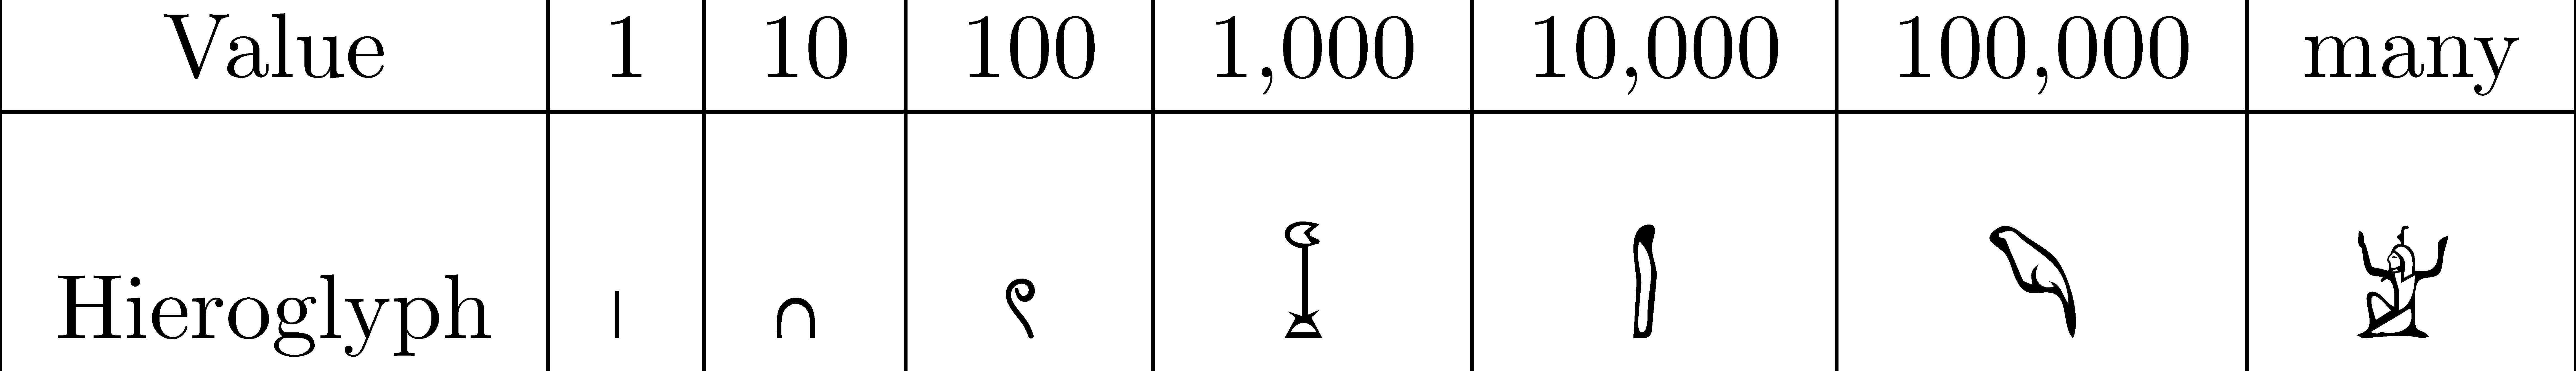
\includegraphics[width=0.9\linewidth]{tikz/hieroglyphs} 

}

\end{figure}

\begin{example}[Roman Numeration]
\protect\hypertarget{exm:unnamed-chunk-61}{}{\label{exm:unnamed-chunk-61} \iffalse (Roman Numeration) \fi{} }The Roman numeration system is similar to the Egyptian system, in that the Roman numbers are each unique to a particular value (for example, X means \(10\)). The Roman system improved on the Egyptian numeration system by imposing an order to how these numbers could be presented and partially solved the potential for a large number of repeated numbers by adding the subtraction element (so, IX would mean take \(1\) away from \(10\), while XI means add one to \(10\)). However, as students of the Super Bowl know, reading these numbers still takes a fair amount of decoding and there is a still a problem with needing a new number for each new grouping.
\end{example}
\begin{table}

\caption{\label{tab:roman}Roman Numeration}
\centering
\begin{tabular}[t]{l|l}
\hline
Arabic Numeral & Roman Numeral\\
\hline
1 & I\\
\hline
10 & X\\
\hline
100 & C\\
\hline
1,000 & M\\
\hline
\end{tabular}
\end{table}

\begin{example}[Base $5$]
\protect\hypertarget{exm:unnamed-chunk-62}{}{\label{exm:unnamed-chunk-62} \iffalse (Base \(5\)) \fi{} }Base \(5\) is like our current standard numeration system, except it uses a set of five digits, \(\{0,1,2,3,4\}\), and place values are based on powers of \(5\), not \(10\). In the United States we use base \(5\) in some of our coins, in that there are \(5\) pennies in a nickel and \(5\) nickels in a quarter. Then the number \(14_{5}\) (read as fourteen base five) is saying \(1\) nickel and \(4\) pennies, or \(9\) cents. Similarly,
\[231_{5} = 2\cdot 5^2 + 3\cdot 5^1 + 1 \cdot 5^0 = 66_{10}.\]
\end{example}

While there is no obvious use for students to learn operations in a different base, working outside of our base 10 system can help teachers recognize and understand the inner workings of the base 10 system and its associated algorithms. As these algorithms are introduced throughout the section, you are encouraged to use the algorithms to perform operations on numbers in these additional base systems.

\begin{example}[Base $12$]
\protect\hypertarget{exm:unnamed-chunk-63}{}{\label{exm:unnamed-chunk-63} \iffalse (Base \(12\)) \fi{} }The duodecimal (base 12) number system is a component of some languages in West Africa and Nepal and is used in our everyday measurements of dozen and gross. A duodecimal system requires twelve digits, \(0,1,2,3,4,5,6,7,8,9,t,e\), and place values are based on powers of \(12\). In this system \(6+5=e\), \(7+8=13\), and
\[3t \times e4 = 2te4.\]

One of the implications of a base 12 system is additional tricks for multiplying numbers due to a larger number of factors of twelve than ten.
\end{example}

\hypertarget{representations-of-number}{%
\subsection{Representations of Number}\label{representations-of-number}}

In talking about numeration systems, we have exclusively been using one form of number representation. However, numeration systems are only one way that we communicate ideas about number. In this section, we explore different ways of representing numbers, each which helps develop different properties of numbers. For this introduction to representation, we focus first on the positive natural numbers, adding additional elements to these representations as we develop the various number systems.

\hypertarget{sets.}{%
\subsubsection*{Sets.}\label{sets.}}
\addcontentsline{toc}{subsubsection}{Sets.}

As discussed in Chapter \ref{ch:equivalence}, we can think of 3 as an equivalence class for all sets containing 3 objects. (We will go into this in more detail in Section \ref{sec:cardinality}.) As such, sets can be used to represent numbers, either pictorially as a circle containing generic objects or as a set with general elements. Using sets offers the most general representation of number we can develop, as it does not impose any structure on the representation beyond the property of ``how many''. Relationships between numbers (such as inequality or equality) are fairly straightforward to model, but comparing a large number at one time would be difficult using this representation. As a result, most middle and high school textbooks do not represent numbers this way, although it is fairly common in the elementary grades.

\begin{figure}

{\centering 
\includegraphics[width=0.2\linewidth]{tikz/Set-representations} 

}

\end{figure}

or \(\{a,b,c\}\).

\hypertarget{number-line.}{%
\subsubsection*{Number Line.}\label{number-line.}}
\addcontentsline{toc}{subsubsection}{Number Line.}

The number line imposes more structure on the number representation than the use of sets. In particular, it organizes numbers along a line, with integers spaced evenly along the line. This representation allows multiple numbers to be visualized at the same time while also showing relationships between the numbers represented. In this representation, any number that falls at the location of 3 is equivalent to three. Numbers of the left of 3 are less than it, while numbers above are greater.

\begin{figure}

{\centering 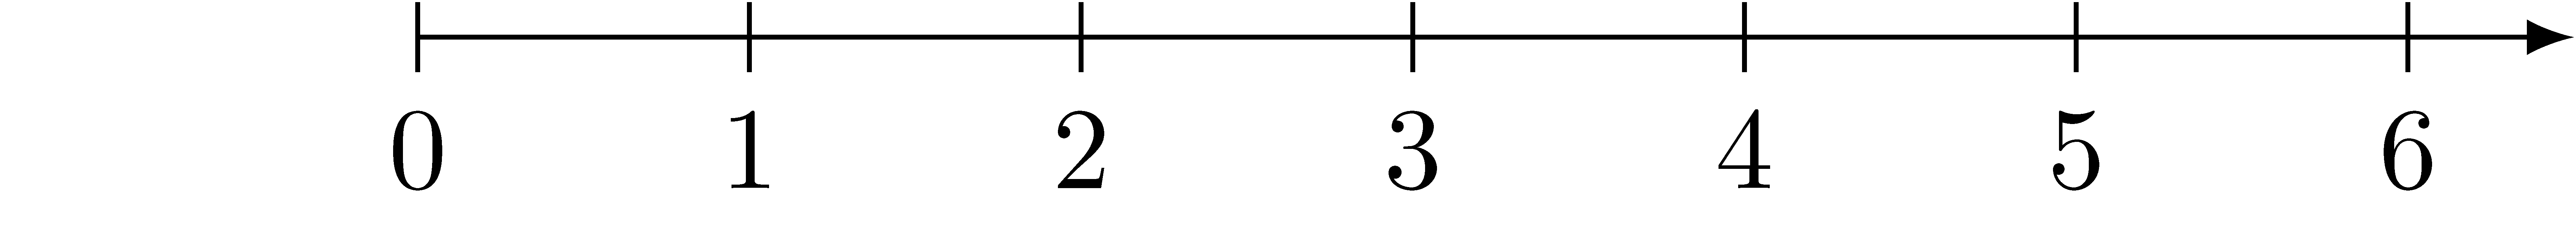
\includegraphics[width=0.8\linewidth]{tikz/number-line-representation} 

}

\end{figure}

\hypertarget{base-10-blocks.}{%
\subsubsection*{Base-10 Blocks.}\label{base-10-blocks.}}
\addcontentsline{toc}{subsubsection}{Base-10 Blocks.}

Base-10 blocks are usually a physical way (although virtual and pictorial versions exist) to represent numbers specifically designed to promote understanding of place value. The blocks come in four sizes: units (small, approximately 1-centimeter cubes), rods (10, represented by a stack of 10 unit cubes), flats (100, represented by a 10 by 10 grid of unit cubes), and big cubes (1000, represented by a cube with side lengths equal to 10 unit cubes). Representing a number using base-10 blocks means drawing or collecting the correct number of blocks for each place value.

\begin{figure}

{\centering 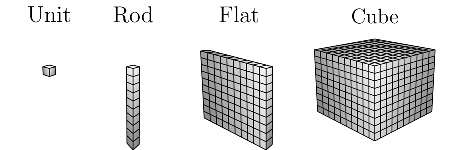
\includegraphics[width=0.8\linewidth]{tikz/base10blocks} 

}

\end{figure}

In order to write down the reasoning these blocks are sometimes transitioned into dots, lines, and squares. So that \(13+24\) is represented by

\begin{figure}

{\centering 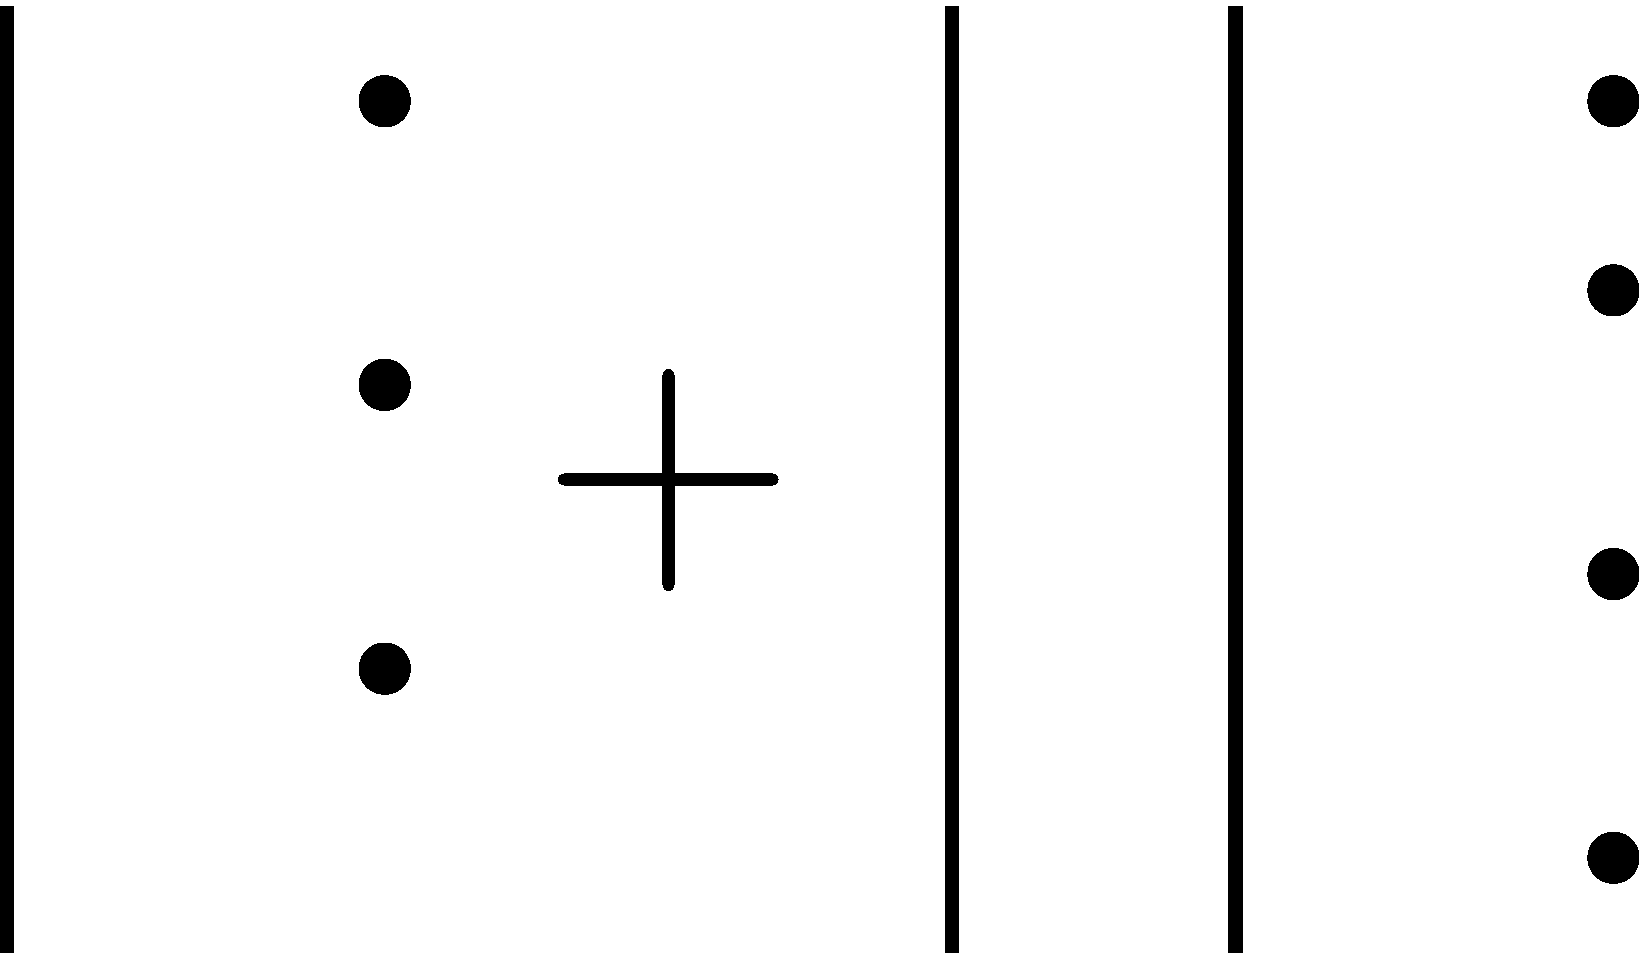
\includegraphics[width=0.6\linewidth]{tikz/base10block-addition} 

}

\end{figure}

\hypertarget{cuisenaire-rods.}{%
\subsubsection*{Cuisenaire Rods.}\label{cuisenaire-rods.}}
\addcontentsline{toc}{subsubsection}{Cuisenaire Rods.}

Cuisenaire rods are another physical way that numbers are represented. They are a collection of long prisms of different colors and lengths. Rods of the same length are the same color, and each length is a natural number multiple of the smallest rod. These rods are used for a variety of reasons including factoring of natural numbers, but one of the most common is to help students understand concepts related to rational numbers and the operation of division.

\begin{figure}

{\centering 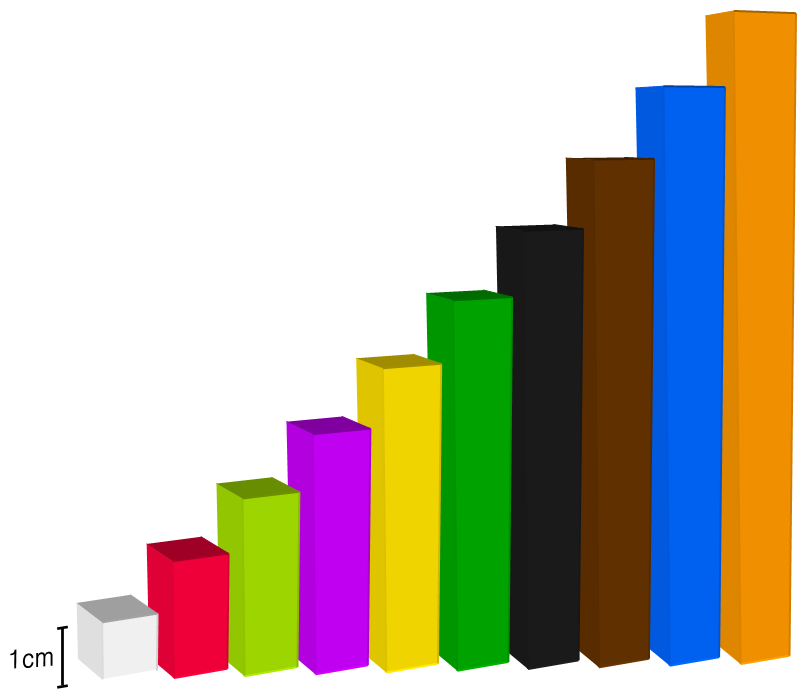
\includegraphics[width=0.3\linewidth]{images/Cuisenaire-Rods-2} 

}

\caption{Cuisenaire Rods}\label{fig:unnamed-chunk-68}
\end{figure}

\hypertarget{addition-models-and-algorithms}{%
\subsection{Addition Models and Algorithms}\label{addition-models-and-algorithms}}

Much like the concept of number, it is easy to overlook how quickly addition becomes a complex endeavor for young students of mathematics. Fundamentally, addition represents the notion of ``combine'' or finding the union of mutually disjoint sets.

\begin{figure}

{\centering 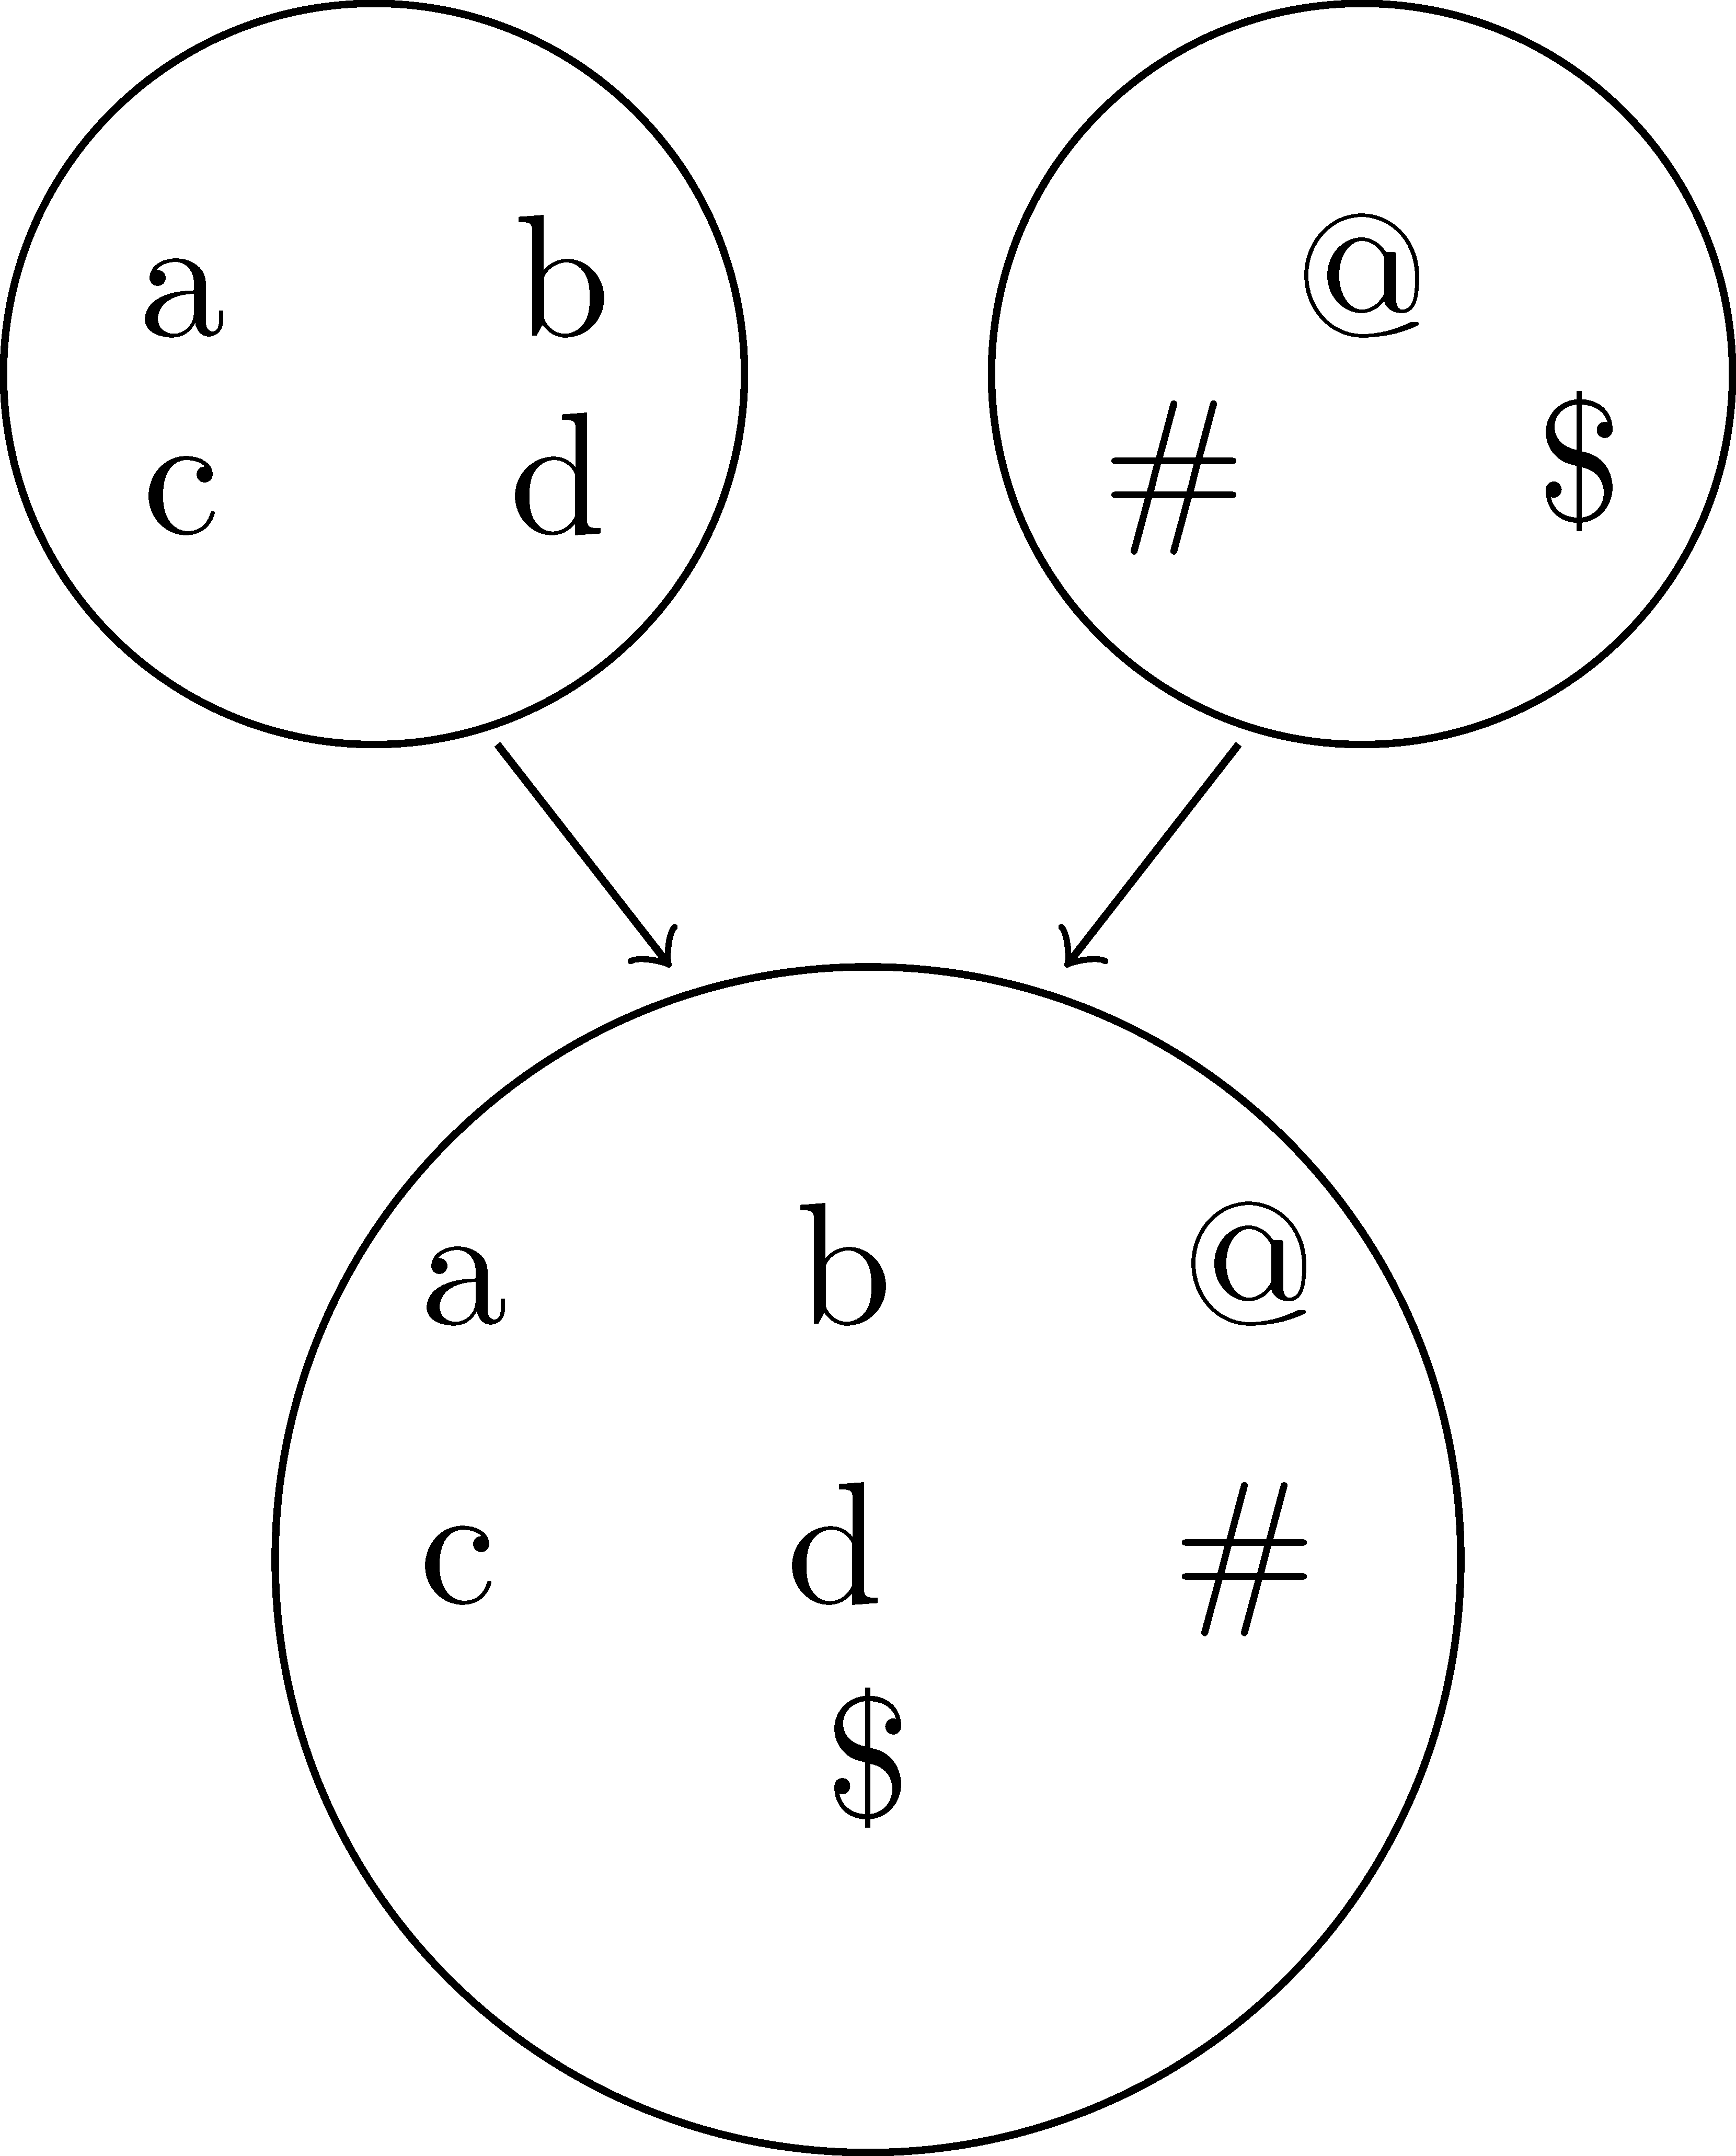
\includegraphics[width=0.3\linewidth]{tikz/addition-model-set} 

}

\end{figure}

Typically, we quickly move away from representing addition using sets and instead use the number line. For natural number addition, this process is fairly straight forward: Students start by identifying the first addend. Then, count up the number that is being added. The number you land on is the result.

\begin{figure}

{\centering 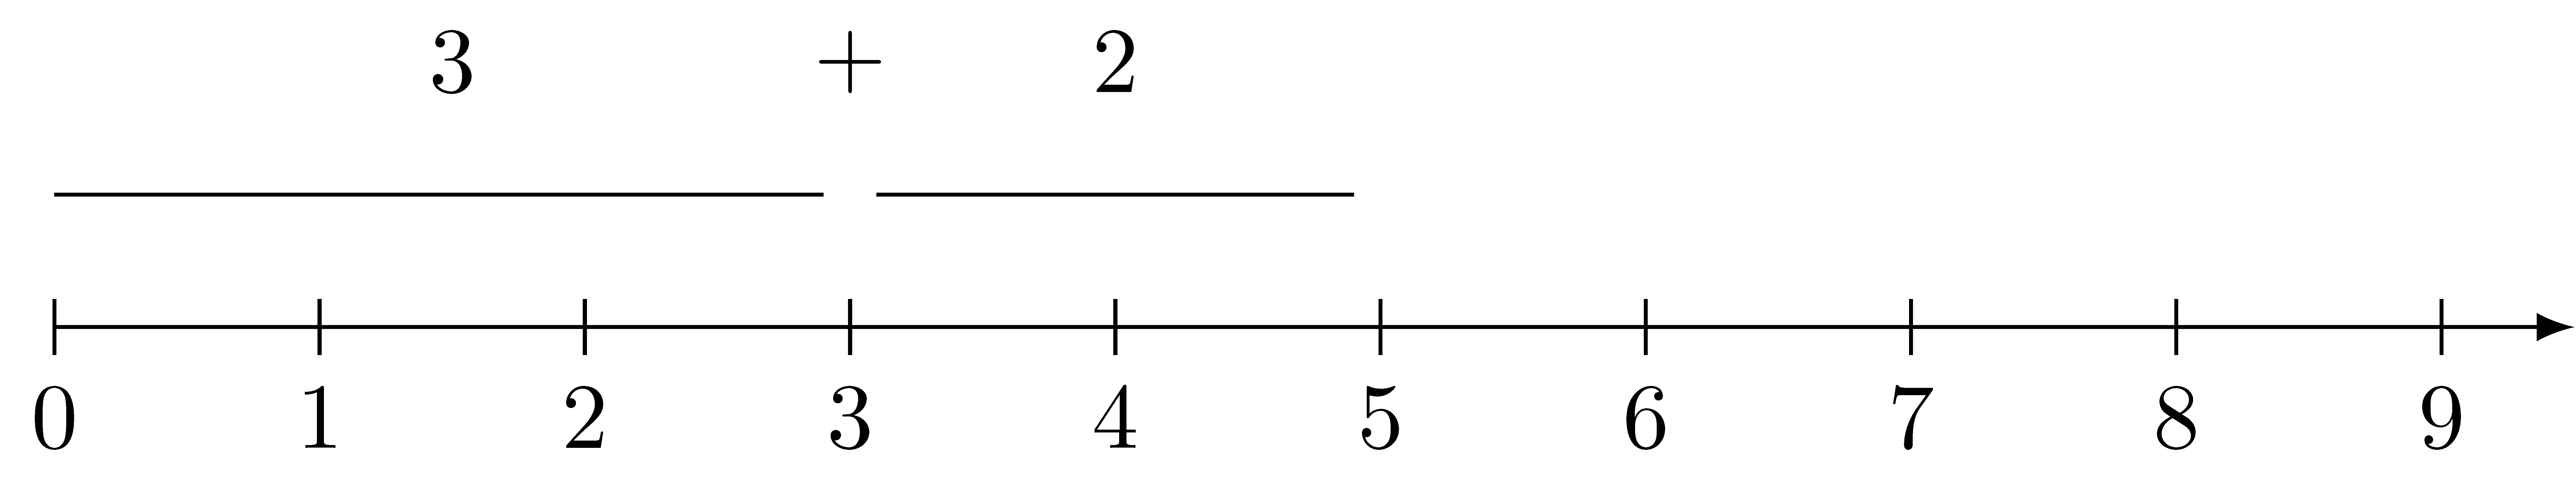
\includegraphics[width=0.6\linewidth]{tikz/addition-model-numberline} 

}

\end{figure}

Thinking of addition as the union of sets or on a number line of the natural numbers are good, conceptual starting places for understanding addition. However, doing so will lead some students to think that ``when two numbers are added, the result will be the same size or bigger.'' In the natural numbers this thinking will work, but in the integers the reasoning begins to fall apart. Note that idea of ``combine'' does not say anything about the size of the result relative to the others, so the common error is a result of students focusing on the result rather than the concept of addition.

When asked to add something like \(125+258\) without the use of a calculator, most adults are well-trained to rewrite the sum and apply the standard algorithm.

\begin{figure}

{\centering 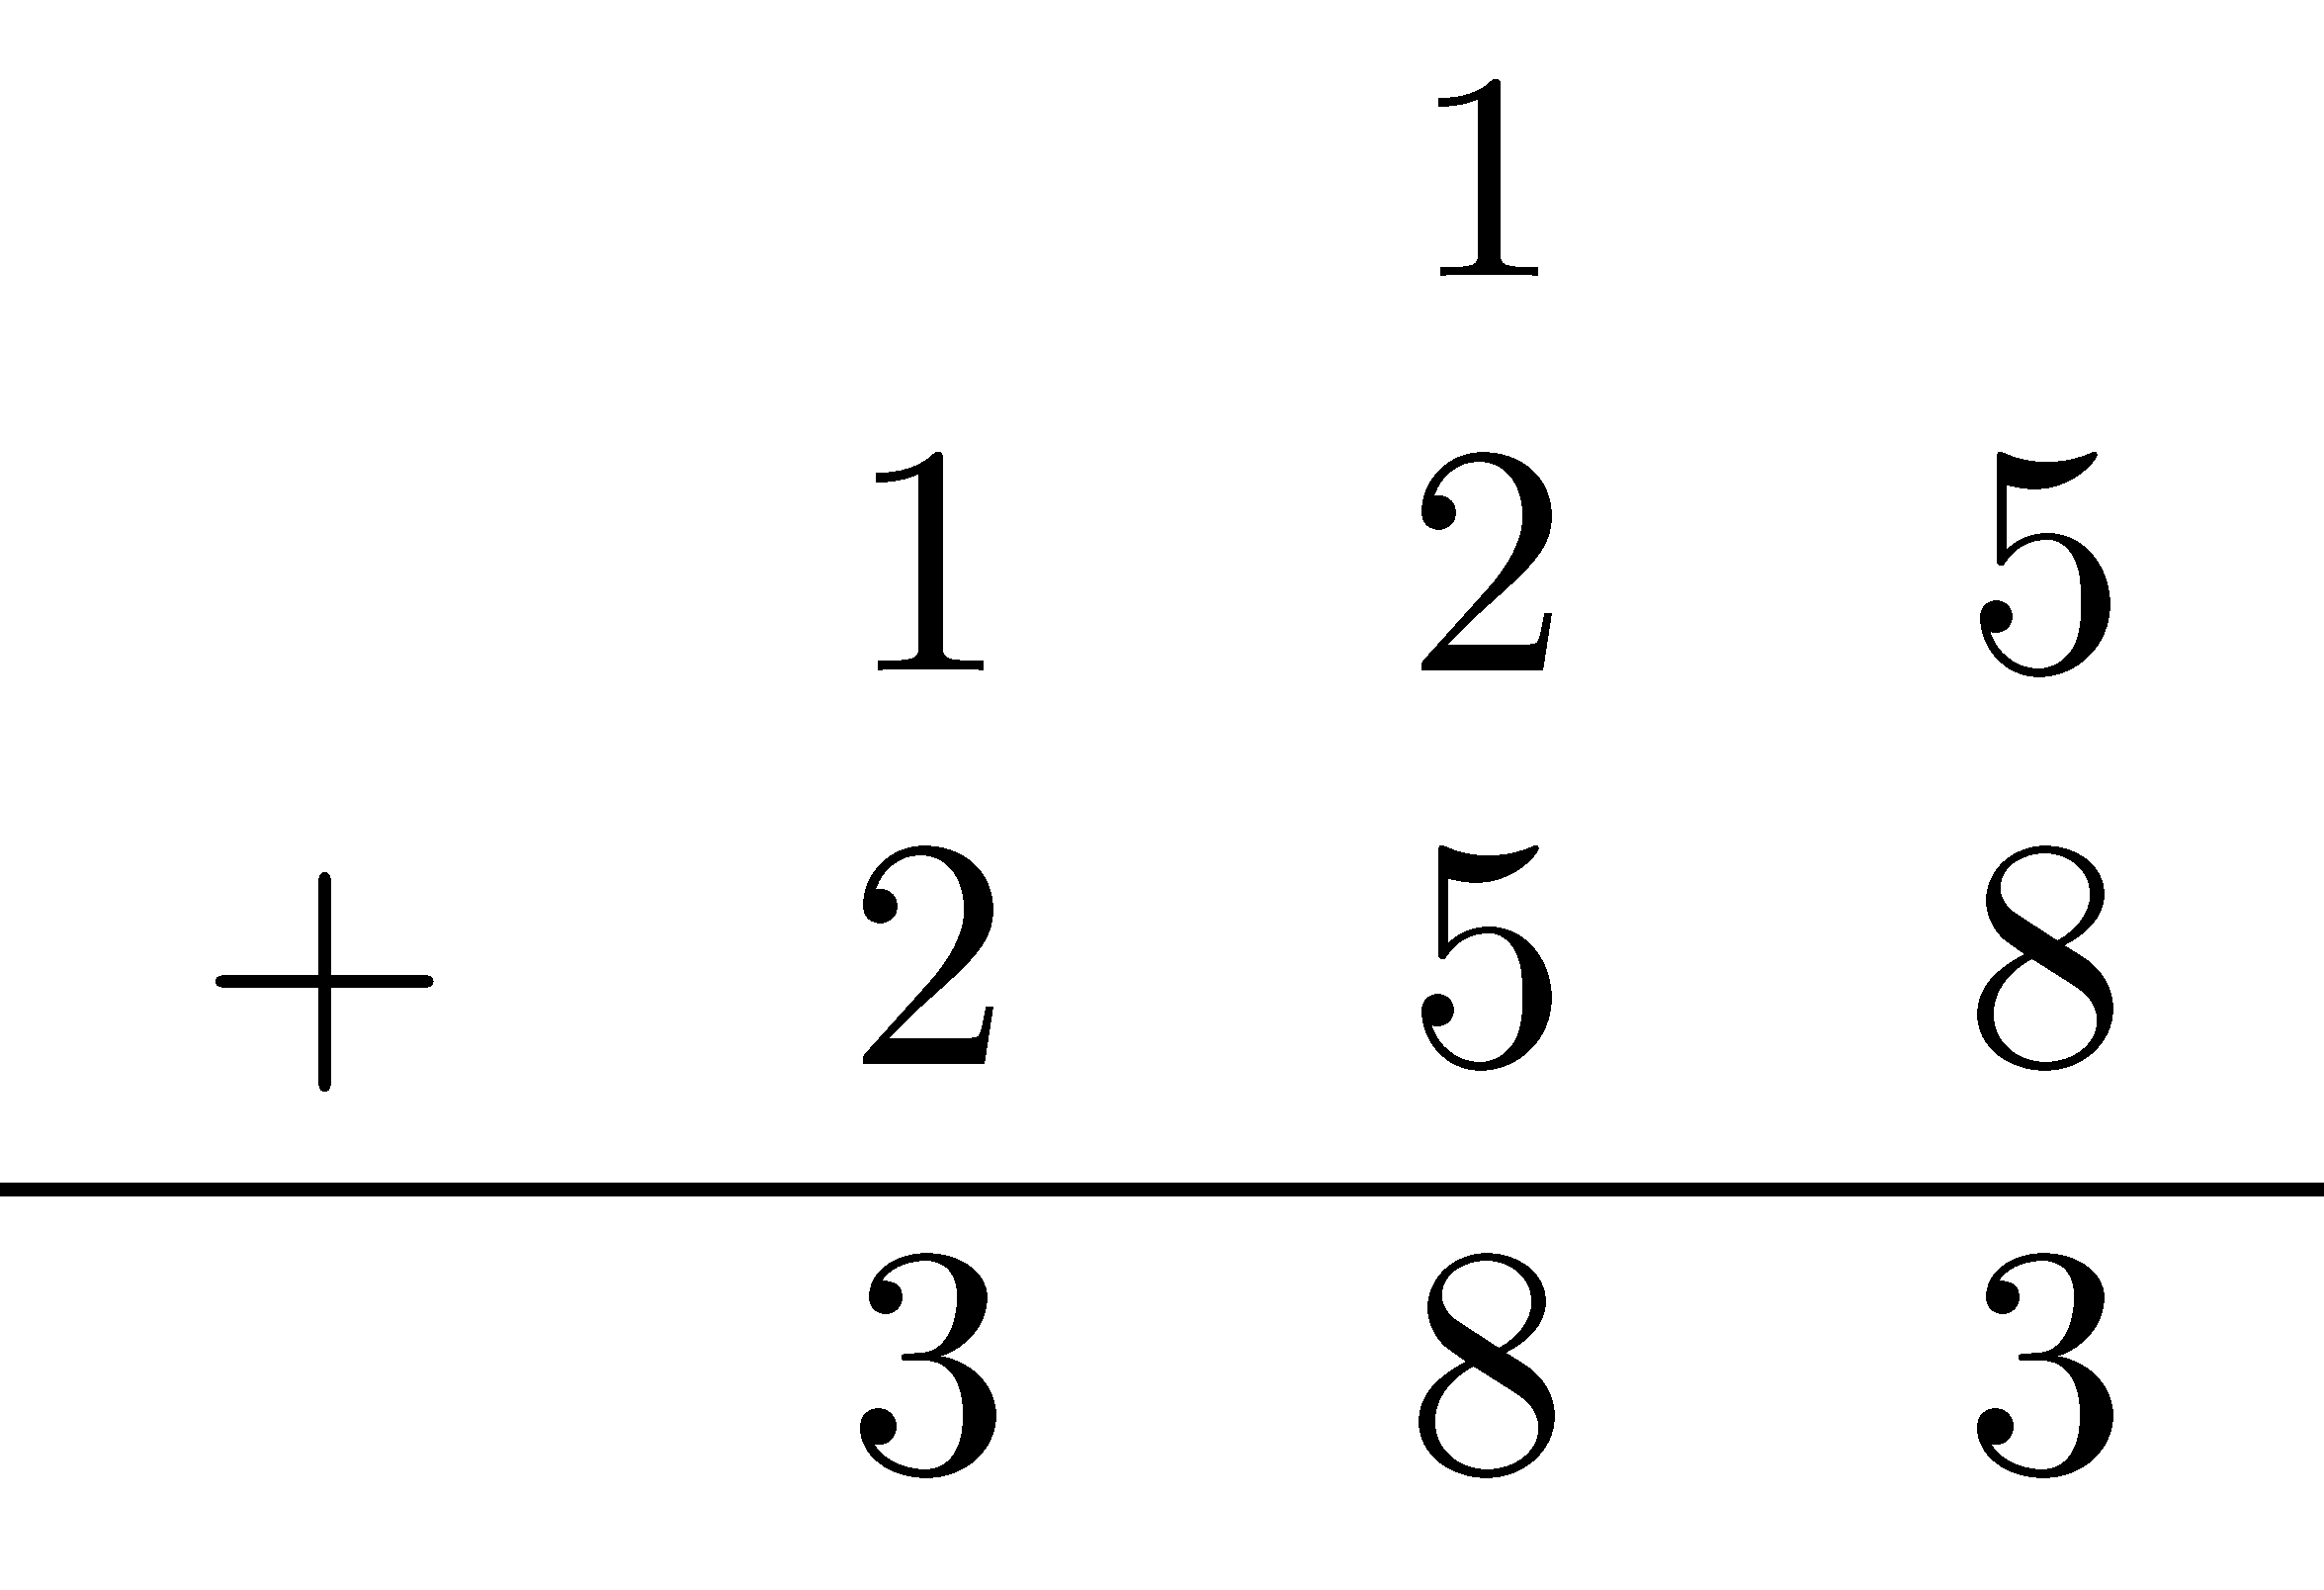
\includegraphics[width=0.2\linewidth]{tikz/addition-model-algorithm} 

}

\end{figure}

While the work of teaching children these algorithms is usually done in elementary school, it is worth taking a little time to appreciate the ways these traditional methods take advantage of the properties of natural numbers to allow for quick and efficient calculation. To facilitate this discussion, we present several alternative algorithms. It is not our goal to instruct our readers in each of these algorithms: there is not a way to present all possible ways an addition problem can be solved. Rather, we choose algorithms that maximize the opportunity to explore the hidden work of the standard algorithm. A mathematics teacher who studies these examples in relation to the standard algorithm should be able to teach themselves unfamiliar algorithms that they encounter in the wild. For each of these, we use the example \(125+258\).

\hypertarget{expanded-form.}{%
\subsubsection*{Expanded form.}\label{expanded-form.}}
\addcontentsline{toc}{subsubsection}{Expanded form.}

We can rewrite our numbers using place value as \((100+20+5)\) and \((200+50+8)\) and then use associative and commutative properties of addition for the natural numbers.

\begin{align*}
    125+258 &= (100+20+5) + (200+50+8) \\
    &= (100+200) + (20+50) + (5+8)  \\
    &= (100+200) + (20+50) + (13) \\
    &= (100+200) + (20+50) + (10 + 3) \\
    &= (100+200) + (20+50+10) + (3) \\
    &= 300 + 80 + 3 =383 \\
\end{align*}

\hypertarget{lattice-algorithm.}{%
\subsubsection*{Lattice Algorithm.}\label{lattice-algorithm.}}
\addcontentsline{toc}{subsubsection}{Lattice Algorithm.}

The lattice algorithm described below provides another method of adding two numbers by keeping track of place value through some implicit methods.

\begin{itemize}
\tightlist
\item
  Stack the two numbers so that corresponding place values are in the same column. Draw the traditional equals bar.
\end{itemize}

\begin{figure}

{\centering 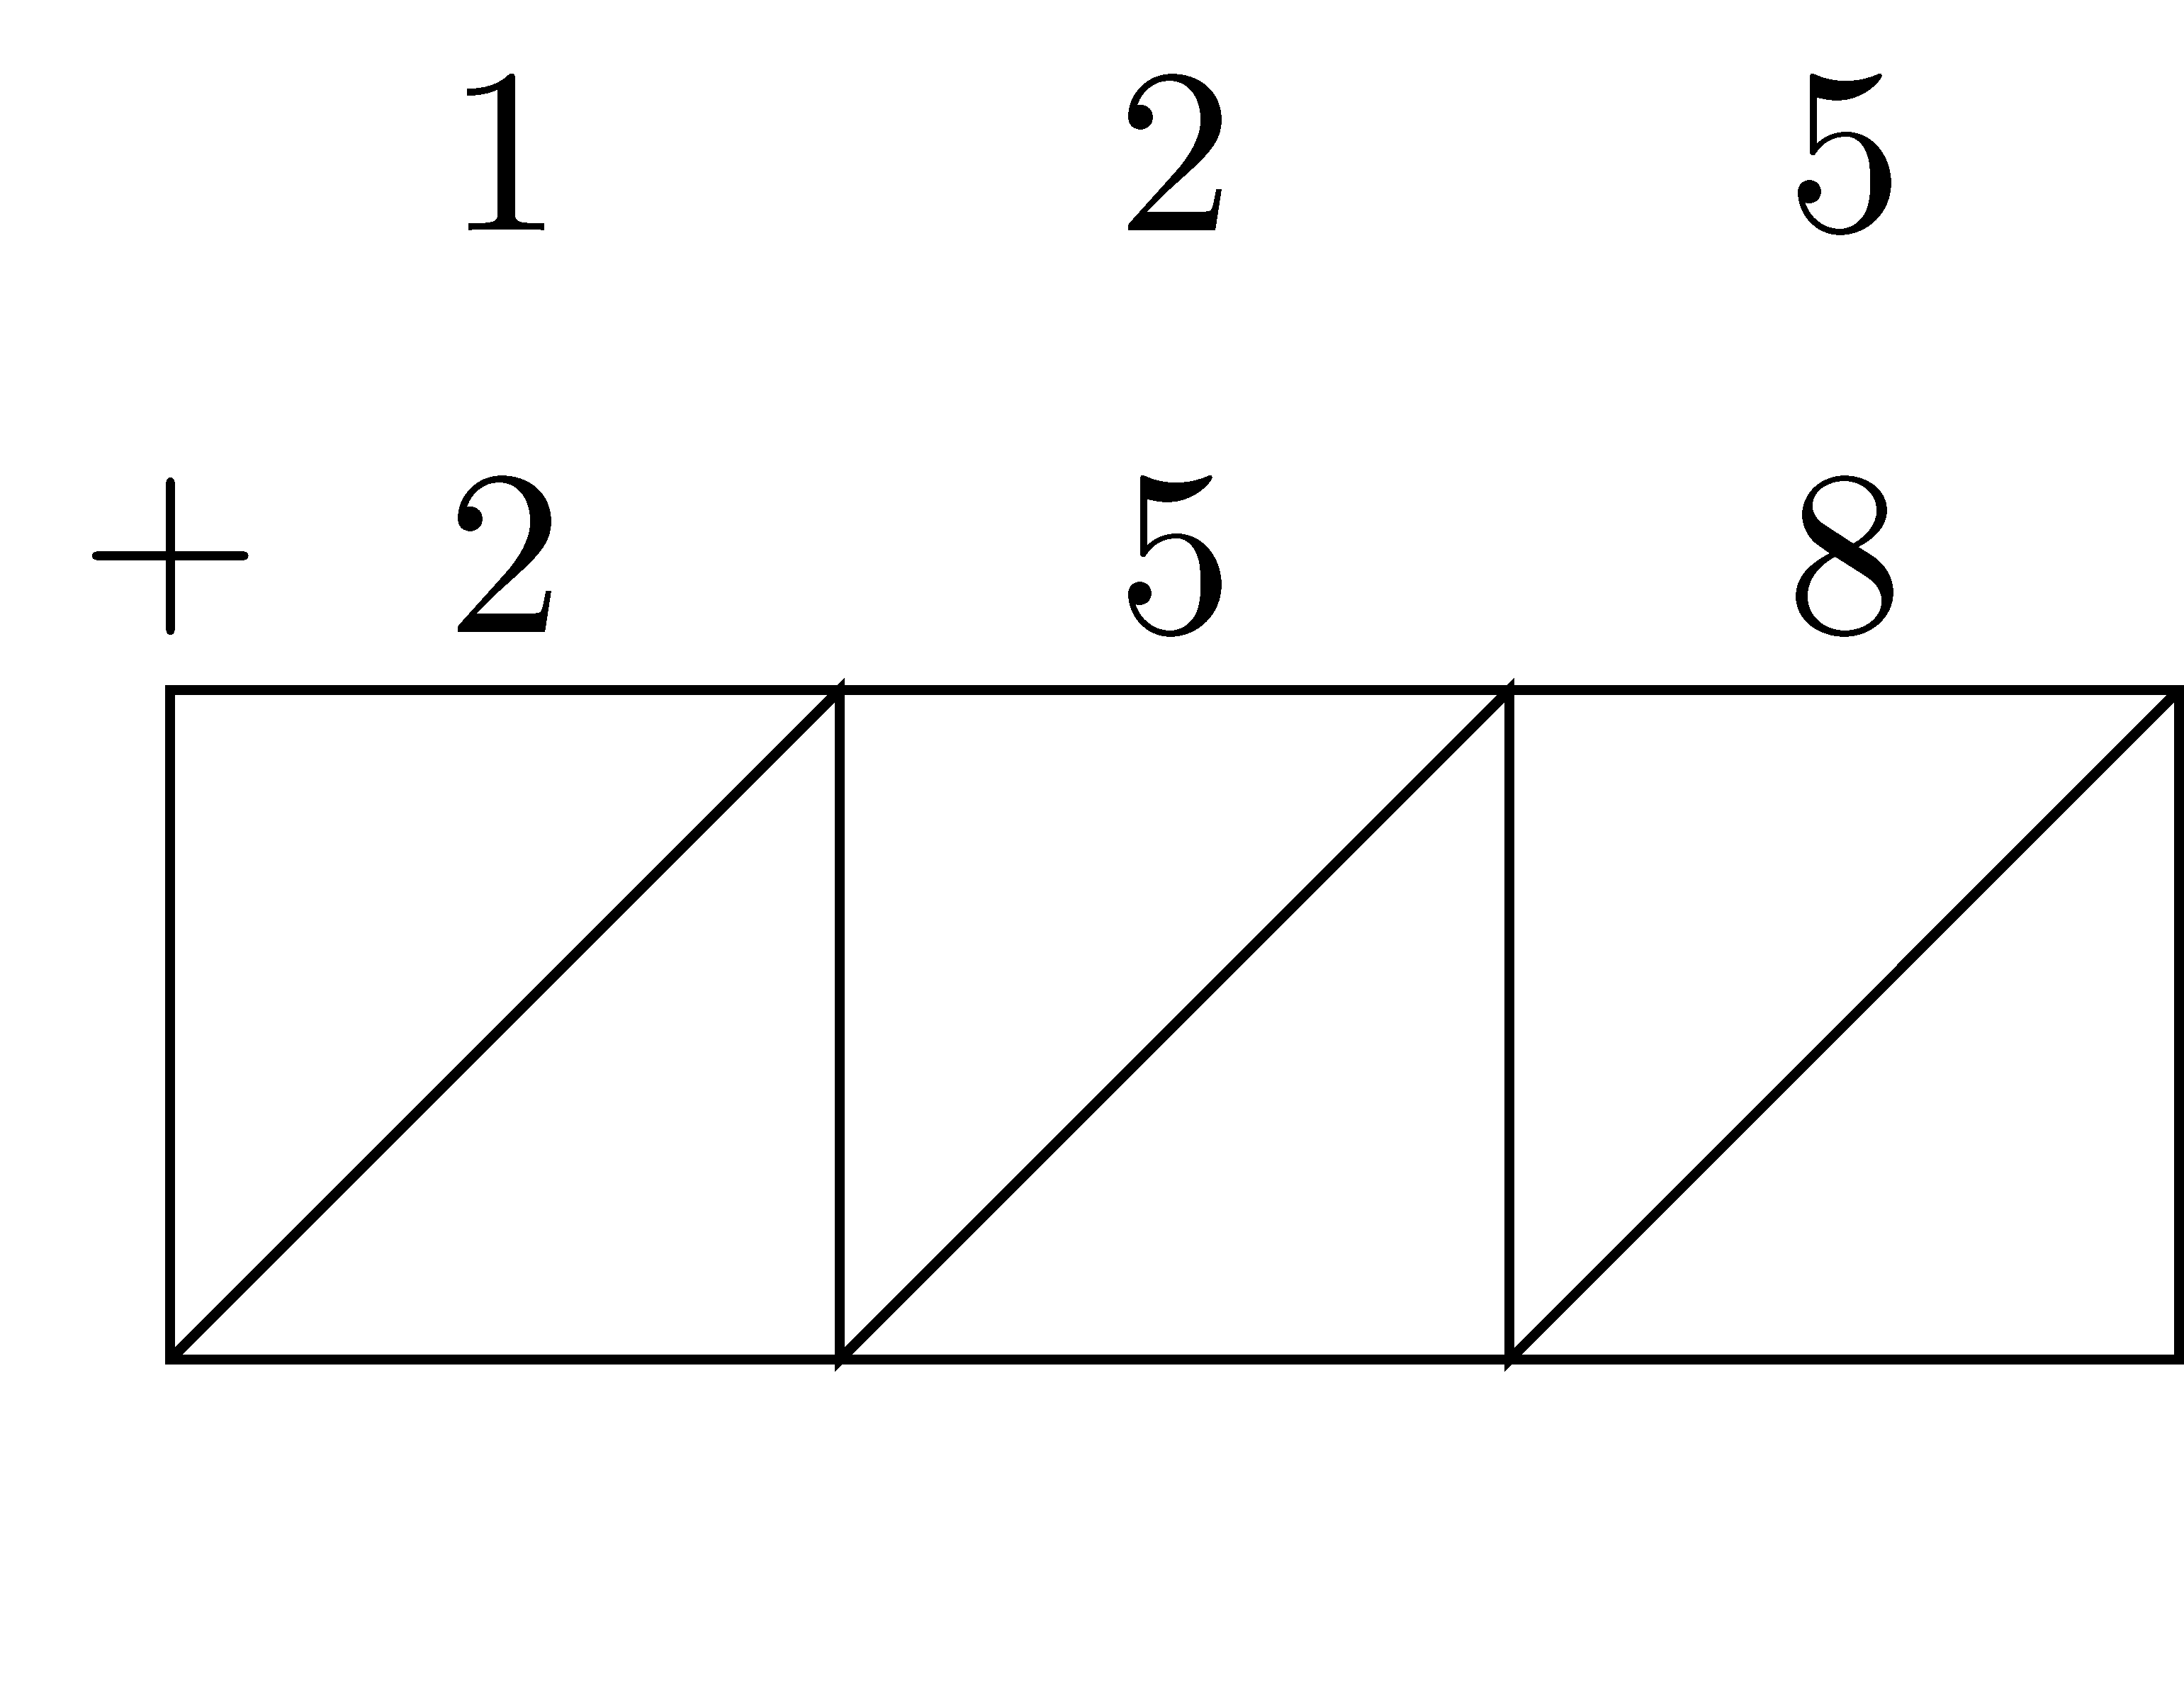
\includegraphics[width=0.2\linewidth]{tikz/lattice-addition1} 

}

\end{figure}

\begin{itemize}
\tightlist
\item
  Starting with the right-most column, add within each column. The result of the digit addition will be a number between 0 and 19. The resulting number is written into the square below the column, with the higher place value going into the higher triangle.
\end{itemize}

\begin{figure}

{\centering 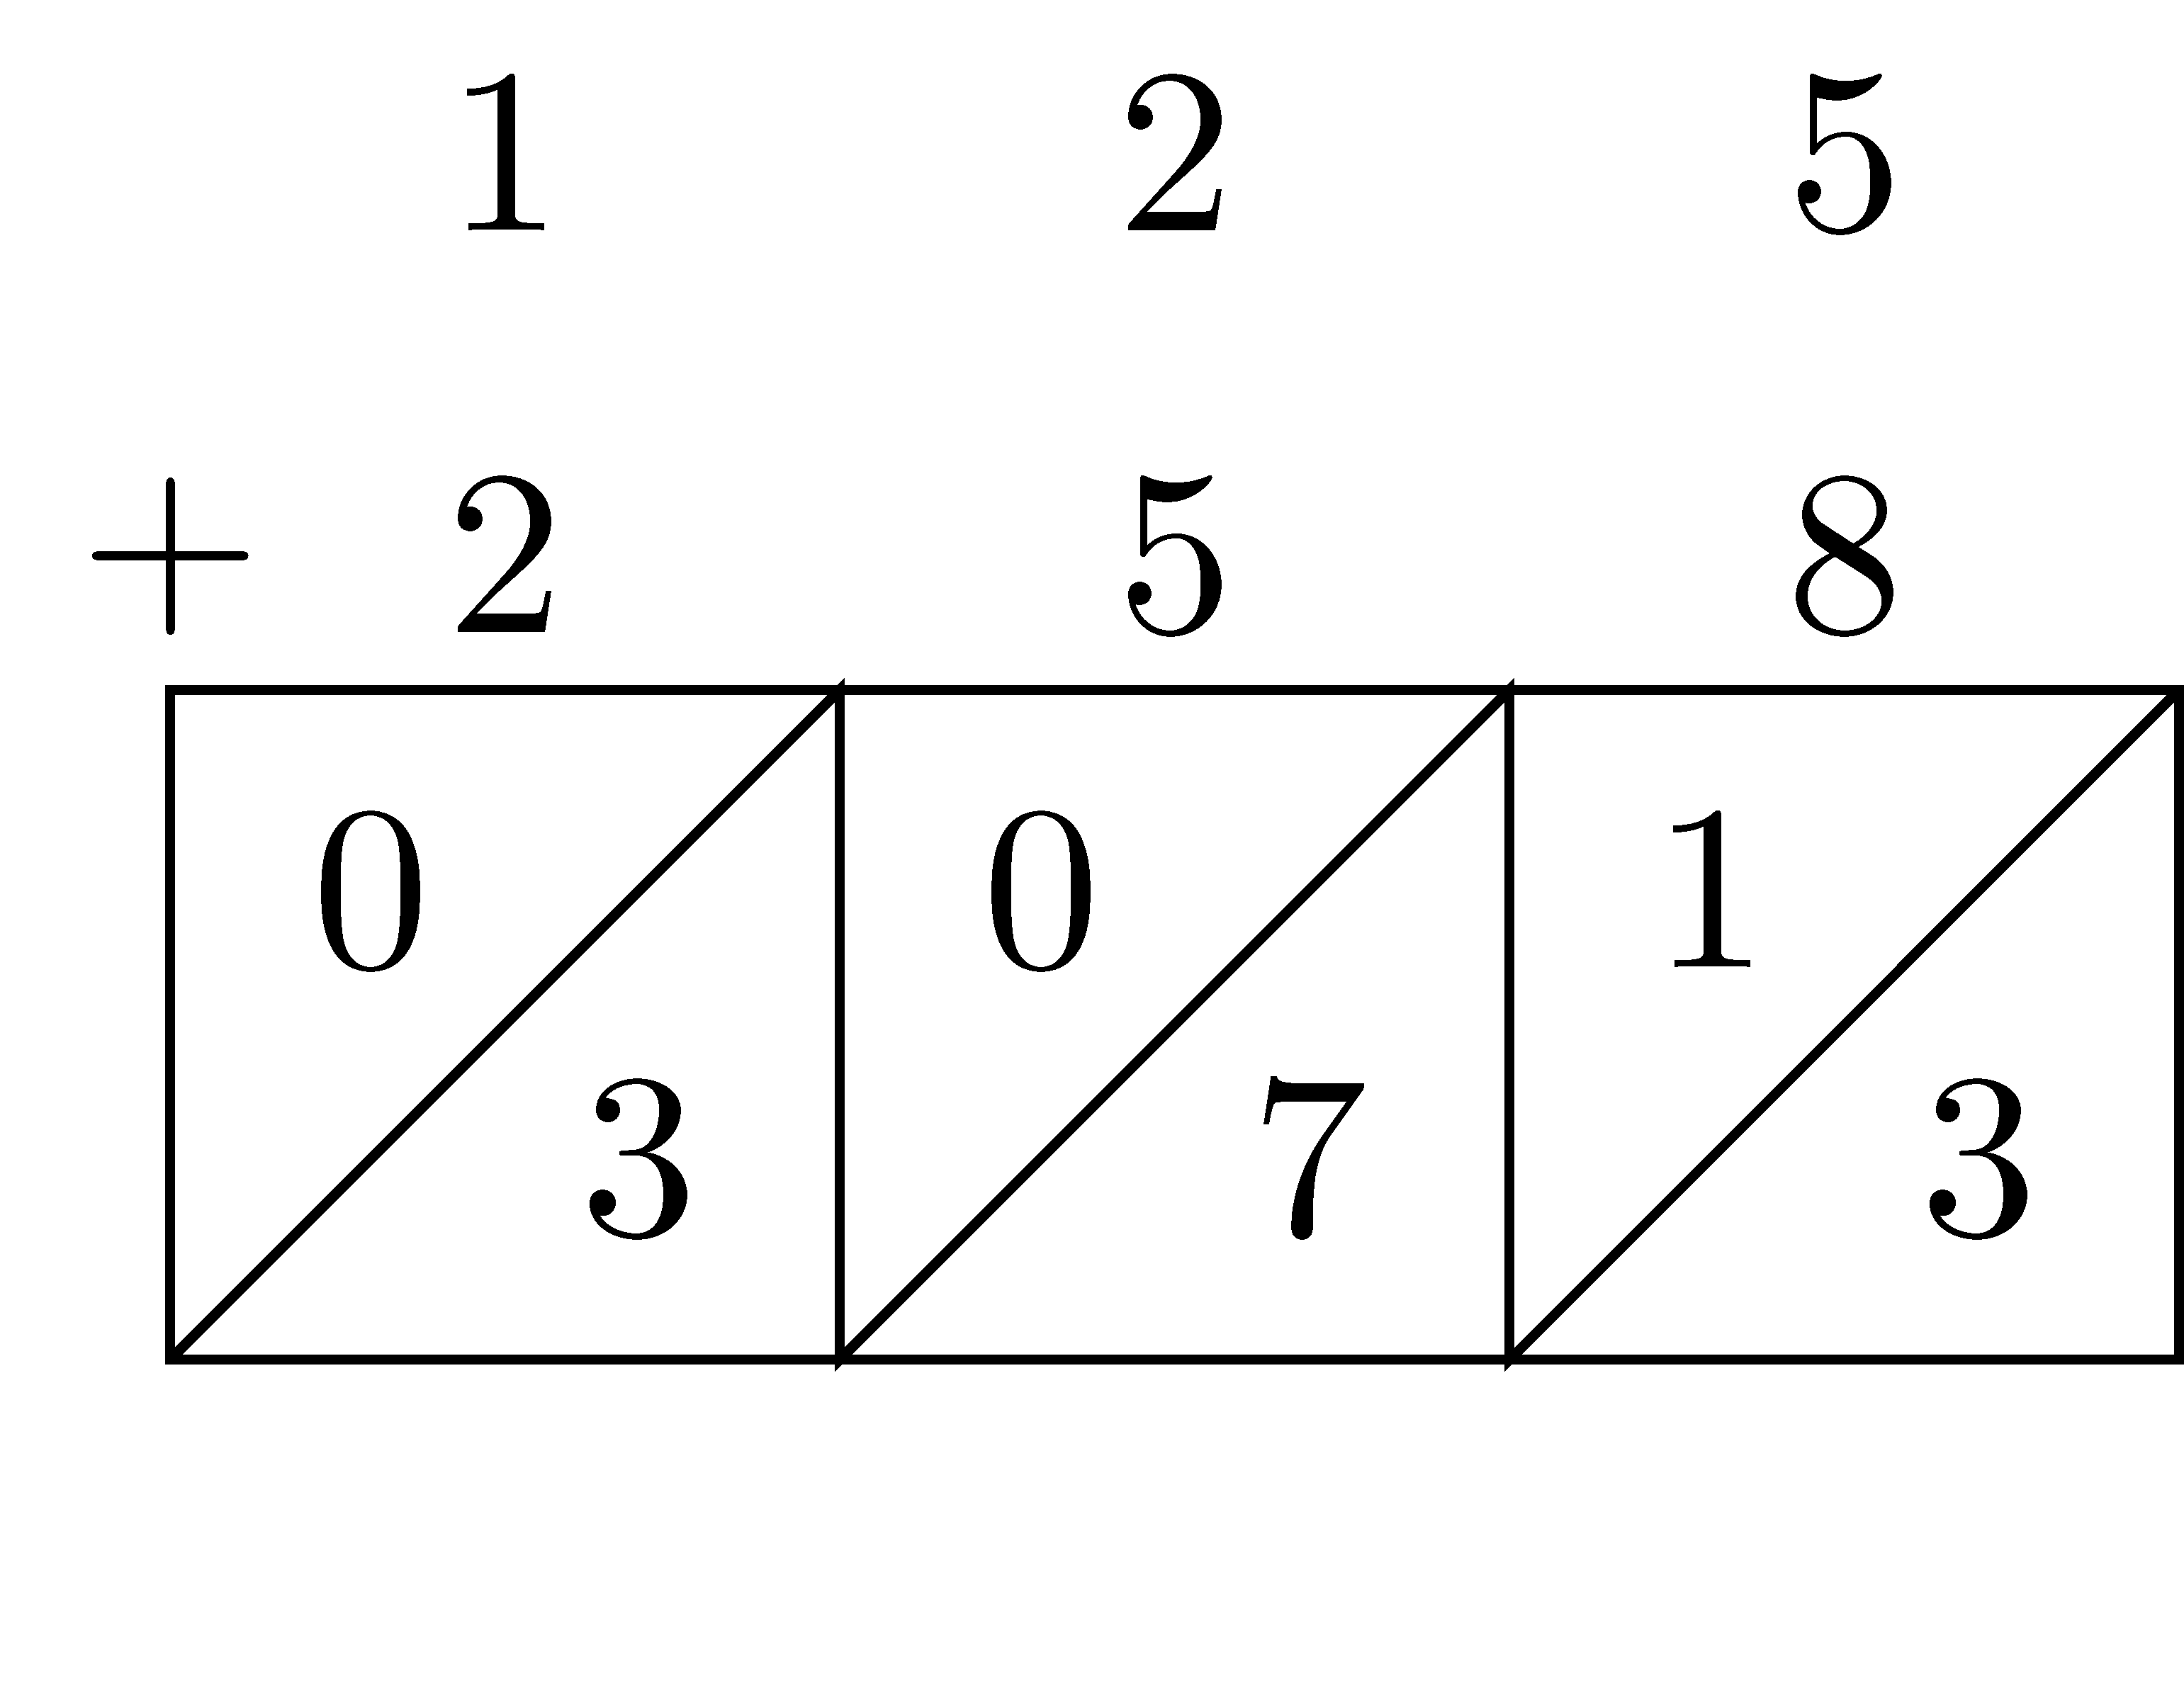
\includegraphics[width=0.2\linewidth]{tikz/lattice-addition2} 

}

\end{figure}

\begin{itemize}
\tightlist
\item
  Add down each diagonal. You are in effect adding the total number of items in each place value.
\end{itemize}

\begin{figure}

{\centering 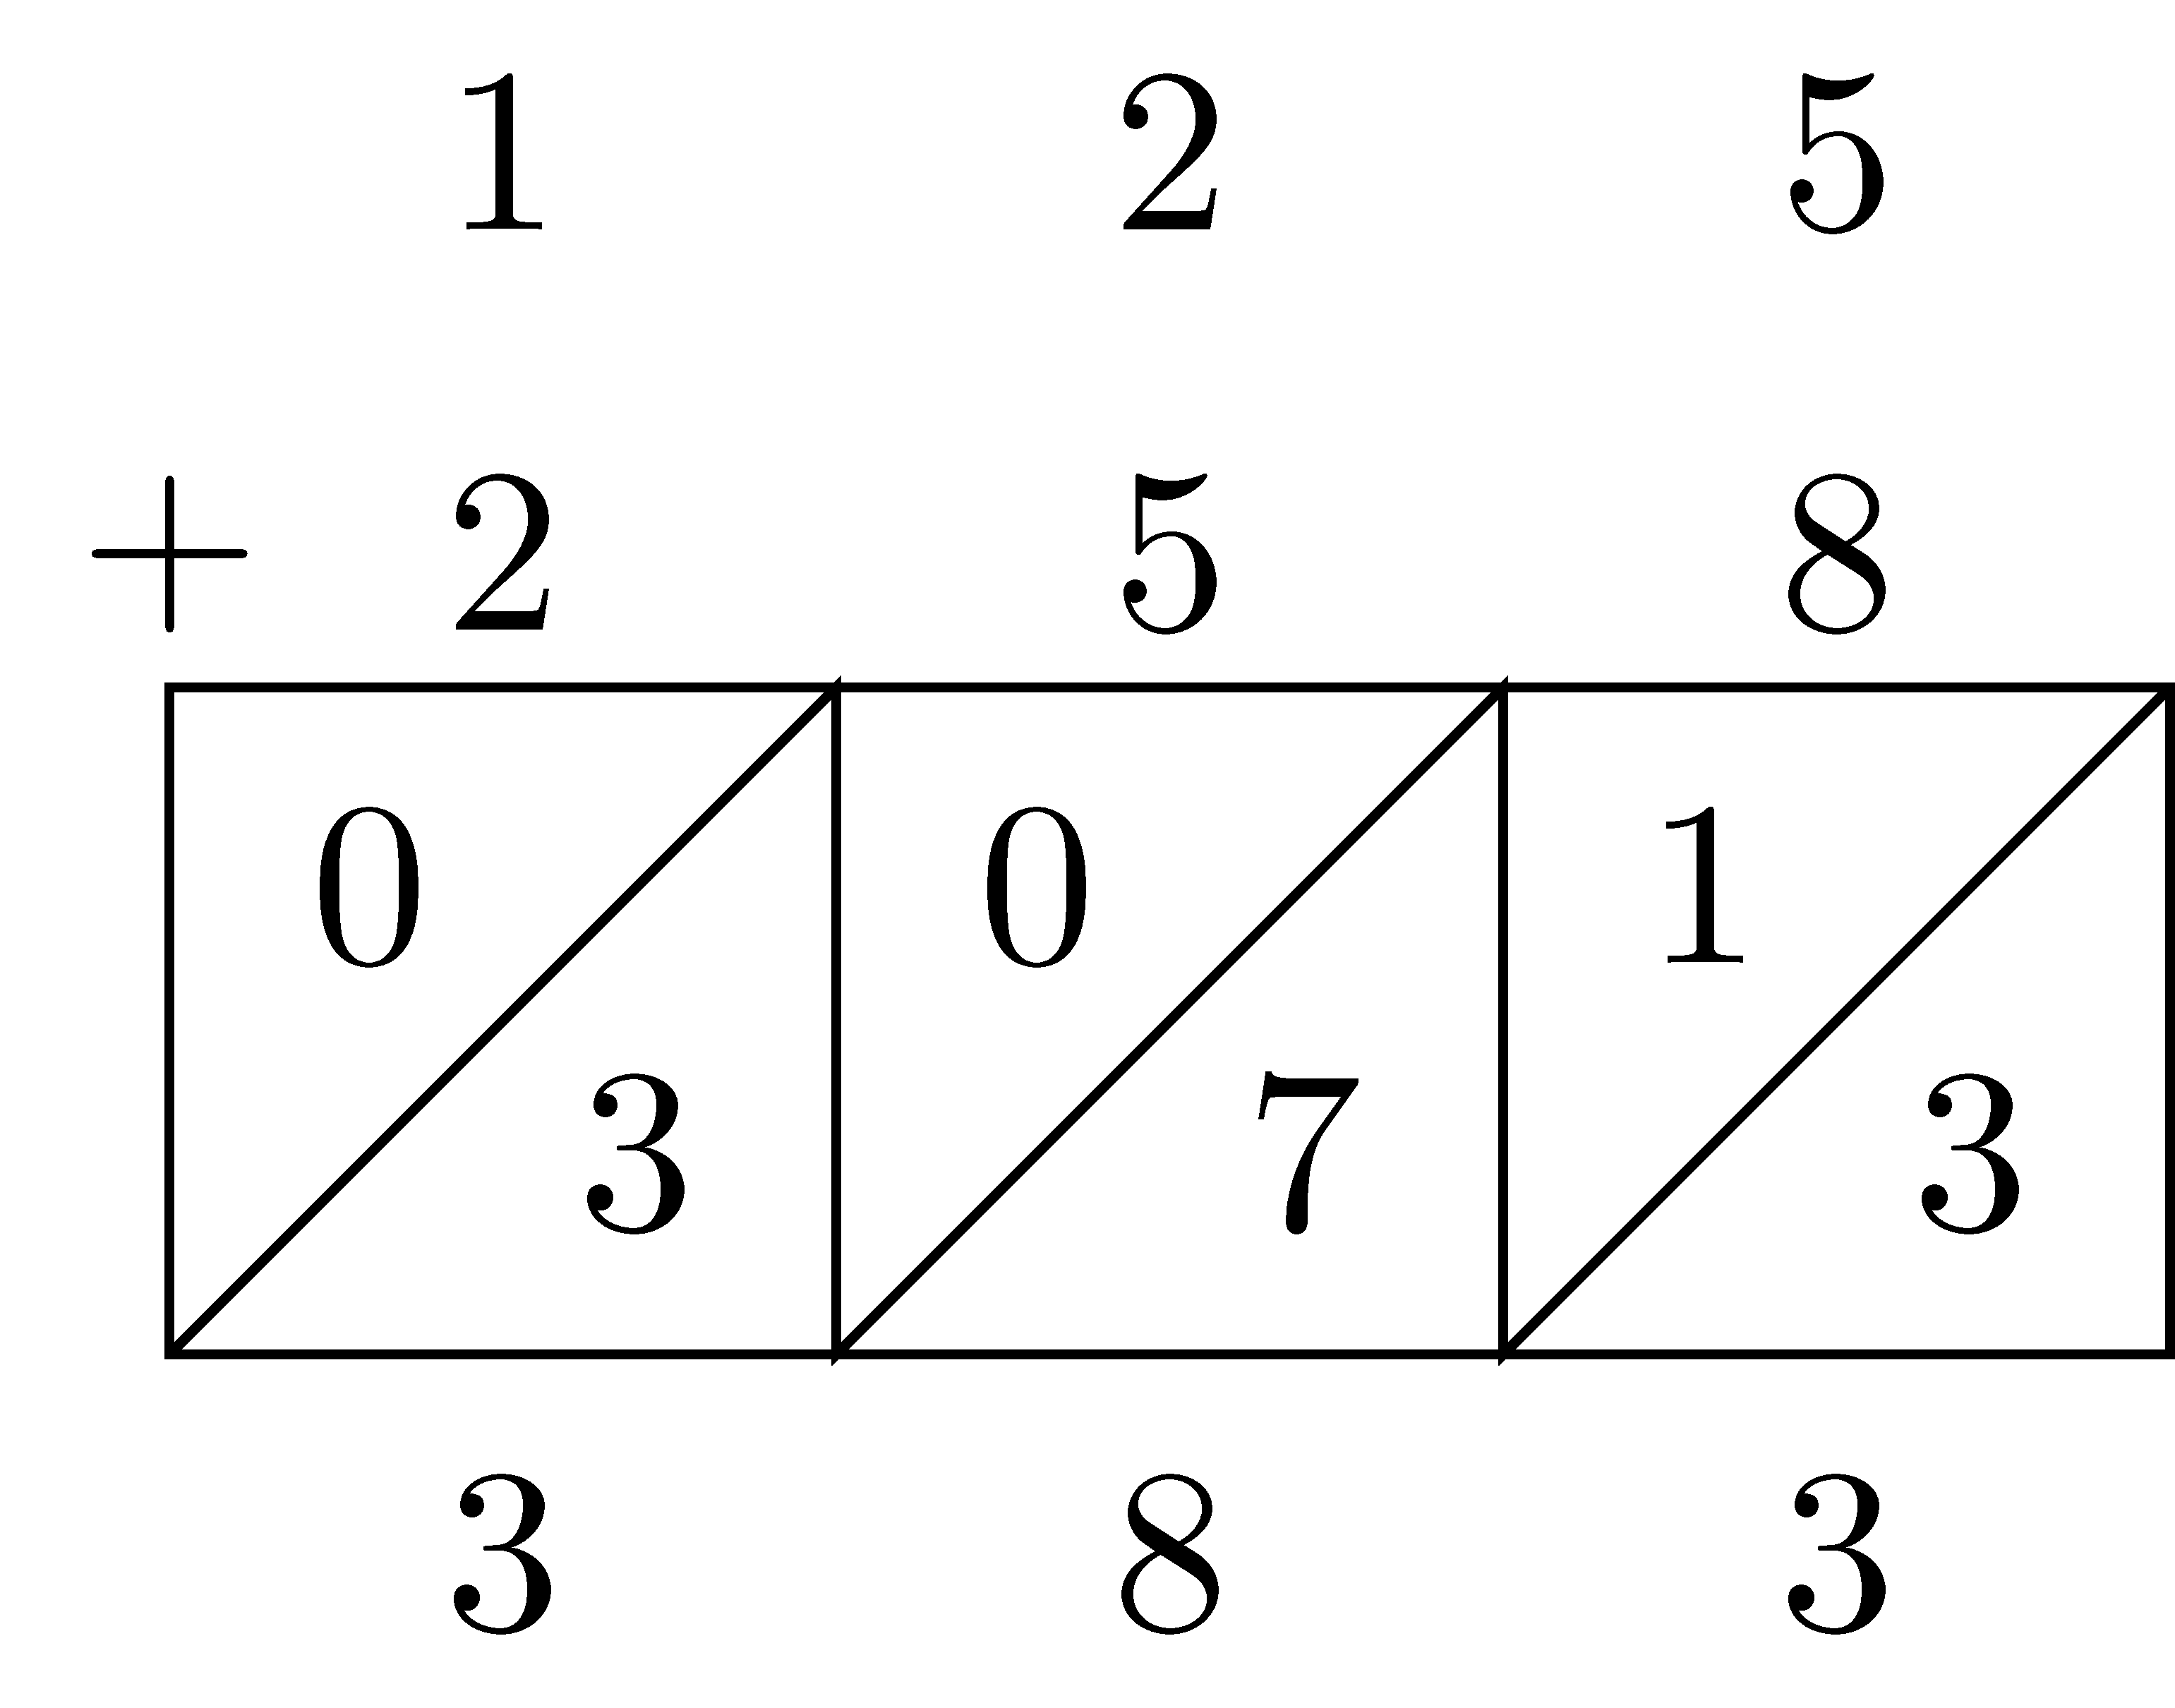
\includegraphics[width=0.2\linewidth]{tikz/lattice-addition3} 

}

\end{figure}

\hypertarget{expanded-algorithm.}{%
\subsubsection*{Expanded algorithm.}\label{expanded-algorithm.}}
\addcontentsline{toc}{subsubsection}{Expanded algorithm.}

The expanded algorithm makes the implicit structure of the lattice algorithm more explicit.

\begin{figure}

{\centering 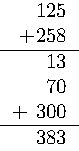
\includegraphics[width=0.1\linewidth]{tikz/addition-model-algorithm-expanded} 

}

\end{figure}

You may have noticed that regardless of which method we used, there were several common elements that all of the algorithms created in one form or another. Perhaps most obviously, \(13\) occurred in all three calculations. The intermediate sums an algorithm produces are called \textbf{partial sums}. Note that although every algorithm used partial sums, they are not always the same between algorithms, even for the same addition problem. These differences in partial sums are a result of where the algorithm does the \textbf{regrouping} of the partial sums. Regrouping, generally, is the process of converting numbers expressed in terms of one place value into a different place value. For example, in the standard algorithm example at the beginning of this section, we got \(13\) when we added the ones digits in the right most column. Since \(13\) ones is not useful for continued adding, we regrouped \(13\) as \(1\) ten and \(3\) ones. We wrote the \(3\) in the ones place value and the \(1\) above the \(10\)'s place value column. You may have learned this process by the name of ``carrying the one''. This language is no longer encouraged in teaching as it masks the fact that the value of the one changes as a person works through every place value.

\hypertarget{subtraction-models-and-algorithms}{%
\subsection{Subtraction Models and Algorithms}\label{subtraction-models-and-algorithms}}

Conceptually, we described addition as the process of combining. Subtraction has two different physical interpretations: the process of removal (often referred to as taking away) or the inverse operation of addition. These are clearly related, but are developed separately, which we explore a bit more in the following paragraphs. Although both interpretations of subtraction seem straight forward when modeled in the physical world, students struggle with this operation a great deal more than addition. This may be at least partially because while the natural numbers have some great properties under addition (closed, commutative, and associative) that make addition easy to set up, but none of these properties under subtraction.

Using our different representations, we can model subtraction a couple different ways: the take away model or the missing addend model.

\hypertarget{take-away-model.}{%
\subsubsection*{Take-Away Model.}\label{take-away-model.}}
\addcontentsline{toc}{subsubsection}{Take-Away Model.}

The first interpretation of subtraction is as removal or the process of taking away. In the mathematics education literature, this is called the ``take-away model''. This conceptualization of subtraction is a direct interpretation of the calculation \(a-b\), where the translation of this expression is ``\(a\) take away \(b\).''

To model \(a-b\) using sets and the take-away model, we start with a set containing \(a\) elements and remove \(b\) elements from it. The composition of the set after the removal process is the resulting difference.

\begin{figure}

{\centering 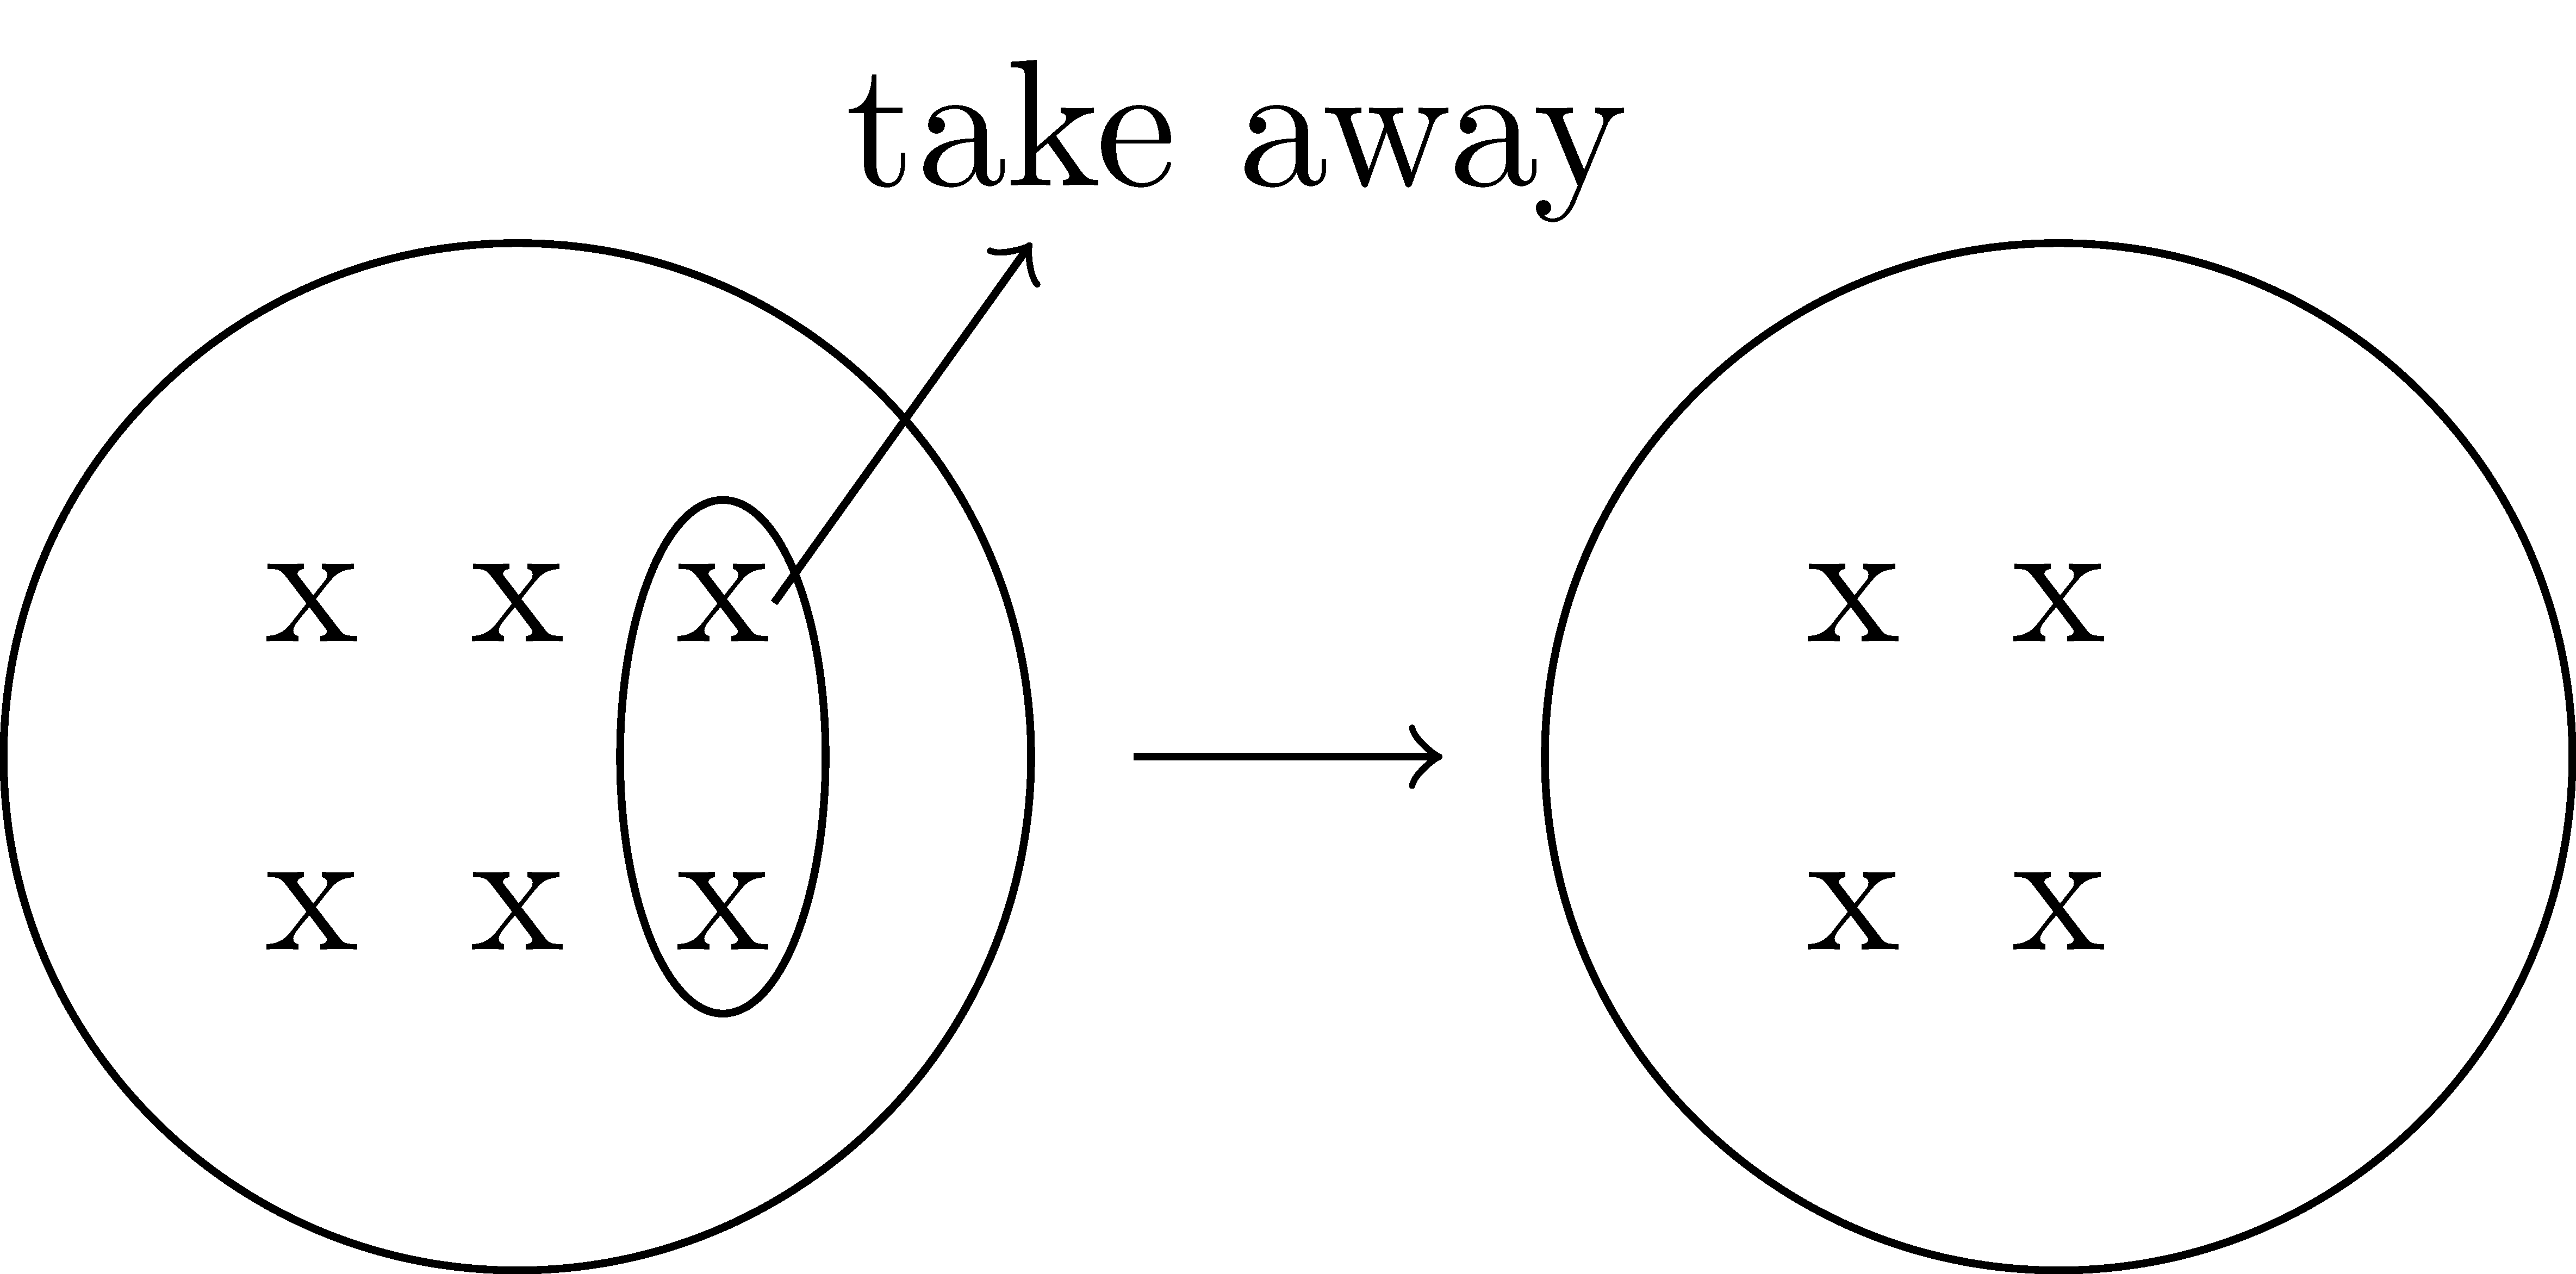
\includegraphics[width=0.3\linewidth]{tikz/subtraction-model-sets} 

}

\end{figure}

To model \(a-b\) using the number line and the take-away model, we find \(a\) on the number line and then move back \(b\) units. The place where you land is the resulting difference.

\begin{figure}

{\centering 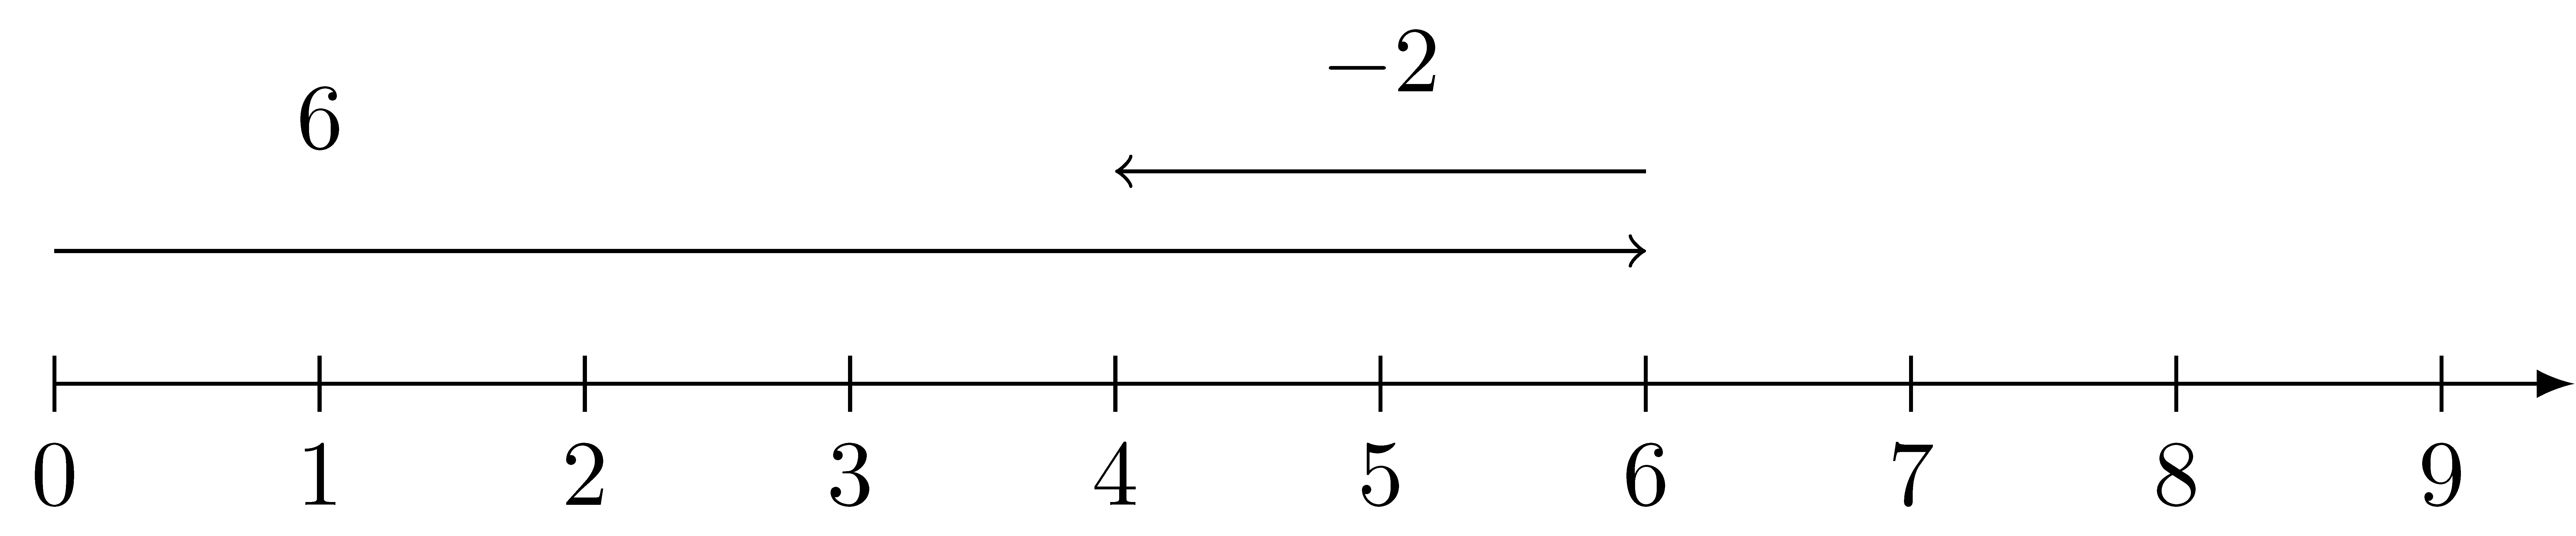
\includegraphics[width=0.7\linewidth]{tikz/subtraction-model-numberline} 

}

\end{figure}

Once we have introduced the integer number system, we extend the number line and think of \(a-b\) as \(a+(-b)\) where \(-b\) is viewed as a vector of length \(|b|\) pointed in the negative direction.

\begin{figure}

{\centering 
\includegraphics[width=0.8\linewidth]{tikz/subtraction-model-numberline2} 

}

\end{figure}

\begin{quote}
\hypertarget{related-content-standards-7}{%
\subsubsection*{Related Content Standards}\label{related-content-standards-7}}
\addcontentsline{toc}{subsubsection}{Related Content Standards}

\begin{itemize}
\tightlist
\item
  (6.NS.6) Understand a rational number as a point on the number line. Extend number line diagrams and coordinate axes familiar from previous grades to represent points on the line and in the plane with negative number coordinates.

  \begin{enumerate}
  \def\labelenumi{\alph{enumi}.}
  \tightlist
  \item
    Recognize opposite signs of numbers as indicating locations on opposite sides of \(0\) on the number line; recognize that the opposite of the opposite of a number is the number itself, e.g., \(-(-3) = 3\), and that \(0\) is its own opposite.
  \end{enumerate}
\end{itemize}
\end{quote}

\hypertarget{missing-addend-approach.}{%
\subsubsection*{Missing Addend Approach.}\label{missing-addend-approach.}}
\addcontentsline{toc}{subsubsection}{Missing Addend Approach.}

The missing addend approach interpretation of subtraction is an explicit model of subtraction as the inverse operation of addition, while converting the computationally more nuanced subtraction problem into an addition problem where the number facts and such are easier. In particular, in the missing addend approach, the subtraction expression \(a-b\) is assumed to equal some unknown (so \(a-b=?\)), which we can rewrite as \(b+?=a\).

Using the set model and the missing addend approach, we take the statement \(b+?=a\) to mean that we know that we want a set to contain \(a\) elements and we have \(b\). We must determine how many additional elements we need in order to bring the total number of things in our set up to \(a\).

\begin{figure}

{\centering 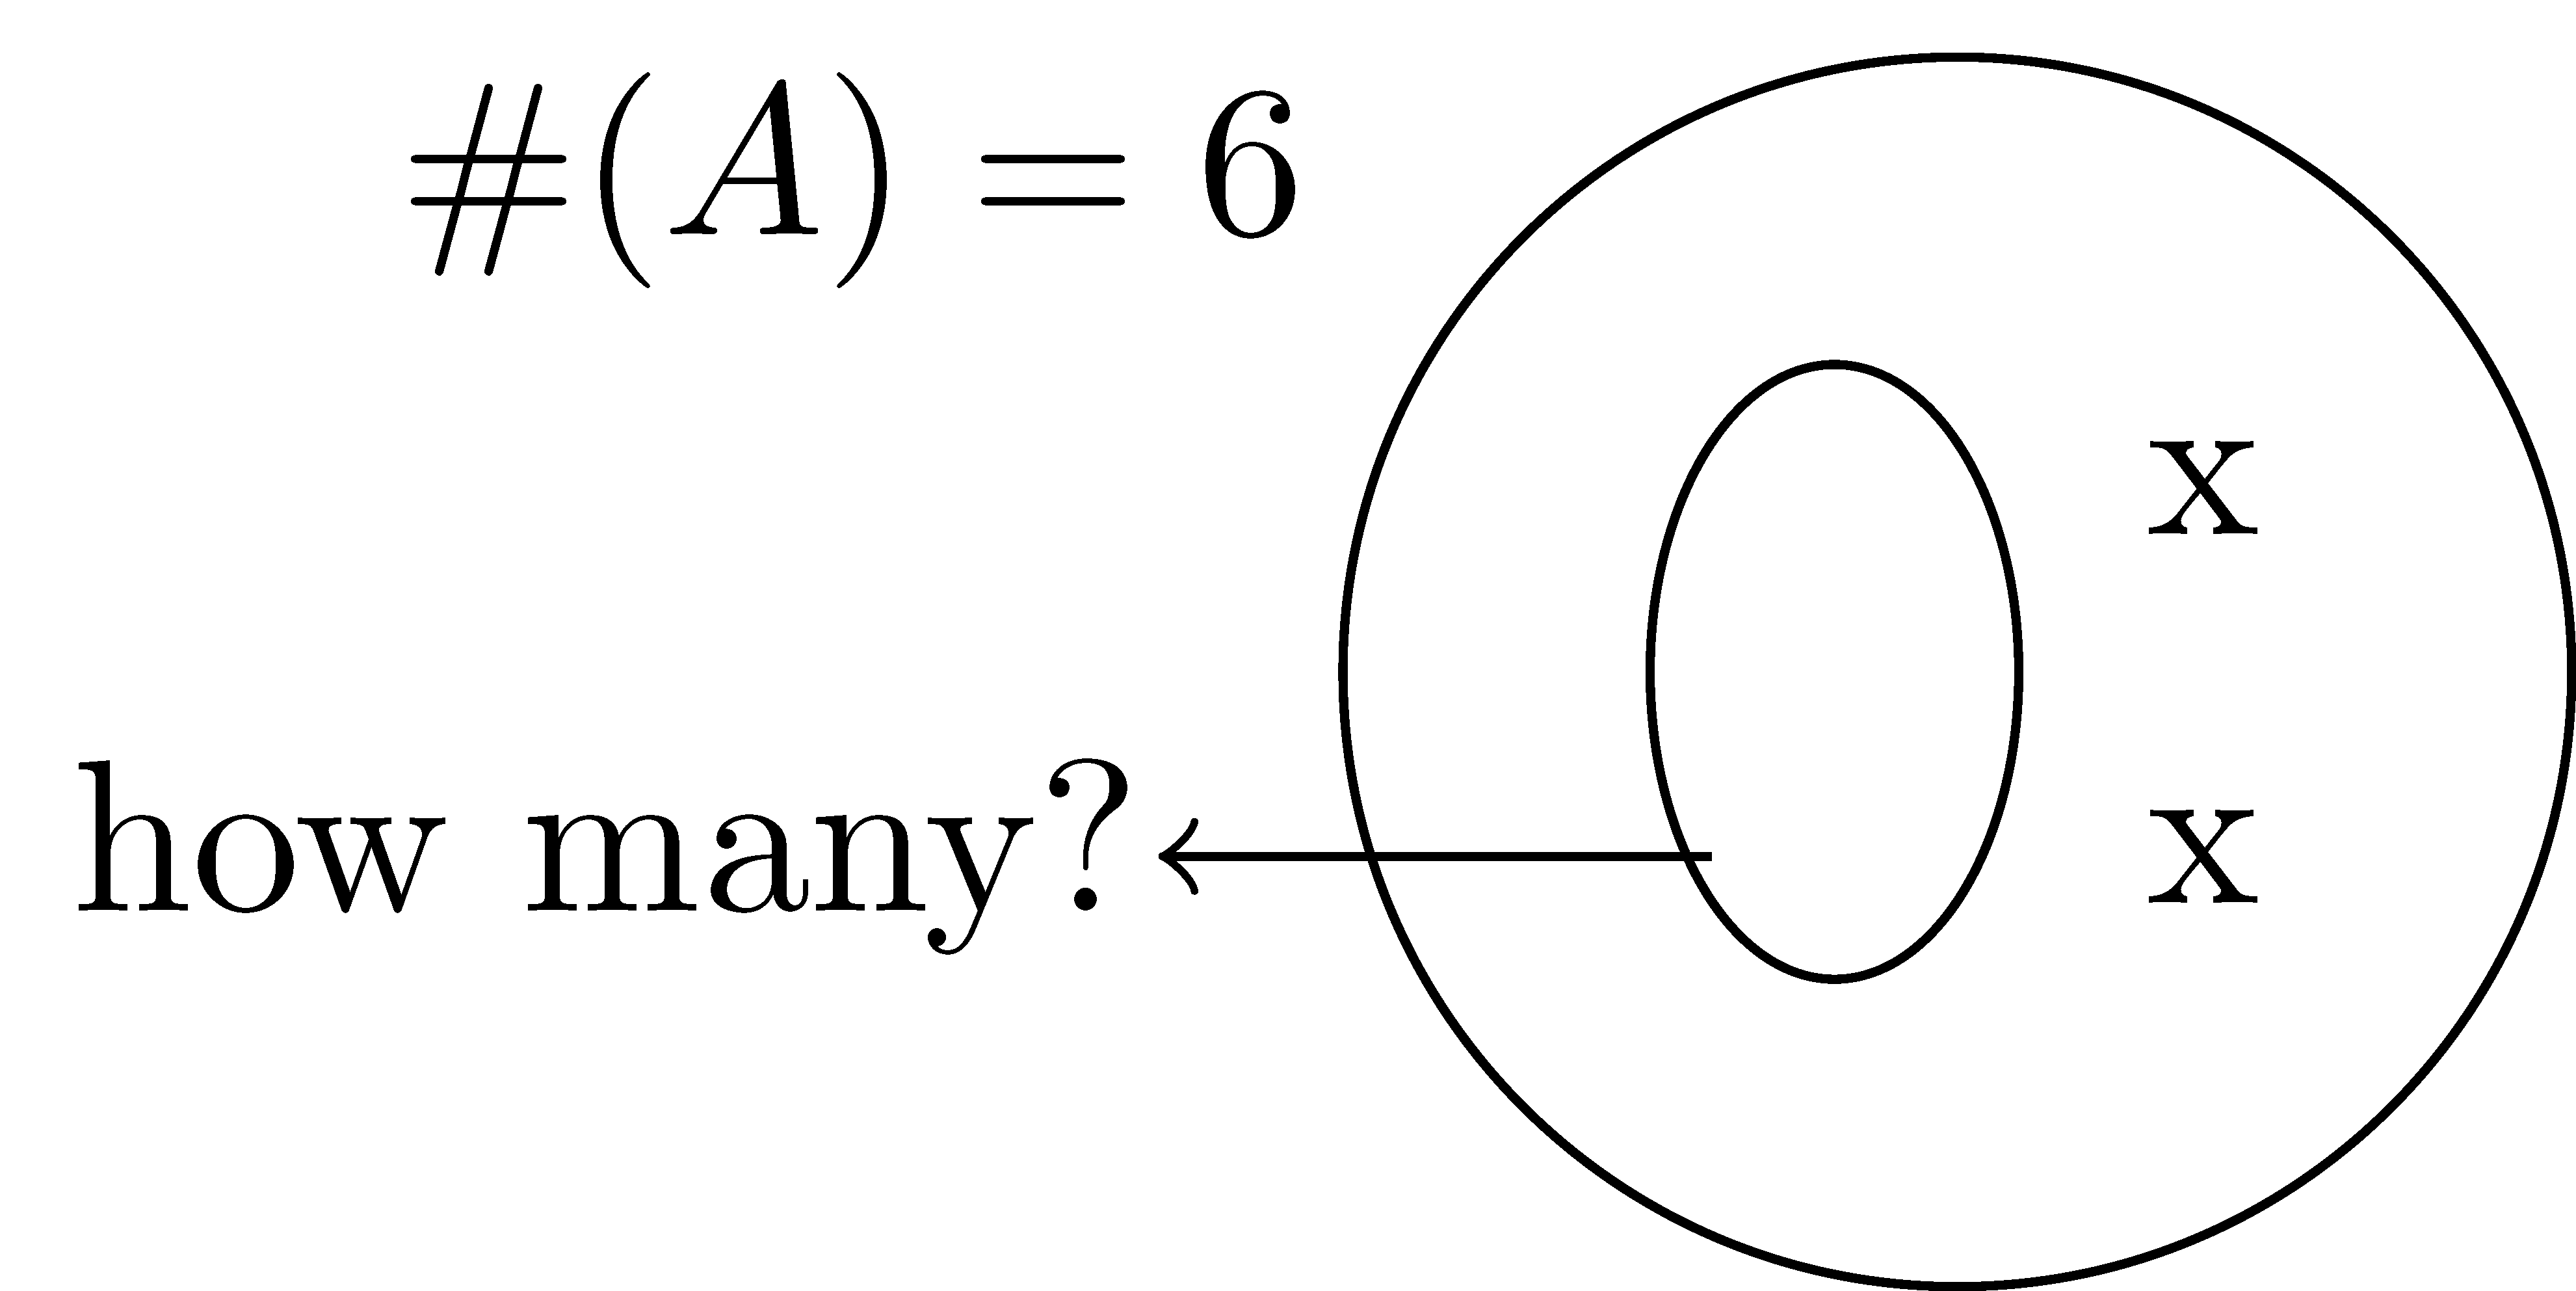
\includegraphics[width=0.4\linewidth]{tikz/subtraction-model-missingaddend-set} 

}

\end{figure}

Using the number line, we reconceptualize \(a-b=?\) As \(b+?=a\) which means we start at \(b\) on the number line and then find \(a\). We then ask, how much do I have to move (and in what direction) from \(b\) to get to \(a\)?. The answer to this question is the answer to the original subtraction problem. This process when formalized into an algorithm that counts up by place value is called \textbf{counting up}.

\begin{figure}

{\centering 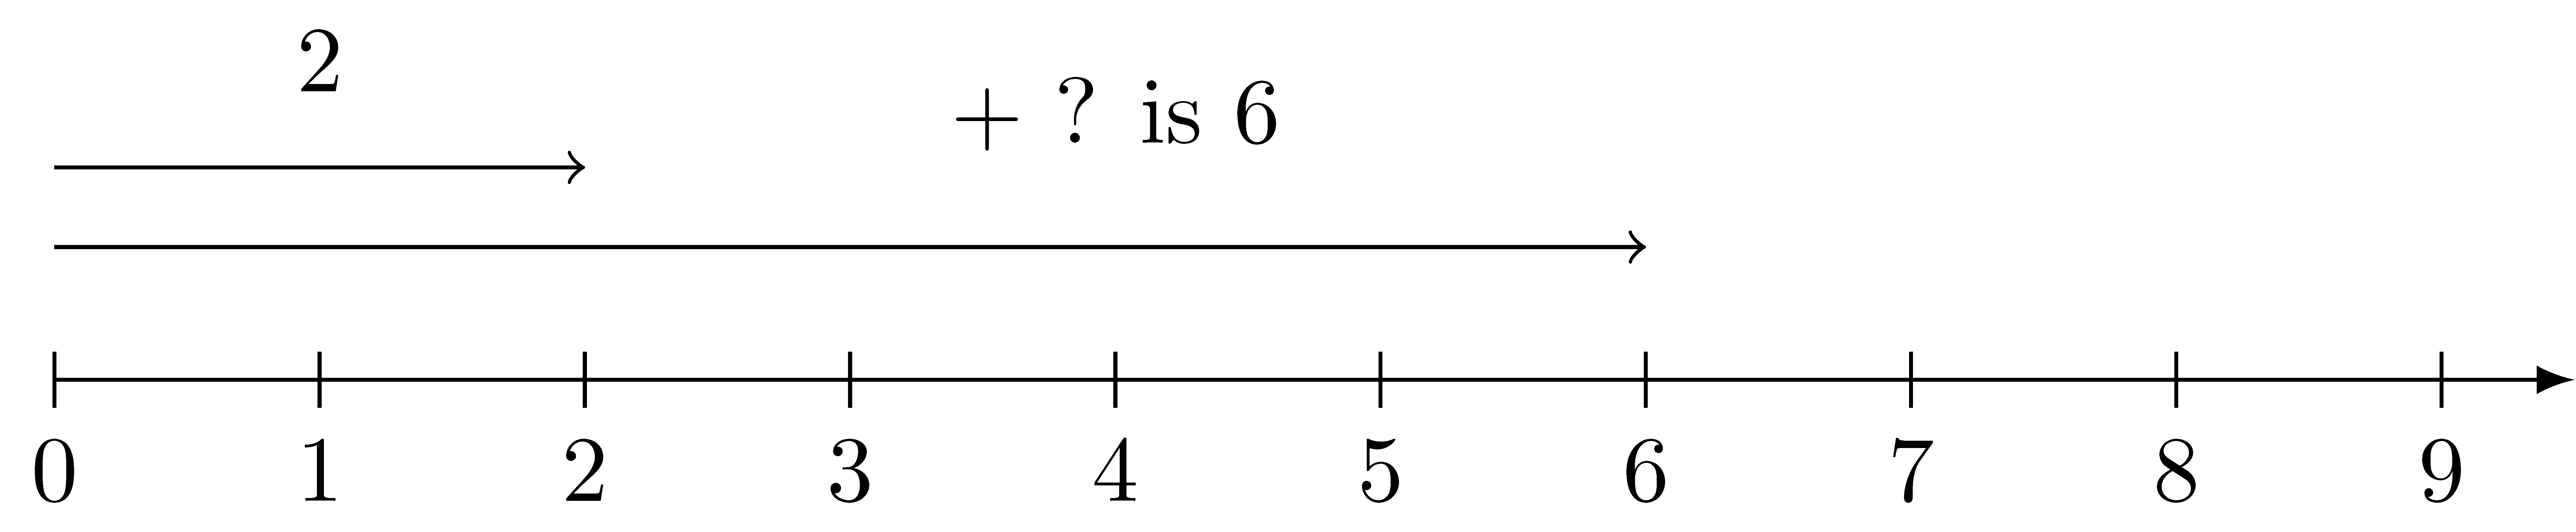
\includegraphics[width=0.8\linewidth]{tikz/subtraction-model-missingaddend-numberline} 

}

\end{figure}

Note that in none of the conceptual work of this section have we used the language of larger number and smaller number, instead focusing on the expression of the difference, \(a-b\). Early instruction in subtraction only presents cases of subtraction problems \(a-b\) when \(a\geq b\) and both are natural numbers. As a result of this presentation bias, students sometimes develop the impression that the results of subtraction will always be smaller than the original number. They may also believe that subtraction when \(a<b\) cannot be done. The conceptual work we have developed in this section for the models of subtraction works for most sets of numbers students encounter in the K-12 mathematics curriculum.

As with addition, we have a standard subtraction algorithm. For example, consider the subtraction problem \(423-368\). A well-trained student asked to do this problem without a calculator will produce work that looks something like the following:

\begin{figure}

{\centering 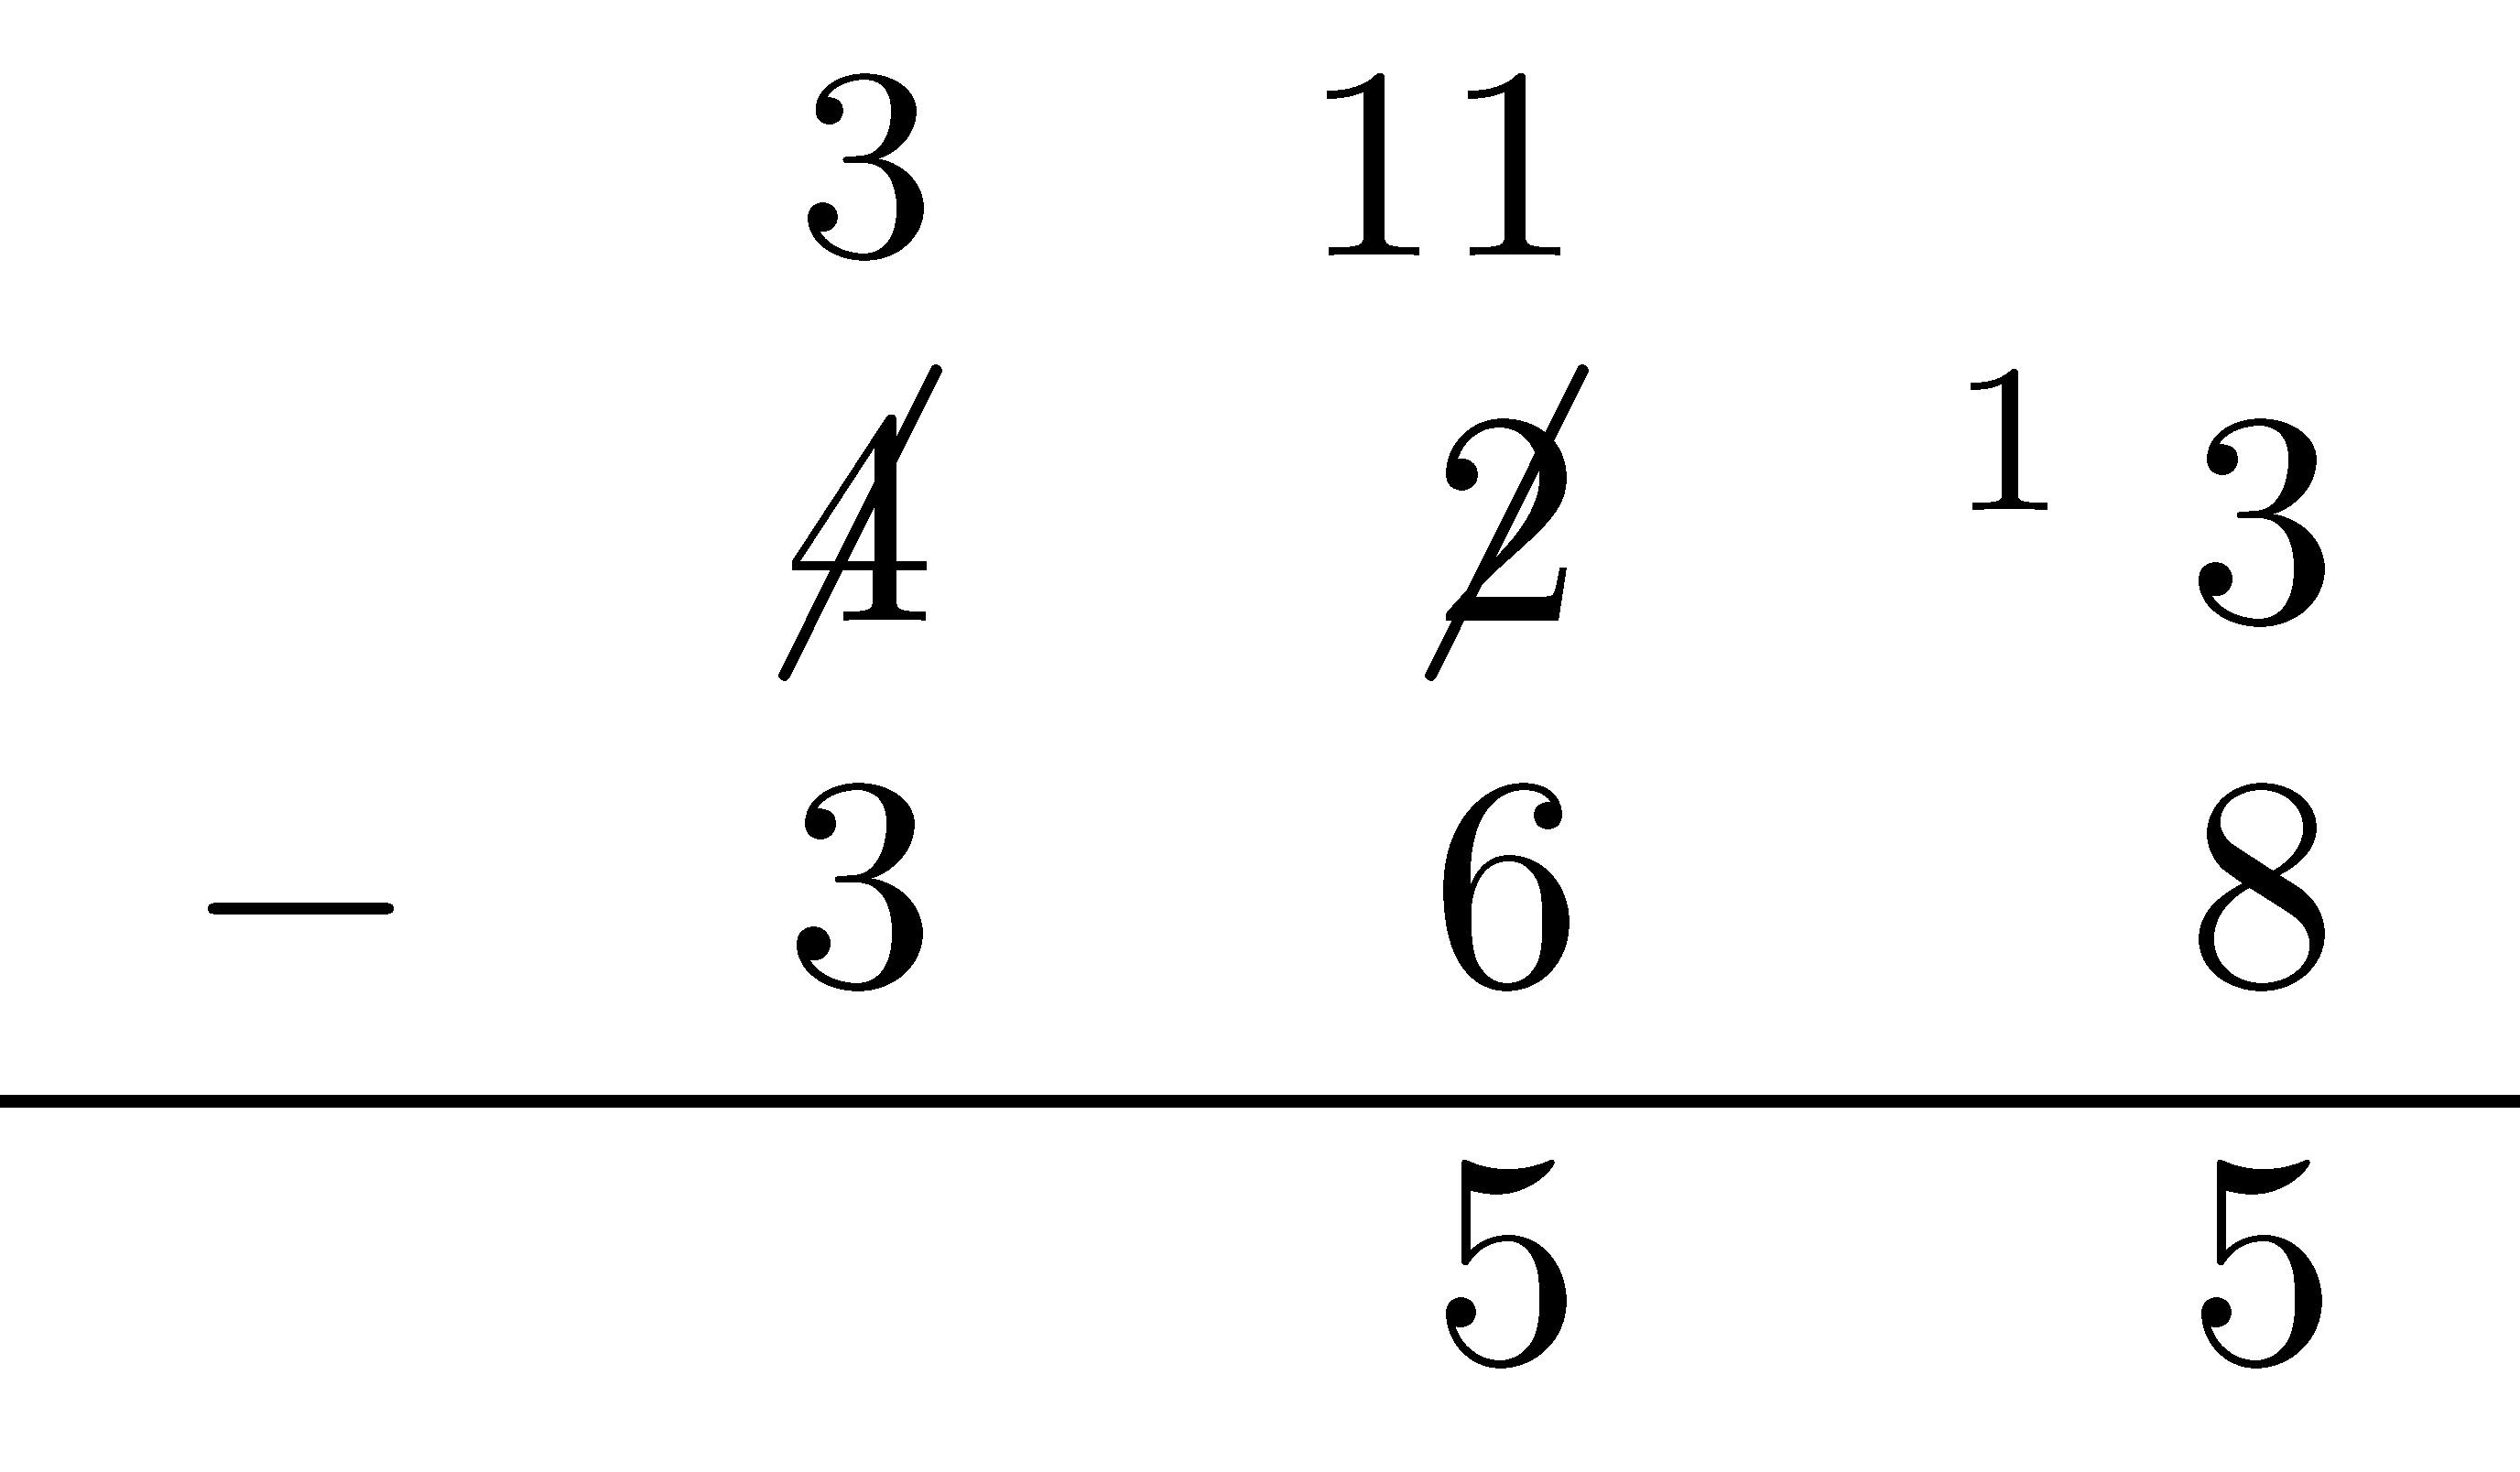
\includegraphics[width=0.3\linewidth]{tikz/subtraction-model-algorithm} 

}

\end{figure}

As with addition, the traditional subtraction algorithm uses regrouping strategies and the properties of place value to allow for quick calculation in a small amount of space. (You may have learned the regrouping strategy under the name ``borrowing'' but, as with addition, this name is no longer used for similar reasons.)

We next provide several alternative algorithms for subtraction designed to help develop conceptual understanding of the subtraction algorithm.

\hypertarget{equal-addition.}{%
\subsubsection*{Equal Addition.}\label{equal-addition.}}
\addcontentsline{toc}{subsubsection}{Equal Addition.}

The equal addition algorithm repeatedly adds zero to the problem in a way that makes the subtraction easier to compute. The goal is to write an equivalent problem that has at least one zero place value.

\begin{align*}
423-368 &= 423-368 + (2-2) = 425-370 \\
  &= (425-370) + (30-30) = 455-400 \\
  &= 55
\end{align*}

\hypertarget{partial-differences.}{%
\subsubsection*{Partial Differences.}\label{partial-differences.}}
\addcontentsline{toc}{subsubsection}{Partial Differences.}

Another method of subtraction is to subtract from left to right with partial differences. In this case, we subtract the smaller digit from the larger digit, keeping track of positive or negative.

\begin{figure}

{\centering 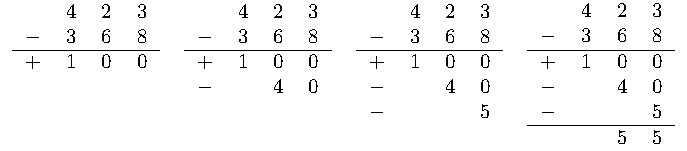
\includegraphics[width=0.8\linewidth]{tikz/subtraction-model-partial-differences} 

}

\end{figure}

In the section on subtraction, we commented that when students first learn subtraction in the natural numbers, they are usually only given examples of the form \(a-b\) where \(b\leq a\). Part of the reason for only having students work on these types of problems is that children are not born knowing about negative numbers. The only place we ``see'' negative numbers in the real world is when humans have imposed a scale on something, such as temperature. However, this is not a true physical representation, since we have simply imposed a scale on a naturally occurring thing, where for one reason or another, we want to have a zero reference point.

To allow us to find answers to subtraction problems where \(a<b\), we expand our number system to the integers.
You may have noticed that we use ``\(-\)'' in the above paragraph to mean additive inverse of a positive number. In the paragraph before that we used the same symbol to mean subtraction. In reality, these are fairly different concepts. Subtraction is an operation. Additive inverse is a relation. Long-time students of mathematics know that these interpretations are related and will move between them fairly seamlessly, but they are not the same thing.

\hypertarget{multiplication-models-and-algorithms}{%
\subsection{Multiplication Models and Algorithms}\label{multiplication-models-and-algorithms}}

\hypertarget{repeated-addition.}{%
\subsubsection*{Repeated Addition.}\label{repeated-addition.}}
\addcontentsline{toc}{subsubsection}{Repeated Addition.}

Most commonly, multiplication is described as \textbf{repeated addition}. For example, the product \(2\times 4\) can be understood as adding \(2\) four times (\(2+2+2+2\)), while the product \(4\times 2\) can be understood as adding \(4\) two times (\(4+4\)). While conceptually, this link between addition and multiplication is important, it quickly loses efficiency in practical applications (e.g., it would be cumbersome but possible to multiply \(23\times 345\) using repeated addition). that said, it is not uncommon to see secondary students apply this approach to multiplication problems.

\hypertarget{rectangular-array.}{%
\subsubsection*{Rectangular Array.}\label{rectangular-array.}}
\addcontentsline{toc}{subsubsection}{Rectangular Array.}

Another way to represent multiplication is through a \textbf{rectangular array}. One way to think about this is counting the number of chairs in \(a\) rows and \(b\) columns. Such arrays are discrete sets. We can see below how one can use two arrays to represent \(3\times 5\) and \(5 \times 3\).

\begin{figure}

{\centering 
\includegraphics[width=0.5\linewidth]{tikz/arrays} 

}

\end{figure}

We can see that the two arrays are related to each other by a rotation. In other words, the order of multiplication is simply a different perspective on the same array.

\hypertarget{area-model.}{%
\subsubsection*{Area Model.}\label{area-model.}}
\addcontentsline{toc}{subsubsection}{Area Model.}

While arrays work well for representing multiplication of natural numbers, they do not work well for integers, rational numbers, or real numbers. So we generalize the array model to an \textbf{area model}. If we change the dots in the array to blocks of 1 square unit measure, the above arrays become rectangles with square tiles helping students see the connection between the area of a rectangle and multiplication.

\begin{figure}

{\centering 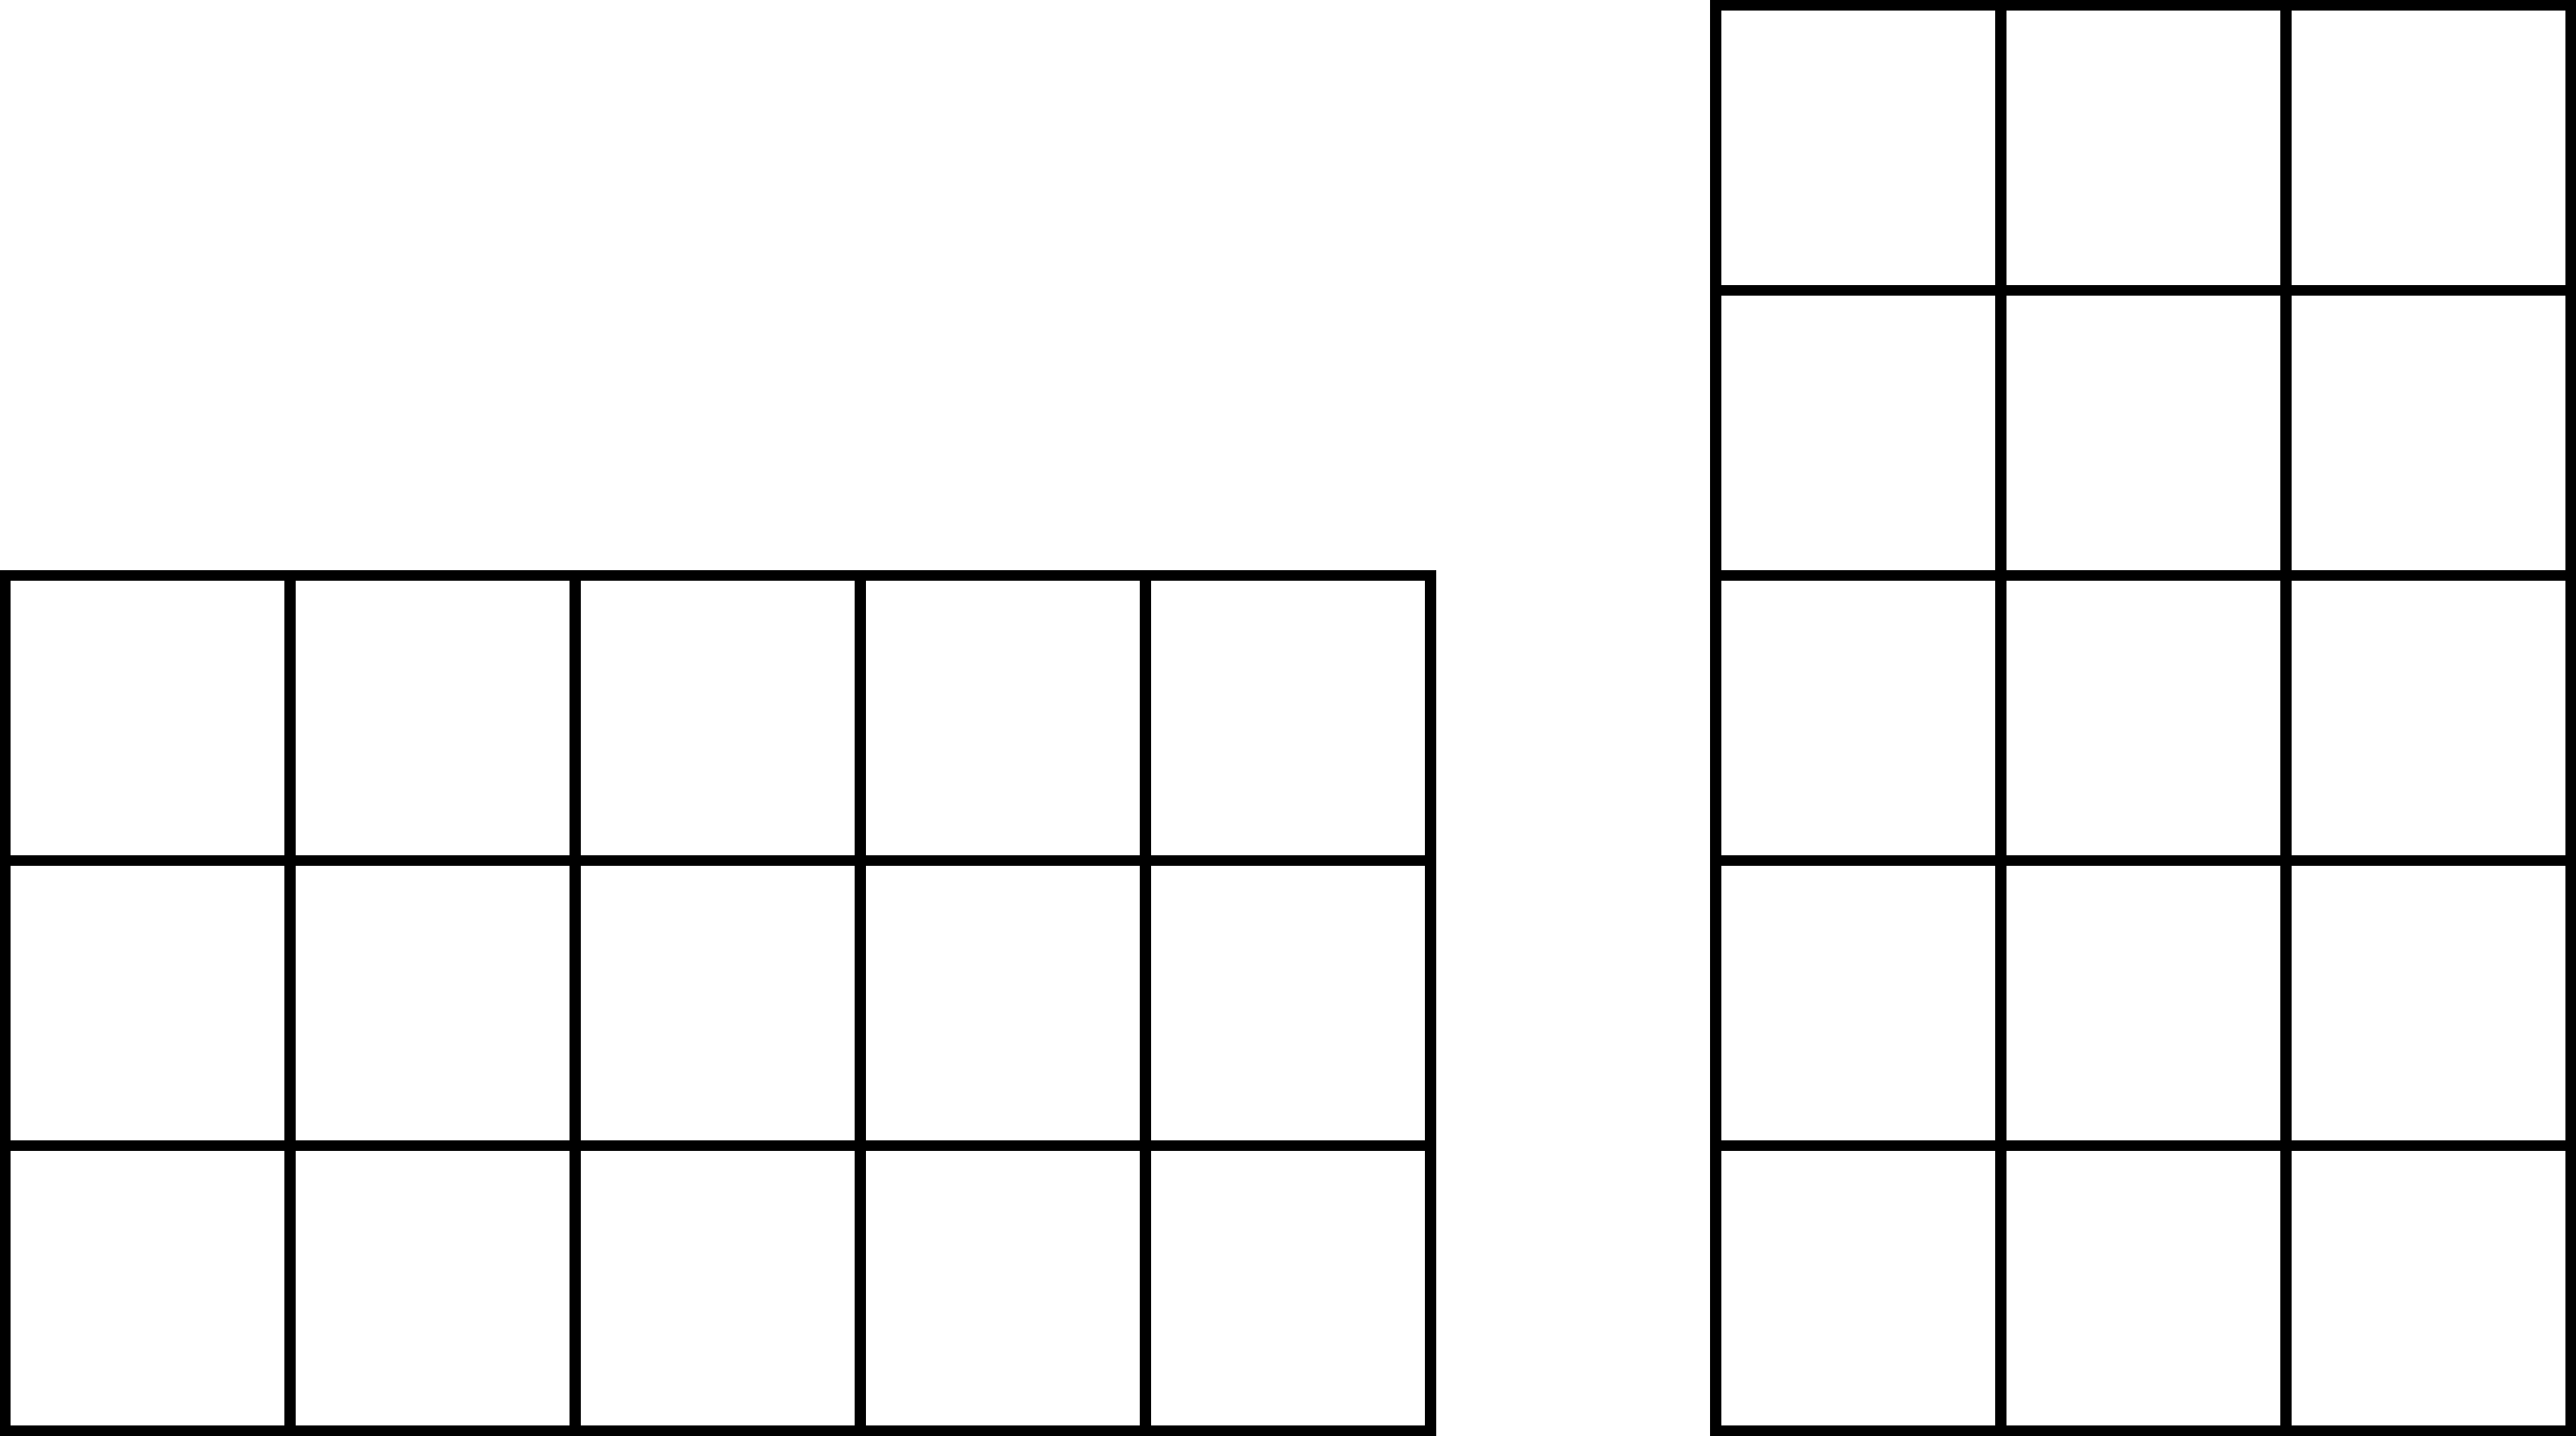
\includegraphics[width=0.5\linewidth]{tikz/area-model-3by5} 

}

\end{figure}

This area model can then be generalized to help students multiply multi-digit natural numbers and the relationship to the distribution property.

\begin{figure}

{\centering 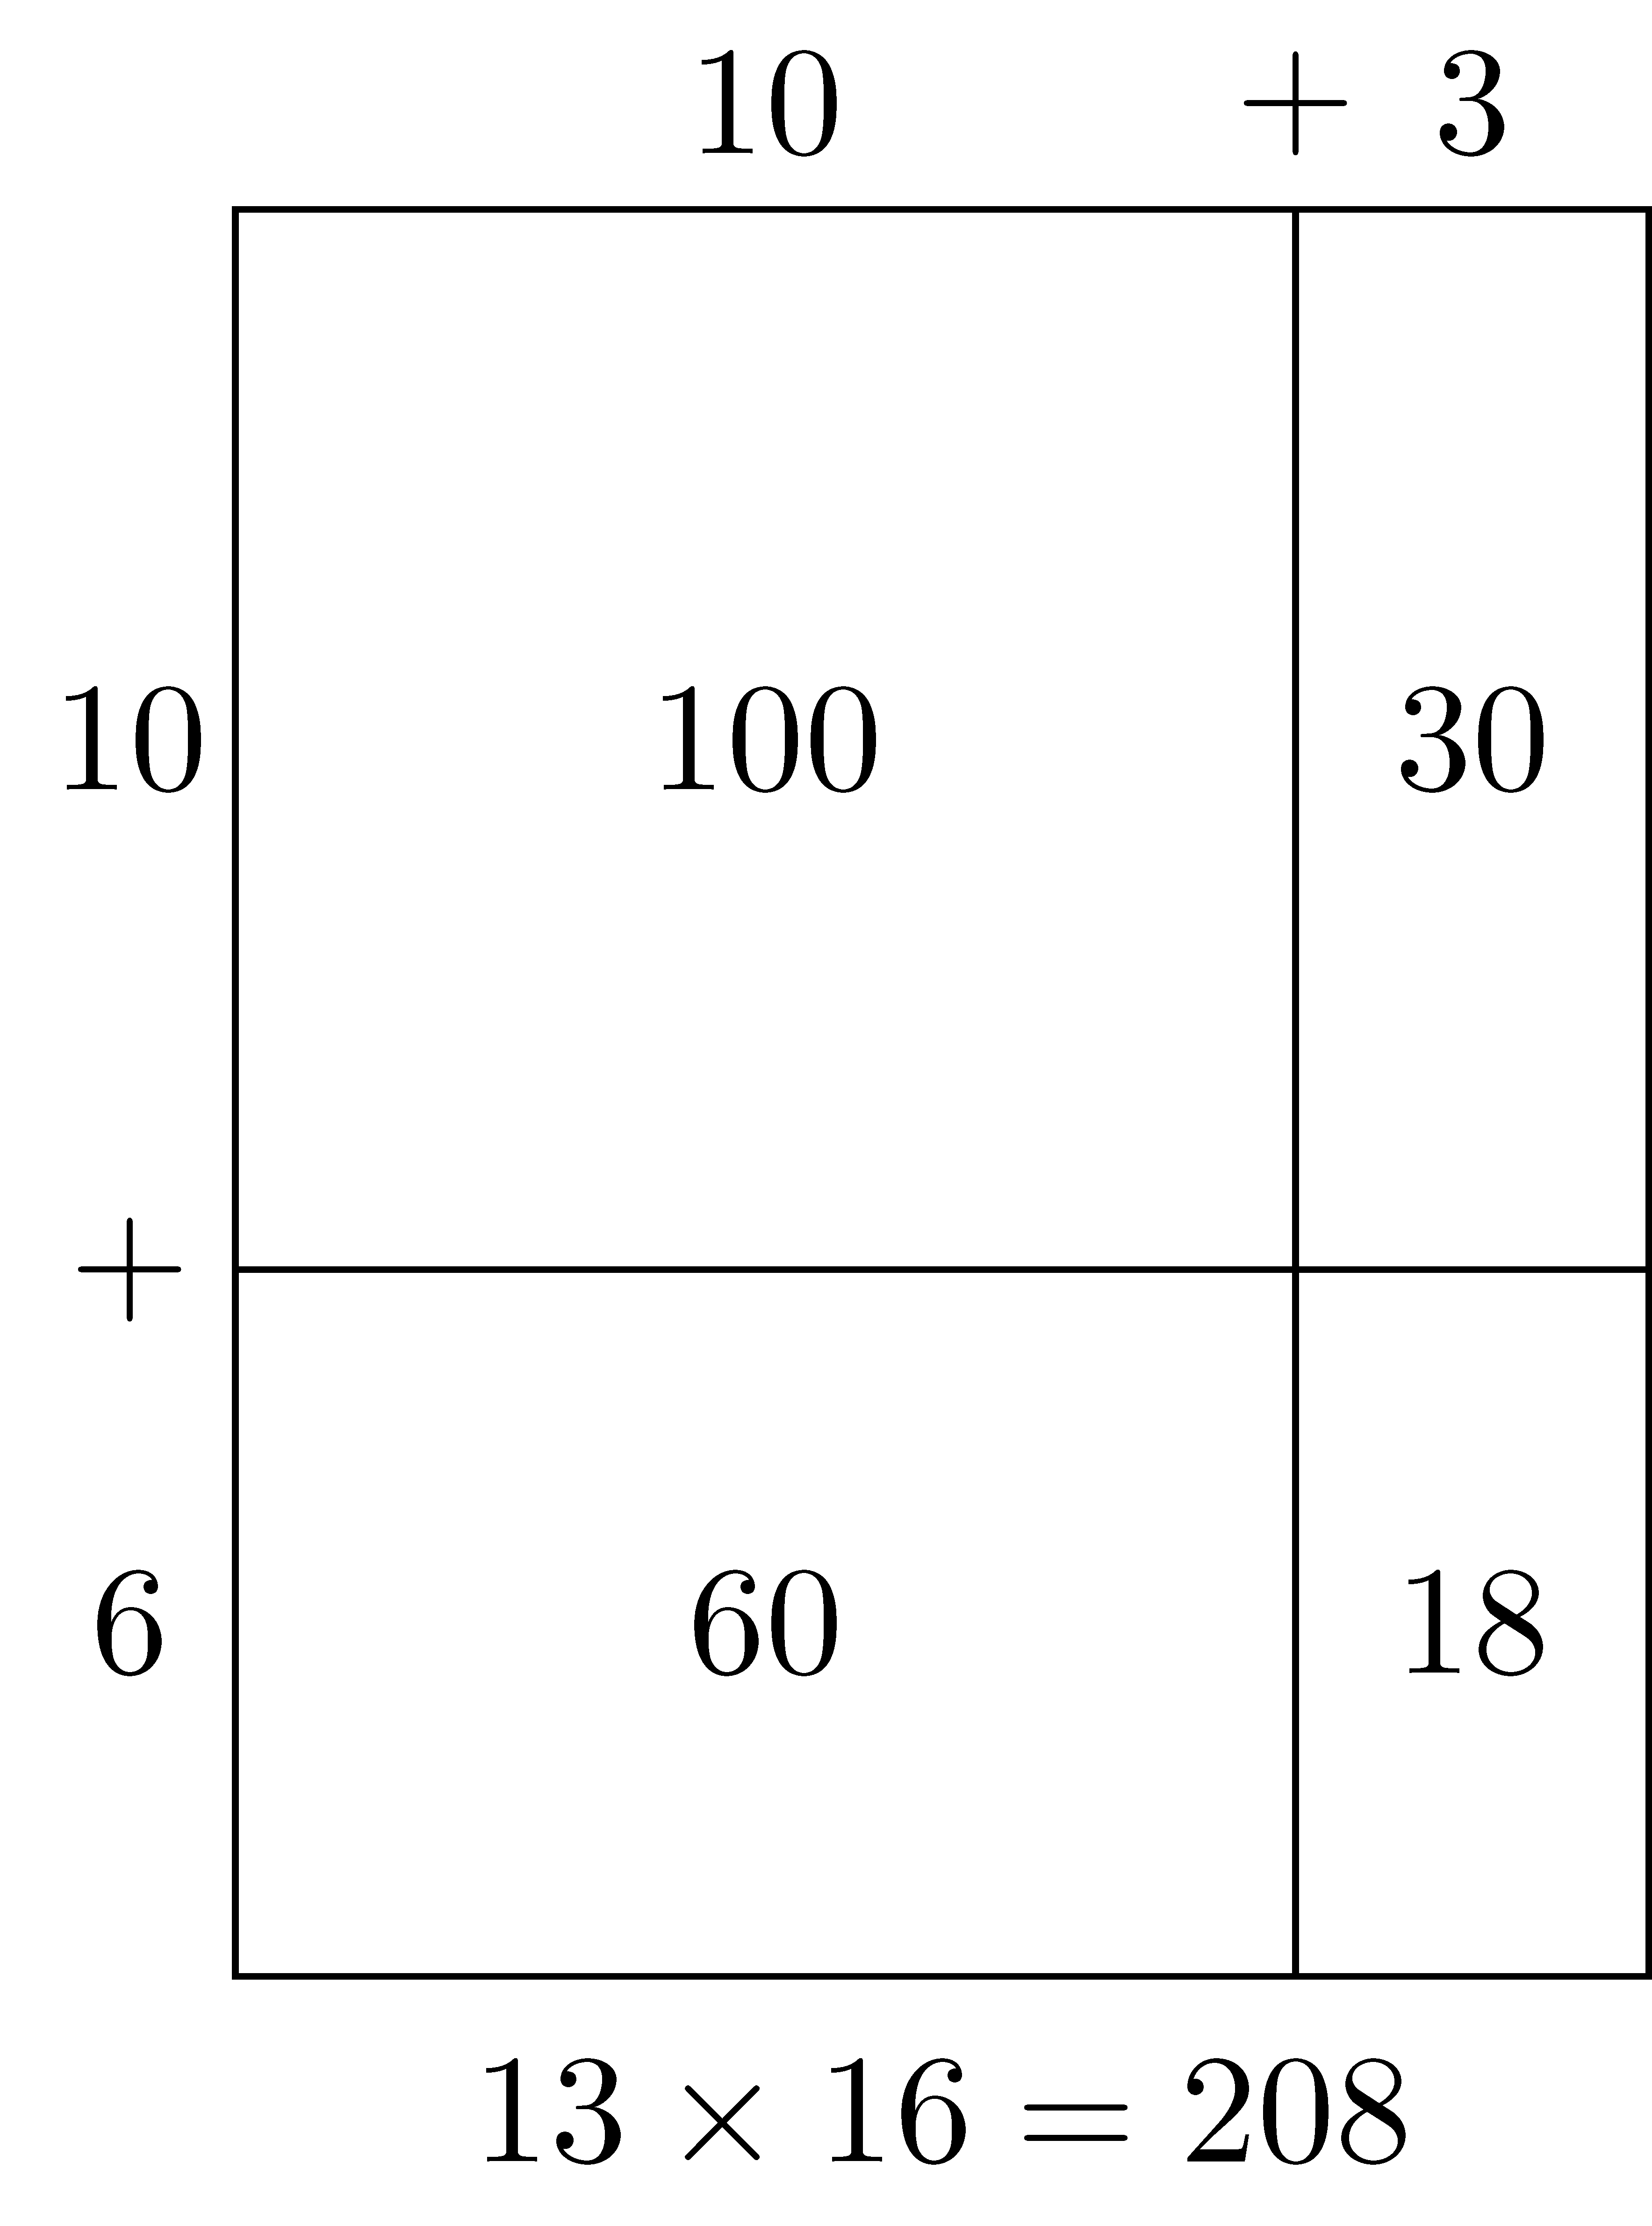
\includegraphics[width=0.4\linewidth]{tikz/area-model-13-16} 

}

\end{figure}

\hypertarget{lattice-multiplication.}{%
\subsubsection*{Lattice Multiplication.}\label{lattice-multiplication.}}
\addcontentsline{toc}{subsubsection}{Lattice Multiplication.}

The area model can become unwieldy with larger numbers. The lattice multiplication algorithm is a more abstract view of the area model by using a lattice to keep track of place values. Here we can see the progression of using a lattice model to multiply \(54 \times 68 = 3672\).

\begin{figure}

{\centering 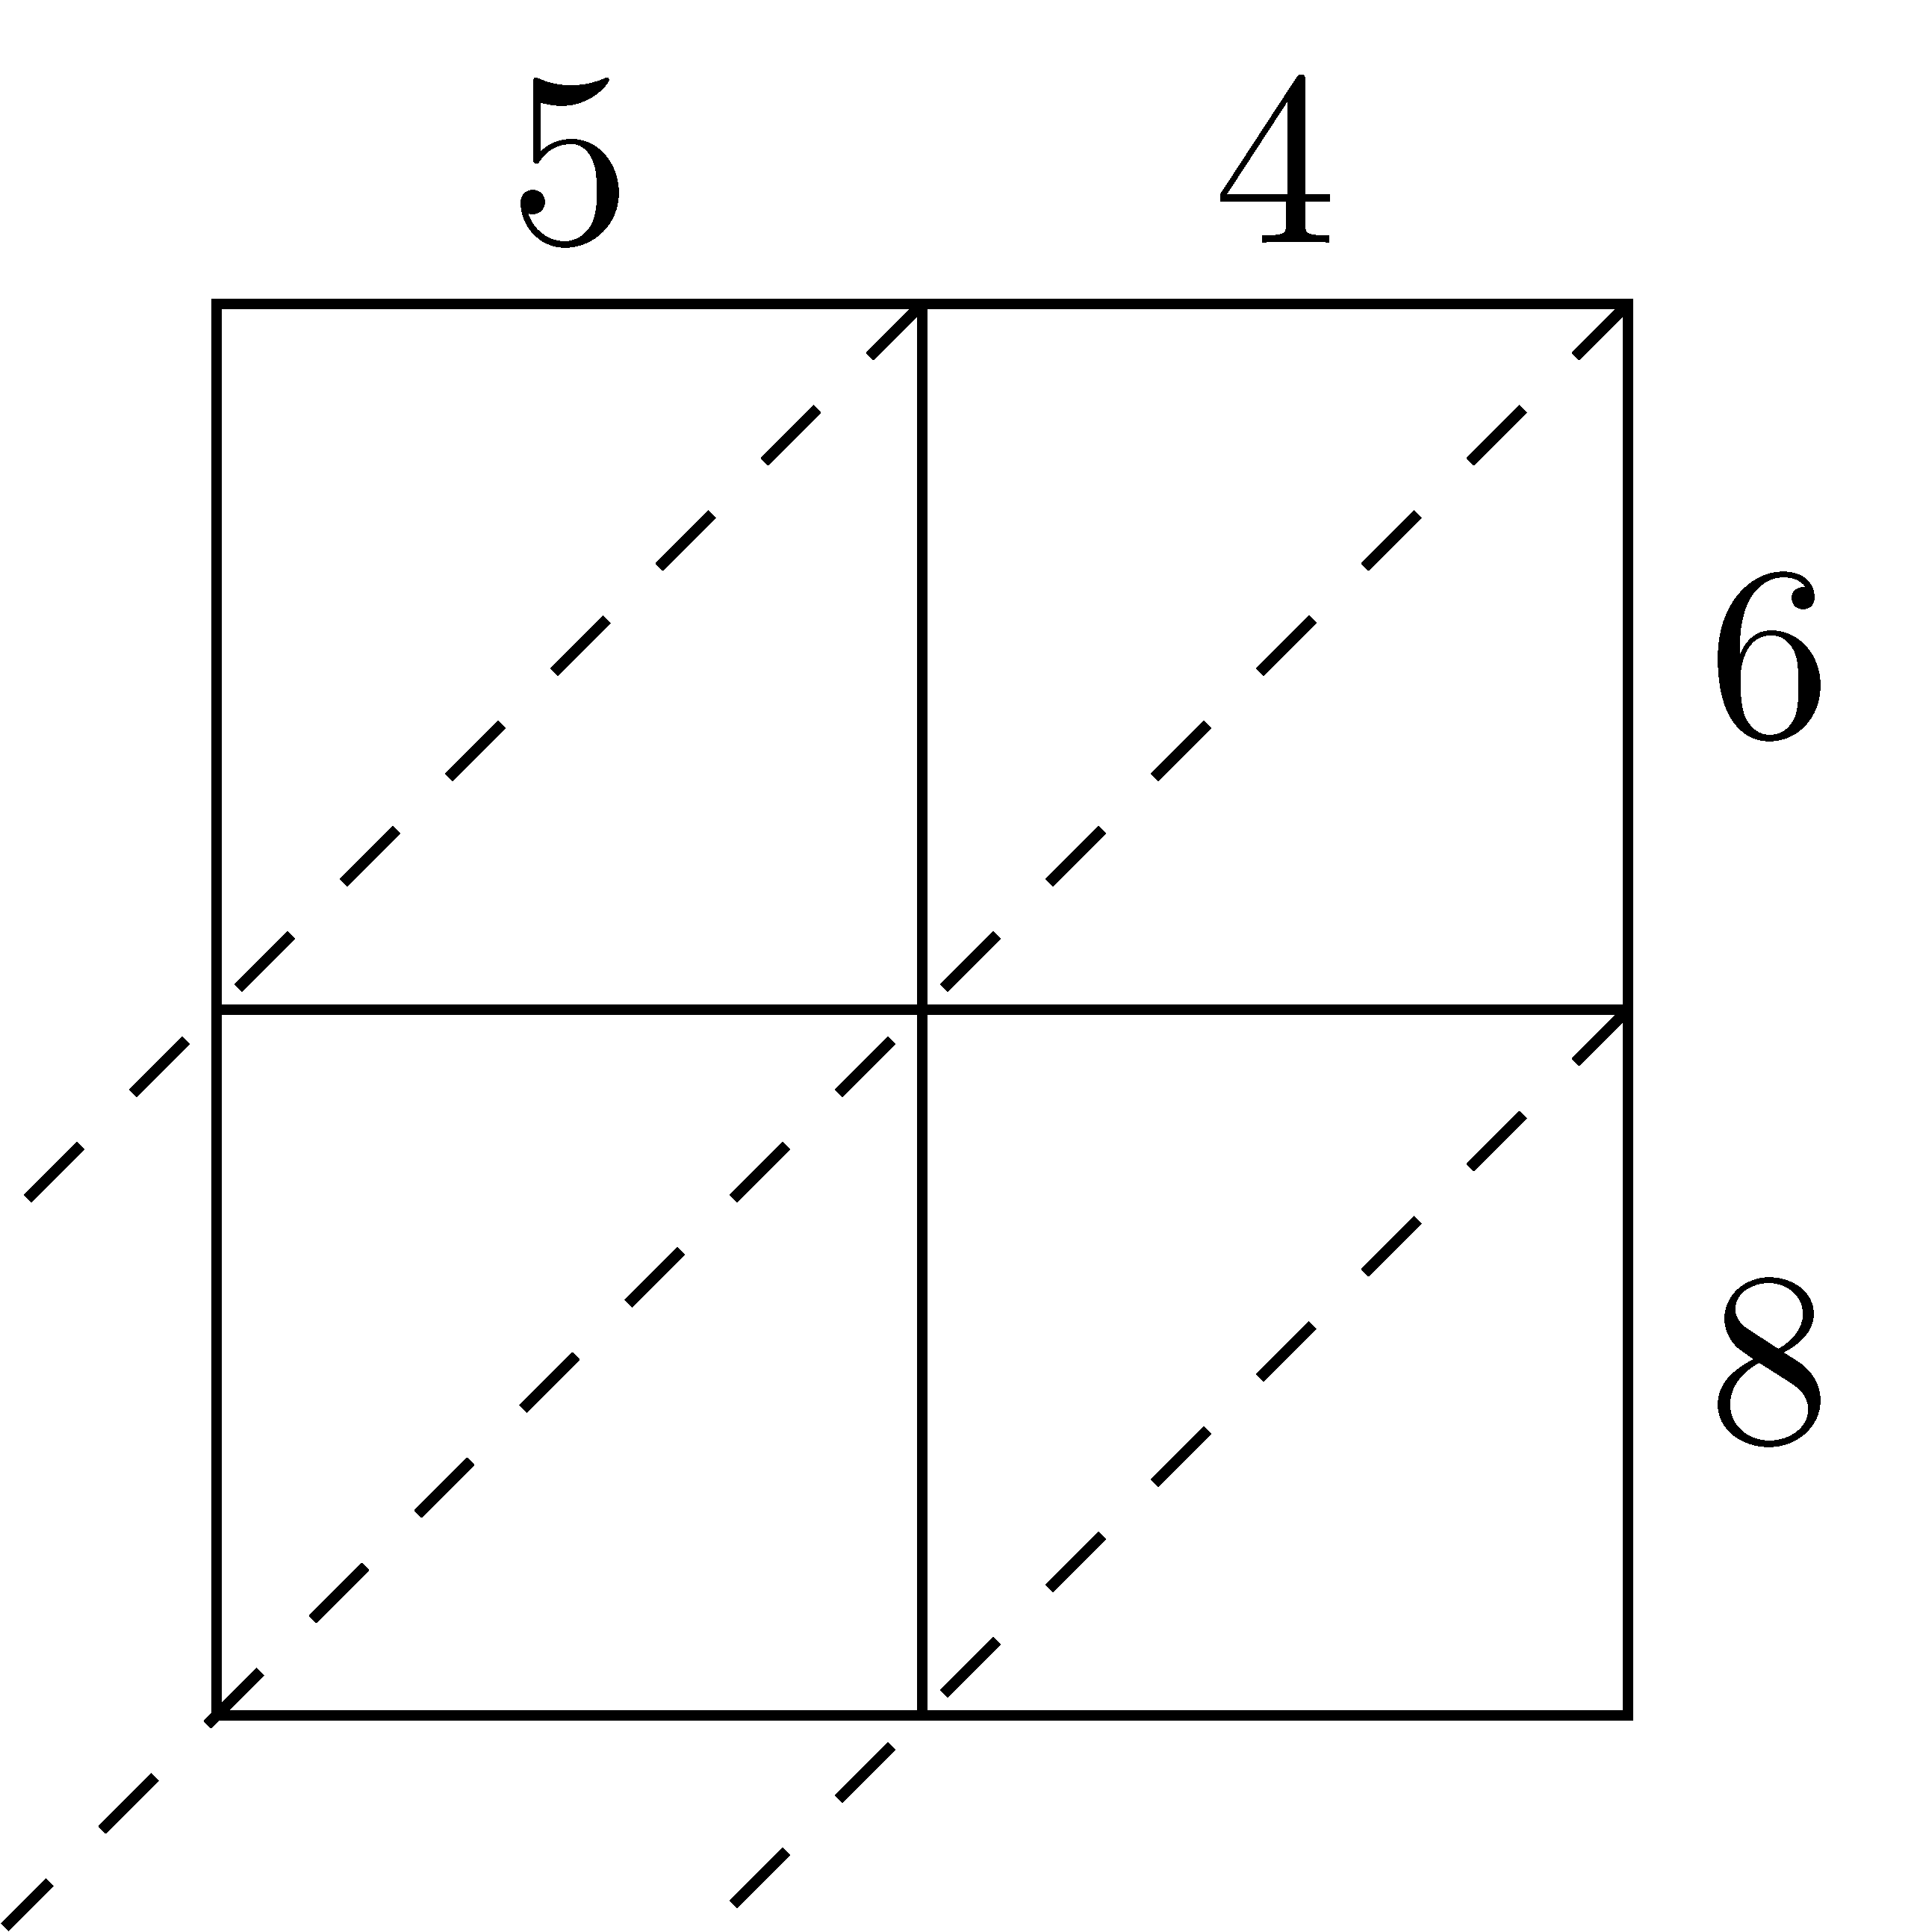
\includegraphics[width=0.5\linewidth]{tikz/lattice-multiplication-13-16-1} 

}

\end{figure}
\begin{figure}

{\centering 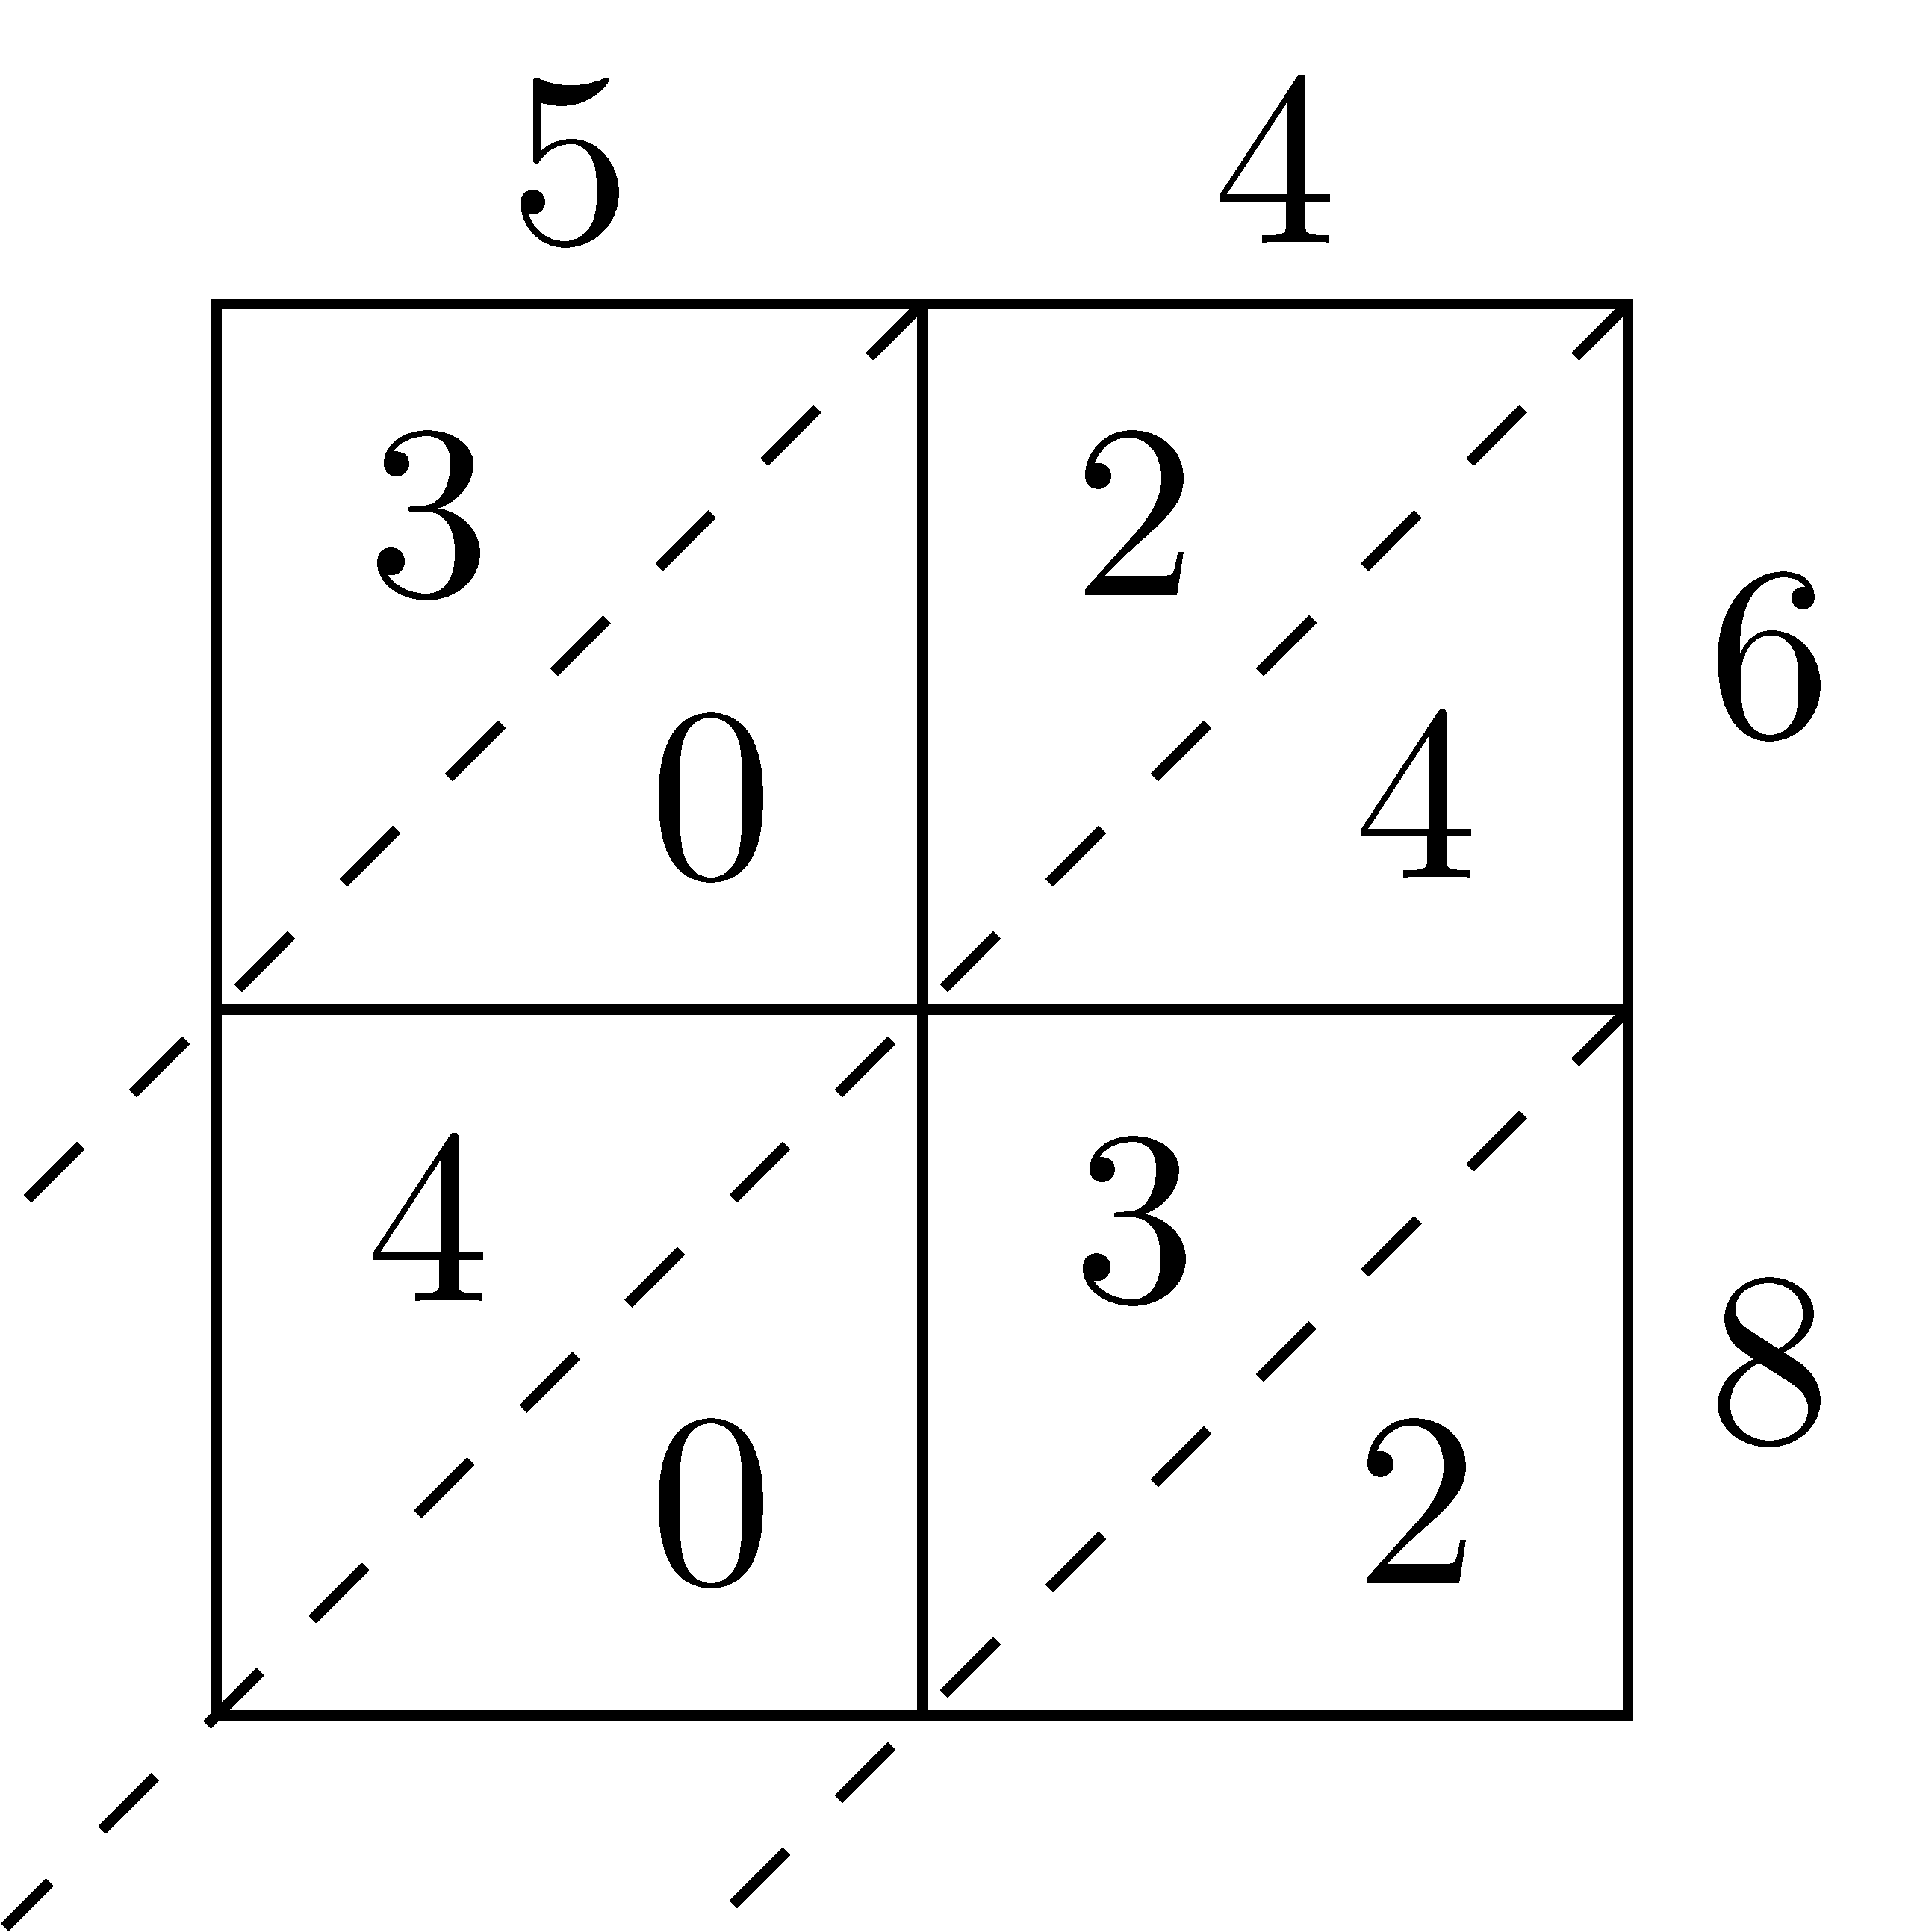
\includegraphics[width=0.5\linewidth]{tikz/lattice-multiplication-13-16-2} 

}

\end{figure}
\begin{figure}

{\centering 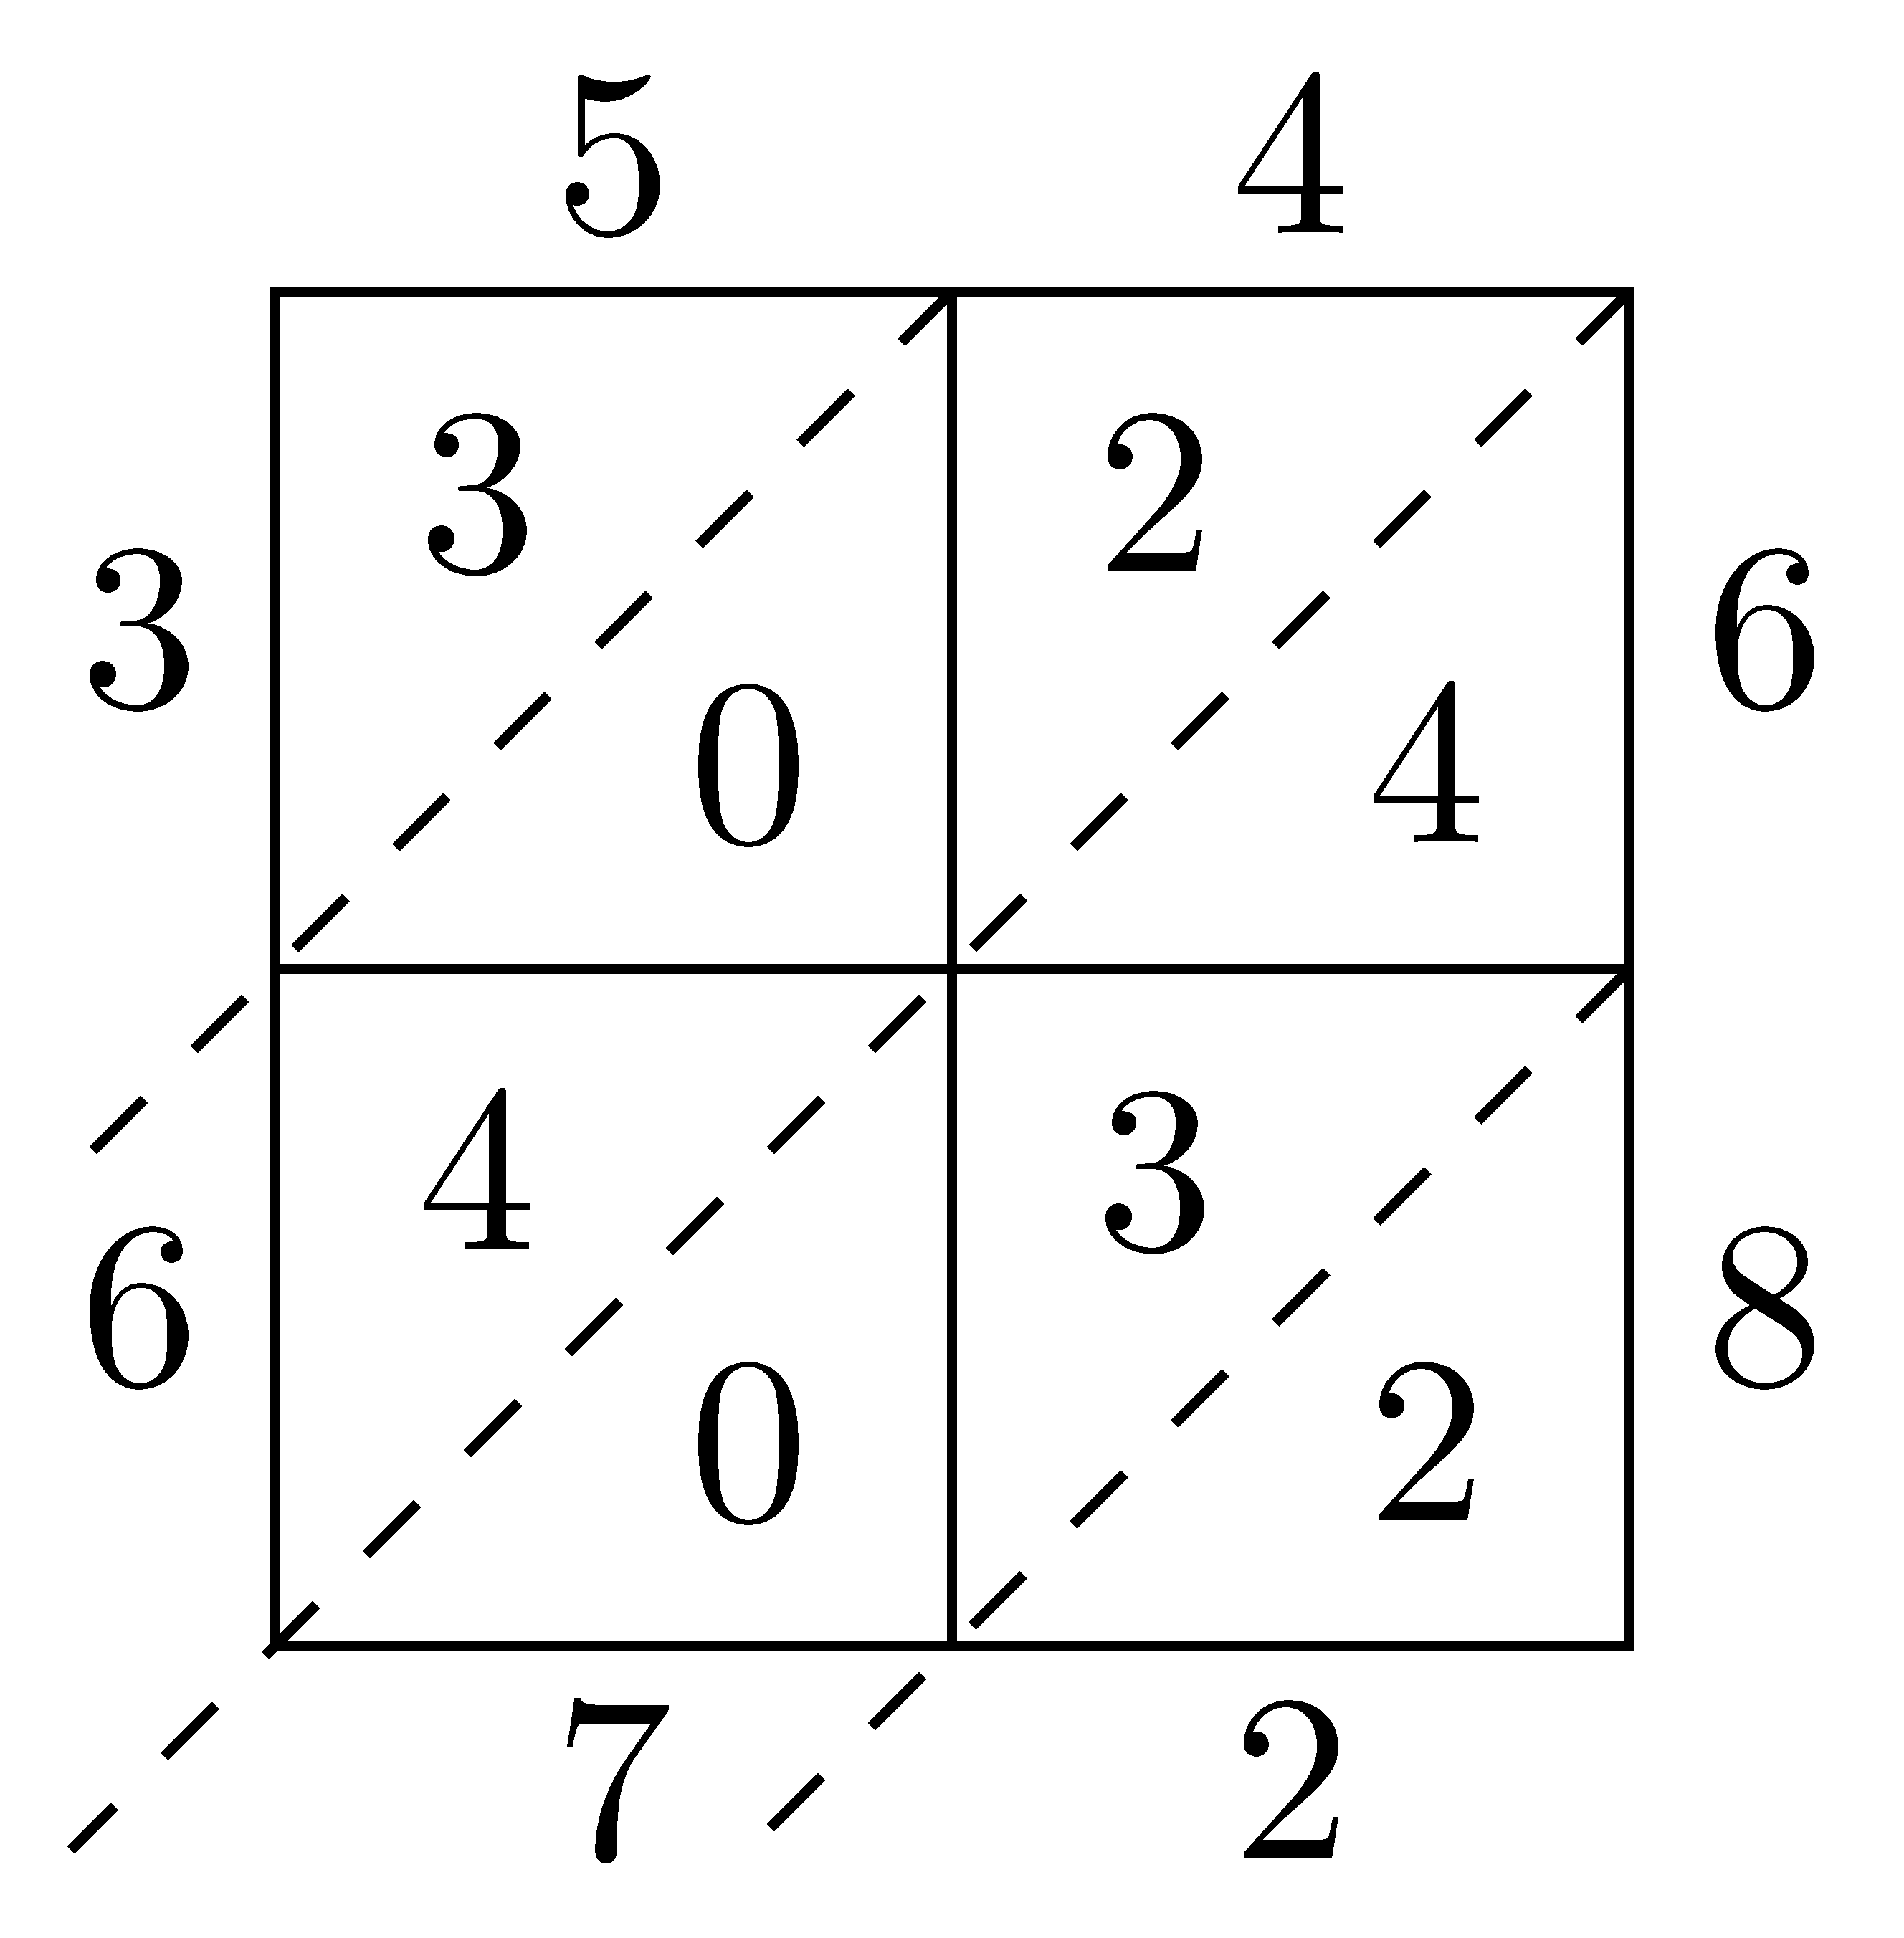
\includegraphics[width=0.5\linewidth]{tikz/lattice-multiplication-13-16-3} 

}

\end{figure}

After setting up the lattice with diagonals, we multiply all of the partial products and enter the product in the corresponding square with the one's digit in the bottom right and the ten's digit in the upper left. After all of the partial products are complete, we add along the diagonals in order to find the number of units of that place value. For some products, the sum along the diagonal is larger than \(9\) and so we have to regroup as is the case for \(1564 \times 63\).

\begin{figure}

{\centering \includegraphics[width=0.6\linewidth]{tikz/lattice-multiplication-large} 

}

\end{figure}

\hypertarget{partial-products.}{%
\subsubsection*{Partial Products.}\label{partial-products.}}
\addcontentsline{toc}{subsubsection}{Partial Products.}

We continue the progression of creating more abstract algorithms for multiplication by removing some of the explicit structure using the \textbf{partial products algorithm}.

\begin{figure}

{\centering \includegraphics[width=0.6\linewidth]{tikz/partial-products} 

}

\end{figure}

\hypertarget{standard-u.s.-multiplication-algorithm.}{%
\subsubsection*{Standard U.S. Multiplication Algorithm.}\label{standard-u.s.-multiplication-algorithm.}}
\addcontentsline{toc}{subsubsection}{Standard U.S. Multiplication Algorithm.}

If we continue down the path of more abstract algorithms we come to what is considered the standard algorithm for multiplication. In this algorithm we compress the information in the partial products algorithm into many fewer lines.

\begin{figure}

{\centering \includegraphics[width=0.6\linewidth]{tikz/multiplication-algorithm-standard} 

}

\end{figure}

However, with this reduction in the number of lines comes an increase in the number of things that one must keep track of implicitly.

\hypertarget{division-models-and-algorithms}{%
\subsection{Division Models and Algorithms}\label{division-models-and-algorithms}}

Division is the fourth major operation. Conceptually, the division problem \(a \div b\) can be viewed several ways: as repeated subtraction, as the inverse of multiplication, and as a partition. Regardless of the model, all three of these representations draw on the notion that when we divide \(a\) by \(b\) (\(a\div b\)) the division operation produces two unique numbers: the \textbf{quotient}, \(q\), and the \textbf{remainder}, \(r\), where \(0\leq r <b\). (We will go into this division algorithm more in-depth in Section \ref{sec:Integer-Ring}.) We call \(b\) the \textbf{divisor} and \(a\) the \textbf{dividend}. These four quantities are related by \(a=bq+r\).

\hypertarget{repeated-subtraction-model.}{%
\subsubsection*{Repeated Subtraction Model.}\label{repeated-subtraction-model.}}
\addcontentsline{toc}{subsubsection}{Repeated Subtraction Model.}

In the repeated subtraction model of division, the division problem \(a\div b\) conceptually is thought of as repeatedly subtracting \(b\) from \(a\) until you no longer have a number bigger than \(b\). The quotient is the number of times you could subtract and the remainder is what is left over after the quotient has been determined.

\hypertarget{missing-factor-model.}{%
\subsubsection*{Missing Factor Model.}\label{missing-factor-model.}}
\addcontentsline{toc}{subsubsection}{Missing Factor Model.}

In the missing factor model, the division problem defines division as the inverse operation of multiplication. The quotient and remainder are not separated. Instead, we reorganize the quantities in their reciprocal relationships in the equation \(a=bq+r\). Generally, we use the missing factor approach when \(r=0\). In particular, if \(a\div b = q\), where \(q\) is a unique value, then we rewrite the problem as the product \(bq=a\).

\hypertarget{set-partition-model.}{%
\subsubsection*{Set (Partition) Model.}\label{set-partition-model.}}
\addcontentsline{toc}{subsubsection}{Set (Partition) Model.}

The set (partition) model frames the quotient as a partition of the whole, \(a\), into \(b\) even parts. In particular, \(a\div b\) is thought of as asking if I must evenly distribute \(a\) between \(b\) entities, how much will each entity get? While in practice, the finding of the quotient for both the partition and repeated subtraction models are similar, conceptually, the two methods handle the remainder differently. The repeated subtraction approach reports the remainder, while the partition model invites the person completing the problem to keep going until all parts of \(a\), including \(r\), have been evenly distributed.

\hypertarget{division-algorithms}{%
\subsubsection{Division Algorithms}\label{division-algorithms}}

The long division algorithm is the last major algorithm students learn. If we examine the work of the long division algorithm, presented below, a few things are apparent.
First, the algorithm is the only one that does not begin work with the ones place value, making it an anomaly in students' learning. Secondly, it relies on students to have mastered the subtraction algorithm. And lastly, when we have multi-digit divisors, estimation is an important prerequisite skill. These factors all make the division algorithm particularly tricky to master.

\begin{figure}

{\centering \includegraphics[width=0.6\linewidth]{images/Long_division} 

}

\end{figure}

With the widespread availability of cheap and accurate calculators, it is worth asking why we still teach the division algorithm (or really, most advanced arithmetic). And indeed, long division is not emphasized in the curriculum as much as it used to be for this very reason. We do provide a brief treatment here as the division algorithm, while not widely used in daily life, does lay a foundation for polynomial division, discussed in later chapters. In partial products algorithm presented below, pay particular attention to how the various division models are codified into the structure of the algorithm and how the partial quotients differ or are similar to those of the standard algorithm.

\begin{figure}

{\centering \includegraphics[width=0.6\linewidth]{tikz/division-algorithm-standard} 

}

\end{figure}

\hypertarget{exercises-11}{%
\subsection{Exercises}\label{exercises-11}}

\begin{enumerate}
\def\labelenumi{\arabic{enumi}.}
\item
  Use the definition of base \(5\) in this section to answer the following questions.

  \begin{enumerate}
  \def\labelenumii{\alph{enumii}.}
  \tightlist
  \item
    What is the base \(5\) number following \(4_{5}\)?
  \item
    Express \(234_{5}\) in base \(10\).
  \item
    Express \(234_{10}\) in base \(5\).
  \end{enumerate}
\item
  Add \(342_5+134_5\) using each of the four addition algorithms presented in this section.
\item
  Complete the product \(234_5 \times 32_5\) using each of the three multiplication algorithms presented in this section (lattice, partial products, standard).
\item
  Complete the division problem \(341_5 \div 41_5\) using any division algorithm discussed above.
\item
  Construct the addition and multiplication tables for the first twelve digits in a base \(12\) system. What patterns do you notice?
\item
  Read up on the Mayan numeration system, which is a base \(20\) system.

  \begin{enumerate}
  \def\labelenumii{\alph{enumii}.}
  \tightlist
  \item
    Describe the patterns used to develop the 20 digits.
  \item
    How is this system comparable to the numeration systems discussed in this section.
  \end{enumerate}
\item
  For the two-number lattice addition, will adding along a diagonal ever require a student to regroup? Why or why not?
\item
  The standard addition algorithm requires that a person adds columns right to left. Many students just learning the algorithm will make the mistake of starting with the left most column and working towards right.

  \begin{enumerate}
  \def\labelenumii{\alph{enumii}.}
  \tightlist
  \item
    What conceptual understanding is a student missing when they make this type of error?
  \item
    Which of the three non-standard algorithms will result in a correct sum regardless of whether a person adds right to left or left to right?
  \item
    Which of the four algorithms presented in this section might help students develop the conceptual understanding you identified in part (a)?
  \end{enumerate}
\item
  Another common error students make with the standard addition algorithm is that students will line up the first digit of a number with the first digit of the second number, regardless of whether or not the numbers have the same number of digits.

  \begin{enumerate}
  \def\labelenumii{\alph{enumii}.}
  \tightlist
  \item
    What conceptual understanding is a student missing when they make this type of error?
  \item
    Which of the four algorithms presented in this section might help students develop the conceptual understanding you identified in part (a)?
  \end{enumerate}
\item
  Using a set of base-ten blocks (or a virtual base-ten block simulation), model the addition problem \(348+753\).

  \begin{enumerate}
  \def\labelenumii{\alph{enumii}.}
  \tightlist
  \item
    Write out the arithmetic steps you went through in completing the addition using the blocks.
  \item
    Describe how base ten blocks might support conceptual understanding of the standard addition algorithm.
  \end{enumerate}
\item
  How does the standard multiplication algorithm utilize each of the four properties of the natural numbers (commutative, associative, distributive, identity)?
\item
  Why, in multiplication by multi-digit numbers in the standard multiplication algorithm, do you sometimes include zeros in the right most digit places?
\item
  For each model of division (e.g., repeated subtraction, partitions, missing factor), explain why the quotient \(a\div 0\) does not make sense.
\end{enumerate}

\hypertarget{sec:rationals}{%
\section{Rational Numbers}\label{sec:rationals}}

Since the only integers that have a multiplicative inverse are \(1\) and \(-1\), it would be beneficial to expand our number system to include symbols that can operate as multiplicative inverses. In this process we allow the ordered pairs in \(\mathbb{Z}\times (\mathbb{Z}-\{0\})\) to be written as a fraction, \[\frac{a}{b}\cong (a,b).\]
But we also want the set to be closed under addition and multiplication. This results in a set that contains all possible rational expressions of integers whose denominator is non-zero. Therefore we create the set \[\widehat{\mathbb{Q}}= \left\{ \frac{m}{n}\middle \vert m,n \in \mathbb{Z}, n\neq 0\right\} \cong \mathbb{Z}\times (\mathbb{Z}-\{0\}).\] Then, similar to our process of constructing the integers from the natural numbers, we define a relation of two rational expressions by
\[\frac{a}{b} \sim \frac{c}{d} \Leftrightarrow ad=bc.\]

We will now verify that this relation of rational expressions represents an equivalence relation.

\hypertarget{reflexive.}{%
\subsubsection*{Reflexive.}\label{reflexive.}}
\addcontentsline{toc}{subsubsection}{Reflexive.}

One can see that this relation is reflexive, since if \(\frac{a}{b}\), with \(b\neq 0\), is a rational expression of integers that \(ab=ab\) and so \(\frac{a}{b}\) is equivalent to itself.

\hypertarget{symmetric.}{%
\subsubsection*{Symmetric.}\label{symmetric.}}
\addcontentsline{toc}{subsubsection}{Symmetric.}

Since equality of integers is a symmetric relationship we have that for any integers \(a,b,c,d\) with \(ad=bc\) that \(bc=ad\) and so this equivalence of rational expressions is symmetric.

\hypertarget{transitive.}{%
\subsubsection*{Transitive.}\label{transitive.}}
\addcontentsline{toc}{subsubsection}{Transitive.}

The more challenging property of equivalence relations to prove is the transitive property. To prove transitivity, we assume that we have three rational expressions, \[\frac{a}{b}, \: \frac{c}{d}, \: \mbox{ and } \: \frac{m}{n},\] with \(b\), \(d\), and \(n\) all non-zero, with \[\frac{a}{b}\sim \frac{c}{d} \quad \mbox{ and } \quad \frac{c}{d} \sim \frac{m}{n}.\] From the definition of equivalence of rational expressions we have that \(ad=bc\) and \(cn=md\). From the properties of multiplication of integers we have that \[(ad)\cdot (cn) = (bc) \cdot (md),\] or equivalently,
\[ancd = bmcd.\] This can then be rewritten as \[ (an-bm)\cdot (cd) =0.\] Since the integers have the property that the product of two non-zero integers is also non-zero, we know that either \(an-bm=0\) or \(cd=0\). Since \(d\) is assumed to be non-zero, \(cd=0\) would imply that \(c=0\). This would then imply that both \(ad\) and \(md\) are zero, since \(ad=bc\) and \(cn=md\). Since \(d\neq 0\) we would then have that \(a=0\) and \(m=0\), and consequently that \(an=bm=0\). Therefore, \(an-bm=0\) independently of \(cd=0\). Therefore, we have that \(an=bm\) and that \(\frac{a}{b}\sim \frac{m}{n}\), implying that equivalence of rational expressions is transitive.

Since this relation on rational expressions is an equivalence relation we should explore what the equivalence classes of these rational expressions look like.

We will first look at the rational expressions that are equivalent to \(\frac{0}{1}\). We see that

\[\left[\frac{0}{1}\right] = \left\{ \frac{a}{b} \: \middle \vert \: b\neq 0, \: 0\cdot b=1\cdot a\right\} = \left\{\frac{0}{b} \: \middle \vert \: b \neq 0 \right\}\]
Similarly,
\[\left[ \frac{1}{1}\right] = \left\{ \frac{a}{b} \: \middle \vert \: b\neq 0, \: 1\cdot b = 1 \cdot a\right\} = \left\{ \frac{a}{a} \: \middle \vert \: a \neq 0\right\}.\]

We can follow this process and see that we can embed the integers into this set of equivalence classes using the correspondence of
\[ n\in \mathbb{Z} \quad \leftrightarrow \quad \left[\frac{n}{1} \right] .\]

\hypertarget{operations}{%
\subsection{Operations}\label{operations}}

Now that we understand the set of equivalence classes of rational expressions, we need to define our operations of addition and multiplication on this set and verify that these definitions are well-defined.

\begin{definition}
\protect\hypertarget{def:unnamed-chunk-94}{}{\label{def:unnamed-chunk-94} }Let \(\left[\frac{a}{b}\right]\) and \(\left[\frac{c}{d}\right]\) be two equivalence classes of rational expressions with \(a,b,c,d\in \mathbb{Z}\) and \(b,d\neq 0\). We define addition and multiplication as
\[\left[\frac{a}{b}\right] + \left[\frac{c}{d}\right] := \left[\frac{ad+bc}{bd}\right] \quad \mbox{ and } \quad \left[\frac{a}{b}\right] \times \left[\frac{c}{d}\right] := \left[ \frac{ac}{bd} \right].\]
\end{definition}

Since \(b\) and \(d\) are non-zero integers, the no non-zero zero divisors property tells us that \(bd\neq 0\) and so the operations of addition and multiplication are closed. We can make sure that they operate appropriately on the equivalence classes by making sure that different representations for the original equivalence classes of rational expression generate a sum and product that are elements of the same equivalence class. The process is similar to the same process that was done with the integers. Since we did the proof for addition being well-defined on the integers, we will do the proof that multiplication is well-defined for the rational numbers.

Let \(\frac{a}{b}\sim \frac{a'}{b'}\) and \(\frac{c}{d} \sim \frac{c'}{d'}\). Using the definition of the equivalence classes, we have that \[a\cdot b' = b \cdot a' \quad \mbox{ and } \quad c \cdot d' = d \cdot c'.\]

Therefore,
\begin{align*}
    (bd)\cdot (a'c') &= (ba') \cdot (dc') \quad \mbox{ by the commutative property of multiplication} \\
    &= (ab') \cdot (dc') \quad \mbox{ since } ab' = ba' \\
    &= (ab') \cdot (cd') \quad \mbox{ since } cd'=dc' \\
    &= (ac) \cdot (b'd') \quad \mbox{ by the commutative property of multiplication}
\end{align*}
and so we have that \(\frac{ac}{bd} \sim \frac{a'c'}{b'd'}\).

So we have constructed a new number system that we call the rational numbers, \(\mathbb{Q}\). In order to simplify our notation, we will no longer write each rational number as an equivalence class. We will instead just keep in mind the equivalence class structure and use any of the possible elements of the equivalence class to represent the rational number. We will also often write rational expressions of the form \(\frac{n}{1}\) as the corresponding integer \(n\). We will also write
\[\frac{-a}{b}, \quad \frac{a}{-b}, \mbox{ and }\quad -\frac{a}{b} \] as equivalent expressions.

\begin{quote}
\hypertarget{related-content-standards-8}{%
\subsubsection*{Related Content Standards}\label{related-content-standards-8}}
\addcontentsline{toc}{subsubsection}{Related Content Standards}

\begin{itemize}
\tightlist
\item
  (7.NS.2){]}Apply and extend previous understandings of multiplication and division and of fractions to multiply and divide rational numbers.

  \begin{enumerate}
  \def\labelenumi{\alph{enumi}.}
  \tightlist
  \item
    Understand that multiplication is extended from fractions to rational numbers by requiring that operations continue to satisfy the properties of operations, particularly the distributive property, leading to products such as \((-1)(-1) = 1\) and the rules for multiplying signed numbers. Interpret products of rational numbers by describing real-world contexts.
  \item
    Understand that integers can be divided, provided that the divisor is not zero, and every quotient of integers (with non-zero divisor) is a rational number. If \(p\) and \(q\) are integers, then \(-(p/q) = (-p)/q = p/(-q)\). Interpret quotients of rational numbers by describing real world contexts.
  \item
    Apply properties of operations as strategies to multiply and divide rational numbers.
  \end{enumerate}
\end{itemize}
\end{quote}

\hypertarget{order}{%
\subsection{Order}\label{order}}

We can define an order on \(\mathbb{Q}\) by first defining the relationship between a rational expression and \(0\), built on the order on the integers. We say that for a rational expression \(\frac{a}{b}\), with \(b\neq 0\) that
\[ \left(\frac{a}{b} < 0 \Leftrightarrow ab<0\right),  \quad \left(\frac{a}{b}=0 \Leftrightarrow ab=0\right), \mbox{ and } \quad \left(\frac{a}{b} >0 \Leftrightarrow ab >0\right).\]
From the no non-zero divisors property of the integers, we know that one, and only one, of the three statements can be true for a single rational expression. If \(\frac{c}{d}\sim \frac{a}{b}\), we use that \(ad=bc\) and \[(ad)^2 = (ad)(ad) = (ad)(bc) = (ab)(cd)\] to see that \(ab\) and \(cd\) have the same relationship to \(0\). So this ordering with respect to \(0\) is well-defined.

We can then extend the ordering to the entire set of rational numbers by defining
\[\left(\frac{a}{b} < \frac{c}{d} \Leftrightarrow \left(\frac{a}{b} + \frac{-c}{d}\right) <0 \right), \quad
\left(\frac{a}{b} = \frac{c}{d} \Leftrightarrow \left(\frac{a}{b} + \frac{-c}{d}\right) = 0 \right),\]
\[\mbox{ and } \quad \left(\frac{a}{b} > \frac{c}{d} \Leftrightarrow \left(\frac{a}{b} + \frac{-c}{d}\right) > 0 \right).\]

If we have rational numbers \(\frac{a}{b}\), \(\frac{m}{n}\), and \(\frac{p}{q}\) with
\[\frac{a}{b} < \frac{m}{n}, \quad \mbox{ and } \quad \frac{m}{n} < \frac{p}{q},\] then
\[\frac{m}{n}+ \frac{-a}{b} >0, \quad \frac{p}{q}+ \frac{-m}{n} >0\] and so
\[\frac{p}{q} + \frac{-a}{b} = \frac{p}{q}+ \frac{-m}{n} + \frac{m}{n}+ \frac{-a}{b}>0\]
and this relation satisfies the properties of an order and we can extend the properties of inequalities from the integers.

\begin{theorem}
\protect\hypertarget{thm:unnamed-chunk-95}{}{\label{thm:unnamed-chunk-95} }Let \(r,s,t\in \mathbb{Q}\). Then \[(1) \: (r=s) \Leftrightarrow (r+t=s+t),  \quad (2) \: (r<s) \Leftrightarrow (r+t<s+t),\]
\[(3) \: (r=s) \Leftrightarrow (r\times t=s\times t), \mbox{ with } t\neq 0 \quad \mbox{ and } \quad (4) \: (r<s) \Leftrightarrow (r\times t<s\times t), \mbox{ with } t> 0.\]
\end{theorem}

\begin{proof}
\iffalse{} {Proof. } \fi{}In order to get the idea of the proof we will prove parts (1) and (4) and leave the proofs of the other two parts to the reader.

Let \(r=\frac{a}{b}\), \(s=\frac{c}{d}\), and \(t=\frac{m}{n}\) be rational numbers with \(a,b,c,d,m,n\in \mathbb{Z}\) and \(b,d,n\neq 0\).

Part (1). Then \[(r=s) \Leftrightarrow (ad=bc) \Leftrightarrow \left( (ad)n^2 = (bc) n^2 \right) \Leftrightarrow \left( (an+bm)(dn)=(cn+dm)(bn) \right) \] since \(d\) and \(n\) are non-zero. We then see that
\[\left( (an+bm)(dn)=(cn+dm)(bn) \right) \Leftrightarrow \left(\frac{an+bm}{bn} = \frac{cn+dm}{dn}\right) \Leftrightarrow  (r+t=s+t)\] by the definition of equality of rational numbers and properties of the operations on the integers.

Part (4). We can assume without any loss of generality that \(b,d,n >0\) by changing the signs in the numerators, if needed. Then we know that \[ (r<s) \Leftrightarrow ((s-r)>0 ) \Leftrightarrow \left( \frac{cb-ad}{bd} >0 \right) \Leftrightarrow \left( (cb-ad)(bd) >0\right) \Leftrightarrow \left( (cb-ad) >0\right)\] since \(bd>0\).

Similarly, \[\left( r\times t < s\times t\right) \Leftrightarrow \left( \frac{am}{bn} < \frac{cm}{dn} \right) \Leftrightarrow \left( \frac{bcmn - admn}{bdn^2} >0\right). \] Since \(b,d,n >0\), we know that this is equivalent to
\[\left( (bcmn-admn)>0 \right) \Leftrightarrow \left( (cb-ad)(mn) > 0 \right) \Leftrightarrow \left( (cb-ad) >0 \right)\] since \(t>0\) and \(n>0\) implies that \(m>0\) and \(mn>0\).

Therefore we have that \[(r<s) \Leftrightarrow \left( r\times t < s\times t\right).\]
\end{proof}

\begin{quote}
\hypertarget{related-content-standards-9}{%
\subsubsection*{Related Content Standards}\label{related-content-standards-9}}
\addcontentsline{toc}{subsubsection}{Related Content Standards}

\begin{itemize}
\tightlist
\item
  (7.NS.1){]} Apply and extend previous understandings of addition and subtraction to add and subtract rational numbers; represent addition and subtraction on a horizontal or vertical number line diagram.

  \begin{enumerate}
  \def\labelenumi{\alph{enumi}.}
  \tightlist
  \item
    Describe situations in which opposite quantities combine to make 0. For example, a hydrogen atom has 0 charge because its two constituents are oppositely charged.
  \item
    Understand \(p + q\) as the number located a distance \(|q|\) from \(p\), in the positive or negative direction depending on whether \(q\) is positive or negative. Show that a number and its opposite have a sum of \(0\) (are additive inverses). Interpret sums of rational numbers by describing real-world contexts.
  \item
    Understand subtraction of rational numbers as adding the additive inverse, \(p- q = p + (-q)\). Show that the distance between two rational numbers on the number line is the absolute value of their difference, and apply this principle in real-world contexts.
  \item
    Apply properties of operations as strategies to add and subtract rational numbers.
  \end{enumerate}
\end{itemize}
\end{quote}

\hypertarget{algebraic-properties}{%
\subsection{Algebraic Properties}\label{algebraic-properties}}

Since the rational numbers were constructed from the integers, they maintain many of the corresponding properties of the integers. So if \(\frac{a}{b}\), \(\frac{m}{n}\), and \(\frac{p}{q}\) are elements of \(\mathbb{Q}\).

\begin{longtable}[]{@{}lll@{}}
\caption{\label{tab:ratprops}Properties of Rational Numbers}\tabularnewline
\toprule
& & Property\tabularnewline
\midrule
\endfirsthead
\toprule
& & Property\tabularnewline
\midrule
\endhead
\(\frac{a}{b}+\frac{m}{n} \in \mathbb{Q}\) & \(\frac{a}{b}\cdot \frac{m}{n} \in \mathbb{Q}\) & Closure\tabularnewline
\(\frac{a}{b}+\left(\frac{m}{n}+\frac{p}{q}\right) =\left(\frac{a}{b}+\frac{m}{n}\right)+\frac{p}{q}\) & \(\frac{a}{b}\cdot \left(\frac{m}{n}\cdot \frac{p}{q}\right) = \left(\frac{a}{b} \cdot \frac{m}{n}\right) \cdot \frac{p}{q}\) & Associative Property\tabularnewline
\(\frac{a}{b}+\frac{m}{n}=\frac{m}{n}+\frac{a}{b}\) & \(\frac{a}{b}\cdot \frac{m}{n} = \frac{m}{n}\cdot \frac{a}{b}\) & Commutative Property\tabularnewline
\(\frac{a}{b}+0=\frac{a}{b}\) & \(\frac{a}{b} \cdot 1 = \frac{a}{b}\) & Identities\tabularnewline
\(\frac{a}{b} \cdot \left(\frac{m}{n}+\frac{p}{q}\right) = \left(\frac{a}{b}\cdot \frac{m}{n}\right) + \left(\frac{a}{b} \cdot \frac{p}{q}\right)\) & \(\left(\frac{a}{b}+\frac{m}{n}\right) \cdot \frac{p}{q} = \left(\frac{a}{b}\cdot \frac{p}{q}\right) + \left(\frac{m}{n}\cdot \frac{p}{q}\right)\) & Distributive Property\tabularnewline
\(\frac{a}{b} + \left(-\frac{a}{b}\right) =0\) & If \(a,b\neq 0\), \(\frac{a}{b} \cdot \left(\frac{b}{a}\right) =1\) & Inverses\tabularnewline
If \(\frac{a}{b},\frac{m}{n}>0\), then \(\frac{a}{b}\cdot \frac{m}{n}>0\). & If \(\frac{a}{b},\frac{m}{n}<0\), then \(\frac{a}{b}\cdot \frac{m}{n}>0\). &\tabularnewline
\(\frac{a}{b} \cdot \frac{m}{n}=0\) if, and only if, \(\frac{a}{b}=0\), \(\frac{m}{n}=0\), or both & & No zero divisors\tabularnewline
\bottomrule
\end{longtable}

\hypertarget{properties-of-exponents-1}{%
\subsection{Properties of Exponents}\label{properties-of-exponents-1}}

Using our definition of exponents from Section \ref{sec:Integers}, we will expand the number system for the base from the integers to the rational numbers.

If \(\displaystyle{\frac{p}{q}}\) (with \(q\neq 0\)) is a rational number, for any natural number \(n\) we define \[\left(\frac{p}{q}\right)^n := \frac{p^n}{q^n}. \] Such a definition makes sense because we know from Section \ref{sec:Integers} that \(p^n\) and \(q^n\) are both well-defined integers, that \(q^n\neq 0\), and the ratio of such integers in a rational number.

We can then extend the number system for the exponents from the natural numbers to the integers for \(p,q\neq 0\) by defining
\[\left(\frac{p}{q}\right)^{-n} = \left(\frac{q}{p}\right)^n\] for all \(n\in \mathbb{N}\). In the case that \(p=0\), this definition would not be well-defined and so we define \(0^n=1\) for all \(n\in \mathbb{Z}\).

\begin{quote}
\hypertarget{related-content-standards-10}{%
\subsubsection*{Related Content Standards}\label{related-content-standards-10}}
\addcontentsline{toc}{subsubsection}{Related Content Standards}

\begin{itemize}
\tightlist
\item
  (8.EE.1) Know and apply the properties of integer exponents to generate equivalent numerical expressions.
\end{itemize}
\end{quote}

With the extended definition of exponents we still have for all rational numbers, \(a\), that \(a^0=1\) and \(a^1=a\). We also have from our definition that for \(a\neq 0\) and \(n\in \mathbb{Z}\), \[a^{-n}=\frac{1}{a^n}=\left(\frac{1}{a}\right)^n.\]

For \(m,n \in \mathbb{N}\) and integers \(p\) and \(q\), with \(q\neq 0\),
\[\left(\frac{p}{q}\right)^m \cdot \left(\frac{p}{q}\right)^n = \left(\frac{p^m}{q^m} \right) \cdot \left(\frac{p^n}{q^n}\right) = \frac{p^m \cdot p^n}{q^m \cdot q^n} = \frac{p^{(m+n)}}{q^{(m+n)}} = \left(\frac{p}{q}\right)^{(m+n)}.\]
This can then be extended to \(m,n\in \mathbb{Z}\) with

\begin{itemize}
\tightlist
\item
  {[}Case 1:{]} If \(p=0\), then \(\frac{p}{q}=0\) and \[0^m\cdot 0^n = 0\cdot 0=0=0^{(m+n)}.\]
\item
  {[}Case 2:{]} If \(p\neq 0\), we let \(m,n\in \mathbb{Z}\).
  If \(m\) and \(n\) are both non-negative, then we have the property given above.
  If \(m\) and \(n\) are both negative, then \[\left(\frac{p}{q}\right)^{m} \cdot \left(\frac{p}{q}\right)^{n} = 
  \left(\frac{q}{p}\right)^{-m} \cdot \left(\frac{q}{p}\right)^{-n} =
  \left(\frac{q}{p}\right)^{(-m-n)} = \left(\frac{p}{q}\right)^{m+n}.\]
  If one is negative, \(m\), and the other is non-negative, \(n\), then
  \[ \left(\frac{p}{q}\right)^{m} \cdot \left(\frac{p}{q}\right)^{n} = \frac{p^m}{q^m} \cdot \frac{q^{-n}}{p^{-n}} = \frac{p^{m+n}}{q^{m+n}} =  \left(\frac{p}{q}\right)^{m+n}. \]
\end{itemize}

Therefore, we have that for all \(a\in \mathbb{Q}\) and for all \(m,n\in \mathbb{Z}\) that \(a^m\cdot a^n = a^{m+n}\).

One can make similar arguments to extend the remainder of Theorem \ref{thm:exponents-integers} so that \((ab)^n=a^n\cdot b^n\) for each \(n\in \mathbb{Z}\) and \$ (a\textsuperscript{m)}n = a\^{}\{mn\}\$ for each \(m,n\in \mathbb{Z}\).

Since the rational numbers include values between integers, it makes sense to explore the relationships between exponents and the order of the rational numbers given by inequalities. If \(a\in \mathbb{Q}\) with \(a>1\), then we can write \(a\) as \(\frac{p}{q}\) for some integers \(p\) and \(q\) with \(0<q<p\), and from Theorem \ref{thm:exponents-integers} we have \(0<q^n<p^n\) for any integer \(n\geq 1\). So we can conclude that \(a^n>1\). If \(n\) is a negative integer, then \(0<q^{-n}<p^{-n}\) and so \(a^{-n} >1\), and hence \(a^n<1\).

If \(a\) and \(b\) are rational numbers with \(0<a<b\), then \(\frac{a}{b}\in \mathbb{Q}\) with \(0<\frac{a}{b}<1\) so \(0<\left(\frac{a}{b}\right)^n<1\) and \(0<a^m<b^m\).

We combine all of the results into the following theorem.

\begin{theorem}
\protect\hypertarget{thm:exponents-rationals}{}{\label{thm:exponents-rationals} }Let \(a\) and \(b\) be rational numbers.

\begin{enumerate}
\def\labelenumi{\arabic{enumi}.}
\item
  \(a^0=1\) and \(a^1=a\)
\item
  If \(a>1\), then \(a^n >1\) for all integers \(n>0\), and if \(a<1\), then \(0<a^n<1\) for all integers \(n<0\)
\item
  \(a^{-n} = \frac{1}{a^n}\), \(a^m\cdot a^n = a^{m+n}\), \((ab)^n=a^n\cdot b^n\), and \((a^m)^n = a^{mn}\) for each \(m,n\in \mathbb{Z}\)
\item
  If \(0<a<b\) and \(m\in \mathbb{N}\), then \(0<a^m<b^m\).
\item
  If \(a>1\) and \(m<n\), then \(a^m<a^n\).
\end{enumerate}
\end{theorem}

\hypertarget{exercises-12}{%
\subsection{Exercises}\label{exercises-12}}

\begin{enumerate}
\def\labelenumi{\arabic{enumi}.}
\item
  Prove that there exists a rational number between any two rational numbers. (If \(a,b\in \mathbb{Q}\) with \(a<b\), then there exists a \(c\in \mathbb{Q}\) such that \(a<c<b\).)
\item
  Let \(x,y\in \mathbb{Q}\) such that \(0<x<y\). Prove that \(0<\frac{1}{y} < \frac{1}{x}\).
\item
  Look graphically at \(\mathbb{Z}\times (\mathbb{Z}-\{0\})\), which is a different representation of \(\widehat{\mathbb{Q}}\) defined at the beginning of this section.

  \begin{enumerate}
  \def\labelenumii{\alph{enumii}.}
  \tightlist
  \item
    How would you graphically describe the equivalence classes of the relation \[ (a,b) \sim (c,d) \Leftrightarrow ad=bc?\]
  \item
    How does this interact with the standards in Grades 7 and 8 regarding ratio and direct proportions?
  \end{enumerate}
\item
  Compare the definition of order of rational numbers in this section with other techniques of determining the order of rational numbers (i.e.~cross-multiplying, finding lowest common denominator, `butterfly method', etc.).

  \begin{enumerate}
  \def\labelenumii{\alph{enumii}.}
  \tightlist
  \item
    What types of (mis)conceptions arise with each of these methods?
  \item
    Is there an order to presenting these various methods for determining the order of rational numbers that improves student understanding?
  \end{enumerate}
\end{enumerate}

\hypertarget{representations-of-rational-numbers}{%
\section{Representations of Rational Numbers}\label{representations-of-rational-numbers}}

Each rational number can be represented in several different ways, with the most prominent being as a mixed number, a fraction, a decimal, or a percent. In this section we will discuss how to convert between these different representations and how to use other physical and graphical representations to understand and use rational numbers.

\hypertarget{decimal-representations}{%
\subsection{Decimal Representations}\label{decimal-representations}}

It is sometimes helpful to write rational numbers in a decimal representation, rather than fraction notation. This is particularly true in the comparison of two rational numbers. One process for finding the decimal representation from a fraction is long division, but it is often simpler to use technology to find the decimal representation. (It also greatly reduces the amount of error involved.) However, it is important to have a deeper understanding of the decimal representation of rational numbers to verify that the result obtained from a calculator or computer is correct. For instance, if one uses a calculator to find \(\frac{8}{17}\), a calculator with an 8 digit display will give the answer \(0.4705882\), and a calculator with a 16 digit display will give the answer \(0.470588235294118\). There is no apparent repetition in this decimal, leading to the question of if it repeats or not. It is the repeated use of the division algorithm that allows us to determine why a decimal representation of a rational number always repeats.

\begin{quote}
\hypertarget{related-content-standards-11}{%
\subsubsection*{Related Content Standards}\label{related-content-standards-11}}
\addcontentsline{toc}{subsubsection}{Related Content Standards}

\begin{itemize}
\tightlist
\item
  (7.NS.2) Apply and extend previous understandings of multiplication and division and of fractions to multiply and divide rational numbers.

  \begin{enumerate}
  \def\labelenumi{\alph{enumi}.}
  \setcounter{enumi}{3}
  \tightlist
  \item
    Convert a rational number to a decimal using long division; know that the decimal form of a rational number terminates in 0s or eventually repeats.
  \end{enumerate}
\end{itemize}
\end{quote}

We will state the division algorithm for integers here, but the proof is in Section \ref{sec:Integer-Ring}.

\begin{theorem}[The Division Algorithm for Integers]
\protect\hypertarget{thm:unnamed-chunk-97}{}{\label{thm:unnamed-chunk-97} \iffalse (The Division Algorithm for Integers) \fi{} }If \(a\) and \(b\) are integers with \(b>0\), then there are unique integers \(q\) and \(r\) such that \[a=bq+r, \quad \mbox{with } 0\leq r <b.\]
\end{theorem}

We will explain the process of long division and its relationship to the division algorithm to determine the decimal representation of rational numbers using an example.

In order to find the decimal expansion of \(\frac{7}{12}\), we will first rewrite the rational expression as \(\frac{1}{10} \cdot \frac{70}{12}\). We then note that \(70=12\cdot 5 + 10\) in the division algorithm. Thus,
\[\frac{7}{12} = \frac{1}{10} \cdot \frac{70}{12} = \frac{1}{10} \cdot \left( 5 + \frac{10}{12}\right)= \frac{5}{10} + \frac{1}{10} \cdot \frac{10}{12}.\] We continue this process with \(\frac{10}{12}\) so that we have \[\frac{7}{12}= \frac{5}{10} + \frac{1}{10^2} \left(\frac{100}{12}\right) = \frac{5}{10} + \frac{1}{10^2} \left(8 + \frac{4}{12}\right)= \frac{5}{10} + \frac{8}{10^2} + \frac{1}{10^2} \cdot \frac{4}{12}.\] We continue the process, so that \[\frac{7}{12} = \frac{5}{10} + \frac{8}{10^2} + \frac{1}{10^3} \cdot \frac{40}{12} = \frac{5}{10} + \frac{8}{10^2} + \frac{3}{10^3} + \frac{1}{10^3} \cdot \frac{4}{12}.\] We notice that this remainder of \(4\) again tells us that we will get the same quotient again and again. Therefore, we see that
\(\frac{7}{12} = 0.58\overline{3}\).

As we can see with this process, a decimal will start repeating when a remainder in the division algorithm is repeated. Since the only possible remainders of a quotient by \(12\) are in the set \(\{0,1,2,3,4,5,6,7,8,9,10,11\}\), we see that any decimal representation of a fraction whose denominator is \(12\) will repeat after at most 11 places.

Similarly, the decimal representation for any rational number will eventually repeat. This repetition may be of the digit \(0\), in which case we will call it a \textbf{finite decimal expansion}, or it may be a different number of digits, in which we will call it a \textbf{repeating decimal expansion}. In the case of \(\frac{7}{12}\), we see that the repeating happens after a certain number of digits. These types of decimal representations will be called \textbf{delayed repeating decimal expansions}. One can determine the type of decimal expansion based on the prime factorization of the denominator, once the fraction is written in its simplified form.

\begin{quote}
\hypertarget{related-content-standards-12}{%
\subsubsection*{Related Content Standards}\label{related-content-standards-12}}
\addcontentsline{toc}{subsubsection}{Related Content Standards}

\begin{itemize}
\tightlist
\item
  (8.NS.1) Know that numbers that are not rational are called irrational. Understand informally that every number has a decimal expansion; for rational numbers show that the decimal expansion repeats eventually, and convert a decimal expansion which repeats eventually into a rational number.
\end{itemize}
\end{quote}

Now that we know that all rational numbers can be represented by decimal expansions that are finite, repeating, or delayed repeating, we will study the process of starting with a decimal representation and determining a fraction representation. We already know that if the decimal representation does not repeat that it does not correspond to a rational number.

If the number has a finite decimal expansion, then it can be converted to a fraction using the base ten representation. For instance the number \(3627.854\) can be rewritten as \(\frac{3627854}{1000}\).

Let's look at a decimal expansion that is repeating like \(0.\overline{35682}\). This could be written in the form \[0.\overline{35682}= \frac{10^5}{10^5} 0.\overline{35682} = \frac{1}{10^5} \cdot 35682.\overline{35682} = \frac{1}{10^5} \left( 35682 + 0.\overline{35682}\right).\] We can rearrange this equation so that
\[10^5 \cdot 0.\overline{35682} - 0.\overline{35682} = 35682\] or equivalently that
\[0.\overline{35682} = \frac{35682}{10^5-1}.\] This same process can be used to find the fractional representation of any rational number with a repeating decimal expansion.

If a rational number has a delayed repeating decimal expansion, then one can rewrite the number in a way to generate a repeating decimal. For instance,
\[324.51\overline{89} = \frac{10^2}{10^2} \cdot 324.51\overline{89} = \frac{1}{10^2} \left( 32451.\overline{89}\right) = \frac{1}{10^2} \left( 32451+\frac{89}{10^2-1} \right) = \frac{(32451\cdot 99)+89}{9900}.\]

\hypertarget{physical-and-graphical-representations}{%
\subsection{Physical and Graphical Representations}\label{physical-and-graphical-representations}}

\begin{quote}
\hypertarget{related-content-standards-13}{%
\subsubsection*{Related Content Standards}\label{related-content-standards-13}}
\addcontentsline{toc}{subsubsection}{Related Content Standards}

\begin{itemize}
\tightlist
\item
  (6.NS.1) Interpret and compute quotients of fractions, and solve word problems involving division of fractions by fractions, e.g., by using visual fraction models and equations to represent the problem. For example, create a story context for \(\frac{2}{3} \div \frac{3}{4}\) and use a visual fraction model to show the quotient; use the relationship between multiplication and division to explain that \(\frac{2}{3} \div \frac{3}{4} = \frac{8}{9}\) because \(\frac{3}{4}\) of \(\frac{8}{9}\) is \(\frac{2}{3}\). (In general, \(\frac{a}{b} \div \frac{c}{d} = \frac{ad}{bc}\).) How much chocolate will each person get if 3 people share \(\frac{1}{2}\) lb of chocolate equally? How many \(\frac{3}{4}\)-cup servings are in \(\frac{2}{3}\) of a cup of yogurt? How wide is a rectangular strip of land with length \(\frac{3}{4}\) mi and area \(\frac{1}{2}\) square mi?
\end{itemize}
\end{quote}

Consider the following problem from the Singapore Mathematics Curriculum:

\begin{quote}
Jenny, Bob, and Paul shared a sum of money. Jenny received \(\frac{2}{5}\) of the money, Bob received \(\frac{1}{4}\) of the money and Paul received the rest of the money. If Paul received \(\$1.50\) more than Bob, how much more money did Jenny receive than Paul.
\end{quote}

While this is not a modeling problem, in that this type of situation would never be described in this way, it does help generate fluency in working with different representations of rational numbers. We will walk through one possible solution that does not use variables, but does build the conceptual understanding necessary for successful work in algebra.

The first thing that we notice is that we need a way to represent \(\frac{2}{5}\) and \(\frac{1}{4}\) of the same whole. As such, we need our whole item to be broken into \(20\) equal sized pieces.

\begin{figure}

{\centering \includegraphics[width=0.6\linewidth]{tikz/singapore-fraction1} 

}

\end{figure}

We then note that Jenny received \(\frac{2}{5}\) of the money, which is equivalent to \(\frac{8}{20}\) of the money. So we will mark \(8\) of the pieces with a J. Similarly, Bob received \(\frac{1}{4}\) of the money and so we will mark \(5\) pieces with a B.

\begin{figure}

{\centering \includegraphics[width=0.6\linewidth]{tikz/singapore-fraction2} 

}

\end{figure}

We then see that Paul received the equivalent of 7 blocks, while Bob received 5 blocks. Since Paul received \(\$1.50\) more than Bob we know that 2 blocks is equivalent to \(\$1.50\), making each block represent \(\$0.75\). Since Jenny received the equivalent of 1 block more than Paul we see that she received \(\$0.75\) more than Paul.

There are many other ways to solve this problem that also develop numerical fluency with rational numbers, and the more ways that students can represent these numbers and move between the representations, the more fluent they will be with the rational number system.

\hypertarget{fraction-strips}{%
\subsubsection{Fraction Strips}\label{fraction-strips}}

One common tool used to help students determine equivalent fraction representations is through the use of fraction strips. These are pieces of paper (all the same size), but marked off in different numbers of parts. Then by setting the pieces of paper next to each other, students are able to notice equivalency of fractions. For instance, in the fraction strips below one can see that \(\frac{1}{2}\) is equivalent to \(\frac{2}{4}\).

\begin{figure}

{\centering \includegraphics[width=0.6\linewidth]{tikz/fraction-strip1} 

}

\end{figure}

One can also use fraction strips to represent the operation of division of fractions. For instance if we have the two fraction strips below we can use them to determine that \(\frac{1}{2} \div \frac{1}{6} = 3\) because \(3\) of the \(\frac{1}{6}\) regions can fit inside of the \(\frac{1}{2}\) region.

\begin{figure}

{\centering \includegraphics[width=0.6\linewidth]{tikz/fraction-strip1} 

}

\end{figure}

\hypertarget{pattern-blocks}{%
\subsubsection{Pattern Blocks}\label{pattern-blocks}}

Another tool to help students work with fractions are pattern blocks. The pattern blocks most useful for many of the fractions that students use are the hexagon, triangle, trapezoid, and rhombus below.

\begin{figure}

{\centering \includegraphics[width=0.6\linewidth]{tikz/pattern-blocks} 

}

\end{figure}

Students can see that \(6\) triangles, \(2\) trapezoids, or \(3\) rhombi fit inside of the hexagon. So we can represent \(\frac{2}{3}\) as two rhombi, with one hexagon representing the whole. One can then see that fractions whose denominator is \(2\), \(3\), or \(6\) are easily represented using one hexagon as the whole. However, if we allow two hexagons to represent the whole, we can represent fractions with denominators of \(2\), \(3\), \(4\), \(6\), or \(12\). One can also think about \(\frac{1}{2} \div \frac{1}{3}\) as how many rhombi fit inside of one trapezoid.

\hypertarget{area-model}{%
\subsubsection{Area Model}\label{area-model}}

The area model described in Section \ref{sec:integer-representation} can help students to visualize multiplication of fractions. For instance, one can find the product of \(\frac{2}{5}\) and \(\frac{2}{3}\) using the following diagram. One can then see that \(\frac{4}{15}\) of the squares are shaded. So \(\frac{2}{5} \times \frac{2}{3} = \frac{4}{15}\).

\begin{figure}

{\centering \includegraphics[width=0.6\linewidth]{tikz/area-model-fractions} 

}

\end{figure}

We are also able to build upon the area model to visualize the distribution property involved in the multiplication of mixed numbers. If we want to find \(23\frac{2}{3} \times 32 \frac{5}{7}\), then we have to remember the convention that \(23\frac{2}{3} = 23 + \frac{2}{3}\) and \(32\frac{5}{7}= 32 + \frac{5}{7}\). (Note how confusing this convention can be for students, particularly since in algebra two numbers next to each other represent multiplication instead of addition.) We can then allow for an abstract area representation (the sizes are not proportional) to more easily use the distributive property.

\begin{figure}

{\centering \includegraphics[width=0.5\linewidth]{tikz/area-model-Mixednumbers} 

}

\end{figure}

There are many other tools that can help students understand rational numbers and their operations, but we will leave those for more pedagogically oriented sources.

\hypertarget{number-line-and-plane}{%
\subsubsection{Number Line and Plane}\label{number-line-and-plane}}

It is also important for students to use rational numbers on a number line (and the associated plane). In particular, the number line can help students understand inequalities, relationships between different numbers, and the absolute value of a number. Some key factors to keep in mind are to not only have fractions between \(0\) and \(1\), or only mixed numbers outside of that interval. Students need to use a variety of different numbers and representations together to gain fluency.

\begin{figure}

{\centering \includegraphics[width=0.6\linewidth]{tikz/number-line-rationals} 

}

\end{figure}

\begin{quote}
\hypertarget{related-content-standards-14}{%
\subsubsection*{Related Content Standards}\label{related-content-standards-14}}
\addcontentsline{toc}{subsubsection}{Related Content Standards}

\begin{itemize}
\tightlist
\item
  (6.NS.7) Understand ordering and absolute value of rational numbers.

  \begin{enumerate}
  \def\labelenumi{\alph{enumi}.}
  \tightlist
  \item
    Interpret statements of inequality as statements about the relative position of two numbers on a number line diagram.
  \item
    Write, interpret, and explain statements of order for rational numbers in real-world contexts.
  \item
    Understand the absolute value of a rational number as its distance from 0 on the number line; interpret absolute value as magnitude for a positive or negative quantity in a real-world situation.
  \item
    Distinguish comparisons of absolute value from statements about order.
  \end{enumerate}
\end{itemize}
\end{quote}

\hypertarget{exercises-13}{%
\subsection{Exercises}\label{exercises-13}}

\begin{enumerate}
\def\labelenumi{\arabic{enumi}.}
\item
  Explain, in a way that a middle school student can understand, how to determine the type of decimal expansion for any given fraction representation of a rational number and why it is that way. (i.e.~when is the decimal expansion finite? when does it repeat? when is it delayed periodic? what do each of these mean?)
\item
  For each of the following, give an example of a rational number in the form of \(\frac{p}{q}\) with the appropriate decimal representation and explain why it works.

  \begin{enumerate}
  \def\labelenumii{\alph{enumii}.}
  \tightlist
  \item
    has a terminating decimal with 4 decimal places
  \item
    has a non-zero integer part and a delay of 3 decimal places before a periodic part with period of 3 digits.
  \item
    has a periodic decimal representation with 5 digits.
  \end{enumerate}
\item
  For each of the following, give the representation of the rational number in the form of \(\frac{p}{q}\), with \(p\) and \(q\) relatively prime (no common factors):

  \begin{enumerate}
  \def\labelenumii{\alph{enumii}.}
  \tightlist
  \item
    \(0.156\)
  \item
    \(0.23\overline{4}\)
  \item
    \(23.\overline{15}\)
  \item
    \(3.14159\)
  \item
    \(2.5\overline{9}\)
  \item
    \(2016\)
  \end{enumerate}
\item
  Write an algorithm in the programming language of your choice to input a decimal representation of a rational number and output a fraction representation.
\item
  Classify each of the following real numbers as

  \begin{itemize}
  \tightlist
  \item
    a terminating decimal,
  \item
    simple periodic decimal (note its period),
  \item
    delayed periodic decimal (note its delay and period), or
  \item
    non-periodic decimal
  \end{itemize}

  \begin{enumerate}
  \def\labelenumii{\alph{enumii}.}
  \tightlist
  \item
    \(\frac{1}{6}\)
  \item
    \(\frac{1}{2}\)
  \item
    \(\frac{2}{14}\)
  \item
    \(\frac{3}{20}\)
  \item
    \(\frac{4}{63}\)
  \item
    \(\pi\)
  \item
    \(\sqrt{2}\)
  \item
    \(\sqrt{5}\)
  \item
    \(\frac{18}{40}\)
  \item
    \(0.75\)
  \item
    \(0.83\overline{45}\)
  \end{enumerate}
\end{enumerate}

\hypertarget{sec:reals}{%
\section{Real Numbers}\label{sec:reals}}

One of the properties of the integers that does not extend to the rational numbers is the least-upper-bound property (\ref{def:well-ordering}). In order to prove this, we first need to prove a series of small lemmas (a smaller version of a theorem that is used to prove a larger theorem).

\begin{lemma}
\protect\hypertarget{lem:unnamed-chunk-106}{}{\label{lem:unnamed-chunk-106} }If \(n\) is an integer, then \(n\) can be written as \(2k\) for some integer \(k\) or \(2j+1\) for some integer \(j\), but cannot be written both ways. (In other words, an integer is even or odd, but not both.)
\end{lemma}

\begin{proof}
\iffalse{} {Proof. } \fi{}We will use the technique of a proof by contradiction and assume that there is an integer \(n\) such that \(n=2k\) and \(n=2j+1\) for some integers \(j\) and \(k\). Then \(2j=2k+1\) and so the equivalent equation \(2(j-k)=1\) is true. However, since \(2\) does not have a multiplicative inverse in the integers, \(j-k\) cannot be an integer. This means that our assumption is false and our lemma is proven.
\end{proof}

\begin{lemma}
\protect\hypertarget{lem:unnamed-chunk-108}{}{\label{lem:unnamed-chunk-108} }If \(n\) is an integer such that \(n^2\) is even, then \(n\) is even.
\end{lemma}

\begin{proof}
\iffalse{} {Proof. } \fi{}We will prove the contrapositive of the statement, which is logically equivalent to the original statement. Let \(n\) be an odd integer, i.e.~\(n=2j+1\) for some integer \(j\). Then \(n^2=(2j+1)^2=4j^2+4j+1=2(2j^2+2j)+1\) and so \(n^2\) is odd.
\end{proof}

\begin{lemma}
\protect\hypertarget{lem:unnamed-chunk-110}{}{\label{lem:unnamed-chunk-110} }There does not exist a rational number whose square is \(2\).
\end{lemma}

\begin{proof}
\iffalse{} {Proof. } \fi{}We will again use the technique of a proof by contradiction. Assume that there is a rational number whose square is \(2\). We will denote the rational number by \(\frac{a}{b}\) where \(a\) and \(b\) are not both even. (This can be accomplished by finding an equivalent representation without 2 as a common factor.) Since its square is \(2\), we have that \(\left(\frac{a}{b}\right)^2 =2\) and equivalently that \(a^2 = 2 b^2\). Since \(a^2\) is even, the previous lemma tells us that \(a\) is even. So there exists an integer \(k\) such that \(a=2k\) and so \(a^2=4k^2\). We then have that \(4k^2=2b^2\) and so \(b^2=2k^2\). This means that \(b^2\) is even and consequently that \(b\) is even. This contradicts our original assumption and so no such rational number exits.
\end{proof}

We will now look at the set
\[S = \left\{ \frac{a}{b}\in \mathbb{Q} \middle \vert \frac{a}{b} >0 \: \mbox{ and } \: \left(\frac{a}{b}\right)^2 \geq 2\right\}\] which is bounded below in its definition and does not have a least element. Therefore, the rational numbers do not satisfy the least-upper-bound property.

Since the rational numbers do not satisfy the least-upper-bound property, the rational numbers have ``holes'' that need to be filled, and so are not complete. Building upon the work of \citet{bertrand1840} and in a parallel vein to \citet{Heine1872}, \citet{Dedekind1872} developed a construction of the real numbers from the rational numbers using what are now referred to as Dedekind cuts using equivalence classes of such cuts. Another method of construction of the real numbers from the rational numbers follows the path of \citet{Cauchy1821} and defines the real numbers as equivalence classes of Cauchy sequences of rational numbers. As each of these methods requires the development of a great deal of mathematical machinery, we will refer to other textbooks in analysis for the details. With \citet{Rudin1976} providing an excellent treatment of Dedekind cuts in the Appendix of Chapter 1. Chapter I of \citet{Thurston1956} provides an detailed treatment of the construction of the Cauchy numbers to generate the real numbers through equivalence classes.

Because the real numbers form a complete number system in that it satisfies the least-upper-bound property, for any bounded set of real numbers, \(S\), we can define \(\sup S\) to the be the least element of the set \(\{ x \in \mathbb{R} \vert x\geq a, \forall a\in S\}\) and \(\inf S\) is the greatest element of the set \(\{x\in \mathbb{R} \vert x\leq a, \forall a\in S\}\). These two attributes of a set play an important role in the development of calculus.

Since \(\sqrt{2}\) is not rational, but we know it is a real number because of the completeness of the reals, and so there are real numbers that are not rational. We define these numbers to be \textbf{irrational}.

\begin{definition}
\protect\hypertarget{def:unnamed-chunk-112}{}{\label{def:unnamed-chunk-112} }A real number, \(a\), is called rational if there exist integers \(p\) and \(q\) such that \(a=\frac{p}{q}\). A real number that is not rational is called irrational.
\end{definition}

\begin{quote}
\hypertarget{related-content-standards-15}{%
\subsubsection*{Related Content Standards}\label{related-content-standards-15}}
\addcontentsline{toc}{subsubsection}{Related Content Standards}

\begin{itemize}
\tightlist
\item
  (HSN.RN.3) Explain why the sum or product of two rational numbers is rational; that the sum of a rational number and an irrational number is irrational; and that the product of a non-zero rational number and an irrational number is irrational.
\end{itemize}
\end{quote}

We have already shown that the sum and product of two rational numbers are rational, but we would like to explore how rational and irrational numbers interact with each other.

\begin{theorem}
\protect\hypertarget{thm:unnamed-chunk-113}{}{\label{thm:unnamed-chunk-113} }Let \(u\in \mathbb{Q}\) and \(v\in (\mathbb{R}-\mathbb{Q})\). Then \(u+v\notin \mathbb{Q}\) and if \(u\neq 0\), \(uv\notin \mathbb{Q}\).
\end{theorem}

\begin{proof}
\iffalse{} {Proof. } \fi{}When trying to prove that something does not satisfy a certain property, then it is best to use a proof by contradiction or to prove the contrapositive.

Let \(u\in \mathbb{Q}\) and so there exist integers \(p\) and \(q\) such that \(u=\frac{p}{q}\). Let \(v\in (\mathbb{R}-\mathbb{Q})\). We will now prove that \(u+v\) is not rational using a proof by contradiction. If \(u+v\) is rational, then there exist integers \(m\) and \(n\) such that \(u+v=\frac{m}{n}\). This means that \[v= \frac{m}{n}-u = \frac{m}{n}-\frac{p}{q} = \frac{mq-np}{nq}\] making it a rational number, contradicting the assumption that it is irrational.

The proof that \(uv\) is irrational is very similar.
\end{proof}

One of the important properties to notice about the rational and irrational numbers is that they are dense in the real numbers in that between any two real numbers one can find both a rational and an irrational number.

\begin{theorem}[Density of the Rational Numbers]
\protect\hypertarget{thm:unnamed-chunk-115}{}{\label{thm:unnamed-chunk-115} \iffalse (Density of the Rational Numbers) \fi{} }Let \(x,y\in \mathbb{R}\) be any two real numbers where \(x<y\). Then there exists a rational number \(q\in \mathbb{Q}\) such that \(x<q<y\).
\end{theorem}

\begin{proof}
\iffalse{} {Proof. } \fi{}Since \(x<y\), we know that \(y-x>0\). So there exists a positive natural number \(n\in \mathbb{N}\) such that \(0<\frac{1}{n}<y-x\). Equivalently, \(0<1<ny-nx\) and \(nx+1<ny\). From properties of the integers we know that there exists an integer \(N\in \mathbb{Z}\) such that \(N-1\leq nx<N\), or equivalently \(N\leq nx+1 < N+1\). Therefore, \[nx<N\leq nx+1 < ny\] and so \(x<\frac{N}{n} <y\). So \(q=\frac{N}{n}\) is a rational number such that \(x<q<y\).
\end{proof}

\begin{theorem}[Density of the Irrational Numbers]
\protect\hypertarget{thm:unnamed-chunk-117}{}{\label{thm:unnamed-chunk-117} \iffalse (Density of the Irrational Numbers) \fi{} }Let \(x,y\in \mathbb{R}\) be any two real numbers where \(x<y\). Then there exists an irrational number \(v\in \mathbb{R}\setminus\mathbb{Q}\) such that \(x<v<y\).
\end{theorem}

\begin{proof}
\iffalse{} {Proof. } \fi{}Since \(x\) and \(y\) are real numbers, \(\frac{x}{\sqrt{2}}\) and \(\frac{y}{\sqrt{2}}\) are also real numbers such that \(\frac{x}{\sqrt{2}}<\frac{y}{\sqrt{2}}\). By the density of the rational number, there exists a \(q\in \mathbb{Q}\) such that \[\frac{x}{\sqrt{2}} < q < \frac{y}{\sqrt{2}},\] or equivalently \(x<q\sqrt{2}<y\). Since \(q\in \mathbb{Q}\) and \(\sqrt{2}\) is irrational, \(q\sqrt{2}\) is irrational and so if \(v=q\sqrt{2}\), \(v\in \mathbb{R}\setminus\mathbb{Q}\) such that \(x<v<y\).
\end{proof}

Since the operations of addition and multiplication on the real numbers are associative and commutative, for each natural number \(n\) we can define \(a^n\) recursively and we can prove the following properties using the same techniques as in Section \ref{sec:Integers}, and Section \ref{sec:rationals} using limit ideas from the definition of the real numbers.

\begin{theorem}
\protect\hypertarget{thm:exponents-real-integers}{}{\label{thm:exponents-real-integers} }Let \(a,b \in \mathbb{R}\) and let \(m,n\in \mathbb{Z}\).

\begin{itemize}
\item
  \(a^0=1\) and \(a^1=a\)
\item
  If \(a>1\) and \(n>0\), then \(a^n >1\). If \(a>1\) and \(n<0\), then \(0<a^n<1\).
\item
  \(a^{-n} = \frac{1}{a^n}\)
\item
  \(a^m\cdot a^n = a^{m+n}\), \((ab)^n=a^n\cdot b^n\), and \$ (a\textsuperscript{m)}n = a\^{}\{mn\}\$
\item
  If \(0<a<b\) and \(m\in \mathbb{N}\), then \(0<a^m<b^m\).
\item
  If \(a>1\) and \(m<n\), then \(a^m<a^n\).
\end{itemize}
\end{theorem}

With these properties, we are able to define define algebraic numbers, which is a number system between the rational numbers and the real numbers.

\begin{definition}
\protect\hypertarget{def:unnamed-chunk-119}{}{\label{def:unnamed-chunk-119} }A real number, \(a\), is called \textbf{algebraic} if \[n_0 + n_1 a + n_2 a^2 + \cdots + n_m a^m =0\] for some integers \(n_0, n_1, n_2, \ldots, n_m\).
\end{definition}

For all rational numbers in the form \(\frac{p}{q}\), we know that \[q \cdot \left(\frac{p}{q}\right)^1 + (-p) = 0\] and so all rational numbers are algebraic numbers. We can also see that \(\sqrt{2}\) is an algebraic number since \((\sqrt{2})^2-2=0\). We say that the algebraic numbers are a number system because they include the additive identity, \(0\); the multiplicative identity, \(1\); and are closed under addition and multiplication.

We will prove in Section \ref{sec:cardinality} that there are an infinite number of real numbers that are not algebraic. We will call any real number that is not algebraic a \textbf{transcendental} number. Two such examples of transcendental numbers are \(e\) and \(\pi\).

In the early 1930's, \citet{Gelfond} and \citet{Schneider} independently solved Hilbert's seventh problem from his 1900 address to the International Congress of Mathematics showing that if \(a\) and \(b\) are algebraic numbers with \(a\neq 0,1\) and \(b\) irrational that \(a^b\) is a transcendental number. Since we have such a limited knowledge of these transcendental numbers, it is evident that the continuum of the real numbers is a very deep and complicated concept that we are only beginning to understand.

We include a graphical representation of how these different sets of numbers fit together. All of these sets of numbers are subsets of the complex numbers, and a set above another set represents an inclusion relationship.

\begin{figure}

{\centering \includegraphics[width=0.6\linewidth]{tikz/NumberTree} 

}

\end{figure}

\hypertarget{subsec:real-exponents}{%
\subsection{Properties of Exponents}\label{subsec:real-exponents}}

Let \(a>0\) be a real number. For each integer \(n>0\), we define \[S_n= \left\{ x\in \mathbb{Q}\middle \vert x>0 \mbox{ and } x^n>a\right\}\] and so we can define \[\sqrt[n]{a}=a^{\frac{1}{n}} := \inf S_n.\]

\begin{quote}
\hypertarget{related-content-standards-16}{%
\subsubsection*{Related Content Standards}\label{related-content-standards-16}}
\addcontentsline{toc}{subsubsection}{Related Content Standards}

\begin{itemize}
\tightlist
\item
  (8.EE.2) Use square root and cube root symbols to represent solutions to equations of the form \(x^2=p\) and \(x^3=p\), where \(p\) is a positive rational number. Evaluate square roots of small perfect squares and cube roots of small perfect cubes. Know that \(\sqrt{2}\) is irrational.
\end{itemize}
\end{quote}

If \(a>0\) is a real number, \(m,n,p,q\) are integers, \(n>0\), and \(q>0\) such that \(\frac{m}{n}=\frac{p}{q}=r\), we have that \(mq=pn\). So \[\left(\left(a^{\frac{1}{n}}\right)^m\right)^{nq} = a^{mq} = a^{pn} = \left( \left( a^{\frac{1}{q}} \right)^p \right)^{nq}.\] This means that we can define \(a^r:=\left(a^m\right)^{\frac{1}{n}}\).

\begin{quote}
\hypertarget{related-content-standards-17}{%
\subsubsection*{Related Content Standards}\label{related-content-standards-17}}
\addcontentsline{toc}{subsubsection}{Related Content Standards}

\begin{itemize}
\tightlist
\item
  (HSN.RN.1) Explain how the definition of the meaning of rational exponents follows from extending the properties of integer exponents to those values, allowing for a notation for radicals in terms of rational exponents.
\item
  (HSN.RN.2) Rewrite expressions involving radicals and rational exponents using the properties of exponents.
\end{itemize}
\end{quote}

We can now prove various exponential properties of real numbers with rational exponents. In order to prove a generalization of Theorem \ref{thm:exponents-real-integers} to rational exponents we will only need to prove the corresponding properties for rational numbers of the form \(\frac{1}{n}\) and it directly follows from \((a^n=b^n) \Leftrightarrow a=b\) for real numbers \(a\) and \(b\) and positive integers \(n\). As such, we will omit the majority of these proofs from this text. However, will include one lemma and proof in order to understand the flavor of the proofs.

\begin{lemma}
\protect\hypertarget{lem:unnamed-chunk-121}{}{\label{lem:unnamed-chunk-121} }Let \(a\in \mathbb{R}^+\). For all \(r,s\in \mathbb{Q}\), \(a^{r+s}=a^r\cdot a^s\).
\end{lemma}

\begin{proof}
\iffalse{} {Proof. } \fi{}Let \(a\in \mathbb{R}^+\) and let \(r,s\in \mathbb{Q}\) such that \(r=\frac{m}{n}\) and \(s=\frac{p}{q}\) for some integers \(m\), \(n\), \(p\), and \(q\).

Since \(q\neq 0\) and \(n\neq 0\),
\[\left(a^{r+s}\right)^{qn} = \left( a^{\frac{mq+pn}{qn}}\right)^{qn} = a^{(mq+pn)}\] and
\[\left(a^r\cdot a^s\right)^{qn} = \left(a^{\frac{mqn}{n}}\right)\cdot \left(a^{\frac{pqn}{q}}\right) = a^{(mq+pn)}.\] Therefore, \(a^{r+s}=a^r\cdot a^s\).
\end{proof}

For a real number \(y\), define \[S_y= \left\{ a^r \middle \vert r \leq y\right\}.\] Furthermore, define \[a^y = \sup S_y.\] Using arguments from analysis and the properties of limits, one can extend the previous properties of exponents to real valued exponents as given in Theorem \ref{thm:exponents-reals}. Due to the mathematical machinery necessary for these proofs, we will refer the reader to an analysis textbook.

\begin{theorem}
\protect\hypertarget{thm:exponents-reals}{}{\label{thm:exponents-reals} }Let \(a\) and \(b\) be positive real numbers and let \(x,y\in \mathbb{R}\).

\begin{itemize}
\item
  \(a^0=1\) and \(a^1=a\)
\item
  \(a^x >1\) for all \(x>0\), and \(0<a^x<1\) for all \(x<0\)
\item
  \(a^{-x} = \frac{1}{a^x}\)
\item
  \(a^x\cdot a^y = a^{x+y}\), \((ab)^x=a^x\cdot b^x\), and \$ (a\textsuperscript{x)}y = a\^{}\{xy\}\$
\item
  If \(0<a<b\) and \(x>0\), then \(a^x<b^x\).
\item
  If \(a>1\) and \(x<y\), then \(a^x<a^y\).
\end{itemize}
\end{theorem}

\hypertarget{exercises-14}{%
\subsection{Exercises}\label{exercises-14}}

\begin{enumerate}
\def\labelenumi{\arabic{enumi}.}
\item
  If \(n=2\), \(a^\frac{1}{2}\) is often written as \(\sqrt{2}\), but for \(n=\{3,4,5, \ldots\}\), \(a^{\frac{1}{n}}\) is written as \(\sqrt[n]{a}\). This difference in notation can cause many problems for students. What are some other notation differences in the secondary curriculum that have similar situations?
\item
  What can be said about the sum and product of two irrational numbers?
\item
  Suppose that \(a\in \mathbb{R}\) with \(a>0\). If \(n\) is an even positive integer, show that there are exactly two real numbers that are solutions to the equation \(x^n=a\).
\item
  Show that \(\sqrt{2}+\sqrt{3}\) is an algebraic number by finding a polynomial for which it is a zero.
\item
  Write out a detailed proof that \(\sqrt{3}\) is irrational using the techniques of the proof that \(\sqrt{2}\) is irrational. For which numbers can this process be generalized?
\end{enumerate}

\hypertarget{sec:complex}{%
\section{Complex Numbers}\label{sec:complex}}

Unlike all of the previous number system constructions, in order to construct the complex numbers, \(\mathbb{C}\), we do not have to work through equivalence classes. Instead, we look at the set
\[\mathbb{R} \times \mathbb{R} = \left\{ (x,y) \middle \vert x,y \in \mathbb{R}\right\}\] and define the addition and multiplication operations as
\[(a,b) + (c,d) = (a+c, b+d) \quad \mbox{ and } \quad (a,b) \cdot (c,d) = (ac-bd, ad+bc).\]

We can see that elements of the form \((a,0)\), \(\mathbb{R}\times \{0\}\), act just like the real numbers in that \[(a,0)+(b,0)=(a+b,0) \quad \mbox{ and } \quad (a,0)\cdot (b,0) = (ab,0)\] and so we can think of these as being the real numbers inside of the complex numbers.

Elements of the form \((0,a)\), \(\{0\}\times \mathbb{R}\), operate very differently, particularly with regard to multiplication, since
\[(0,a)+(0,b)=(0,a+b) \quad \mbox{ and }  (0,a) \cdot (0,b) = (-ab,0).\]

\hypertarget{rectangular-representation}{%
\subsection{Rectangular Representation}\label{rectangular-representation}}

If we define scalar multiplication on this set by \(k \cdot (a,b) = (ka,kb)\), we see that the elements of the set \(\mathbb{R} \times \mathbb{R}\) operate as a vector space in that for all \((a,b) \in \mathbb{R}\times \mathbb{R}\), \((a,b) = a \cdot (1,0) + b \cdot (0,1)\). If we then replace \((1,0)\) with its corresponding element of \(1\) in \(\mathbb{R}\) and label \(0,1\) with a new symbol that we call \(i\), we have the complex numbers, \[\mathbb{C} = \left\{ a+bi\middle \vert a, b\in \mathbb{R}\right\}\] with addition and multiplication defined by
\[(a+bi) + (c+di) = (a+c) + (b+d)i \quad \mbox{ and } \quad (a+bi) \cdot (c+di) = (ac-bd) + (ad+bc)i.\]

\begin{quote}
\hypertarget{related-content-standards-18}{%
\subsubsection*{Related Content Standards}\label{related-content-standards-18}}
\addcontentsline{toc}{subsubsection}{Related Content Standards}

\begin{itemize}
\tightlist
\item
  (HSN.CN.1) Know there is a complex number \(i\) such that \(i^2 = -1\), and every complex number has the form \(a + bi\) with \(a\) and \(b\) real.
\item
  (HSN.CN.2) Use the relation \(i^2 = -1\) and the commutative, associative, and distributive properties to add, subtract, and multiply complex numbers.
\end{itemize}
\end{quote}

In the eighth chapter of the greatest work of mathematics in the 18\textsuperscript{th} century, possibly even in the modern era, Leonard Euler \citeyearpar{Euler} described a geometric, algebraic, and analytic connection between ways of representing complex numbers that enabled many of the mathematical and scientific discoveries of the past 350 years. What Euler recognized is that in addition to representing complex numbers as \(a+bi\), one can describe the complex numbers geometrically as points on the plane where the real part of the complex number provides the horizontal component and the imaginary part of the complex number provides the vertical component.

\begin{figure}

{\centering \includegraphics[width=0.6\linewidth]{tikz/complex-rectangular} 

}

\end{figure}

\hypertarget{complex-conjugation-and-modulus}{%
\subsection{Complex Conjugation and Modulus}\label{complex-conjugation-and-modulus}}

\begin{quote}
\hypertarget{related-content-standards-19}{%
\subsubsection*{Related Content Standards}\label{related-content-standards-19}}
\addcontentsline{toc}{subsubsection}{Related Content Standards}

\begin{itemize}
\tightlist
\item
  (HSN.CN.4) Represent complex numbers on the complex plane in rectangular and polar form (including real and imaginary numbers), and explain why the rectangular and polar forms of a given complex number represent the same number.
\end{itemize}
\end{quote}

Since points on the plane can also be described by the distance from the origin and the angle made with the positive horizontal axis, complex numbers can also be described by a magnitude and an angle. When we combine that with knowledge of trigonometric functions we have that every complex number can be written in the form
\[a+bi = r(\cos(\theta) + i \sin(\theta))\]

\begin{figure}

{\centering \includegraphics[width=0.6\linewidth]{tikz/complex-polar} 

}

\end{figure}

If we look at the correspondence of \(a=r\cos(\theta)\) and \(b=r\sin(\theta)\), we can derive formulas to solve for \(r\) and \(\theta\) in terms of \(a\) and \(b\),
\[r= \sqrt{a^2+b^2} \quad \mbox{ and } \quad \theta = \begin{cases} \arctan\left(\frac{b}{a}\right) & \mbox{ if } a\geq 0 \\
\arctan\left(\frac{b}{a}\right)+\pi & \mbox{ if } a<0\\
\end{cases}.\]

In addition to this polar representation of a complex number, Euler defined the \textbf{complex conjugate} of a number \(z=a+bi\) to be \(\overline{z}=a-bi\). Geometrically, the complex conjugate of a number is its reflection across the horizontal axis. We also see that if we multiply a complex number \(z=a+bi\) by its complex conjugate we have \((z\overline{z}) = a^2+b^2=r^2\), which is the square of the \textbf{modulus}, \(|z|^2\), or distance from \(0\).

Notice that the modulus of a complex number is a real number. This makes it easier to divide by complex numbers. Using the complex conjugate we can write
\[\frac{z}{w} = \frac{z}{w} \cdot \frac{\overline{w}}{\overline{w}} = \frac{z\overline{w}}{|w|^2} \:  \mbox{ or } \: \frac{a+bi}{c+di} = \frac{(a+bi)(c-di)}{c^2+d^2} = \left(\frac{ac+bd}{c^2+d^2}\right) + \left(\frac{bc-ad}{c^2+d^2}\right) i\] for complex numbers \(z=a+bi\) and \(w=c+di\).

This modulus of a complex number generates a distance between two complex numbers, \(|z_2-z_1|\), in a similar manner to absolute value measuring the distance between two real numbers, \(|x_2-x_1|\).

\begin{quote}
\hypertarget{related-content-standards-20}{%
\subsubsection*{Related Content Standards}\label{related-content-standards-20}}
\addcontentsline{toc}{subsubsection}{Related Content Standards}

\begin{itemize}
\tightlist
\item
  (HSN.CN.3) Find the conjugate of a complex number; use conjugates to find moduli and quotients of complex numbers.
\item
  (HSN.CN.5) Represent addition, subtraction, multiplication, and conjugation of complex numbers geometrically on the complex plane; use properties of this representation for computation.
\item
  (HSN.CN.6) Calculate the distance between numbers in the complex plane as the modulus of the difference, and the midpoint of a segment as the average of the numbers at its endpoints.
\end{itemize}
\end{quote}

\hypertarget{eulers-equation}{%
\subsection{Euler's Equation}\label{eulers-equation}}

Euler's \citeyearpar{Euler} greatest discovery that one can use infinite series to find a strong connection between exponential functions and trigonometric functions and that
\[e^{x+yi} = e^x \left( \cos(y) + i \sin(y)\right) \quad \mbox{ Euler's Equation,}\] where \(e\) is the (Euler) constant \[e= 1 + \frac{1}{1} + \frac{1}{1\cdot 2} + \frac{1}{1\cdot 2 \cdot 3} + \frac{1}{1\cdot 2\cdot 3\cdot 4} + \cdots\]

This polar representation of complex numbers simplifies multiplication and exponents in that
\[r_1 e^{i\alpha} \cdot r_2 e^{i\beta} = (r_1\cdot r_2) e^{i(\alpha+\beta)} \quad \mbox{ and } \left(r e^{i\theta}\right)^n = r^n e^{in\theta}.\]

Hence we can see that multiplication of complex numbers involves multiplying the moduli of the numbers and adding the angles, sometimes called an amplitwist.

We will explore these properties of the complex numbers in depth in Chapter \ref{ch:transformations}.

\hypertarget{exercises-15}{%
\subsection{Exercises}\label{exercises-15}}

\begin{enumerate}
\def\labelenumi{\arabic{enumi}.}
\item
  For each of the following complex numbers, plot the number on the complex plane and write the number in the form \(a+bi\) and in the form \(re^{i\theta}\). (You may leave \(\theta\) as an arctangent of a number for angles that are not the standard angles.)

  \begin{enumerate}
  \def\labelenumii{\alph{enumii}.}
  \item
    \(-14+14i\)
  \item
    \(\displaystyle{\frac{1+i}{1-\sqrt{3}i}}\)
  \item
    \(\displaystyle{3e^{\frac{-2\pi}{3}i}}\)
  \item
    \(1+3i\)
  \item
    \(\displaystyle{\overline{-2+5i}}\)
  \end{enumerate}
\item
  Use the Maclaurin series representations of \(e^x\), \(\cos(x)\), and \(\sin(x)\) to prove that \[e^{iy}=\cos(y) + i \sin(y).\]
\item
  Use Euler's equation to prove the angle addition identities for \(\sin\) and \(\cos\).
\item
  Use Euler's equation to prove the double angle identities for \(\sin\) and \(\cos\).
\item
  Use Euler's equation to show De Moivre's formula
  \[\left(\cos(x) + i \sin(x) \right)^n = \cos(nx) + i\sin(nx) \] is true and use the formula to find identities for \(\cos(3x)\) and \(\sin(3x)\) in terms of \(\cos(x)\) and \(\sin(x)\).
\end{enumerate}

\hypertarget{ch:function}{%
\chapter{Functions}\label{ch:function}}

The next foundational concept of mathematics that we will study is the concept of function. Some of the early ideas of function involved describing how different quantities covaried, with the work of Oresme (1323-1382) being some of the earliest related work. Our current concept of function arose in the 17th century with the rise of analytic geometry and the foundation of calculus, with Leibniz first using the word the late 1600's \citep{Ponte1992}.

\hypertarget{sec:Function-Def}{%
\section{Definitions of Functions}\label{sec:Function-Def}}

Currently there are two dominant perspectives for defining a function. The first is the concept of function as a rule or procedure, as is denoted in the Common Core Standard (8.F.1).

\begin{quote}
\hypertarget{related-content-standards-21}{%
\subsubsection*{Related Content Standards}\label{related-content-standards-21}}
\addcontentsline{toc}{subsubsection}{Related Content Standards}

\begin{itemize}
\tightlist
\item
  (8.F.1) Understand that a function is a rule that assigns to each input exactly one output. The graph of a function is the set of ordered pairs consisting of an input and the corresponding output.
\end{itemize}
\end{quote}

\begin{figure}

{\centering \includegraphics[width=0.4\linewidth]{tikz/function-machine} 

}

\caption{Machine analogy of a function}\label{fig:machine}
\end{figure}

This definition is often represented as a box or machine with certain inputs and outputs as shown in Figure \ref{fig:machine}. This definition of the function, while generally very useful in understanding the use of functions, is not as mathematically sound as the generally accepted definition of function that arose in the early 1900's and appears in most theoretical mathematics textbooks. One of the main differences between the two definitions is the focus on the function being defined by three items: the domain, the codomain, and the relationship between elements of the two sets.

\begin{definition}
\protect\hypertarget{def:unnamed-chunk-125}{}{\label{def:unnamed-chunk-125} }Let \(A\) and \(B\) be two sets, and let \(R\) be a relation from \(A\) to \(B\). Then \(R\) is a function if for every \(a\in A\), there exists a unique \(b\in B\) such that \((a,b)\in R\). The set \(A\) is called the \textbf{domain} of the function and \(B\) is called the \textbf{codomain} of the function.
\end{definition}

One should note from this definition of a function that the function is the set of ordered pairs that is often referenced as the graph of the function, rather than the algebraic or tabular representation that the input-output definition implies. Throughout the remainder of the text, we will bounce back and forth between the two views of a function, with the ``input-output'' or ``rule'' perspective often being reflected in an algebraic representation of the function and the ``relation'' or ``ordered-pairs'' perspective being reflected in a graphical representation of the function.

\begin{quote}
\hypertarget{related-content-standards-22}{%
\subsubsection*{Related Content Standards}\label{related-content-standards-22}}
\addcontentsline{toc}{subsubsection}{Related Content Standards}

\begin{itemize}
\tightlist
\item
  (HSF.IF.1) Understand that a function from one set (called the domain) to another set (called the range) assigns to each element of the domain exactly one element of the range. If \(f\) is a function and \(x\) is an element of its domain, then \(f(x)\) denotes the output of \(f\) corresponding to the input \(x\). The graph of \(f\) is the graph of the equation \(y = f(x)\).
\end{itemize}
\end{quote}

In both of these definitions we talk about the function as a relation between two sets, \(A\) and \(B\), and we often denote the function as \(f:A \rightarrow B\). The subset of the co-domain \[\mbox{Ran}(f)=\left\{b\in B \: \middle \vert  \: b=f(a) \mbox{ for some } a \in A\right\}\] is called the \textbf{range} of the function. This is different than the usual definitions in the K-12 mathematics textbooks and in the Common Core State Standards where authors do not define the co-domain because it is almost always assumed to be the real numbers.

\begin{figure}

{\centering \includegraphics[width=0.6\linewidth]{tikz/function-sets-concept} 

}

\caption{Concept sketch of $f:A \rightarrow B$}\label{fig:unnamed-chunk-126}
\end{figure}

One of the key distinctions between relations that represent functions and those that do not has to do with the uniqueness of the element in the co-domain that is related to each element in the domain. For instance, with the relation from \(x\) to \(y\) given by \(y=5x\), each value of \(x\) has only one value of \(y\) related to it. However, with the relation on \([-1,1]\times [-1,1]\) given by \(x^2+y^2=1\), each value of \(x\) has two distinct values of \(y\) related to it and so \(y\) is not a function of \(x\).

If one has the graphical representation of a relation available, one can determine if the relation represents a function by seeing if there is any value in the domain that has multiple values in the co-domain by looking for a vertical line that intersects the graph of the function at multiple points. Thus the relation on \(\mathbb{R}\times \mathbb{R}\) given by \(y^2=x\) does not represent \(y\) as a function of \(x\), but it does represent \(x\) as a function of \(y\).

\begin{figure}

{\centering \includegraphics[width=0.4\linewidth]{tikz/graph-ysquared-equals-x} 

}

\end{figure}

\hypertarget{function-representations}{%
\subsection{Function Representations}\label{function-representations}}

In order to understand the different representations for a function we will use the squaring function, \(f:\mathbb{R}\rightarrow \mathbb{R}\), that is often represented by \(f(x)=x^2\), or equivalently \(x\mapsto x^2\).

If we use the sets and relation definition of the function, this function is defined to be
\[\left\{ (x,y)\in \mathbb{R}^2 \middle \vert  y=x^2\right\}.\] This is often represented graphically as

\begin{figure}
 
 {\centering \includegraphics[width=0.4\linewidth]{tikz/graph-y-equals-xsquared} 
 
 }
 
 \end{figure}

If we restrict the domain and co-domain to be natural numbers, so that \(f:\mathbb{N}\rightarrow \mathbb{N}\), we can represent the function in a tabular format

\begin{table}

\caption{\label{tab:squares}The squaring function}
\centering
\begin{tabular}[t]{l|l}
\hline
\$x\$ & \$y\$\\
\hline
0 & 0\\
\hline
1 & 1\\
\hline
2 & 4\\
\hline
3 & 9\\
\hline
\$\textbackslash{}vdots\$ & \$\textbackslash{}vdots\$\\
\hline
\end{tabular}
\end{table}

or by mapping elements from the domain to the co-domain

\begin{figure}
 
 {\centering \includegraphics[width=0.3\linewidth]{tikz/table-nsquared} 
 
 }
 
 \end{figure}

There are some times where it is easier to start describing the function by sketching how elements from the domain map to the co-domain. For example, if the function, \(f:\mathbb{N}\rightarrow \mathbb{Z}\), is defined by the relationship

\begin{figure}
 
 {\centering \includegraphics[width=0.3\linewidth]{tikz/table-natural-integers} 
 
 }
 
 \end{figure}

where each successive even natural number maps to the next larger positive integer and each successive odd natural number maps to the next negative integer. This function can also be represented by the graph

\begin{figure}
 
 {\centering \includegraphics[width=0.5\linewidth]{tikz/graph-natural-integers} 
 
 }
 
 \end{figure}

and it can be represented algebraically as \[f(n) = \begin{cases}
-\frac{n+1}{2}  & \mbox{if } n \mbox{ is odd}\\
\frac{n}{2}  & \mbox{if } n \mbox{ is even}
 \end{cases} \quad \mbox{or} \quad f(n)=(-1)^n\frac{2n+1-(-1)^n}{4}.\]

\hypertarget{exercises-16}{%
\subsection{Exercises}\label{exercises-16}}

\begin{enumerate}
\def\labelenumi{\arabic{enumi}.}
\item
  Let \(A=\{a,b,c\}\) and let \(B=\{1,2\}\). List all of the possible functions from \(A\) to \(B\).
\item
  Define \(\mathrm{sum}:\mathbb{N}\times \mathbb{N} \rightarrow \mathbb{N}\) by \((m,n) \mapsto m+n\). Show that \(\mathrm{sum}\) is a function.
\item
  Describe how the content of this section relates to the statement, ``You can't take the square root of a negative number.''
\item
  Which of the following are functions? For those that are not functions, explain why not. For those that are functions, find the range of the function.

  \begin{enumerate}
  \def\labelenumii{\alph{enumii}.}
  \item
    \(f:\mathbb{R} \rightarrow \mathbb{R}\), with \(f(x)=\frac{1}{x}\).
  \item
    \(\{(x,y)\in \mathbb{R}^2\vert x^2+y^2=1\}\)
  \item
    \(g:\mathbb{R}^+ \rightarrow \mathbb{R}\), with \(g(x)=\sqrt{x}\).
  \item
    \(f:\mathbb{N} \rightarrow \mathbb{N}\), with \(h(x)=x^2\).
  \end{enumerate}
\item
  Let \(f:A\rightarrow B\) be a function. Define a relation on \(A\) by \[a_1 \sim_f a_2 \Leftrightarrow f(a_1)=f(a_2)\] for all \(a_1,a_2\in A\).

  \begin{enumerate}
  \def\labelenumii{\alph{enumii}.}
  \item
    Show that \(\sim_f\) is an equivalence relation.
  \item
    If \(f:\mathbb{R} \rightarrow \mathbb{R}\) is defined by \(f(x)=\sin(2\pi x)\), find the equivalence class of \(0\) under this equivalence relation.
  \end{enumerate}
\end{enumerate}

\hypertarget{sec:Bijection}{%
\section{Injections, Surjections, and Bijections}\label{sec:Bijection}}

In this section we will define and explore several different properties that some functions have that provide useful information about the function.

\begin{definition}
\protect\hypertarget{def:unnamed-chunk-132}{}{\label{def:unnamed-chunk-132} }A function \(f:A\rightarrow B\) is called an \textbf{injection}, or \textbf{one-to-one}, if no two elements of the domain map to the same element of the co-domain. Or equivalently, for elements \(a_1,a_2 \in A\), \[\left(f(a_1)=f(a_2)\right) \Rightarrow \left(a_1=a_2\right).\]\\
\end{definition}

The primary benefit of a function being an injection is that for each element, \(b\), in the range of the function there is a unique element, \(a\), in the domain of the function such that \(f(a)=b\). This provides the foundation for `undoing' functions that we will explore further in the next section.

The simplest example of a function that is not one-to-one is given by a function from \(A=\{a,b\}\) to \(B=\{c\}\) represented by

\begin{figure}
 
 {\centering \includegraphics[width=0.3\linewidth]{tikz/example-noninjection} 
 
 }
 
 \end{figure}

since \(f(a)=f(b)\), but \(a\neq b\).

We can also see that the function \(f(x)=|x|\) is not one-to-one because \(f(-x)=f(x)=|x|\) for all \(x\in \mathbb{R}\).

The function
\[f(x)=\begin{cases} x & \mbox{if } x\neq 0 \\
1 & \mbox{if } x=0
\end{cases}\]
is not one-to-one since \(f(1)=f(0)\). If we sketch the graph of this function, we can see that this

\begin{figure}
 
 {\centering \includegraphics[width=0.3\linewidth]{tikz/example2-noninjection} 
 
 }
 
 \end{figure}

is true because if one draws a horizontal line at \(y=1\), it intersects the function at two places. This intersection at multiple places by a horizontal line is called the \textbf{horizontal line test}.

Sometimes a function cannot be graphed easily and we would like to prove that it is one-to-one. There is a fairly standard process for doing so using the one-to-one definition. In this process, we assume that \(a\) and \(b\) are in the domain of a function \(f:A\rightarrow B\) such that \(f(a)=f(b)\). Then using some logical arguments we prove that this implies that \(a=b\). To prove that a function is not one-to-one we only need to find one case of two distinct elements in the domain mapping to the same element in the co-domain.

\begin{definition}
\protect\hypertarget{def:unnamed-chunk-135}{}{\label{def:unnamed-chunk-135} }A function \(f:A\rightarrow B\) is called a \textbf{surjection}, or \textbf{onto}, if every element of the co-domain is in the range of \(f\). Or equivalently, if for all \(b\in B\) there exists a \(a\in A\) such that \(f(a)=b\).
\end{definition}

A primary consideration in a function being a surjection is to know that every element in the co-domain is `hit' by an element in the domain. It is often more important to fully describe the range of the function, rather than if a function is a surjection, since any function is a surjection when the co-domain of the function is replaced by the range of the function in the definition of the function. For instance, \(f:\mathbb{R}\rightarrow \mathbb{R}\) defined by \(f(x)=x^2\) is not a surjection, but \(f:\mathbb{R}\rightarrow \mathbb{R}^+\) defined by \(f(x)=x^2\) is a surjection.

The basic example of a function that is not a surjection is given by a function \(f:A=\{a\} \rightarrow B=\{b,c\}\) represented by

\begin{figure}
 
 {\centering \includegraphics[width=0.3\linewidth]{tikz/example-nonsurjection} 
 
 }
 
 \end{figure}

\begin{definition}
\protect\hypertarget{def:unnamed-chunk-137}{}{\label{def:unnamed-chunk-137} }A function \(f:A\rightarrow B\) is called a \textbf{bijection}, or \textbf{one-to-one and onto}, if it is both an injection and a surjection.
\end{definition}

One of the results of a function being a bijection is that there is a perfect correspondence between elements of the domain and elements of the co-domain that we will explore further in the next two sections.

\hypertarget{exercises-17}{%
\subsection{Exercises}\label{exercises-17}}

\begin{enumerate}
\def\labelenumi{\arabic{enumi}.}
\item
  For each of the following functions, determine if it is an injection, a surjection, and/or a bijection.

  \begin{enumerate}
  \def\labelenumii{\alph{enumii}.}
  \item
    \(f:\mathbb{R}\rightarrow \mathbb{R}\) defined by \(f(x)=x\).
  \item
    \(f:\mathbb{R} \rightarrow \mathbb{R}^+\) defined by \(f(x)=|x|\).
  \item
    \(f:\mathbb{R}^+ \rightarrow \mathbb{R}\) defined by \(f(x)=x^2\).
  \item
    \(f:\mathbb{R}\setminus \{0\} \rightarrow \mathbb{R}\setminus \{0\}\) defined by \(f(x)=\frac{1}{x}\).
  \item
    \(f:\mathbb{N} \rightarrow \mathbb{R}\) defined by \[f(x)=\frac{x}{1+x^2}.\]
  \end{enumerate}
\end{enumerate}

\hypertarget{sec:Compositions}{%
\section{Composition of Functions}\label{sec:Compositions}}

We often want to look at how two functions work together.

\begin{example}
\protect\hypertarget{exm:unnamed-chunk-138}{}{\label{exm:unnamed-chunk-138} }Suppose that oil is spilled from a ruptured tanker and spreads is a circular pattern. If the oil is leaving the tanker at a rate of 70 gallons an hour, then what is the radius of the \(1\) cm thick oil slick after \(t\) hours?

In order to find a solution to this word problem (note that this is not really a modelling problem) we will create some functions that we will compose together. We will start by letting \(g\) be the rate in gallons per hour that oil is leaking out of the boat.

Let \(T(g)=\frac{1}{264.172} g\) be the cubic meters equivalent to \(g\) gallons.

Let \(r(V)= \sqrt{\frac{100V}{\pi}}\) be the radius (in meters) of an oil slick with volume \(V\) (in cubic meters) that is \(1\) cm thick.

Then \(r(V(T(g)\cdot t))\) gives us the radius of the oil slick after \(t\) hours.
\end{example}

Using this motivation, we will give a mathematical definition for the composition of functions.

\begin{definition}
\protect\hypertarget{def:unnamed-chunk-139}{}{\label{def:unnamed-chunk-139} }Let \(f:A\rightarrow B\) and \(g: B \rightarrow C\) be functions. Then we define the function \((g\circ f):A\rightarrow C\) by \[(g\circ f) (a)= g(f(a)), \quad \mbox{ for all } a \in A.\]
\end{definition}

\begin{figure}

{\centering \includegraphics[width=1\linewidth]{tikz/function-composition-sets} 

}

\caption{Sketch of $f:A \rightarrow B$, $g:B \rightarrow C$, and $g \circ f: A \rightarrow C$}\label{fig:function-composition}
\end{figure}

The sketch in Figure \ref{fig:function-composition} describes how the domains, ranges, and codomains of the three functions interact when describing function composition.

\hypertarget{inverse-functions}{%
\subsection{Inverse Functions}\label{inverse-functions}}

In addition to composing functions together, it is often useful to define a function that undoes another function. In the previous example, it is easiest to find the radius of the oil slick based on volume by first finding the volume as a function of the radius. In the case of a cylindrical cylinder, \(V(r)= \pi r^2 h\) and so \(r(V)=\sqrt{\frac{V}{\pi h}}\) is a function that undoes the volume. A more precise definition of these inverse functions is given below.

\begin{definition}
\protect\hypertarget{def:unnamed-chunk-140}{}{\label{def:unnamed-chunk-140} }Let \(f:A \rightarrow B\) and \(g:B \rightarrow A\) be functions. If
\[(g\circ f) (a)=a \mbox{ for all } a\in A \mbox{, and}\]
\[(f\circ g) (b)=b \mbox{ for all }b\in B,\] then we say that \(f\) is \textbf{invertible}.
\end{definition}

Note that in our example we define \(f:\mathbb{R}^+\rightarrow \mathbb{R}^+\) by \(f(r)= \pi r^2 h\) to be the volume function and \(g:\mathbb{R}^+\rightarrow \mathbb{R}^+\) by \(g(V)=\sqrt{\frac{V}{\pi h}}\) to be the radius function. Then for all \(r\in \mathbb{R}^+\),
\[(g\circ f) (r) = g (f(r)) = g\left(\pi r^2 h\right) = \sqrt{ \frac{\left(\pi r^2 h\right)}{\pi h}} = \sqrt{r^2}=r\] and
\[(f \circ g) (V) = f(g(V)) = f\left(\sqrt{\frac{V}{\pi h}}\right) = \pi \left(\sqrt{\frac{V}{\pi h}}\right)^2 h = V.\]

If instead, we define \(f:\mathbb{R}\rightarrow \mathbb{R}^+\) by \(f(x)=x^2\) and \(g:\mathbb{R^+} \rightarrow \mathbb{R}\) by \(g(y)=\sqrt{y}\), then \[(f\circ g) (y) =\left(\sqrt{y}\right)^2 =y, \: \forall y\in \mathbb{R}^+\] but \[(g\circ f)(x) = \sqrt{x^2} = |x|\] and so \(f\) and \(g\) are not invertible.

The next theorem is useful to verify that if a function is invertible, then the inverse function is unique.

\begin{theorem}
\protect\hypertarget{thm:invertible}{}{\label{thm:invertible} }If \(f:A \rightarrow B\) is invertible, the function \(g:B\rightarrow A\) satisfying the properties
\[(g\circ f) (a)=a \mbox{ for all } a\in A \mbox{, and}\]
\[(f\circ g) (b)=b \mbox{ for all }b\in B\]
is unique and so we say that that \(g\) is the inverse function of \(f\). We then denote this inverse function as \(f^{-1}\).

Furthermore, we have that \(f^{-1}\) is invertible.
\end{theorem}

\begin{proof}
\iffalse{} {Proof. } \fi{}In order to prove the uniqueness of \(g\) we will give a proof by contradiction. So we assume that \(f:A\rightarrow B\) is an invertible function and that there are function \(g:B\rightarrow A\) and \(\tilde{g}:B\rightarrow A\) such that
\[(g\circ f) (a)=a \mbox{ and } (\tilde{g}\circ f)(a) = a \mbox{ for all } a \in A \mbox{, and}\]
\[(f\circ g)(b)=b \mbox{ and } (f\circ \tilde{g})(b)=b \mbox{ for all } b\in B.\]

Then for each \(b\in B\) we have that
\begin{align*}
\tilde{g}(b) &= \tilde{g}\left( (f\circ g)(b)\right) \: (\mbox{since } (f\circ g)(b)=b \mbox{, for all } b \in B) \\
&= \tilde{g}\left(f(g(b))\right) = (\tilde{g} \circ f)(g(b)) \mbox{ (by the definition of function composition)} \\
&= g(b) \: (\mbox{since } (\tilde{g}\circ f)(a)=a \mbox{, for all } a\in A).
\end{align*}

Since \(g\) and \(\tilde{g}\) have the same output for each input, they are the same function. Therefore, the inverse function of \(f\) is unique.
\end{proof}

Now that we have the uniqueness of inverse functions when a function is invertible, it would be helpful to further understand the properties of a function that make it invertible without having to find the inverse. This will save time looking for an inverse that doesn't exist and help us to adjust a function to make it invertible by restricting the domain and/or co-domain of the function.

\begin{theorem}
\protect\hypertarget{thm:bijection}{}{\label{thm:bijection} }The function \(f:A \rightarrow B\) is invertible if and only if it is a bijection.
\end{theorem}

\begin{proof}
\iffalse{} {Proof. } \fi{}Since this statement is an `if and only if' statement we must prove both implications.

\textbf{Invertible implies bijection.} Assume that the function \(f:A \rightarrow B\) is invertible. Then there exists a unique \(f^{-1}:B\rightarrow A\) such that \((f\circ f^{-1})(b)=b\) for all \(b\in B\) and \((f^{-1}\circ f)(a)=a\) for all \(a\in A\).

To prove that \(f\) is an injection (one-to-one), we assume that there are elements \(a_1, a_2\in A\) such that \(f(a_1)=f(a_2)\) as an element of \(B\). Since \(f^{-1}\) is a function from \(B\) to \(A\), we know that \(f^{-1}(f(a_1))=f^{-1}(f(a_2))\). From the definitions of function composition and inverse function, this implies that \[a_1 = (f^{-1}\circ f)(a_1)= f^{-1}(f(a_1))=f^{-1}(f(a_2))= (f^{-1}\circ f)(a_2)=a_2\] and so \(a_1=a_2\) proving that \(f\) is an injection.

To prove that \(f\) is a surjection (onto) we choose a generic element of the co-domain of \(f\) and prove that it is in the range of \(f\). Let \(b\in B\) be that generic element of the co-domain of \(f\). Since \[b = (f\circ f^{-1})(b) = f(f^{-1}(b))\] we see that \(b\) is the image of \(f\) acting on \(f^{-1}(b) \in A\) and so is in the range of \(f\). Therefore, \(f\) is a bijection.

\textbf{Bijection implies invertible.} On the other hand, if we assume that \(f:A\rightarrow B\) is a bijection, we can define a function \(g: B \rightarrow A\) in the following way.

Since \(f\) is a surjection, for each \(b\in B\) there is at least one element \(a\in A\) such that \(b=f(a)\). Since \(f\) is an injection, this element is unique and we will call the element \(a_b\). Thus we can define \(g:B\rightarrow A\) by \(g(b)=a_b\) and this relation satisfies the definition of a function.

We can also see from this definition of \(g\) that \((f\circ g)(b)=f(g(b))=f(a_b)=b\) for all \(b\in B\).

Furthermore, for all \(a\in A\), \((g \circ f)(a) = g(f(a))=a\), thereby making \(f\) invertible.
\end{proof}

This means that this concept of bijections is one that is very important in terms of the composition of functions. In particular it is important to understand what properties the composition of two bijections would have. This leads to the following theorem.

\begin{theorem}
\protect\hypertarget{thm:bijection2}{}{\label{thm:bijection2} }Let \(f:A \rightarrow B\) and \(g:B \rightarrow C\) be two bijections. Then the function \(g\circ f : A \rightarrow C\) is also a bijection.
\end{theorem}

\begin{proof}
\iffalse{} {Proof. } \fi{}Let \(f:A \rightarrow B\) and \(g:B\rightarrow C\) be bijections.

We will first prove that \((g\circ f):A\rightarrow C\) is an injection.

Let \(a_1\) and \(a_2\) be elements of \(A\) such that \[(g\circ f)(a_1)=(g\circ f)(a_2).\]
From the definition of the composition of functions this implies that \[g\left( f(a_1)\right) = g\left(f(a_2)\right).\]
Since \(g\) is an injection on \(B\), we know that \(f(a_1)=f(a_2)\). Since \(f\) is an injection, this implies that \(a_1=a_2\) and thus proving that \(g\circ f\) is an injection.

We will now prove that \((g\circ f):A\rightarrow C\) is a surjection.

Let \(c\) be a generic element of \(C\). Since \(g:B\rightarrow C\) is onto, there exists an element \(b_c\in B\) such that \(g(b_c)=c\). Since \(f:A \rightarrow B\) is onto, there exists an element \(a_{b_c}\in A\) such that \(f\left(a_{b_c}\right) = b_c\). We then have that \[c=g(b_c)=g\left( f\left(a_{b_c}\right) \right) = (g \circ f) \left( a_{b_c}\right)\] and so \(g\circ f\) is a surjection.

Therefore, \((g\circ f):A \rightarrow C\) is a bijection.
\end{proof}

Note that in the proof that \((g\circ f):A \rightarrow C\) is an injection that the only assumptions used are that \(f\) and \(g\) are both injections and the only sets referenced are the domains of the functions. This signifies that the property of a function being one-to-one is a property that focuses on the domain of the function and is independent of the co-domain defined for the function. Hence, one could enlarge the co-domain of an injective function to a new function that is also an injection.

Similarly, the surjective property of the composition of the functions depends only on the surjective properties of the individual functions. However, unlike the injective property, the surjective property involves a heavy reliance upon both the domain and co-domain of the function. While one could expand the domain to a larger set while maintaining the surjective nature of the function, one may not be able to reduce the size of the domain.

Since the composition of bijections is also a bijection, we know from Theorem \ref{thm:bijection} that the composition of a bijection is also invertible. Combining the results of these theorems we have the following theorem.

\begin{theorem}
\protect\hypertarget{thm:unnamed-chunk-144}{}{\label{thm:unnamed-chunk-144} }Let \(f:A\rightarrow B\) and \(g:B\rightarrow C\) be bijections. Then we have the following:

\begin{itemize}
\item
  \(f\) is invertible with inverse \(f^{-1}:B\rightarrow A\)
\item
  \(g\) is invertible with inverse \(g^{-1}:C\rightarrow B\)
\item
  \(g\circ f\) is invertible with inverse \((g\circ f)^{-1}:C\rightarrow A\)
\item
  \((g\circ f)^{-1} = f^{-1} \circ g^{-1}\)
\end{itemize}
\end{theorem}

We can illustrate this theorem with Figure \ref{fig:composition-bijections}.

\begin{figure}
 
 {\centering \includegraphics[width=1\linewidth]{tikz/function-composition-inverses} 
 
 }
 
 \caption{Composition of Bijections}\label{fig:composition-bijections}
 \end{figure}

\hypertarget{exercises-18}{%
\subsection{Exercises}\label{exercises-18}}

\begin{enumerate}
\def\labelenumi{\arabic{enumi}.}
\item
  Let \(f:A \rightarrow B\) and \(g:B \rightarrow C\) be functions. Prove that if \(g\circ f : A \rightarrow C\) is a bijection that \(f\) must be an injection and \(g\) must be a surjection.
\item
  What adjustments can be made to the domain and/or the co-domain of \(f:\mathbb{R}\rightarrow \mathbb{R}\) defined by \(f(x)=x^2\) in order to make it an invertible function.
\item
  Let \(f:A\rightarrow B\) and \(g:B\rightarrow C\) be functions.

  \begin{enumerate}
  \def\labelenumii{\alph{enumii}.}
  \item
    What properties hold for \(g\circ f\) if both \(f\) and \(g\) are injections?
  \item
    What properties hold for \(g\circ f\) if both \(f\) and \(g\) are surjectionns?
  \item
    What properties hold for \(g\circ f\) if \(f\) is an injection and \(g\) is a surjection?
  \item
    What properties hold for \(g\circ f\) if \(f\) is a surjection and \(g\) in an injection?
  \end{enumerate}
\end{enumerate}

\hypertarget{sec:cardinality}{%
\section{Counting and Cardinality}\label{sec:cardinality}}

The concept of cardinality is introduced in kindergarten where students are taught to have the abstract concept of a number associated to a certain number of objects such as in Figure \ref{fig:five} where we have five different representations of the same cardinality. We can give a more precise mathematical definition of cardinality using functions.

\begin{figure}

{\centering \includegraphics[width=0.3\linewidth]{images/5} 

}

\caption{Multiple representations of the number five}\label{fig:five}
\end{figure}

\begin{quote}
\hypertarget{related-content-standards-23}{%
\subsubsection*{Related Content Standards}\label{related-content-standards-23}}
\addcontentsline{toc}{subsubsection}{Related Content Standards}

\begin{itemize}
\tightlist
\item
  (K.CC.3) Write numbers from \(0\) to \(20\). Represent a number of objects with a written numeral \(0-20\) with (\(0\) representing a count of no objects).
\item
  (K.CC.4){]} Understand the relationship between numbers and quantities; connect counting to cardinality.

  \begin{enumerate}
  \def\labelenumi{\alph{enumi}.}
  \tightlist
  \item
    When counting objects, say the number names in the standard order, pairing each object with one and only one number name and each number name with one and only one object.
  \item
    Understand that the last number name said tells the number of objects counted. The number of objects is the same regardless of their arrangement or the order in which they were counted.
  \item
    Understand that each successive number name refers to a quantity that is one larger.
  \end{enumerate}
\end{itemize}
\end{quote}

\begin{definition}
\protect\hypertarget{def:unnamed-chunk-145}{}{\label{def:unnamed-chunk-145} }A set \(A\) is said to have the same cardinality as the set \(B\) if there exists a bijection, \(f:A\rightarrow B\).
\end{definition}

This definition defines a relation on sets where \(A\) is related to \(B\) if \(A\) has the same cardinality as \(B\).

Since the identity function, \(\iota :A \rightarrow A\) defined by \(\iota(a)=a\) for all \(a\in A\), is a bijection we see that \(A\) has the same cardinality as itself and so the relation is reflexive.

In the previous section we proved that a bijection has a functional inverse, so if \(A\) has the same cardinality as \(B\), there is a bijection \(f:A\rightarrow B\) and a second bijection, \(f^{-1}:B\rightarrow A\) showing that \(B\) has the same cardinality as \(A\). So the cardinality relation is symmetric.

If we assume that \(A\) has the same cardinality as \(B\) and \(B\) has the same cardinality as \(C\), there are bijections \(f:A\rightarrow B\) and \(g:B\rightarrow C\). In the previous section we proved that the compositions of bijections are bijections, so we know that \((g\circ f):A\rightarrow C\) is a bijection and so \(A\) has the same cardinality as \(C\), making the cardinality relation transitive.

These three properties of reflexive, symmetric, and transitive make the cardinality relation an equivalence relation and we define the abstract concept of a number with the equivalence class associated to that number, as defined by our set theory definition of the natural numbers.

While this might seem like a very abstract way to define counting of finite sets, it is an explanation of what is happening in the mind of a child when he is learning to count. Teachers understanding this level of abstraction can feel more empathy for the struggles of students as they learn concepts as simple as counting.

Since cardinality is an equivalence relation, for sets with a finite number of elements we can define a function \[\#: \mbox{\{sets with a finite number of elements\}}\rightarrow \mathbb{N}\] by \(\#(A)\) is the cardinality of \(A\). For sets with an infinite number of elements, we will label \(\#(A)\) as the equivalence class of \(A\) using the cardinality relation.

The pigeonhole principle states that if you are putting items into containers and there are more items than containers that at least one of the containers has more than one item. Some of the earliest references to this principle is in the 1620's where multiple editions of the same book from the Jesuit university at Pont-à-Mousson referenced that there must be two men on Earth with the same number of hairs on their heads \citep{Leurechon}. The naming of the principle after pigeonholes was based on the reference to items being placed into boxes.

\begin{figure}

{\centering \includegraphics[width=1\linewidth]{images/Pigeon-hole-messagebox-4} 

}

\caption{Illustration of pigeonholes}\label{fig:pigeon2}
\end{figure}

In the language of functions, if we have two sets, \(A\) and \(B\), with \(\#(A)>\#(B)\), then there cannot exist an injection \(f:A\rightarrow B\). In the same vein, we can say that if \(\#(A) < \#(B)\), then there cannot exist a surjection \(f:A\rightarrow B\). With this principle we have the following theorem.

\begin{theorem}
\protect\hypertarget{thm:unnamed-chunk-146}{}{\label{thm:unnamed-chunk-146} }Let \(f:A\rightarrow B\) be a function.

\begin{itemize}
\item
  If \(f\) is an injection (one-to-one), then \(\#(A)\leq \#(B)\).
\item
  If \(f\) is a surjection (onto), then \(\#(A)\geq \#(B)\).
\item
  If \(f\) is a bijection, then \(\#(A) = \#(B)\).
\end{itemize}
\end{theorem}

This means that if we want to prove that two sets, \(A\) and \(B\), have the same cardinality, we can find a bijection between them. We could also find two different functions, \(f:A\rightarrow B\) and \(g:A\rightarrow B\), such that one is an injection and the other is a surjection. To prove that two sets do not have the same cardinality is usually done using a proof by contradiction to show that no bijection could exist.

We explore this further using subsets of the natural numbers and an idea introduced by David Hilbert in a series of lectures for the general public in 1924 \citep{Hilbert}. In this example we imagine a hotel with an infinite number of rooms with numbers on the doors, \(1, 2, 3, 4, \ldots\), and that every room is full. When someone comes up to the registration desk, the person at the desk says that all the rooms are currently full, but we can make room for one more. The person checking in asks, ``How can there be room for one more if all of the rooms are full?'' The clerk says, ``It's easy. We will ask each person to just gather all of their belongings and they can move to the room with the next higher number.'' (See Figure \ref{fig:hilbert1})

\begin{figure}

{\centering \includegraphics[width=1\linewidth]{tikz/Hilbert-Hotel} 

}

\caption{Hilbert's Hotel with one extra room.}\label{fig:hilbert1}
\end{figure}

This idea is described with function notation by the function \(f:\mathbb{N}^+\rightarrow \mathbb{N}^+\) such that \(f(n)=n+1\) as being an injective function that is not surjective. However, the function \(g: \{1,2,3,4, \ldots\} \rightarrow \{2, 3,4,5, \ldots\}\) defined by \(g(n)=n+1\) is a bijection and so the two sets have the same cardinality.

One can go a little farther in this direction by having everyone move to the room with a number that is twice their current room number. In function notation this describes a function \(f: \{1, 2, 3, 4, 5, \ldots\} \rightarrow \{2, 4, 6, 8, 10, 12, \ldots\}\) such that \(f(n)=2n\), which is a bijection. So even though ``half'' of the numbers in the first set are removed, the two sets have the same cardinality.

This leads to the conjecture that all sets that are not of finite cardinality are the same cardinality. We will see that is not the case. We will start by dividing cardinality of infinite sets into two categories. If the set has the same cardinality as the natural numbers we will call the set \textbf{countable}, since the process of counting is a function that maps the natural numbers onto the set. If an infinite set is not countable, we will call it \textbf{uncountable}.

If a set \(A\) is countable, then we will say that \(\#(A)=\aleph_0\) (called aleph-naught).

The function \(f:\mathbb{N}\rightarrow 2\mathbb{N}\) such that \(f(n)=2n\) is a bijection and so both of these sets are countable.

Using the function described by

\begin{figure}

{\centering \includegraphics[width=1\linewidth]{tikz/table-natural-integers2} 

}

\end{figure}

we can see that the integers are also countable.

We define \(\mathbb{Q}^+\) to be the non-negative rational numbers and \(f:\mathbb{N}\rightarrow \mathbb{Q}^+\) to be the function \(f(n)=\frac{n}{1}\). We can see that \(f\) is an injection and so \(\#(\mathbb{N}) \leq \#(\mathbb{Q}^+)\). However, if we write all of the non-negative rational expressions into a grid pattern as in Figure \ref{fig:rational-countable} we can see that we would write every possible non-negative rational expression of integers.

\begin{figure}

{\centering \includegraphics[width=1\linewidth]{tikz/table-natural-integers3} 

}

\caption{Countability argument of non-negative rational numbers}\label{fig:rational-countable}
\end{figure}

We can now define a function \(g\) from the natural numbers onto this set of rational expressions by mapping \(0\) to the expression in the first row and first column, \(1\) to the expression in the first row and second column, \(2\) to the expression in the second row and first column, \(3\) to the expression in the first row and third column, \(4\) to the expression in the second row and second column, \(5\) to the expression in the third row and first column, and so on as written in the parentheses.

We can see then that \(g\) is a surjection and so \(\#(\mathbb{N}) \geq \#(\mathbb{Q}^+)\). So \(\mathbb{Q}^+\) must be countable.

We can then create a very similar map from the negative integers onto the negative rational expressions and combine these two functions to create a surjection from \(\mathbb{Z}\) onto \(\mathbb{Q}\) and so the entire set of rational numbers is countable.

One might think that since the rational numbers are countable that all infinite sets are the same size. \cite{Cantor} prove this not to be true.

\begin{theorem}
\protect\hypertarget{thm:unnamed-chunk-148}{}{\label{thm:unnamed-chunk-148} }The open interval \((0,1)\) in the real numbers is not countable.
\end{theorem}

\begin{proof}
\iffalse{} {Proof. } \fi{}We will follow the general flow of a proof by Georg Cantor (\citeyear{Cantor}). If we assume that the interval \((0,1)\) is countable, then there is a bijection \(f:\mathbb{N}\rightarrow (0,1)\). For each natural number, \(n\), we will write \(f(n)\) in a decimal representation as
\[f(n) = 0.a_{1,n} a_{2,n} a_{3,n} \ldots = \sum_{i=1}^\infty a_{i,n} \cdot 10^{-i},\] where each of the \(a_{i,n}\in \{0,1,2,3,4,5,6,7,8,9\}\), and in order to avoid two different decimal expansions representing the same real number we will assume that the \(a_{i,n}\) are not eventually all \(9\).

For each \(j\in \{1,2,3,4,\ldots\}\), let \(b_j\) be chosen from \(\{1,2,3,4,5,6,7,8\}\) such that \(b_j\neq a_{j,j}\). Then \(b=\sum_{i=1}^\infty a_{i,n} \cdot 10^{-i}\) is a real number in \((0,1)\) such that \(b\neq f(n)\) for any natural number \(n\). This means that \(f\) was not a surjection and so no such bijection exits.
\end{proof}

Now that we know that there are sets that are not countable, let's explore some other uncountable sets.

\begin{figure}

{\centering \includegraphics[width=0.3\linewidth]{tikz/example-uncountable-bijection} 

}

\end{figure}

Let \(f:(0,1)\rightarrow \mathbb{R}\) be defined by
\[f(x)=\begin{cases}
    \frac{2x-1}{1-x}, & \mbox{if } \frac{1}{2} \leq x <1 \\
    \frac{2x-1}{x}, & \mbox{if } 0<x \leq \frac{1}{2}
    \end{cases}.\]

If we choose a generic real number and call it \(b\), then if \(b>0\), we have that
\[f\left( \frac{1+b}{2+b} \right) = \frac{2\left(\frac{1+b}{2+b}\right) -1}{1-\left(\frac{1+b}{2+b}\right)} = \frac{(2+2b)-(2+b)}{(2+b)-(1+b)} = b,\] and if \(b<0\),
\[f\left( \frac{1}{2-b}\right) = \frac{2\left(\frac{1}{2-b}\right) -1}{\left(\frac{1}{2-b}\right)} = \frac{2-(2-b)}{1} = b.\] Since \(f\left(\frac{1}{2}\right)=0\), we have that \(f\) is onto and so \(\# ((0,1)) \geq \# (\mathbb{R})\). Since \((0,1)\subseteq \mathbb{R}\), we have the \(\#((0,1)) \leq \mathbb{R}\). With both inequalities being true, we have that the two sets have the same cardinality.

In fact, any subset of the real numbers is either finite, countable, or the same cardinality as \(\mathbb{R}\). Cantor called the cardinality of \(\mathbb{R}\) the cardinality of the continuum and also proved that it is the same cardinality as the power set of the natural numbers (\(\#(\mathbb{R}) = \#(\mathcal{P}(\mathbb{N}))\).

\hypertarget{exercises-19}{%
\subsection{Exercises}\label{exercises-19}}

\begin{enumerate}
\def\labelenumi{\arabic{enumi}.}
\item
  Prove that the following pairs of sets have the same cardinality.

  \begin{enumerate}
  \def\labelenumii{\alph{enumii}.}
  \tightlist
  \item
    \(3\mathbb{Z} = \{n\in \mathbb{Z}\vert n=3k \mbox{ for some } k\in \mathbb{Z}\}\) and \(5\mathbb{Z} = \{n\in \mathbb{Z}\vert n=5k \mbox{ for some } k\in \mathbb{Z}\}\)
  \item
    \([a,b]\) and \([c,d]\), where \(a\), \(b\), \(c\), and \(d\) are real numbers such that \(a<b\) and \(c<d\).
  \item
    \(A\) and \(A\cup B\), where \(A\) and \(B\) are countable sets.
  \end{enumerate}
\item
  Prove that if \(A\) is a set of finite cardinality, the cardinality of the power set of \(A\) is \(2^{\#(A)}\).
\item
  Look up a proof that the algebraic numbers are countable, and compare that to the proof that the rational numbers are countable.
\item
  Define two sets (not necessarily with finite cardinality) to be equivalent if they have the same cardinality.
  For a set \(A\), let \(\mathcal{P}(A)\) be the set of all subsets of \(A\). Prove that \(A\) is not equivalent to \(P(A)\). {[}Hint: Suppose \(f:A\rightarrow P(A)\) and define \[C=\{ x\vert  x\in A \; \mbox{and} \; x\not \in f(x) \}.\] Show \(C\not \in \mbox{im}(f)\).{]}
\end{enumerate}

\hypertarget{part-algebra}{%
\part{ALGEBRA}\label{part-algebra}}

\hypertarget{ch:group-1}{%
\chapter{Groups, Rings, and Fields}\label{ch:group-1}}

Abstract (or modern) algebra studies basic mathematical structures that appear in many settings . In terms of groups, we study mathematical sets and a single operation (such as addition or multiplication). The study of how two operations interact is contained in studying rings and fields. In this chapter we intersperse the axioms and definitions of abstract algebra with the concrete examples that appear in the K-12 curriculum. The goal of the study of these basic groups, rings, and fields is to better understand the connections between different content in the K-12 curriculum with the goal of improving mathematics teaching by helping students learn new material by making connections with material they have previously learned.

\hypertarget{sec:groups}{%
\section{Group Theory}\label{sec:groups}}

\begin{definition}[Group]
\protect\hypertarget{def:unnamed-chunk-151}{}{\label{def:unnamed-chunk-151} \iffalse (Group) \fi{} }A non-empty set \(G\), together with a binary operation, \(*\), is called a group if it satisfies the following conditions:

\begin{itemize}
\item
  \(a*b \in G, \: \forall a,b \in G\) (Closure)
\item
  \((a*b)*c = a * (b*c), \forall a,b,c \in G\) (Associative)
\item
  There exists an element \(e \in G\) such that for all \(a\in G\), \(e*a=a*e=a\) (Identity)
\item
  For each \(a\in G\), there exists an element \(b\in G\) such that \(a*b=b*a=e\) (Inverse)
\end{itemize}
\end{definition}

This concept of a group is a generalization of most of the properties that we noticed in Chapter \ref{ch:number} as we constructed the various number systems.

\begin{example}
\protect\hypertarget{exm:group-list}{}{\label{exm:group-list} }Some basic examples of groups that appear in the K-12 curriculum include:

\begin{enumerate}
\def\labelenumi{\arabic{enumi}.}
\item
  \((\mathbb{Z},+)\), the set of integers under addition
\item
  \((2\mathbb{Z},+)\), the set of even integers under addition
\item
  \((\mathbb{Q},+)\), the set of rational numbers under addition
\item
  \((\mathbb{R},+)\), the set of real numbers under addition
\item
  \((\mathbb{Q}\setminus\{0\} , \cdot)\), the set of non-zero rational numbers under multiplication
\item
  \(( \mathbb{R}^+, \cdot)\), the set of positive real numbers under multiplication
\item
  \(\left( \mathbb{R}[x], +\right)\), the set of polynomials with real coefficients under addition
\item
  The set of one-to-one and onto functions, \(f:A\rightarrow A\) for some set \(A\), under function composition.
\item
  \(\left( M_{(m,n)}(\mathbb{R}), + \right)\), the set of \(m \times n\) matrices under addition.
\item
  \(GL_n(\mathbb{R})\), the set of \(n \times n\) invertible matrices under multiplication.
\item
  \(SL(n,\mathbb{R})\), the set of \(n \times n\) invertible matrices, with determinant of \(1\), under multiplication.
\end{enumerate}
\end{example}

If we extend our examples to the calculus curriculum we can include the differentiable (or integrable) functions with the binary operation of addition. For the group of differentiable functions under addition, the identity is the function \(f_0:\mathbb{R}\rightarrow \mathbb{R}\) defined by \(f_0(x)=0\) for all \(x\). If \(g:\mathbb{R}\rightarrow \mathbb{R}\) is differentiable, then its inverse in this group would be defined by \(h(x)=-g(x)\).

The cardinality of each of the sets for the groups in Example \ref{exm:group-list} is at least countable. We can also have groups with a finite number of elements as shown in the following example.

\begin{example}
\protect\hypertarget{exm:z2}{}{\label{exm:z2} }Let \(\mathbb{Z}_2=\{0,1\}\) with addition defined by the following table (often referred to as a Cayley table)
\[\begin{array}{c|cc}
+ & 0 & 1 \\ \hline
0 & 0 & 1 \\
1 & 1 & 0 \\
\end{array}\]

Then the identity is \(0\) and each element is its own inverse.
\end{example}

Note that the complete definition of a group involves both the set \(G\) and the binary operation \(*\) and so the group is officially labeled as \((G,*)\). However, the binary operation is often inferred from the set itself. So we often just refer to the group as \(G\) with the operation implied.

When showing that a set and operation form a group, the most challenging property to show directly is often the associative property. Since almost all of the groups that we will encounter are derived from the elements and operations in the number systems constructed in Chapter \ref{ch:number}, we will gain the associative property from those number systems.

\hypertarget{abelian-groups}{%
\subsection{Abelian Groups}\label{abelian-groups}}

In most of the above mentioned groups, the order of the operation does not matter. However, for groups such at \(GL_n(\mathbb{R})\), the order of the elements with the operation does matter.

\begin{definition}[Abelian Groups]
\protect\hypertarget{def:unnamed-chunk-152}{}{\label{def:unnamed-chunk-152} \iffalse (Abelian Groups) \fi{} }If a group \((G,*)\) also satisfies the property \(a*b=b*a, \: \forall a,b\in G\)
then \((G,*)\) is called \textbf{abelian}.
\end{definition}

\begin{example}
\protect\hypertarget{exm:dihedral6}{}{\label{exm:dihedral6} }The non-abelian group whose set has the smallest cardinality is the dihedral group of order 6 defined by the Cayley table:
\[\begin{array}{c|cccccc}
* & e & a & b & c & d & f \\ \hline
e & e & a & b & c & d & f \\
a & a & e & d & f & b & c \\
b & b & f & e & d & c & a \\
c & c & d & f & e & a & b \\
d & d & c & a & b & f & e \\
f & f & b & c & a & e & d \\
\end{array}\]

We can verify that this group is not abelian since \(a*b = d\) and \(b*a=f\).
\end{example}

It will be important to notice whether or not a group is abelian, as abelian groups have a simpler structure than those for which the operation does not commute.

\hypertarget{uniqueness-of-identities-and-inverses}{%
\subsection{Uniqueness of Identities and Inverses}\label{uniqueness-of-identities-and-inverses}}

The existence of identity and inverse elements does not guarantee uniqueness, a priori. However, the following two theorems to verify the uniqueness of the identity and inverse elements within a group.

\begin{theorem}[Uniqueness of the Identity]
\protect\hypertarget{thm:unnamed-chunk-153}{}{\label{thm:unnamed-chunk-153} \iffalse (Uniqueness of the Identity) \fi{} }For a group, \((G,*)\), the identity is unique.
\end{theorem}

\begin{proof}
\iffalse{} {Proof. } \fi{}Assume that there are two distinct identity elements that we will call \(e\) and \(\tilde{e}\). Then the following is true:\[\tilde{e}= e*\tilde{e} = e\] since both \(e\) and \(\tilde{e}\) are identities. Thus the identities are not distinct and so the identity is unique.
\end{proof}

\begin{theorem}[Uniqueness of the Inverse]
\protect\hypertarget{thm:unique-inverse}{}{\label{thm:unique-inverse} \iffalse (Uniqueness of the Inverse) \fi{} }For a group, \((G,*)\), for each \(a\in G\), the inverse of \(a\) is unique and so we call the inverse \(a^{-1}\).
\end{theorem}

\begin{proof}
\iffalse{} {Proof. } \fi{}Let \(a\in G\) and assume that there are distinct elements \(b,c \in G\) that are inverses of \(a\). Then \[b= b * (e)= b* (a*c)= (b*a)*c = (e)*c = c.\] Therefore, the inverse of \(a\) is unique.
\end{proof}

\hypertarget{sec:homomorphisms}{%
\subsection{Homomorphisms}\label{sec:homomorphisms}}

Now that we have a better understanding of the definitions and structures of groups we turn our attention to looking at when two groups are really the `same' group but viewed from different perspectives. To do that we must create a way to determine equivalence classes of groups that are based on a relationship between the two sets and how they interact with their binary operations.

\begin{definition}
\protect\hypertarget{def:unnamed-chunk-156}{}{\label{def:unnamed-chunk-156} }A function, \(\phi\), from a group \((G,*)\) to a group \((G',\cdot)\) is called a \textbf{homomorphism} if \[\phi(a*b)=\phi(a) \cdot \phi(b)\] for every \(a,b\in G\).
\end{definition}

In other words, a homomorphism is a function between groups that maintains the structure of the binary operation. Notice that this restricts the types of functions quite a bit since a simple function like \(f:\mathbb{R} \rightarrow \mathbb{R}\) defined by \(f(x)=x+1\) is not a homomorphism.

It will be helpful to understand this idea of maintaining the structure of the binary operation with a few examples of functions, some of which are homomorphisms and some are not.

\begin{example}
\protect\hypertarget{exm:unnamed-chunk-157}{}{\label{exm:unnamed-chunk-157} }Let \(\phi: (\mathbb{Z},+) \rightarrow (\mathbb{Z},+)\) be defined by \(\phi(n)=2n\). In order to verify that \(\phi\) is a homomorphism, we see that for any integers \(m,n\) that \[\phi(m+n)= 2(m+n) = 2m + 2n = \phi(m)+\phi(n).\] So \(\phi\) is a homomorphism.
\end{example}

\begin{example}
\protect\hypertarget{exm:unnamed-chunk-158}{}{\label{exm:unnamed-chunk-158} }Let \(f: (\mathbb{R}, +) \rightarrow (\mathbb{R}^+, \cdot)\) be defined by \(f(x)=2^x\). Then for real numbers \(x\) and \(y\) we have that \[f(x+y)=2^{(x+y)} = 2^x \cdot 2^y = f(x) \cdot f(y)\] making \(f\) a homomorphism.
\end{example}

\begin{example}
\protect\hypertarget{exm:unnamed-chunk-159}{}{\label{exm:unnamed-chunk-159} }Let \(g: (\mathbb{R}, +) \rightarrow (\mathbb{R},+)\) be defined by \(g(x)=2x+3\). Then for real numbers \(x\) and \(y\), \[g(x+y) = 2\cdot (x+y)+3=2x+2y+3.\] However, \[g(x)+g(y)=(2x+3)+(2y+3)= 2x+2y+6\] and so \(g\) is not a homomorphism.
\end{example}

For each of the examples above that generated a group homomorphism, notice that each of these homomorphisms mapped the identity element to the identity element and the mapped inverses to inverses. We see in the following two theorems that this is true for all homomorphisms.

\begin{theorem}
\protect\hypertarget{thm:homomorphism-identity}{}{\label{thm:homomorphism-identity} }Let \(f:(G,*)\rightarrow (G',\cdot)\) be a group homomorphism. If \(e\) and \(e'\) are the identity elements of \((G,*)\) and \((G',\cdot)\), respectively, then \(f(e)=e'\).
\end{theorem}

\begin{proof}
\iffalse{} {Proof. } \fi{}Let \(a\) be any element of \(G\) and let \(e\) be the identity in \(G\). Then
\[f(a) = f(a*e) = f(a) \cdot f(e)\] and so \[e' = f(a)^{-1}\cdot f(a) = f(a)^{-1}\cdot ( f(a) \cdot f(e) ) = (f(a)^{-1} \cdot f(a))\cdot f(e) = e' \cdot f(e) = f(e).\]
\end{proof}

\begin{theorem}
\protect\hypertarget{thm:homomorphism-inverse}{}{\label{thm:homomorphism-inverse} }Let \(f:(G,*)\rightarrow (G',\cdot)\) be a group homomorphism. Then for each \(a\in G\), \(f(a)^{-1} = f\left(a^{-1}\right)\).
\end{theorem}

\begin{proof}
\iffalse{} {Proof. } \fi{}Since \(f(a) \cdot f\left(a^{-1}\right) = f\left(a*a^{-1}\right) = f(e) = e'\) and since the inverse of an element is unique, we have that \(f(a)^{-1} = f\left(a^{-1}\right)\).
\end{proof}

Just like with the functions in Chapter \ref{ch:function}, we often find it useful to compose two homomorphisms. We see in the following theorem that such a composition is also a homomorphism.

\begin{theorem}
\protect\hypertarget{thm:homomorphism-composition}{}{\label{thm:homomorphism-composition} }Let \(f: (A,*) \rightarrow (B,\times)\) and \(g:(B,\times) \rightarrow (C,\cdot)\) be two group homomorphisms. Then \[(g\circ f): (A,*) \rightarrow (C,\cdot)\] is a group homomorphism.
\end{theorem}

\begin{proof}
\iffalse{} {Proof. } \fi{}The proof of the theorem follows directly from the definition of \(f\) and \(g\) being group homomorphisms, with the difficulty lying in remembering the appropriate operation at each step in the process.

Let \(a_1\) and \(a_2\) be generic elements of \(A\). Then
\begin{align*}
(g\circ f)(a_1 * a_2) &= g \left( f(a_1*a_2)\right) = g\left( f(a_1)\times f(a_2)\right) \\
&= g(f(a_1)) \cdot g(f(a_2)) = (g\circ f)(a_1) \cdot (g\circ f)(a_2)
\end{align*}
and so \(g\circ f\) is a homomorphism.
\end{proof}

\hypertarget{isomorphisms}{%
\subsection{Isomorphisms}\label{isomorphisms}}

When we combine the concept of a homomorphism with the idea of a bijection, we obtain a new type of function on groups.

\begin{definition}
\protect\hypertarget{def:unnamed-chunk-163}{}{\label{def:unnamed-chunk-163} }A homomorphism between groups is called an \textbf{isomorphism} if it is one-to-one and onto.
\end{definition}

Since isomorphisms are bijections, they satisfy all of the same properties of bijections, including having an inverse. We also can deduce that an isomorphism can only exist between groups whose sets have the same cardinality. So there cannot exist an isomorphism from \((\mathbb{Z}_2,+)\) in Example \ref{exm:z2} to the dihedral group of order 6 in Example \ref{exm:dihedral6}.

Just as a bijections create an equivalence relation in terms of cardinality, we will see that isomorphisms create an equivalence relation in terms of the group structure. In order to develop this equivalency it is helpful to understand the properties of the inverse function related to the group structures. As such, in the next theorem we prove that the inverse of an isomorphism is also an isomorphism.

\begin{theorem}
\protect\hypertarget{thm:unnamed-chunk-164}{}{\label{thm:unnamed-chunk-164} }Let \(f:(G,*)\rightarrow (G',\cdot)\) be an isomorphism. Then \(f^{-1}:(G',\cdot)\rightarrow (G,*)\) is also an isomorphism.
\end{theorem}

\begin{proof}
\iffalse{} {Proof. } \fi{}Since \(f\) is a bijection, we know from Chapter \ref{ch:function} that \(f^{-1}\) is also a bijection. So in order to prove that \(f^{-1}\) is an isomorphism it suffices to prove that \(f^{-1}\) is a homomorphism.

If we let \(b_1\) and \(b_2\) be two generic elements of \(G'\). Then since \(f\) is a bijection, there exist unique \(a_1\) and \(a_2\) in \(G\) such that \(b_1=f(a_1)\) and \(b_2=f(a_2)\). Then
\begin{align*}
  f^{-1}(b_1 \cdot b_2) &= f^{-1}\left( f(a_1)\cdot f(a_2)\right) \\
  &= f^{-1} \left(f(a_1*a_2)\right) \: \mbox{ (since } f \mbox{ is a homomorphism)} \\
  &= (f^{-1}\circ f) (a_1*a_2) = a_1*a_2 \\
  &= f^{-1}(b_1)* f^{-1}(b_2) 
\end{align*}
and so \(f^{-1}\) is a homomorphism, and since it is a bijection it is an isomorphism.
\end{proof}

\begin{theorem}
\protect\hypertarget{thm:group-isomorphism-equivalence}{}{\label{thm:group-isomorphism-equivalence} }We say that a group \((G,*)\) is isomorphic to a group \((G',\cdot)\) if there is an isomorphism from \((G,*)\) to \((G',\cdot)\). This relation of \((G,*)\) isomorphic to \((G',\cdot)\) is an equivalence relation.
\end{theorem}

\begin{proof}
\iffalse{} {Proof. } \fi{}Recall that in order to prove that a relation is an equivalence relation we have to prove that the relation is reflexive, symmetric, and transitive.

\textbf{Reflexive.} Let \((A,*)\) be a group and define \(\phi:(A,*)\rightarrow (A,*)\) by \(\phi(a)=a\) for all \(a\in A\). Since \(\phi\) is the identity function on \((A,*)\) we see that \(\phi\) is an isomorphism and so \((A,*)\) is isomorphic to itself.

\textbf{Symmetric.} Let \((A,*)\) and \((B,+)\) be groups such that \((A,*)\) is isomorphic to \((B,+)\). Let \(f:(A,*)\rightarrow (B,+)\) be such an isomorphism. From the previous theorem we know that \(f^{-1}: (B,+) \rightarrow (A,*)\) is also an isomorphism. Therefore, \((B,+)\) is isomorphic to \((A,*)\).

\textbf{Transitive.} The proof that isomorphisms are transitive follows from Theorem \ref{thm:bijection2} that the composition of two bijections is a bijection and Theorem \ref{thm:homomorphism-composition} that the composition of two homomorphisms is a homomorphism. Therefore, the composition of two isomorphisms is again an isomorphism. Therefore, group isomorphism creates a transitive relation.
\end{proof}

The concept of isomorphism in algebra is similar to the concept of congruence in geometry where two triangles being congruent means that they share all of the related properties of triangles. Two groups are considered the ``same'' group if there is an isomorphism between them and are distinct only in the perspective in which one is viewing the groups. Such groups will be referred to as isomorphic groups. If \(G\) and \(G'\) are isomorphic groups, then we will denote this by \(G \cong G'\).

\hypertarget{finite-groups}{%
\subsection{Finite Groups}\label{finite-groups}}

To better understand this relationship between isomorphic groups, let's look at groups with two elements. If \((G,*)\) is a group with two elements, the identity \(e\), and an element \(a\neq e\). We know that in order for \((G,*)\) to be a group, we know that each element must have a unique inverse. Since \(a*e=a\), we know that \(e\) is not the inverse of \(a\). So the inverse of \(a\) must be \(a\) and we have the Cayley table

\[\begin{array}{c|cc}
* & e & a \\ \hline
e & e & a \\
a & a & e
\end{array}\]

We can then see that the function \(\phi:(\mathbb{Z}_2,+)\rightarrow (G,*)\) defined by \(\phi(0)=e\) and \(\phi(1)=a\), that \(\phi\) is an isomorphism and so every group with two elements is isomorphic to \((\mathbb{Z}_2,+)\).

In order to study groups with three elements, similarly to how we defined \((\mathbb{Z}_2,+)\) in Example \ref{exm:z2}, we can define
\((\mathbb{Z}_3,+)\) as the set \(\{0,1,2\}\) with the operation defined by the Cayley table,
\[\begin{array}{c|ccc}
    + & 0 & 1 & 2 \\ \hline
    0 & 0 & 1 & 2 \\
    1 & 1 & 2 & 0 \\
    2 & 2 & 0 & 1 
\end{array}\]

If we let \((G,*)\) be another group with three distinct elements, \(\{e,a,b\}\), with identity, \(e\), we know that \(e*a=a\), \(a*e=a\), \(e*b=b\), and \(b*e=b\) giving the first row and first column of the Cayley table,

\[\begin{array}{c|ccc}
    * & e & a & b \\ \hline
    e & e & a & b \\
    a & a &  &  \\
    b & b &  &  
\end{array}\]

Since the group is closed under the operation, \(a*b\in G\). If \(a*b=a\), since \(a\) has an inverse, we have \(b=a^{-1}*(a*b) = a^{-1}*a = e\). Similarly, if \(a*b=b\), we would conclude that \(a=e\). Since the identity is unique, neither of these could be true. So \(a*b=e\) and \(b*a=e\), and we have filled in another two positions in the Cayley table.
\[\begin{array}{c|ccc}
    * & e & a & b \\ \hline
    e & e & a & b \\
    a & a &  & e  \\
    b & b & e  & 
\end{array}\]

We now need to determine \(a*a\) and \(b*b\). Since inverses are unique, we know that \(a*a\neq e\) and \(b*b\neq e\). If \(a*a=a\), we have that \(a = a*e=a*a*b=a*b=e\), which is not possible. So \(a*a=b\), and similarly, \(b*b=a\). So we see that \((G,*)\) has the Cayley table
\[\begin{array}{c|ccc}
    * & e & a & b \\ \hline
    e & e & a & b \\
    a & a & b & e  \\
    b & b & e  & a
\end{array}\]

We can now define a function \(\phi:(\mathbb{Z}_3,+) \rightarrow (G,*)\) by the correspondence \(0\mapsto e\), \(1\mapsto a\), and \(2\mapsto b\),
and one can verify that such a function is an isomorphism. So we can now conclude that all groups with three elements are isomorphic to \((\mathbb{Z}_3,+)\). One cannot prove the same type of result for groups with four elements, since \((\mathbb{Z}_4,+)\) is not isomorphic to \((\mathbb{Z}_2 \times \mathbb{Z}_2, +)\).

\[\begin{array}{ccc}
(\mathbb{Z}_4,+) & &  (\mathbb{Z}_2 \times \mathbb{Z}_2, +) \\
\begin{array}{c|cccc}
    + & 0 & 1 & 2 & 3 \\ \hline
    0 &  0 & 1 & 2 & 3 \\ 
    1 & 1 & 2 & 3 & 0 \\
    2 & 2 & 3 & 0 & 1 \\
    3 & 3 & 0 & 1 & 2 
\end{array}
& &
\begin{array}{c|cccc}
 + & (0,0) & (0,1) & (1,0) & (1,1) \\ \hline
  (0,0) & (0,0) & (0,1) & (1,0) & (1,1) \\ 
  (0,1) & (0,1) & (0,0) & (1,1) & (1,0) \\ 
  (1,0) & (1,0) & (1,1) & (0,0) & (0,1) \\
  (1,1) & (1,1) & (1,0) & (0,1) & (0,0)
\end{array}
\end{array}\]

The classification of the groups with a finite number of elements was a significant endeavor in throughout the twentieth century, with a complete classification verified in the early twenty-first century using computers to check the validity of the proof.

\hypertarget{exercises-20}{%
\subsection{Exercises}\label{exercises-20}}

\begin{enumerate}
\def\labelenumi{\arabic{enumi}.}
\item
  For each of the groups listed in Example \ref{exm:group-list}:

  \begin{enumerate}
  \def\labelenumii{\alph{enumii}.}
  \item
    What is the identity element?
  \item
    For a generic element \(a\), what would \(a^{-1}\) look like?
  \item
    Is the group abelian?
  \item
    In what ways are the groups related to one another? (Think about subsets or homomorphisms)
  \end{enumerate}
\item
  Find a homomorphism from \(\left(\mathbb{Z}, +\right)\) to \(\left(5\mathbb{Z}, +\right)\).
\item
  Are \((\mathbb{Z},+)\) and \((\mathbb{R},+)\) isomorphic groups? Why, or why not?
\item
  Let \((G,*)\) and \((H,*)\) be two groups such that \(H\subseteq G\) and the operation is the same for both groups.

  \begin{enumerate}
  \def\labelenumii{\alph{enumii}.}
  \item
    What are some possible homomorphisms \(\phi:(H,*)\rightarrow (G,*)\)?
  \item
    What are some possible homomorphisms \(\psi:(G,*) \rightarrow (H,*)\)?
  \end{enumerate}
\end{enumerate}

\hypertarget{sec:linear-exponential}{%
\section{Relationship Between Linear and Exponential}\label{sec:linear-exponential}}

In this section we will explore exponential and linear functions through the perspective of isomorphisms. Let \(a\) be a positive real number. Then we define the exponential function with base \(a\) as the function \[\exp_a: (\mathbb{R},+) \rightarrow (\mathbb{R}^+,\cdot)\] with \(\exp_a{(x)}= a^x\), where \(a^x\) is defined in Section \ref{sec:reals}.

Using the properties of exponents in Theorem \ref{thm:exponents-reals} we have that \(\exp_a\) is an increasing function (i.e.~\(x<y \Rightarrow \exp_a{(x)}<\exp_a{(y)}\)). This implies that \(\exp_a\) is an injection. Using properties of limits from analysis one can prove that \(\exp_a\) is a surjection. From Section \ref{sec:reals} we have that \[\exp_a{(x+y)} = a^{x+y} = a^x \cdot a^y = \exp_a{(x)}\cdot \exp_a{(y)}\] and so \(\exp_a\) is an isomorphism.

We will now explore the isomorphism between \((\mathbb{R},+)\) and \((\mathbb{R}^+,\cdot)\).

\[\begin{array}{c|c}
\mbox{Property in } (\mathbb{R},+) & \mbox{Property in } (\mathbb{R}^+,\cdot) \\ \hline
 m+m=2\cdot m & a\cdot a = a^2 \\ 
mk=m+m+m+\cdots +m, \: k \mbox{ times} & a^k=a \cdot a \cdot a\cdots a, \: k \mbox{ times} \\ 
a\cdot (b+c) = (a\cdot b) + (a\cdot c) & (b\cdot c)^a = (b^a) \cdot (c^a) \\ 
0+m=m+0=m  \mbox{ (additive identity)} & 1\cdot a=a\cdot 1= a  \mbox{ (multiplicative identity)} \\ 
m+(-m)=0 \mbox{ (additive inverse)} & a\cdot \frac{1}{a}=1 \mbox{ (multiplicative inverse)} \\ 
\end{array}\]

One can see that repeated addition in \((\mathbb{R},+)\) corresponds to repeated multiplication in \((\mathbb{R}^+,\cdot)\). One can also see that \[\exp_a\left( m\cdot x + b\right) = \exp_a(b) \cdot \left(\exp_a(m)\right)^x\] and so we can see that linear expressions in \((\mathbb{R},+)\) correspond to exponential expressions in \((\mathbb{R}^+,\cdot)\). An implication of this is that the teaching of linear and exponential functions should be intertwined. At a minimum, teachers should use their horizon content knowledge when initially teaching students about exponential functions to directly related the properties of the functions to those of linear functions.

\begin{quote}
\hypertarget{related-content-standards-24}{%
\subsubsection*{Related Content Standards}\label{related-content-standards-24}}
\addcontentsline{toc}{subsubsection}{Related Content Standards}

\begin{itemize}
\tightlist
\item
  (HSF.LE.1) Distinguish between situations that can be modeled with linear functions and with exponential functions.

  \begin{enumerate}
  \def\labelenumi{\alph{enumi}.}
  \tightlist
  \item
    Prove that linear functions grow by equal differences over equal intervals, and that exponential functions grow by equal factors over equal intervals.
  \item
    Recognize situations in which one quantity changes at a constant rate per unit interval relative to another.
  \item
    Recognize situations in which a quantity grows or decays by a constant percent rate per unit interval relative to another.
  \end{enumerate}
\end{itemize}
\end{quote}

In order to compare linear and exponential functions, we will study their properties side-by-side. Let
\[f(x)=mx+b \quad \mbox{ and } \quad g(x)=b\cdot m^x\] be linear and exponential functions, respectively. The graphs of the functions are then given by the set of points \((x,y)\) such that
\[y=mx+b \quad \mbox{ and } \quad y=b\cdot m^x.\] Setting \(x=0\) in each equation implies that \((0,b)\) is the \(y\)-intercept for both functions. Exploring the relationship of \(f(x)\) to \(f(x+1)\) and \(g(x)\) to \(g(x+1)\) we see that \[f(x+1)-f(x) = m \quad \mbox{ and } \quad \frac{g(x+1)}{g(x)} = m\] implying that in both cases the parameter \(m\) represents a constant rate of change. For the linear function \(m\) represents an additive rate of change, while in the exponential function \(m\) represents a multiplicative rate of change.

\begin{quote}
\hypertarget{related-content-standards-25}{%
\subsubsection*{Related Content Standards}\label{related-content-standards-25}}
\addcontentsline{toc}{subsubsection}{Related Content Standards}

\begin{itemize}
\tightlist
\item
  (HSF.LE.5) Interpret the parameters in a linear or exponential function in terms of a context.
\end{itemize}
\end{quote}

For the linear function, the function is increasing if, and only if, \(m\) is greater than the additive identity. With the exponential function, the values of \(m\) must be positive and the function is increasing if, and only if, \(m\) is greater than the multiplicative identity.

If we know that two points, \((x_1,y_1)\) and \((x_2,y_2)\), are on the graph of the functions, then we know that
\[\begin{array}{ccc}
y_2=m\cdot x_2 + b &  & y_2 = b\cdot m^{x_2} \\
 & \mbox{or} & \\
y_1=m\cdot x_1 + b &  & y_1 = b\cdot m^{x_1}.\\
\end{array}\]

Using subtraction for the linear function and division for the exponential function we find that
\[ (y_2-y_1) = m(x_2-x_1) \quad \mbox{ or } \quad \frac{y_2}{y_1} = m^{(x_2-x_1)}\] and so
\[ m= \frac{y_2-y_1}{x_2-x_1} \quad \mbox{ or } \quad m= \left( \frac{y_2}{y_1} \right)^{\frac{1}{x_2-x_1}}.\]
After determining the rate of change for the function one can now include that information in a point-`rate of change' form of the function as
\[ y= m(x-x_1)+y_1 \quad \mbox{ or } \quad y = y_1 \cdot m^{(x-x_1)}.\]

\hypertarget{exercises-21}{%
\subsection{Exercises}\label{exercises-21}}

\begin{enumerate}
\def\labelenumi{\arabic{enumi}.}
\tightlist
\item
  Find the linear and exponential functions that pass through the points \((-3,-2)\) and \((2,1)\).
\end{enumerate}

\hypertarget{sec:Exploration}{%
\section{Rings and Fields}\label{sec:Exploration}}

In this section we are going to first explore several different examples of sets that have a standard pair of two different binary operations, addition and multiplication. We will create categorizations of these sets based upon their properties. Some properties to consider are associative, commutative, distributive, identities, and inverses.

\begin{example}
\protect\hypertarget{exm:rings}{}{\label{exm:rings} }Consider the following sets and operations.

\begin{itemize}
\item
  \(\mathbb{N}\) with the usual addition and multiplication.
\item
  \(\mathbb{Z}\) with the usual addition and multiplication.
\item
  \(\mathbb{Q}\) with the usual addition and multiplication.
\item
  \(\mathbb{R}\) with the usual addition and multiplication.
\item
  \(\mathbb{C}\) with the usual addition and multiplication.
\item
  \(2\mathbb{Z}\) (the even integers) with the usual addition and multiplication.
\end{itemize}

For each of these sets with operations, determine which of the following properties hold.

\begin{enumerate}
\def\labelenumi{\arabic{enumi}.}
\item
  Additive identity
\item
  Additive inverse
\item
  Additive commutativity
\item
  Multiplicative identity
\item
  Multiplicative inverse
\item
  Multiplicative commutativity
\item
  Distribution properties of multiplication over addition.
\end{enumerate}
\end{example}

\hypertarget{finite-sets-with-two-operations}{%
\subsection{Finite Sets with Two Operations}\label{finite-sets-with-two-operations}}

While each of the sets listed previously have infinite cardinality, a large portion of abstract algebra studies finite sets, combined with appropriate operations. \(\mathbb{Z}_n = \left\{0, 1, 2, \ldots, n-1\right\}\) with addition and multiplication defined by the remainder of the sum and product when divided by \(n\). We provide some examples of these types of sets and operations below. For these finite sets, it is often easiest to just provide a table of the operations, rather than an algebraic definition. These tables are called Cayley tables, first presented in a work by the British mathematician, Arthur Cayley \citeyearpar{Cayley}.

\begin{example}
\protect\hypertarget{exm:z2ring}{}{\label{exm:z2ring} }Let \(\mathbb{Z}_2=\left\{ 0,1 \right\}\) with the operations given in the following Cayley tables.
\[\begin{array}{cc}
\begin{array}{c|cc}
+ & 0 & 1 \\ \hline
0 & 0 & 1 \\
1 & 1 & 0 \\
\end{array}
&
\begin{array}{c|cc}
\cdot & 0 & 1 \\ \hline
0 & 0 & 0 \\
1 & 0 & 1 \\
\end{array}
\end{array}\]
\end{example}

\begin{example}
\protect\hypertarget{exm:z3ring}{}{\label{exm:z3ring} }Let \(\mathbb{Z}_3=\left\{ 0,1, 2 \right\}\) with the operations given in the following Cayley tables.
\[\begin{array}{cc}
\begin{array}{c|ccc}
+ & 0 & 1 & 2 \\ \hline
0 & 0 & 1 & 2\\
1 & 1 & 2 & 0 \\
2 & 2 & 0 & 1 \\
\end{array} &
\begin{array}{c|ccc}
\cdot & 0 & 1 & 2\\ \hline
0 & 0 & 0  & 0 \\
1 & 0 & 1 & 2 \\
2 & 0 & 2 & 1
\end{array} \\
\end{array}\]
\end{example}

\begin{example}
\protect\hypertarget{exm:z4ring}{}{\label{exm:z4ring} }Let \(\mathbb{Z}_4=\left\{ 0,1, 2, 3 \right\}\) with the operations given in the following Cayley tables.
\[\begin{array}{cc}
\begin{array}{c|cccc}
+ & 0 & 1 & 2 & 3  \\ \hline
0 & 0 & 1 & 2 & 3 \\
1 & 1 & 2 & 3 & 0 \\
2 & 2 & 3 & 0 & 1 \\
3 & 3 & 0 & 1 & 2 \\
\end{array}
&
\begin{array}{c|cccc}
\cdot & 0 & 1 & 2 & 3 \\ \hline
0 & 0 & 0  & 0 & 0 \\
1 & 0 & 1 & 2 & 3 \\
2 & 0 & 2 & 0 & 2 \\
3 & 0 & 3 & 2 & 1 \\
\end{array}\\
\end{array}\]
\end{example}

\begin{example}
\protect\hypertarget{exm:z6ring}{}{\label{exm:z6ring} }Let \(\mathbb{Z}_6=\left\{ 0,1, 2, 3, 4, 5 \right\}\) with the operations given in the following Cayley tables.
\[\begin{array}{cc}
\begin{array}{c|cccccc}
+ & 0 & 1 & 2 & 3 & 4 & 5 \\ \hline
0 & 0 & 1 & 2 & 3 & 4 & 5 \\
1 & 1 & 2 & 3 & 4 & 5 & 0\\
2 & 2 & 3 & 4 & 5 & 0 & 1 \\
3 & 3 & 4 & 5 & 0 & 1 & 2 \\
4 & 4 & 5 & 0 & 1 & 2 & 3 \\
5 & 5 & 0 & 1 & 2 & 3 & 4 \\
\end{array}
&
\begin{array}{c|cccccc}
\cdot & 0 & 1 & 2 & 3 & 4 & 5 \\ \hline
0 & 0 & 0  & 0 & 0 & 0 & 0 \\
1 & 0 & 1 & 2 & 3 & 4 & 5\\
2 & 0 & 2 & 4 & 0 & 2 & 4 \\
3 & 0 & 3 & 0 & 3 & 0 & 3 \\
4 & 0 & 4 & 2 & 0 & 4 & 2 \\
5 & 0 & 5 & 4 & 3 & 2 & 1 \\
\end{array}
\end{array}\]
\end{example}

These different sets (and operations) satisfy various properties depending upon the number of elements in the set. It is a valuable exercise to explore how the these are connected.

\hypertarget{matrices}{%
\subsection{Matrices}\label{matrices}}

We let \(GL(n,\mathbb{R})\) be the set of \(n\times n\) matrices with coefficients from the real numbers with the usual matrix addition and multiplication. We can see that this set has an additive identity, \(0\), and multiplicative identity, \(I\).
\[0 = \begin{pmatrix}
 0 & 0 & 0 & \cdots & 0 \\
 0 & 0 & 0 & \cdots & 0 \\
 0 & 0 & 0 & \cdots & 0 \\
 \vdots & \vdots & \vdots & \ddots & 
 \vdots \\
 0 & 0 & 0 & \cdots & 0 
\end{pmatrix} \quad \mbox{ and } \quad  I= \begin{pmatrix}
 1 & 0 & 0 & \cdots & 0 \\
 0 & 1 & 0 & \cdots & 0 \\
 0 & 0 & 1 & \cdots & 0 \\
 \vdots & \vdots & \vdots & \ddots & 
 \vdots \\
 0 & 0 & 0 & \cdots & 1 
\end{pmatrix}\]

It is also satisfies most of the properties of our number systems that we have explored, including the addition is commutative. However, we can discover that multiplication is not commutative, not every element has a multiplicative inverse, and we can have the product of two non-zero elements be zero. For example, if we look at \(GL(2,\mathbb{R})\) and the matrices
\[A = \begin{pmatrix}
0 & 1 \\
0 & 0
\end{pmatrix} \quad \mbox{ and } \quad 
B= \begin{pmatrix}
0 & 0 \\
1 & 0
\end{pmatrix}.\]

Then \(A^2=0\), \(B^2=0\),
\[AB=\begin{pmatrix}
1 & 0 \\
0 & 0
\end{pmatrix} \quad \mbox{ and } \quad 
BA= \begin{pmatrix}
0 & 0 \\
0 & 1
\end{pmatrix}.\]

Sometimes we combine ideas of the finite sets with the additional structure of matrices. For example, we let \(GL(2,\mathbb{Z}_2)\) be the two by two matrices with coefficients from \(\mathbb{Z}_2\), with the usual operations of matrix addition and multiplication.

\begin{quote}
\hypertarget{related-content-standards-26}{%
\subsubsection*{Related Content Standards}\label{related-content-standards-26}}
\addcontentsline{toc}{subsubsection}{Related Content Standards}

\begin{itemize}
\tightlist
\item
  (HSN.VM.8) Add, subtract, and multiply matrices of appropriate dimensions.
\item
  (HSN.VM.9) Understand that, unlike multiplication of numbers, matrix multiplication for square matrices is not a commutative operation, but still satisfies the associative and distributive properties.
\item
  (HSN.VM.10) Understand that the zero and identity matrices play a role in matrix addition and multiplication similar to the role of 0 and 1 in the real numbers. The determinant of a square matrix is nonzero if and only if the matrix has a multiplicative inverse.
\end{itemize}
\end{quote}

\hypertarget{rings}{%
\subsection{Rings}\label{rings}}

Now that we have several examples of sets with two binary operations defined on them, we see that there are certain properties of these binary operations that are very useful for understanding the structure of the set.

\begin{definition}[Rings]
\protect\hypertarget{def:unnamed-chunk-167}{}{\label{def:unnamed-chunk-167} \iffalse (Rings) \fi{} }A \textbf{ring} \(\langle R,+,\cdot \rangle\) is a set \(R\) together with two binary operations \(+\) and \(\cdot\), which we call addition and multiplication, defined on \(R\) such that the following are satisfied:

\begin{enumerate}
\def\labelenumi{\arabic{enumi}.}
\tightlist
\item
  \(\left( R,+\right)\) is an abelian group.

  \begin{itemize}
  \tightlist
  \item
    The binary operation \(+\) is associative.
  \item
    There is an element \(0\) in \(R\) such that \(0+a=a+0=a\) for all \(a\in R\). (This element is called the additive identity of \(R\).)
  \item
    For each \(a\) in \(R\) there is an element \(-a\) in \(R\) such that \((-a)+a=a+(-a)=0\). (This element is called the additive inverse of \(a\) in \(R\).)
  \item
    For each \(a\) and \(b\) in \(R\), \(a+b=b+a\). (This means that the operation is commutative and so the group is abelian.)
  \end{itemize}
\item
  The binary operation \(\cdot\) is associative.
\item
  For all \(a,b,c\in R\), the left distribution law, \(a(b+c)=(ab)+(ac)\), and the right distribution law, \((a+b)c=(ac)+(bc)\), hold.
\end{enumerate}
\end{definition}

We can see from this definition that the integers, \(\langle\mathbb{Z},+,\cdot\rangle\), form a ring but the natural numbers, \(\langle\mathbb{N},+,\cdot\rangle\), do not because they do not have additive inverses. Similarly, during the constructions of the rational numbers, \(\langle\mathbb{Q},+,\cdot\rangle\); the real numbers, \(\langle\mathbb{R},+,\cdot\rangle\); and the complex numbers, \(\langle\mathbb{C},+,\cdot\rangle\), we proved that these number systems satisfied all of the ring properties.

We can also see that the examples above of \(\langle\mathbb{Z}_n,+,\cdot\rangle\) and \(\langle GL(n,\mathbb{R}),+,\cdot\rangle\) are also rings. So in many ways, all of these sets and operations have some very similar properties. However, there are some properties that some of these rings have, that others do not. If a ring has certain additional properties, we will add some labels to these sets.

\begin{definition}[Further definitions]
\protect\hypertarget{def:unnamed-chunk-168}{}{\label{def:unnamed-chunk-168} \iffalse (Further definitions) \fi{} }We classify rings based on various properties of the ring.

\begin{enumerate}
\def\labelenumi{\arabic{enumi}.}
\tightlist
\item
  A ring in which the multiplication is commutative is called a \textbf{commutative ring}.
\item
  A ring with a multiplicative identity is called a \textbf{ring with unity}.
\item
  If every non-zero element of a ring has a multiplicative inverse, then the ring is called a \textbf{division ring}.
\item
  A \textbf{field} is a commutative division ring.
\end{enumerate}
\end{definition}

\begin{quote}
\hypertarget{related-content-standards-27}{%
\subsubsection*{Related Content Standards}\label{related-content-standards-27}}
\addcontentsline{toc}{subsubsection}{Related Content Standards}

\begin{itemize}
\tightlist
\item
  (7.NS2) Apply and extend previous understandings of multiplication and division and of fractions to multiply and divide rational numbers.

  \begin{enumerate}
  \def\labelenumi{\alph{enumi}.}
  \tightlist
  \item
    Understand that multiplication is extended from fractions to rational numbers by requiring that operations continue to satisfy the properties of operations, particularly the distributive property, leading to products such as \((-1)(-1) = 1\) and the rules for multiplying signed numbers. Interpret products of rational numbers by describing real-world contexts.
  \end{enumerate}
\end{itemize}
\end{quote}

\hypertarget{identities-and-inverses}{%
\subsection{Identities and Inverses}\label{identities-and-inverses}}

Now that we have created several categories and labels for the sets and operations, let's explore some of the consequences of the properties on the operations. As we do so, keep in mind which properties are used to prove different results. That way you can determine which properties are required of various sets and operations in order to get those results later on.

\begin{theorem}
\protect\hypertarget{thm:unnamed-chunk-169}{}{\label{thm:unnamed-chunk-169} } The additive identity for a ring is unique.
\end{theorem}

This theorem is a direct consequence of the set with addition forming a group, whose identity is unique. Similarly, we have that the multiplicative identity is unique (if it exists). Since the proof is so similar to that of the uniqueness of the additive identity, the proof is left to the reader as an exercise.

\begin{theorem}
\protect\hypertarget{thm:multiplicative-identity}{}{\label{thm:multiplicative-identity} }If a ring has a multiplicative identity, then that multiplicative identity is unique.
\end{theorem}

Now that we know that the additive and multiplicative identities of a ring are unique, we will usually label these identities as \(0\) and \(1\), respectively.

Our next theorem shows us that the property from the integers that multiplying any number by zero results is zero is not unique to our number systems, but is inherent in the properties of the additive identity in a ring.

\begin{theorem}
\protect\hypertarget{thm:zero-multiplication}{}{\label{thm:zero-multiplication} }If \(\langle R,+,\cdot\rangle\) is a ring, and if \(0\) is the additive identity in \(R\), \(0\cdot a=a\cdot 0=0\) for all \(a\in R\).
\end{theorem}

\begin{proof}
\iffalse{} {Proof. } \fi{}Let \(\langle R,+,\cdot\rangle\) be a ring with additive identity \(0\) and let \(a\in R\). Then \(a \cdot 0 = a \cdot (0+0)\), since \(0\) is the additive identity. From the distribution property we have that \(a \cdot 0 = a \cdot 0 + a \cdot 0\) and if we add the additive inverse of \(a \cdot 0\) to both sides of the equation, we have that \(0=a\cdot 0\). We can similarly show that \(0\cdot a=0\).
\end{proof}

Recall from Theorem \ref{thm:unique-inverse} that we have uniqueness of the additive inverse since \(\langle R,+\rangle\) is an abelian group. We can also prove the uniqueness of a multiplicative inverse, if such an inverse exists because in this situation, \(\langle R,\cdot \rangle\) forms a group.

One question that students often ask when they are introduced to multiplication with negative numbers why a negative times a negative is a positive. We see from the theorem below that this property, and other related properties are inherited from the ring structure of the number system. However, when explaining this property to students, it is often better to focus on the symmetry about the additive identity. In particular, with integers and real numbers it is good to focus on the symmetry of the additive identities on the number line. For the complex numbers it is helpful to focus the students' attention on the symmetry about the additive identity when looking at the complex plane.

\begin{theorem}
\protect\hypertarget{thm:unnamed-chunk-171}{}{\label{thm:unnamed-chunk-171} }If \(\langle R,+,\cdot\rangle\) is a ring and \(a,b \in R\), then

\begin{itemize}
\item
  \(a\cdot (-b)=(-a)\cdot b=-(a\cdot b)\)
\item
  \((-a)\cdot (-b)=a\cdot b\)
\end{itemize}
\end{theorem}

\begin{proof}
\iffalse{} {Proof. } \fi{}In order to prove the first part of the theorem we need to only show that
\[\left( a \cdot (-b) \right) + \left(a \cdot b\right) =0 \quad \mbox{and} \quad \left((-a)\cdot b\right)+\left(a \cdot b\right) =0\] because the additive inverse of \(a\cdot b\) is unique.

We see that
\begin{align*}
(a \cdot (-b)) + (a \cdot b ) &= a \cdot ((-b)+b) \mbox{ (from the distributive property)} \\
&= a \cdot 0 \mbox{ (since } -b \mbox{ is the additive inverse of }b)\\
&= 0
\end{align*}
as a result of Theorem \ref{thm:zero-multiplication}.
Similarly,
\begin{align*}
( (-a) \cdot b) + (a \cdot b) &= ((-a)+a)\cdot b \mbox{ (from the distributive property)} \\
&= 0 \cdot b \mbox{ (since } -a \mbox{ is the additive inverse of } a)\\
&= 0
\end{align*}
as a result of Theorem \ref{thm:zero-multiplication}.
For the second result we use the first result to see that
\[(-a)\cdot (-b) = -\left(a \cdot (-b)\right) = - \left( - \left(a\cdot b\right) \right) = a \cdot b\] since the additive inverse of the additive inverse of an element is the original element.
\end{proof}

\hypertarget{integral-domains}{%
\subsection{Integral Domains}\label{integral-domains}}

We often want to solve an equation such as \$ax=b \$ or \$xa=b \$ for \(x\) with \(a\neq 0\). In order to do so we need to use the cancellation laws, \(ab=ac\) with \(a \neq 0\) implies \(b=c\) and \(ba=ca\) with \(a\neq 0\) implies \(b=c\).

We will see that the cancellation laws correspond with a property about zero divisors.

\begin{definition}
\protect\hypertarget{def:unnamed-chunk-173}{}{\label{def:unnamed-chunk-173} }If \(a\) and \(b\) are two non-zero elements of a ring \(R\) such that \(ab=0\), then \(a\) and \(b\) are \textbf{divisors of \(0\)} (or \textbf{zero divisors}). In particular, \(a\) is a \textbf{left divisor} of \(0\) and \(b\) is a \textbf{right divisor} of \(0\).
\end{definition}

\begin{theorem}
\protect\hypertarget{thm:unnamed-chunk-174}{}{\label{thm:unnamed-chunk-174} }The cancellation laws hold in a ring \(R\) if and only if \(R\) has no left or right divisors of \(0\).
\end{theorem}

\begin{proof}
\iffalse{} {Proof. } \fi{}Assume that for all elements \(a\), \(b\), and \(c\) of a ring \(R\) such that \(a\neq 0\) we have that
\[(ab=ac) \Rightarrow (b=c).\] We can then add the additive inverse of \(ac\) to both sides of the first equation and the additive inverse of \(c\) to both sides of the right equation to see that this implication is equivalent to \[\left((ab-ac)=0 \right) \Rightarrow (b-c=0).\] Using the left distribution property of the ring, we have that the implication is equivalent to \[\left( a \cdot (b-c) =0\right) \Rightarrow \left( (b-c)=0\right).\] This implication is true if and only if \(a\) is not a left divisor of \(0\).

Similarly, one can show that the right cancellation law of \[\left(ba=ca, \: \mbox{ with } a \neq 0 \right) \Rightarrow (b=c)\] is equivalent to \(a\) not being a right divisor of \(0\).

Therefore, we see that the cancellation laws holding for a ring is equivalent to the ring having no zero divisors.\\
\end{proof}

Since this property of not having zero divisors is so important in the process of solving simple equations, we give rings with this property a label.

\begin{definition}
\protect\hypertarget{def:unnamed-chunk-176}{}{\label{def:unnamed-chunk-176} }An \textbf{integral domain} is a commutative ring with unity containing no divisors of \(0\).
\end{definition}

A very useful example of an integral domain is the set of integers with the usual addition and multiplication. We will see in the next chapter that the polynomials also form an integral domain, which allows us to factor polynomials in a similar way to factoring integers.

In order to better understand how all of these different types of rings fit together, Figure \ref{fig:venn-rings} is a graphical way to understand their relationships.

\begin{figure}

{\centering \includegraphics[width=1\linewidth]{tikz/ring-relationships} 

}

\caption{Venn diagram of ring relationships}\label{fig:venn-rings}
\end{figure}

\hypertarget{ring-homomorphisms}{%
\subsection{Ring Homomorphisms}\label{ring-homomorphisms}}

Just like group homorphisms in Section \ref{sec:homomorphisms}, we can study the functions between rings that maintain the ring structures.

\begin{definition}
\protect\hypertarget{def:unnamed-chunk-177}{}{\label{def:unnamed-chunk-177} }Let \(\langle R,+,\cdot\rangle\) and \(\langle R',\ast,\times\rangle\) be rings. A map \(\phi:R\rightarrow R'\) is a \textbf{ring homomorphism} if

\begin{itemize}
\tightlist
\item
  \(\phi(a+b)=\phi(a) \ast \phi(b)\) for all \(a\) and \(b\) in \(R\)
\item
  \(\phi(a\cdot b)=\phi(a)\times \phi(b)\) for all \(a\) and \(b\) in \(R\).
\end{itemize}

\(\phi\) is called a \textbf{ring isomorphism} if it is also a bijection. If such an isomorphism exists from a ring \(\langle R,+,\cdot\rangle\) to a ring \(\langle R',\ast,\times\rangle\), then we say that \(\langle R,+,\cdot\rangle\) is \textbf{isomorphic} to \(\langle R',\ast,\times\rangle\).
\end{definition}

When we talk about rings, we often refer to a ring \(\langle R,+,\cdot\rangle\) as just \(R\) when the binary operations are easily inferred from the set. For instance, we often talk about \(\mathbb{R}\) as the ring of real numbers with the binary operations of addition and multiplication being inferred.

Similar to groups, it is useful to know when two rings are really the ``same'' ring with different labels. We see that just like with groups (Theorem \ref{thm:group-isomorphism-equivalence}) we see that ring isomorphisms create an equivalence relation and so two rings are the ``same'' if there is an isomorphism from one to the other. Therefore, in order to prove that two rings are isomorphic, it is usually done by finding the isomorphism. However, to prove that two rings are not isomorphic we usually use a proof by contradiction using certain properties of ring isomorphisms.

\hypertarget{exercises-22}{%
\subsection{Exercises}\label{exercises-22}}

\begin{enumerate}
\def\labelenumi{\arabic{enumi}.}
\item
  Create Cayley tables for addition and multiplication for \(\mathbb{Z}_{12}\). What patterns do you recognize inside of the table and how would you explain the reasons for those patterns?
\item
  What are the zero divisors of \(GL(2,\mathbb{Z}_2)\)?
\item
  For each of the following rings, determine the appropriate location for the ring in the Venn diagram of the ring relationships (Figure \ref{fig:venn-rings}).

  \begin{enumerate}
  \def\labelenumii{\alph{enumii}.}
  \tightlist
  \item
    \(\langle\mathbb{Z},+,\cdot\rangle\), the integers with the usual addition and multiplication.
  \item
    \(\langle\mathbb{Q},+,\cdot\rangle\), the rational numbers with the usual addition and multiplication.
  \item
    \(\langle\mathbb{R},+,\cdot\rangle\), the real numbers with the usual addition and multiplication.
  \item
    \(\langle\mathbb{C},+,\cdot\rangle\), the complex numbers with the usual addition and multiplication.
  \item
    \(\langle2\mathbb{Z},+,\cdot\rangle\), the even integers with the usual addition and multiplication.
  \item
    \(\langle\mathbb{Z}_2,+,\cdot\rangle\), as defined on page \ref{z2ring}.
  \item
    \(\langle\mathbb{Z}_4,+,\cdot\rangle\), as defined on page \ref{z4ring}.
  \item
    \(\langle GL(2,\mathbb{R}),+,\cdot\rangle\), the two by two matrices with real coefficients with the usual matrix addition and multiplication.
  \item
    \(\langle GL(2,2\mathbb{Z}),+,\cdot\rangle\), the two by two matrices with even integer coefficients with the usual matrix addition and multiplication.
  \end{enumerate}
\item
  Prove Theorem \ref{thm:multiplicative-identity}.
\item
  Show that \(a^2-b^2=(a+b)(a-b)\) for all \(a\) and \(b\) in \(R\) if and only if R is a commutative ring.
\item
  Prove that \(2\mathbb{Z}\) and \(3\mathbb{Z}\) are not isomorphic as rings.
\item
  Let \(R\) be a ring and let \(R^R\) be the set of all functions mapping \(R\) into \(R\). For \(f,g\in R^R\), define the sum \(f+g\) by \[(f+g)(a)=f(a)+g(a)\] and the product \(f\cdot g\) by \[(f\cdot g)(a)=f(a)\cdot g(a)\] for each \(a \in R\). Show that \(\langle R^R, +, \cdot\rangle\) is a ring.
\end{enumerate}

\hypertarget{ch:rings}{%
\chapter{Integral Domains and Polynomials}\label{ch:rings}}

\hypertarget{sec:Integer-Ring}{%
\section{Properties of the Ring of the Integers}\label{sec:Integer-Ring}}

In this section we spend time better understanding the integral domain of the integers. We will look at some of the divisibility properties that are the underpinnings for our standard long division algorithms and build up to the prime factorization of the integers.

The first key component of the integers that we will look at is the Division Algorithm.

\begin{theorem}[The Division Algorithm for Integers]
\protect\hypertarget{thm:division-algorithm}{}{\label{thm:division-algorithm} \iffalse (The Division Algorithm for Integers) \fi{} }If \(a\) and \(b\) are integers with \(b>0\), then there are unique integers \(q\) and \(r\) such that \[a=bq+r, \quad \mbox{with } 0\leq r <b.\]
\end{theorem}

We call the integer \(q\) in the division algorithm the quotient of \(a\) and \(b\) and we call \(r\) the remainder of the quotient of \(a\) and \(b\).

\begin{quote}
\hypertarget{related-content-standards-28}{%
\subsubsection*{Related Content Standards}\label{related-content-standards-28}}
\addcontentsline{toc}{subsubsection}{Related Content Standards}

\begin{itemize}
\tightlist
\item
  (4.NBT.6) Find whole-number quotients and remainders with up to four-digit dividends and one-digit divisors, using strategies based on place value, the properties of operations, and/or the relationship between multiplication and division. Illustrate and explain the calculation by using equations, rectangular arrays, and/or area models.
\item
  (5.NBT.6) Find whole-number quotients of whole numbers with up to four-digit dividends and two-digit divisors, using strategies based on place value, the properties of operations, and/or the relationship between multiplication and division. Illustrate and explain the calculation by using equations, rectangular arrays, and/or area models.
\end{itemize}
\end{quote}

\begin{proof}
\iffalse{} {Proof. } \fi{}Let \(a\) and \(b\) be integers with \(b>0\). We will first prove the existence of integers \(q\) and \(r\) such that \[a=bq+r, \quad \mbox{with } 0\leq r <b\] and then prove that these integers are unique.

\textbf{Existence.} If \(a\geq 0\), then we can let
\[S= \left\{ a-kb \vert  \: a-kb\geq 0 \mbox{ and $k$ is a non-negative integer}\right\}.\]
Since \(a\geq 0\), we see that \(a=a-0\cdot b\) is an element of \(S\) and so \(S\) is non-empty. We also see that \(S \subseteq [0,a]\).

So by the Well-Ordering Property of the Integers, there is a smallest element of \(S\) which we will call \(r\). Since \(r\in S\), there exists a non-negative integer \(q\) such that \(r=a-qb\).

Since \(r\) is the smallest element of \(S\) and since \(a-(q+1)b<a-qb=r\), we see that \(a-(q+1)b<0\), otherwise it would be a smaller element of \(S\).

This implies that \(r=a-qb<b\). Therefore we have the existence of the \(q\) and \(r\).

If \(a<0\), using the above process we can find non-negative integers \(q\) and \(r\), with \(0\leq r<b\), such that \(-a=bq+r\). So \(a=b(-q)+r\) satisfies the existence statement.

\textbf{Uniqueness.} In order to prove the uniqueness of the quotient and remainder, we assume that there are two pairs of integers \((q_1,r_1)\) and \((q_2,r_2)\) such that
\[a= b q_1 + r_1 \mbox{ and } a= b q_2 + r_2, \mbox{ with } 0\leq r_1<b \mbox{ and } 0\leq r_2 <b.\]
This implies that \(b q_1 + r_1 = b q_2 + r_2\) and by rearranging the terms we have that \[b (q_1 - q_2) = r_2-r_1.\] If \(0 \leq r_1 \leq r_2<b\), then \(0 \leq b(q_1-q_2)=r_2-r_1<b\). So \(q_1-q_2\) is an integer in \([0,1)\) and so must be \(0\). Therefore, \(q_1=q_2\) and so \(r_1=r_2\). Therefore, the quotient and remainder are unique.
\end{proof}

It is through a repetition of a variation of this division algorithm that we are able to divide integers with the standard long division algorithm. Look at various ways that we can find the quotient of \(284\) by \(13\). In particular compare the division algorithm in Theorem \ref{thm:division-algorithm}, the standard long division algorithm, the area model, and other models with which you are familiar.

\hypertarget{composing-and-decomposing-integers}{%
\subsection{Composing and Decomposing Integers}\label{composing-and-decomposing-integers}}

Numerical fluency involves the ease at which one is able to break apart and recombined numbers under addition and/or multiplication. For addition, the fluency focuses on the tens using items like ten frames. For multiplication, it is a fluency with multiplication facts up to 12s, with flexibility and reversibility.

\begin{quote}
\hypertarget{related-content-standards-29}{%
\subsubsection*{Related Content Standards}\label{related-content-standards-29}}
\addcontentsline{toc}{subsubsection}{Related Content Standards}

\begin{itemize}
\tightlist
\item
  (4.OA.4) Find all factor pairs for a whole number in the range 1-100. Recognize that a whole number is a multiple of each of its factors. Determine whether a given whole number in the range 1-100 is a multiple of a given one-digit number. Determine whether a given whole number in the range 1-100 is prime or composite.
\end{itemize}
\end{quote}

\begin{definition}
\protect\hypertarget{def:unnamed-chunk-179}{}{\label{def:unnamed-chunk-179} }Let \(a\) and \(b\) be integers with \(b\neq 0\). We say that \(b\) divides \(a\) if there exists a \(q\in \mathbb{Z}\) such that \(a=bq\). In this situation we also say that

\begin{itemize}
\item
  \(a\) is a multiple of \(b\)
\item
  \(b\) is a divisor (or factor) of \(a\)
\end{itemize}

An integer \(n>1\) is called prime if its only positive integer divisors are itself and \(1\).
\end{definition}

Note that 1 is not a prime number, since prime numbers are defined to be integers greater than 1. The primary reason behind this is to make the prime factorization of the integers unique.

So the prime numbers less than 100 are 2, 3, 5, 7, 11, 13, 17, 19, 23, 29, 31, 37, 41, 43, 47, 53, 59, 61, 67, 71, 73, 79, 83, 89, and 97.

\hypertarget{greatest-common-divisor-and-least-common-multiple}{%
\subsection{Greatest Common Divisor and Least Common Multiple}\label{greatest-common-divisor-and-least-common-multiple}}

\begin{definition}
\protect\hypertarget{def:unnamed-chunk-180}{}{\label{def:unnamed-chunk-180} }Let \(a\) and \(b\) be integers, not both zero. We say that the \textbf{greatest common divisor} (also called the \textbf{greatest common factor}) of \(a\) and \(b\), denoted \(\mathrm{gcd}(a,b)\), is the natural number \(d\) such that

\begin{itemize}
\tightlist
\item
  \(d\) divides both \(a\) and \(b\), and
\item
  if \(u\) divides both \(a\) and \(b\) for some integer \(u\), then \(u\leq d\).
\end{itemize}

Let \(a\) and \(b\) be integers, not both zero. We say that the \textbf{least common multiple} of \(a\) and \(b\), denoted \(\mathrm{lcm}(a,b)\), is the natural number \(m\) such that

\begin{itemize}
\tightlist
\item
  \(m\) is a multiple of both \(a\) and \(b\), and
\item
  if \(u\) is a multiple of both \(a\) and \(b\) for some integer \(u\), then \(u\geq m\).
\end{itemize}
\end{definition}

\begin{quote}
\hypertarget{related-content-standards-30}{%
\subsubsection*{Related Content Standards}\label{related-content-standards-30}}
\addcontentsline{toc}{subsubsection}{Related Content Standards}

\begin{itemize}
\tightlist
\item
  (6.NS.4) Find the greatest common factor of two whole numbers less than or equal to 100 and the least common multiple of two whole numbers less than or equal to 12. Use the distributive property to express a sum of two whole numbers 1-100 with a common factor as a multiple of a sum of two whole numbers with no common factor.
\end{itemize}
\end{quote}

There are many different options for finding the greatest common divisor and least common multiple of two numbers. If the numbers are small, one can find the greatest common divisor by listing out all of the possible factors of each number and choosing the largest one in common. Another option is using the factor trees of the two numbers, based on the prime factorizations of the numbers. Similarly, for small numbers one can list out the multiples of each number until you find a common multiple, or you can use information from the numbers' prime factorizations. When the numbers are much larger, one can develop other techniques to create algorithms for finding the greatest common divisor and least common multiple. Many of these techniques are based on the following theorem.

\begin{theorem}
\protect\hypertarget{thm:integers-division-gcd}{}{\label{thm:integers-division-gcd} }If \(a,b,q,r\) are integers, with \(a\) and \(b\) not both zero, and if \[a=bq+r,\] then \(\mathrm{gcd}(a,b)=\mathrm{gcd}(b,r)\).
\end{theorem}

\begin{proof}
\iffalse{} {Proof. } \fi{}Since \(a\) and \(b\) are not both zero, we let \(d=\mathrm{gcd}(a,b)\). This means that there are integers \(m\) and \(n\) such that \(a=md\) and \(b=nd\). Therefore,
\[r=a-bq=md-(nd)q = d\cdot (m-nq)\] and so \(d\) divides \(r\) and \(d\) divides \(b\). Since \(d\) is a common divisor of \(b\) and \(r\), we see that \[\mathrm{gcd}(a,b)\leq \mathrm{gcd}(b,r).\] Since \(a=bq+r\), any common divisor of \(b\) and \(r\) must also be a divisor of \(a\), we have that \(\mathrm{gcd}(b,r)\) is a common divisor of \(a\) and \(b\) and so \[\mathrm{gcd}(b,r) \leq \mathrm{gcd}(a,b).\] Therefore, \(\mathrm{gcd}(a,b)=\mathrm{gcd}(b,r)\).
\end{proof}

\begin{theorem}[Euclidean Algorithm]
\protect\hypertarget{thm:unnamed-chunk-182}{}{\label{thm:unnamed-chunk-182} \iffalse (Euclidean Algorithm) \fi{} }Let \(a\) and \(b\) be two positive integers with \(a>b\). Then the greatest common divisor of \(a\) and \(b\) can be found using the following algorithm.

\begin{itemize}
\tightlist
\item
  {[}Step 1{]} Apply the division algorithm to find integers \(q\) and \(r\) such that \(a=bq+r\) with \(0\leq r<b\).
\item
  {[}Step 2{]} If \(r=0\), then \(b\) is \(\mathrm{gcd}(a,b)\).
\item
  {[}Step 3{]} While \(r>0\), replace define \(a:=b\) and \(b:=r\) and apply the division algorithm to the new \(a\) and \(b\) to generate a new pair of integers \(q\) and \(r\). Once \(r=0\), then the value of \(b\) is the greatest common divisor of the original integers \(a\) and \(b\).
\end{itemize}
\end{theorem}

In order to better understand the algorithm, we will find the greatest common divisor of \(924\) and \(260\). We start by letting \(a=924\) and \(b=260\). From the division algorithm we find that
\[924 = 3 \cdot 260+144.\] We now let \(a=260\) and \(b=144\) and use the division algorithm again to find that \[260=1\cdot 144 + 116.\] Continuing this process we see that \(\mathrm{gcd}(924,260)=4\).
\begin{align*}
144 &=1\cdot 116 + 28 \\
116 &= 4 \cdot 28 + 4 \\
28 &= 7\cdot 4 + 0 
\end{align*}

\hypertarget{fundamental-theorem-of-arithmetic}{%
\subsection{Fundamental Theorem of Arithmetic}\label{fundamental-theorem-of-arithmetic}}

The most common way to find the greatest common divisor and least common multiple of two numbers is dependent upon the numbers' prime factorizations. This ability to write a number uniquely as a product of primes is called the Fundamental Theorem of Arithmetic, which we will prove in this section.

We say that two numbers are \textbf{relatively prime} if their greatest common divisor is \(1\).

\begin{theorem}
\protect\hypertarget{thm:relatively-prime}{}{\label{thm:relatively-prime} }Natural numbers \(a\) and \(b\) are relatively prime if and only if there exist integers \(s\) and \(t\) such that \(sa+tb=1\).
\end{theorem}

\begin{proof}
\iffalse{} {Proof. } \fi{}Suppose that \(a\) and \(b\) are relatively prime. From the proof of the Euclidean algorithm we can see that for integers \(a\) and \(b\) that there exists integers \(s\) and \(t\) such that \(sa+tb=\mathrm{gcd}(a,b)=1\).

Conversely, if there exist integers \(s\) and \(t\) such that \(sa+tb=1\), we know that \(d=\mathrm{gcd}(a,b)\) divides \(a\) and \(b\) and so would also divide \(1\). Since the only integers that divide 1 are \(1\) and \(-1\) and since \(\mathrm{gcd}(a,b)\geq 1\), we have that \(\mathrm{gcd}(a,b)=1\).
\end{proof}

\begin{lemma}
\protect\hypertarget{lem:prime-lemma}{}{\label{lem:prime-lemma} }If \(p\) is a prime number and \(a\) and \(b\) are integers such that \(p\) divides \(ab\), then \(p\) divides \(a\) or \(p\) divides \(b\).
\end{lemma}

\begin{proof}
\iffalse{} {Proof. } \fi{}In order to prove the Lemma, we will prove that the negation is false. Suppose that \(a\) is relatively prime to \(p\) and \(b\) is relatively prime to \(p\). Then from Theorem \ref{thm:relatively-prime} we have integers \(s\), \(t\), \(u\), and \(v\) such that \(sa+tp=1\) and \(ub+vp=1\). Then
\[1= 1 \cdot 1 = (sa+tp)\cdot (ub+vp) = (su)(ab)+(sav+tub+tvp)p\] and so \(ab\) and \(p\) are relatively prime, implying that \(p\) does not divide \(ab\).
\end{proof}

\begin{theorem}[Fundamental Theorem of Arithmetic]
\protect\hypertarget{thm:unnamed-chunk-185}{}{\label{thm:unnamed-chunk-185} \iffalse (Fundamental Theorem of Arithmetic) \fi{} }Every integer \(n>1\) can be factored as a product of prime numbers, and except for the order of the factors, this prime factorization is unique.
\end{theorem}

\begin{proof}
\iffalse{} {Proof. } \fi{}Let \(n>1\) be an integer. If \(n\) is prime, we have a prime factorization of \(n\). If \(n\) is not prime, then there are integers \(n_1\) and \(n_2\) such that \(n=n_1 n_2\) and we can assume without loss of generality that \(1<n_1\leq n_2<n\). If either of these integers are composite, then they also can be factored into factors strictly smaller than them. This process can be continued, but it cannot be continued indefinitely since \(n\) is a finite number. At the conclusion of the process, \(n\) will have a prime factorization. We now only need to show uniqueness of this factorization.

Assume that \(n\) has two distinct prime factorizations,
\[n=p_1 p_2 \cdots p_j \quad \mbox{and} \quad n=q_1 q_2 \cdots q_k\] and we can assume without loss of generality that \(j\leq k\).

Since \(p_1\) divides \(n\), a generalization of Lemma \ref{lem:prime-lemma} gives us that \(p_1\) must divide one of the \(q_i\). By reordering the primes we can label this \(q_i\) as \(q_1\). Since both \(p_1\) and \(q_1\) are prime, they must be equal. We can continue this process with \(p_2 \cdots p_j\) and \(q_2\cdots q_k\) to find that \(p_2=q_2\) and continuing the process to equate each of the \(p_i\) with a \(q_i\). If some of the \(q_i\) remain after this process, these would be factors of \(1\) and therefore could not be prime. Therefore, \(j=k\) and we see that the two prime factorizations are just a reordering of each other.
\end{proof}

\hypertarget{exercises-23}{%
\subsection{Exercises}\label{exercises-23}}

\begin{enumerate}
\def\labelenumi{\arabic{enumi}.}
\item
  Let \(n\in \mathbb{Z}\). What are the possible values for the remainder of \(n^2\) with a divisor of \(3\)? Justify your result.
\item
  Find the \(q\) and \(r\) from the Division Algorithm for the given values of \(a\) and \(b\).

  \begin{enumerate}
  \def\labelenumii{\alph{enumii}.}
  \tightlist
  \item
    \(a=0\), \(b=14\)
  \item
    \(a=-42\), \(b=14\)
  \item
    \(a=9\), \(b=14\)
  \end{enumerate}
\item
  Use the Division Algorithm to prove that for positive integers \(m\) and \(n\), with \(m > n\), then exactly one of the following statements must be true:

  \begin{itemize}
  \tightlist
  \item
    There is a positive integer \(k\) such that \(m = kn\)
  \item
    There is a positive integer \(k\) such that \(kn < m < (k + 1)n\)
  \end{itemize}
\item
  Use the Euclidean Algorithm to find \(\mathrm{gcd}(4368,31050)\).
\item
  Create a computer program or spreadsheet based on the Euclidean Algorithm that you can use to find the greatest common divisor of two integers.
\item
  Prove that for all integers that \(\mathrm{gcd}(a,b)\cdot \mathrm{lcm}(a,b) = |ab|\). (Hint: Use the prime factorizations of \(a\) and \(b\).)
\end{enumerate}

\hypertarget{polynomial-rings}{%
\section{Polynomial Rings}\label{polynomial-rings}}

Another set of examples of integral domains in the secondary curriculum are polynomial rings. We let \[\mathbb{R}[x]= \left\{ a(x)=a_0 + a_1 x + a_2 x^2 + \cdots + a_n x^n =\sum_{j=0}^n a_j x^j  \middle \vert a_j \in \mathbb{R} \right\}\]

The concept of a polynomial can be generalized to not just having real number coefficients. For instance, we will sometimes require that the polynomials have integer coefficients or possibly coefficients that are complex numbers. So we will generalize the definition of a polynomial to be able to be used in these cases.

\begin{definition}
\protect\hypertarget{def:unnamed-chunk-187}{}{\label{def:unnamed-chunk-187} }Let \(R\) be a ring. We define a polynomial \(f(x)\) with coefficients in \(R\) to be an infinite formal sum \[\sum_{j=0}^\infty a_j x^j = a_0 + a_1 x+ a_2 x^2 + \cdots + a_n x^n + \cdots\] where \(a_j\in R\) for all \(j\) and \(a_j =0\) for all but finitely many values of \(j\).

We denote the set of such polynomials as \(R[x]\).
\end{definition}

Since the \(a_j=0\) for all but finitely many values of \(j\), by the well-ordering principle, there is a largest value of \(j\) for which \(a_j \neq 0\). We call this largest value of \(j\) the \textbf{degree} of the polynomial. If all of the coefficients are \(0\), we say the polynomial is degree zero.

So we can define the function ``\(\mathrm{degree}\)'' that maps the non-zero polynomials to the natural numbers by
\[\mathrm{degree}\left(\sum_{j=0}^\infty a_j x^j\right) \mbox{ is the largest value of $j$ for which $a_j$ is non-zero}.\] We call the \(a_j\) that corresponds to this value of \(j\) the \textbf{leading coefficient}.

\begin{quote}
\hypertarget{related-content-standards-31}{%
\subsubsection*{Related Content Standards}\label{related-content-standards-31}}
\addcontentsline{toc}{subsubsection}{Related Content Standards}

\begin{itemize}
\tightlist
\item
  (HSA.APR.1) Understand that polynomials form a system analogous to the integers, namely, they are closed under the operations of addition, subtraction, and multiplication; add, subtract, and multiply polynomials.
\end{itemize}
\end{quote}

If \(a(x)=\sum_{j=0}^n a_j x^j\) and \(b(x)=\sum_{j=0}^m b_j x^j\) are two elements of \(R[x]\), with \(n\leq m\), then we define
\[a(x)+b(x) := \sum_{j=0}^m (a_j+b_j) x^j\] where \(a_j:=0\) for \(n<j\leq m\). From this definition, we see that addition is closed. We also see that addition is associative from the associativity of addition on \(R\). Since \(R\) is a ring, addition is commutative on \(R\) and so addition is commutative on \(R[x]\). We also see that the zero polynomial, \(0(x)=0\), is an additive identity for the set. So \((R[x],+)\) is an Abelian group.

Multiplication on \(R[x]\) is more challenging to write in a compact form. We will assume that the indeterminate, \(x\), commutes multiplicatively with every element in \(R\), i.e.~\(ax=xa, \: \forall a\in R\) (the set of all elements of a ring that commute with every element of the ring is called the center of the ring). We can then define multiplication as

\begin{align*}
    a(x) \cdot b(x) &:= \left( \sum_{j=0}^n a_j x^j \right) \cdot \left(\sum_{k=0}^m b_k x^k\right) 
    = \sum_{j=0}^n \left( a_j x^j \left(\sum_{k=0}^m b_k x^k\right) \right) \\
    &= \sum_{j=0}^n \sum_{k=0}^m \left(a_j x^j b_k x^k\right) 
    = \sum_{j=0}^n \sum_{k=0}^m \left(a_j b_k\right) x^{(j+k)}
\end{align*}
and we see that \(R[x]\) is closed under multiplication.

Unless \(R\) is a commutative ring, we must maintain the order of the coefficients. The associativity of multiplication and distributive properties are inherited from \(R[x]\). If the ring \(R\) has a multiplicative identity, then \(R[x]\) also has a multiplicative identity of the polynomial of the multiplicative identity. Finally, if \(R\) is a commutative ring, then multiplication on \(R[x]\) is commutative.

\begin{theorem}
\protect\hypertarget{thm:unnamed-chunk-188}{}{\label{thm:unnamed-chunk-188} }The set \(R[x]\) of polynomials with coefficients from a ring \(R\) with the binary operations of polynomial addition and multiplication is a ring.
\end{theorem}

One of the main activities that we do with polynomials in the secondary curriculum is to treat the polynomials as functions and evaluate them for various values.

The following theorem gives us the mathematical justification for such evaluations.

In this theorem we use a field \(F\) and a subfield \(E\), with is a subset of \(F\) that also satisfies the field properties inherited from \(F\). The reason that we use the field \(E\) and the subfield \(F\) is that we often have polynomials with whose coefficients are from one field and the point at which we are evaluating from a larger field. For instance, we often look at quadratic polynomials with real coefficients and determine that they have complex zeros. In this instance, the subfield would be \(\mathbb{R}\) and the larger field would be \(\mathbb{C}\).

\begin{theorem}
\protect\hypertarget{thm:unnamed-chunk-189}{}{\label{thm:unnamed-chunk-189} }Let \(F\) be a subfield of a field \(E\) and let \(\alpha\) be any element of \(E\). The map \(\phi_\alpha: F[x] \rightarrow E\) defined by \[\phi_\alpha(a_0 + a_1 x + a_2 x^2 + \cdots + a_n x^n) = a_0 + a_1 \alpha + a_2 \alpha^2 + \cdots + a_n \alpha^n\] is a ring homomorphism from \(F[x]\) into \(E\).
\end{theorem}

We go ahead and include the proof of this theorem below to demonstrate how these evaluation homomorphisms work and to demonstrate certain properties of polynomial functions.

\begin{proof}
\iffalse{} {Proof. } \fi{}Let \(F\) be a subfield of a field \(E\) and let \(\alpha\) be any element of \(E\). We also let \(a(x)\) and \(b(x)\) be generic elements of \(F[x]\) and label them as
\[a(x) = \sum_{j=0}^\infty a_j x^j \mbox{ and } b(x)=\sum_{j=0}^\infty b_j x^j\] where the \(a_j\) and the \(b_j\) are zero for all but finitely many values of \(j\).

Then \(\phi_\alpha \left(a(x)\right) = \sum_{j=0}^\infty a_j \alpha^j\) and \(\phi_\alpha\left(\left(b(x)\right)\right) = \sum_{j=0}^\infty b_j \alpha^j\), which are elements of \(E\) since addition and multiplication on \(E\) are closed and only finitely many elements of each of the sums are non-zero.

Using the definition of addition of two polynomials, we have that \(a(x)+b(x)\) is a polynomial that is written as \[a(x)+b(x) = \sum_{j=0}^\infty (a_j+b_j) x^j.\]
Therefore,
\[\phi_\alpha \left(a(x)+b(x)\right) = \sum_{j=0}^\infty (a_j+b_j) \alpha^j\] and by rearranging the finite number of terms using the distributive property and that both addition and multiplication are commutative in \(E\) we have that
\[\phi_\alpha \left(a(x)+b(x)\right) = \sum_{j=0}^\infty a_j \alpha^j + \sum_{j=0}^\infty b_j \alpha^j = \phi_\alpha \left(a(x)\right) + \phi_\alpha \left(b(x)\right). \]

Similarly, one finds that
\[\phi_\alpha \left(a(x) \cdot b(x)\right) = \phi_\alpha (a(x)) \cdot \phi_\alpha(b(x)).\]
\end{proof}

You should keep in mind that the operations are using the same symbol for operations in two different rings. For the case of \(a(x)+b(x)\), the addition is in the polynomial ring \(F[x]\), while \(\phi_\alpha \left(a(x)\right) + \phi_\alpha \left(b(x)\right)\) is addition in \(E\).

We say that an element \(a \in E\) is a \textbf{zero of a polynomial} \(p(x)\in F[x]\) if \[\phi_a ( p(x))=0.\]

We would really like to have the property that for all \(a,b \in R\), \(a\) and \(b\) are the only zeros of the polynomial \((x-a)(x-b)\).
In order for that to be true, we need \(R[x]\) to be an integral domain. However, we first need some properties related to the degree of polynomials.

\begin{theorem}
\protect\hypertarget{thm:unnamed-chunk-191}{}{\label{thm:unnamed-chunk-191} }Let \(R\) be an integral domain and let \(a(x)\) and \(b(x)\) be elements of \(R[x]\). Then
\[\mathrm{degree}(a(x)+b(x))\leq \mathrm{max}\left( \mathrm{degree}(a(x)), \mathrm{degree}(b(x))\right) \mbox{, and}\]
\[\mathrm{degree}\left( a(x) b(x)\right) = \mathrm{degree}(a(x))+\mathrm{degree}(b(x)).\]
\end{theorem}

\begin{proof}
\iffalse{} {Proof. } \fi{}Let \(a(x)=\sum_{j=0}^n a_j x^j \in R[x]\) with degree \(n\) and \(b(x)=\sum_{j=0}^m b_j x^j\in R[x]\) with degree \(m\). We can assume without any loss of generality that \(n\leq m\).

If \(n<m\), \(a(x)+b(x) = \sum_{j=0}^m (a_j+b_j) x^j\), where \(a_j=0\) for \(n<j\leq m\), we see that \(\mathrm{degree} (a(x)+b(x)) =m\). If \(n=m\) the sum also has degree \(m\), unless the two leading coefficients are additive inverses. Therefore, \[\mathrm{degree}(a(x)+b(x))\leq \mathrm{max}\left( \mathrm{degree}(a(x)), \mathrm{degree}(b(x))\right).\]

Since
\[a(x) \cdot b(x)  = \sum_{j=0}^n \sum_{k=0}^m \left(a_j b_k\right) x^{(j+k)}\] we see that the leading term of \(a(x)\cdot b(x)\) is \(a_n b_m\). This is non-zero because \(R\) is an integral domain. So the degree of \(a(x) \cdot b(x)\) is \(m+n\). And we have that \[\mathrm{degree}\left( a(x) b(x)\right) = \mathrm{degree}(a(x))+\mathrm{degree}(b(x)).\]
\end{proof}

We are now ready to prove that \(R\) being an integral domain implies the \(R[x]\) is an integral domain.

\begin{theorem}
\protect\hypertarget{thm:Polynomial-Integral-Domain}{}{\label{thm:Polynomial-Integral-Domain} }If \(R\) is an integral domain, then \(R[x]\) is an integral domain.
\end{theorem}

\begin{proof}
\iffalse{} {Proof. } \fi{}Assume that there are two polynomials, \(a(x)=\sum_{j=0}^n a_j x^j\) and \(b(x)=\sum_{j=0}^m b_j x^j\) in \(R[x]\), such that \(a_n\neq 0\) and \(b_m\neq 0\). Then the product of the polynomials has degree of \(n+m\). If \(n+m>0\), then the product cannot be the zero polynomial. If \(n+m=0\), then \(n\) and \(m\) are both zero and \(a(x)=a_0\), \(b(x)=b_0\), and \(a(x)\cdot b(x)=a_0 b_0\). Since \(a_0\neq 0\) and \(b_0\neq 0\), since \(R\) is an integral domain, the product is non-zero.
\end{proof}

\hypertarget{exercises-24}{%
\subsection{Exercises}\label{exercises-24}}

\begin{enumerate}
\def\labelenumi{\arabic{enumi}.}
\item
  In \(\mathbb{Z}_{12}\), what are the zeros of the polynomial \(6-5x+x^2\)?
\item
  Use the various models of multiplication presented in Section \ref{sec:integer_representation} to add and multiply the following pairs of polynomials:

  \begin{enumerate}
  \def\labelenumii{\alph{enumii}.}
  \tightlist
  \item
    \(a(x)=-2x+3\) and \(b(x)=x-1\)
  \item
    \(a(x)=2x^2-4x+1\) and \(b(x)=x^3-2\)
  \item
    Which models transition well to polynomials and which do not?
  \end{enumerate}
\end{enumerate}

\hypertarget{properties-of-polynomial-rings}{%
\section{Properties of Polynomial Rings}\label{properties-of-polynomial-rings}}

The properties of irreducible (prime) elements and factorizations is very important in the study of the integers and is dependent upon the integral domain properties. We have also seen that certain polynomial rings are also integral domains. In this section we will see how the factorization of integers into prime factors can be extended to the ring of polynomials. Throughout this section we will let \(S\) be a general integral domain (you can think of it as \(\mathbb{Z}\), \(\mathbb{Q}\), \(\mathbb{R}\), or \(\mathbb{C}\)) and let \(S[x]\) be the ring of polynomials with coefficients from \(S\).

\hypertarget{polynomial-division}{%
\subsection{Polynomial Division}\label{polynomial-division}}

We begin this generalization by finding a generalization of the division algorithm. We see from the Division Algorithm for Integers that we need to have some type of ordering for the elements of our integral domain. We will call such an ordering a Euclidean function.

\begin{definition}
\protect\hypertarget{def:unnamed-chunk-194}{}{\label{def:unnamed-chunk-194} }Let \(R\) be an integral domain. A \textbf{Euclidean function} on \(R\) is a function \(f\) from \(R\setminus \{0\}\) to the non-negative integers satisfying the fundamental division-with-remainder property.

\begin{itemize}
\tightlist
\item
  If \(a\) and \(b\) are in \(R\) and \(b\) is non-zero, then there exist \(q\) and \(r\) in \(R\) such that \(a=bq+r\) and either \(r=0\) or \(f(r)<f(b)\).
\end{itemize}

An integral domain for which a Euclidean function exists is called a Euclidean domain.
\end{definition}

Since \(S\) is an integral domain, we see that \(S[x]\) is also an integral domain (Theorem \ref{thm:Polynomial-Integral-Domain}). We can now use the degree function of the polynomial as a Euclidean function and state a Division Algorithm for Polynomials that makes \(S[x]\) a Euclidean domain, when \(S\) is a field.

\begin{theorem}[Division Algorithm for Polynomials]
\protect\hypertarget{thm:Division-Algorithm-Poly}{}{\label{thm:Division-Algorithm-Poly} \iffalse (Division Algorithm for Polynomials) \fi{} }Let \(S\) be a field. Suppose that \(a(x)\) and \(b(x)\) are polynomials in \(S[x]\) and that \(b(x)\) is not the zero polynomial. Then there are unique \(q(x)\) and \(r(x)\) in \(S[x]\) such that
\[a(x)=b(x)\cdot q(x) + r(x)\] and \(r(x)\) is the zero polynomial or the degree of \(r(x)\) is less than the degree of \(b(x)\).
\end{theorem}

The reason that we need \(S\) to be a field is to allow for division of the coefficients in the division algorithm. For example in \(\mathbb{Z}[x]\), if \(a(x)=x^2\) and \(b(x)=3x\), the \(r(x)\) in the division algorithm would need to be \(3x\).

\begin{proof}
\iffalse{} {Proof. } \fi{}Let \(S\) be a field and let \(a(x)\) and \(b(x)\) be polynomials, with \(b(x)\) not the zero polynomial.

Let
\[T= \left\{ a(x)-b(x)\cdot s(x) | s(x) \in S[x]\right\}\] and from the well-ordering property we can choose an \(r(x)\) in \(T\) with minimal degree. So \[a(x)=b(x) q(x) + r(x)\] for some \(q(x)\in S[x]\).

Let \(m=\mathrm{degree}(b(x))\) and \(n=\mathrm{degree}(r(x))\), and let \(b_m\) be the leading coefficient of \(b(x)\) and \(r_n\) be the leading coefficient of \(r(x)\). If \(m\geq n\),
\[a(x)-b(x)\left(q(x)- \frac{r_n}{b_m} x^{m-n}\right)= r(x)-\frac{r_n}{b_m} x^{m-n} b(x) \] which is an element of \(T\) with lower degree than \(r(x)\), contradicting the choice of \(r(x)\) to be an element of \(T\) with minimal degree. Therefore, \(\mathrm{degree}(r(x))<\mathrm{degree}(b(x))\).

For the uniqueness of \(q(x)\) and \(r(x)\), we assume that there are two pairs of such functions such that
\[a(x)=b(x) q_1(x)+r_1(x) \quad \mbox{and} \quad a(x)=b(x) q_2(x)+r_2(x)\] with the degrees of \(r_1(x)\) and \(r_2(x)\) being less than the degree of \(b(x)\). Subtracting the two equations and rearranging terms gives us \[b(x) \left( q_1(x)-q_2(x) \right) = r_2(x)-r_1(x).\] Since the degree of the polynomial on the right side of the equation is less than the degree of \(b(x)\), \((q_1(x)-q_2(x))\) must be the zero polynomial. So \(q_1(x)= q_2(x)\) and thus implying that \(r_1(x)=r_2(x)\). And we have proven the uniqueness of the \(q(x)\) and \(r(x)\).
\end{proof}

\begin{quote}
\hypertarget{related-content-standards-32}{%
\subsubsection*{Related Content Standards}\label{related-content-standards-32}}
\addcontentsline{toc}{subsubsection}{Related Content Standards}

\begin{itemize}
\tightlist
\item
  (HSA.APR.6) Rewrite simple rational expressions in different forms; write \(\frac{a(x)}{b(x)}\) in the form \(q(x)+\frac{r(x)}{b(x)}\), where \(a(x)\), \(b(x)\), \(q(x)\), and \(r(x)\) are polynomials with the degree of \(r(x)\) less than the degree of \(b(x)\), using inspection, long division, or, for the more complicated examples, a computer algebra system.
\end{itemize}
\end{quote}

Take some time and work through some examples of long division of polynomials and compare these with the procedures in the long division of integers. It is through these connections between the two processes that students are able to understand and retain the knowledge of the long division algorithm for polynomials.

We can now extend the properties of factors and prime (or irreducible) elements of the integers to the polynomial ring.

\begin{definition}
\protect\hypertarget{def:unnamed-chunk-196}{}{\label{def:unnamed-chunk-196} }Let \(S\) be an ring and \(S[x]\) be the corresponding ring of polynomials. Let \(a(x)\) and \(b(x)\) be polynomials in \(S[x]\) with \(b(x)\) not the zero polynomial. We say that \(b(x)\) divides \(a(x)\) if there exists a \(q(x)\) in \(S[x]\) such that \(a(x)=b(x)\cdot q(x)\). In this situation we also say that

\begin{itemize}
\tightlist
\item
  \(a(x)\) is a multiple of \(b(x)\),
\item
  \(b(x)\) is a divisor of \(a(x)\), and
\item
  \(b(x)\) is a factor of \(a(x)\).
\end{itemize}
\end{definition}

We can now state the prove the Remainder Theorem and Factor Theorem for polynomials.

\begin{theorem}[Remainder Theorem]
\protect\hypertarget{thm:unnamed-chunk-197}{}{\label{thm:unnamed-chunk-197} \iffalse (Remainder Theorem) \fi{} }Let \(S\) be a field (\(\mathbb{Q}, \mathbb{R}, \mathbb{C}\)) and suppose that \(a(x)\) is a polynomial of degree greater than or equal to \(1\) in \(S[x]\), and let \(c\in S\). Then \(a(c):=\phi_c(a(x))\) is the remainder obtained by dividing \(a(x)\) by \(x-c\), where \(\phi_c\) is the evaluation function.
\end{theorem}

\begin{proof}
\iffalse{} {Proof. } \fi{}Applying the Division Algorithm to \(a(x)\) and \(x-c\) we see that there is a unique \(q(x)\) and \(r(x)\) such that \(a(x)=q(x)\cdot (x-c)+r(x)\) with the degree of \(r(x)\) less than the degree of \(x-c\). Therefore, \(r(x)\) is a constant polynomial that we will call \(r\). Since the evaluation function is a ring homomorphism we have that \[a(c):= \phi_c(a(x))=\phi_c(q(x))\cdot \phi_c(x-c) + \phi_c(r).\]

Since \(\phi_c(x-c)=c-c=0\) and since \(0\cdot \phi_c(q(x))=0\), we have that \(a(c)\) is the remainder.
\end{proof}

This leads us directly to the Factor Theorem since \(a(x)=q(x)\cdot (x-c) + a(c)\).

\begin{theorem}[Factor Theorem]
\protect\hypertarget{thm:unnamed-chunk-199}{}{\label{thm:unnamed-chunk-199} \iffalse (Factor Theorem) \fi{} }Let \(S\) be a field and suppose that \(a(x)\) is a polynomial of degree at least \(1\). Then \(x-c\) is a factor of \(a(x)\) if and only if \(a(c)=0\).
\end{theorem}

\begin{quote}
\hypertarget{related-content-standards-33}{%
\subsubsection*{Related Content Standards}\label{related-content-standards-33}}
\addcontentsline{toc}{subsubsection}{Related Content Standards}

\begin{itemize}
\tightlist
\item
  (HSA.APR.2) Know and apply the Remainder Theorem: For a polynomial \(p(x)\) and a number \(a\), the remainder on division by \(x-a\) is \(p(a)\), so \(p(a)=0\) if and only if \((x-a)\) is a factor of \(p(x)\).
\end{itemize}
\end{quote}

\hypertarget{gcf-and-lcm-for-polynomials}{%
\subsection{GCF and LCM for Polynomials}\label{gcf-and-lcm-for-polynomials}}

\begin{definition}
\protect\hypertarget{def:unnamed-chunk-200}{}{\label{def:unnamed-chunk-200} }Let \(a(x)\) and \(b(x)\) be in \(S[x]\), not both the zero polynomial. We say that a \textbf{greatest common divisor} (also called the \textbf{greatest common factor}) of \(a(x)\) and \(b(x)\) is a polynomial \(d(x)\) such that

\begin{itemize}
\tightlist
\item
  \(d(x)\) divides both \(a(x)\) and \(b(x)\), and
\item
  if \(u(x)\) divides both \(a(x)\) and \(b(x)\) for some polynomial \(u(x)\), then \(u(x)\) divides \(d(x)\).
\end{itemize}
\end{definition}

Note that there is not a single greatest common divisor of two polynomials since constant multiples of a greatest common divisor may also be greatest common divisors. In the situation that \(S\) is a field, we can multiply a greatest common divisor by the multiplicative inverse of its leading coefficient and we now have a monic polynomial (a polynomial with leading coefficient of the multiplicative identity) that is a greatest common divisor. This monic polynomial is unique and so we define \(\mathrm{gcd}(a(x),b(x))\) to be the \textbf{unique monic greatest common divisor of \(a(x)\) and \(b(x)\)}.

Following the line of proofs of the integers, we can prove a theorem analogous to Theorem \ref{thm:integers-division-gcd} for polynomials.

\begin{theorem}
\protect\hypertarget{thm:polynomial-division-gcd}{}{\label{thm:polynomial-division-gcd} }If \(a(x)\), \(b(x)\), \(q(x)\), and \(r(x)\) are polynomials in \(S[x]\) for a field \(S\), with \(a(x)\) and \(b(x)\) not both the zero polynomial, and if \[a(x)=b(x)q(x)+r(x),\] then \(\mathrm{gcd}(a(x),b(x))=\mathrm{gcd}(b(x),r(x))\).
\end{theorem}

This theorem is the basis for a generalization of the Euclidean Algorithm to the polynomials.

\begin{theorem}[Euclidean Algorithm for Polynomials]
\protect\hypertarget{thm:unnamed-chunk-201}{}{\label{thm:unnamed-chunk-201} \iffalse (Euclidean Algorithm for Polynomials) \fi{} }Let \(a(x)\) and \(b(x)\) be two polynomials in \(S[x]\) for a field \(S\), with \(\mathrm{degree}(a(x))>\mathrm{degree}(b(x))\). Then the greatest common divisor of \(a(x)\) and \(b(x)\) can be found using the following algorithm.

\begin{itemize}
\tightlist
\item
  {[}Step 1{]} Apply the division algorithm to find polynomials \(q(x)\) and \(r(x)\) such that \(a(x)=b(x)q(x)+r(x)\) with \(0\leq \mathrm{degree}(r(x))<\mathrm{degree}(b(x))\).
\item
  {[}Step 2{]} If \(r(x)\) is the zero polynomial, then is \(\mathrm{gcd}(a,b)\) is \(b(x)\) times the multiplicative inverse in \(S\) of its leading coefficient.
\item
  {[}Step 3{]} While \(r(x)\) is not the zero polynomial, replace \(a(x):=b(x)\) and \(b(x):=r(x)\) and apply the division algorithm to the new \(a(x)\) and \(b(x)\) to generate a new pair of polynomials \(q(x)\) and \(r(x)\). Once \(r(x)\) is the zero polynomial, the value of \(b(x)\) is a greatest common divisor of the original polynomials \(a(x)\) and \(b(x)\) and \(\mathrm{gcd}(a,b)\) is this polynomial times the multiplicative inverse in \(S\) of its leading coefficient.
\end{itemize}
\end{theorem}

In order to better understand the Euclidean Algorithm for Polynomials we will use the algorithm to find the unique monic greatest common divisor of \(a(x)=2x^5-x^4-41x^3+59x^2-43x+60\) and \(b(x)=x^3+2x^2+x+2\).

The first step is to use the division algorithm to find the quotient and remainder of \(a(x)\) divided by \(b(x)\). One of the most efficient methods of finding this quotient and remainder (other than using a computer algebra system) is through long division of polynomials.

\begin{figure}

{\centering \includegraphics[width=0.75\linewidth]{tikz/polynomial-division} 

}

\end{figure}

Therefore,
\[a(x)=b(x) \cdot (2x^2-5x-33) + (126x^2 + 126)\] and so we know that \(\mathrm{gcd}(a(x),b(x))= \mathrm{gcd}(x^3+2x^2+x+2, 126x^2+126)\). Using long division of polynomials we can find the new quotient and remainder for these two polynomials.

\begin{figure}

{\centering \includegraphics[width=0.5\linewidth]{tikz/polynomial-division2} 

}

\end{figure}

So, \[x^3+2x^2+x+2 = (126x^2+126)\left(\frac{1}{126}x+\frac{1}{63}\right)+ 0\] and we see that \(126x^2+126\) is a greatest common divisor of \(a(x)\) and \(b(x)\). Therefore, the unique monic greatest common divisor of \(a(x)\) and \(b(x)\) is \(x^2+1\).

\hypertarget{irreducible-polynomials}{%
\subsection{Irreducible Polynomials}\label{irreducible-polynomials}}

We now turn our attention to studying the analogy to prime numbers in the polynomial ring.

\begin{definition}
\protect\hypertarget{def:unnamed-chunk-204}{}{\label{def:unnamed-chunk-204} }An element in an integral domain, \(D\), is called a \textbf{unit} of \(D\) if it has a multiplicative inverse. A non-zero element, \(p\), of \(D\) is called an \emph{irreducible} of \(D\) if any factorization \(p=ab\) in \(D\) either \(a\) or \(b\) is a unit.
\end{definition}

When \(S\) is a field, we see that the units of \(S[x]\) are the constant polynomials since the degree of the product of two polynomials in \(S[x]\) is equal to the sum of the degrees of the factors.

Notice that since \(\sqrt{2}\) is irrational that \(x^2-2\) is irreducible in \(\mathbb{Q}[x]\) but has the factorization of \(x^2-2=(x-\sqrt{2})(x+\sqrt{2})\) in \(\mathbb{R}[x]\) and \(\mathbb{C}[x]\). This means that the set of irreducible polynomials depends upon the field from which the coefficients reside.

The following is an essential theorem in understanding factorization of polynomials and is one of the main consequences of the concept of irreducible elements. However, the proof of the theorem requires building up significant machinery in abstract algebra and so we will not include it here.

\begin{theorem}
\protect\hypertarget{thm:unnamed-chunk-205}{}{\label{thm:unnamed-chunk-205} }Let \(p(x)\) ba an irreducible polynomial in \(S[x]\). If \(p(x)\) divides \(a(x)b(x)\) for \(a(x),b(x)\in S[x]\), then either \(p(x)\) divides \(a(x)\) or \(p(x)\) divides \(b(x)\).
\end{theorem}

With this property involving the factorization of polynomials that we use on a regular basis we can also prove a property similar to that of the Fundamental Theorem of Arithmetic for integers.

\begin{theorem}
\protect\hypertarget{thm:polynomial-factorization}{}{\label{thm:polynomial-factorization} }Let \(S\) be a field. Then every polynomial of positive degree in \(S[x]\) can be represented as a product
\[ c p_1(x) p_2(x) \cdots p_k(x)\] where \(c\in S\) and the \(p_i(x)\) are monic irreducible polynomials in \(S[x]\). This representation is unique up to reordering the irreducible polynomials.
\end{theorem}

The proof of this theorem is very similar to the method used to prove the Fundamental Theorem of Arithmetic, and so we will not include the details here. However, this theorem demonstrates the importance for understanding the irreducible polynomials in \(\mathbb{R}[x]\) and \(\mathbb{C}[x]\) in the process of understanding the properties of polynomials with real and complex coefficients.

The main result in this area is the Fundamental Theorem of Algebra.

\begin{theorem}[The Fundamental Theorem of Algebra]
\protect\hypertarget{thm:unnamed-chunk-206}{}{\label{thm:unnamed-chunk-206} \iffalse (The Fundamental Theorem of Algebra) \fi{} }The irreducible monic polynomials in \(\mathbb{C}[x]\) are of the form \(x-c\).
\end{theorem}

There are many different methods to prove this result, but the primary method uses the machinery of complex calculus.

\begin{quote}
\hypertarget{related-content-standards-34}{%
\subsubsection*{Related Content Standards}\label{related-content-standards-34}}
\addcontentsline{toc}{subsubsection}{Related Content Standards}

\begin{itemize}
\tightlist
\item
  (HSN.CN.9) Know the Fundamental Theorem of Algebra; show that it is true for quadratic polynomials.
\end{itemize}
\end{quote}

\hypertarget{exercises-25}{%
\subsection{Exercises}\label{exercises-25}}

\begin{enumerate}
\def\labelenumi{\arabic{enumi}.}
\item
  Find a prime factorization of the following polynomials in \(\mathbb{Z}[x]\), \(\mathbb{Q}[x]\), \(\mathbb{R}[x]\), and \(\mathbb{C}[x]\).

  \begin{enumerate}
  \def\labelenumii{\alph{enumii}.}
  \tightlist
  \item
    \(4x^3-2x^2+2x-1\)
  \item
    \(x^3-1\)
  \item
    \(6x^2-13x-5\)
  \item
    \(x^5-2x^4-2x^3+4x^2-3x+6\)
  \end{enumerate}
\item
  Explain how the domain of the variable \(x\) affects the number of solutions to the equation \[(x^4-1)(4x^4-9x^2+2)=0.\]
\item
  Find the unique \textbf{monic} prime factorization of the polynomials in \(\mathbb{Q}[x]\), \(\mathbb{R}[x]\), and \(\mathbb{C}[x]\).

  \begin{enumerate}
  \def\labelenumii{\alph{enumii}.}
  \tightlist
  \item
    \(x^4+4x^2+4\)
  \item
    \(7x^4-28\)
  \item
    \(2x^4-5x^2-3\)
  \item
    \(9x^4+440 x^2-49\)
  \item
    \(x^{106} -x^{100}\)
  \item
    \(4x^4+12x^3-86x^2-92x-48\)
  \item
    \(x^4-x^2-2\)
  \item
    \(x^2-\pi\)
  \item
    \(2x^4-x^3-19x^2+2x+30\)
  \item
    \$a x\^{}2 + bx + c \$ based on the various possible values of \(a\), \(b\), and \(c\) with \(a,b,c \in \mathbb{Z}\).
  \end{enumerate}
\item
  Prove Theorem \ref{thm:polynomial-division-gcd} using the proof of Theorem \ref{thm:integers-division-gcd} as an outline.
\item
  Prove that if \(f\) is a Euclidean function on an integral domain \(R\), then \(f(a)\leq f(b)\) for all non-zero \(a\) and \(b\) in \(R\).
\item
  Find the value \(c\) so that \((x-3)\) is a factor of the polynomial \(p(x)\). \[p(x)=cx^3-15x-68\]
\item
  Find the monic greatest common divisor of the polynomials \(a(x)=4x^5+12x^4+20x^3+16x^2+16x+4\) and \(b(x)=6x^5+12x^4+18x^3+12x^2+12x\).
\end{enumerate}

\hypertarget{rational-expressions}{%
\section{Rational Expressions}\label{rational-expressions}}

In the same way that one can extend the integers to the field of rational numbers by defining addition and multiplication on pairs of integers, one can extend the polynomial ring by defining addition and multiplication of pairs of polynomials and then defining a set of equivalence classes on this set.

\begin{quote}
\hypertarget{related-content-standards-35}{%
\subsubsection*{Related Content Standards}\label{related-content-standards-35}}
\addcontentsline{toc}{subsubsection}{Related Content Standards}

\begin{itemize}
\tightlist
\item
  (HSA.APR.7){]} Understand that rational expressions form a system analogous to the rational numbers, closed under addition, subtraction, multiplication, and division by a non-zero rational expression; add, subtract, multiply, and divide rational expressions.
\end{itemize}
\end{quote}

Let \(F\) be a field and let \(F[x]\) be the integral domain of polynomials with coefficients from \(F\). We define an equivalence relation on the set of rational expressions of polynomials as \(\frac{p(x)}{q(x)}\) is equivalent to \(\frac{a(x)}{b(x)}\) if and only if \(p(x) \cdot b(x)=a(x)\cdot q(x)\).

Define \(F(x)\) to be the set of equivalence classes of quotients of polynomials \(\left[\frac{p(x)}{q(x)}\right]\) with \(q(x)\) not being the zero polynomial under this equivalence relation. We then proceed with dropping the equivalence class notation to simplify the notation. We define the following operations on \(F(x)\).

\[\frac{p(x)}{q(x)} + \frac{f(x)}{g(x)} = \frac{p(x)\cdot g(x) + q(x) \cdot f(x)}{q(x)\cdot g(x)} \quad \mbox{ and } \quad \frac{p(x)}{q(x)} \cdot \frac{f(x)}{g(x)} = \frac{p(x) \cdot f(x)}{q(x)\cdot g(x)}\]

We call the set \(F(x)\) the set of rational expressions with coefficients from \(F\) and we label the corresponding set with operations as \(\langle F(x),+,\cdot\rangle\), but usually refer to it as just \(F(x)\).

We see that the operations are well-defined because the polynomials are well-defined and integral domain and therefore closed under addition and multiplication and do not have any zero divisors. Thus if neither \(q(x)\) nor \(g(x)\) are the zero polynomial, then neither is their product. This leads us to our next result that is analogous to the rational numbers.

\begin{theorem}
\protect\hypertarget{thm:unnamed-chunk-207}{}{\label{thm:unnamed-chunk-207} }Let \(F\) be a field. Then \(\langle F(x),+,\cdot \rangle\) is a field.
\end{theorem}

\begin{proof}
\iffalse{} {Proof. } \fi{}We leave the proof as an exercise to help the reader become more familiar with this field.
\end{proof}

This implies that the rational expressions with real valued coefficients, \(\mathbb{R}(x)\) forms a field very similar to the rational numbers. We will explore this field in greater depth in Section \ref{sec:rational-functions}.

\hypertarget{exercises-26}{%
\subsection{Exercises}\label{exercises-26}}

\begin{enumerate}
\def\labelenumi{\arabic{enumi}.}
\tightlist
\item
  Prove that \(\mathbb{R}(x)\) is a field.
\end{enumerate}

\hypertarget{ch:real-valued-functions}{%
\chapter{Real Valued Functions}\label{ch:real-valued-functions}}

\hypertarget{part-geometry}{%
\part{GEOMETRY}\label{part-geometry}}

\hypertarget{ch:constructions}{%
\chapter{Axiomatic Geometry}\label{ch:constructions}}

\hypertarget{ch:measurement}{%
\chapter{Measurement}\label{ch:measurement}}

\hypertarget{ch:algebraic-geometry}{%
\chapter{Groups and Geometry}\label{ch:algebraic-geometry}}

\hypertarget{ch:transformations}{%
\chapter{Euclidean Transformational Geometry}\label{ch:transformations}}

\hypertarget{part-data-analysis}{%
\part{DATA ANALYSIS}\label{part-data-analysis}}

\hypertarget{ch:data1}{%
\chapter{Data Analysis Foundations}\label{ch:data1}}

\hypertarget{ch:data-explore}{%
\chapter{Exploring Data}\label{ch:data-explore}}

\hypertarget{ch:simulations}{%
\chapter{Samples, Simulations, and Probability}\label{ch:simulations}}

\hypertarget{ch:parameters}{%
\chapter{Estimating Parameters and Testing Hypotheses}\label{ch:parameters}}

  \bibliography{mkt.bib}

\end{document}
